Die Systemtheorie beschäftigt sich mit der Analyse und Synthese von Systemen. Sie erlaubt das Systemverhalten zu prognostizieren, Stabilitätsaussagen zu treffen und die Kopplung verschiedener Teilsysteme zu beschreiben. \newline
Ein System kann ein oder mehrere Ein- und Ausgangssignale aufweisen, die in dem Eingangsvektor \underline{u}
beziehungsweise dem Ausgangsvektor \underline{y} zusammengefasst sind. Die Eingangssignale \underline{u} werden von dem System nicht beeinflusst, sie existieren auch ohne das System und das System hat keine Rückwirkung auf sie. Eingangssignale sind damit zum Beispiel Leerlaufspannungen idealer Spannungsquellen.
Aufgrund der Anregung durch die Eingangssignale \underline{u} kann sich die in dem System gespeicherte Energie ändern. In der Systemtheorie wird davon gesprochen, dass sich damit der Zustand des Systems geändert hat. Zum Beispiel ändert sich bei einem RC-Tiefpass die in dem Kondensator gespeicherte elektrische Energie und damit der Zustand des Systems, wenn die Eingangsspannung variiert wird. Die Ausgangssignale \underline{y} ergeben sich aus dem aktuellen Systemzustand und den aktuellen Eingangssignalen.
Die Ausgangssignale werden auch Reaktion des Systems oder Systemantwort genannt.\newline
Ein System kann mit folgendem Blockschaltbild dargestellt werden. Systeme mit mehreren Ein- und
Ausgangsvariablen werden als Mehrgrößensysteme bezeichnet. Im Rahmen dieser Vorlesung werden
bevorzugt Eingrößensysteme behandelt, die eine Eingangsgröße u und eine Ausgangsgröße y besitzen.

\begin{figure}[ht]
  \centerline{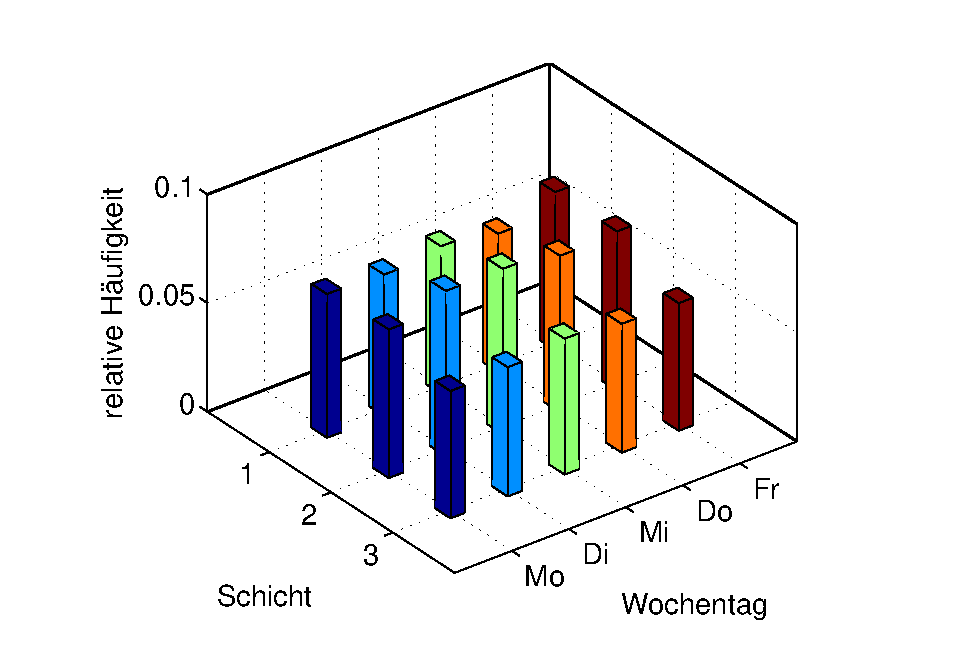
\includegraphics[width=0.5\textwidth]{Kapitel2/Bilder/image1}}
  \caption{System mit Ein- und Ausgangssignalen}
  \label{fig:EinAusSig}
\end{figure}

\noindent Einige Systeme lassen sich direkt mit algebraischen Gleichungen beschreiben. Ein Beispiel für ein solches System ist ein Spannungsteiler, bei dem sich die Ausgangsspannung direkt aus der Eingangsspannung
und dem Widerstandsverhältnis ergibt. Systeme, die sich über algebraische Gleichungen beschreiben lassen, besitzen keine Energiespeicher. Oftmals finden bei praktischen Anwendungen aber Einschwingvorgänge statt. Ursache für diese Einschwingvorgänge sind Energiespeicher, deren
Zustände sich durch eine Anregung ändern. Ein Beispiel für ein System mit Energiespeicher ist ein
RC-Tiefpass, bei dem ein Kondensator über einen Widerstand aufgeladen wird. Die Ausgangsspannung
des Kondensators ist eine Funktion der Zeit. Systeme mit Energiespeichern werden als dynamische Systeme bezeichnet. Dynamische Systeme beschreiben viele aus dem Alltag bekannte Prozesse. Beispiele sind Pendelbewegungen, das Verhalten elektrischer Schaltungen mit Kondensatoren und Spulen sowie thermische und chemische Prozesse. Es wird sich zeigen, dass die Systembeschreibung dynamischer Systeme aus einer oder mehreren Differentialgleichungen besteht.\newline
Auf Basis der mathematischen Beschreibung werden in diesem Kapitel wesentliche Systemeigenschaften
eingeführt. Diese Diskussion führt zur Untergruppe linearer, zeitinvarianter Systeme. Viele Vorgänge oder Prozesse lassen sich zumindest näherungsweise als lineare, zeitinvariante Systeme beschreiben. Die Eigenschaften Linearität und Zeitinvarianz erlauben eine vergleichsweise übersichtliche Beschreibung und vergleichsweise einfache Berechnung der Systemantwort. Dazu werden unterschiedliche
Verfahren vorgestellt.\newline
An einem Projekt mit Feder-Masse-Systemen werden lineare und nichtlineare Systeme theoretisch und experimentell miteinander verglichen.

\subsection{Beschreibung zeitkontinuierlicher Systeme mit Differentialgleichungen}\label{threeone}

Viele Systeme lassen sich über lineare Differentialgleichungen mit konstanten Koeffizienten beschreiben. In diesem Abschnitt werden einige einführende Beispiele vorgestellt.

\subsubsection{Beispiel RC-Netzwerk}
Die Beschreibung elektrischer Systeme erfolgt unter anderem über mathematische Gleichungen für die
beteiligten passiven Bauelemente. Tabelle \ref{tab:threeone} stellt die Bauelemente-Gleichungen für Widerstand, Kapazität und Induktivität zusammen [Alba04, ühr06].


\begin{table}[H]
\setlength{\arrayrulewidth}{.1em}
\caption{Thermische Bauelemente und ihre mathematische Beschreibung}
\setlength{\fboxsep}{0pt}%
\colorbox{lightgray}{%
\arrayrulecolor{white}%
\begin{tabular}{| wc{4cm} | wc{6cm} | wc{6cm} |}
\hline\xrowht{12pt}
{\fontfamily{phv}\selectfont
\textbf{Bauelement}} & 
\multicolumn{2}{c|}{\fontfamily{phv}\selectfont
\textbf{\textbf{Bauelemente-Gleichungen}}}\\ \hline \xrowht{25pt}

\fontfamily{phv}\selectfont{Widerstand} &
$U_{R}(t) = R\cdot i_{R}(t)$ &
$i_{R}(t) = \frac{1}{R}\cdot U_{R}(t)$\\ \hline  \xrowht{40pt}

\fontfamily{phv}\selectfont{Kapazität} &
$ U_{C}(t) = \frac{1}{C}\cdot \int\limits _{-\infty }^{t} i_{C}(\tau) \; d\tau$ &
$i_{C}(t) = C\cdot  \frac{dU_{C}}{dt}$\\ \hline\xrowht{40pt}

\fontfamily{phv}\selectfont{Induktivität} &
$ U_{L}(t) = L\cdot \frac{di_{L}}{dt}$ &
$i_{L}(t) = \frac{1}{L} \cdot \int\limits _{-\infty }^{t} U_{L}(\tau) \; d\tau$\\ \hline 

\end{tabular}%
}
\label{tab:threeone}
\end{table}

\bigskip

\noindent Darüber hinaus werden ideale Strom- und/oder Spannungsquellen angesetzt, die unabhängig von ihrer Belastung immer definierte Ausgangssignale liefern. Abweichungen von diesen als ideal angenommenen Quellen werden über diskrete Bauelemente wie Innenwiderstände beziehungsweise Innenleitwerte modelliert.\newline
Die Beschreibung eines Verbundes von Bauelementen erfolgt über Bilanzen und Nebenbedingungen.
Für elektrische Schaltungen ist die Bilanzgleichung bekannt als Knotengleichung.

\begin{equation}\label{eq:threeone}
\sum_{m-1}^{M}i_{m}(t)=0
\end{equation}

\noindent Die Maschengleichung stellt die entsprechende Nebenbedingung dar.

\begin{equation}\label{eq:threetwo}
\sum_{n-1}^{N}U_{n}(t)=0
\end{equation}

\noindent Bild \ref{fig:RCSchaltbild} zeigt ein einfaches Netzwerk bestehend aus einer Spannungsquelle $U_{E}(t)$, einem Widerstand R und einem Kondensator mit der Kapazität C.
\begin{figure}[ht]
  \centerline{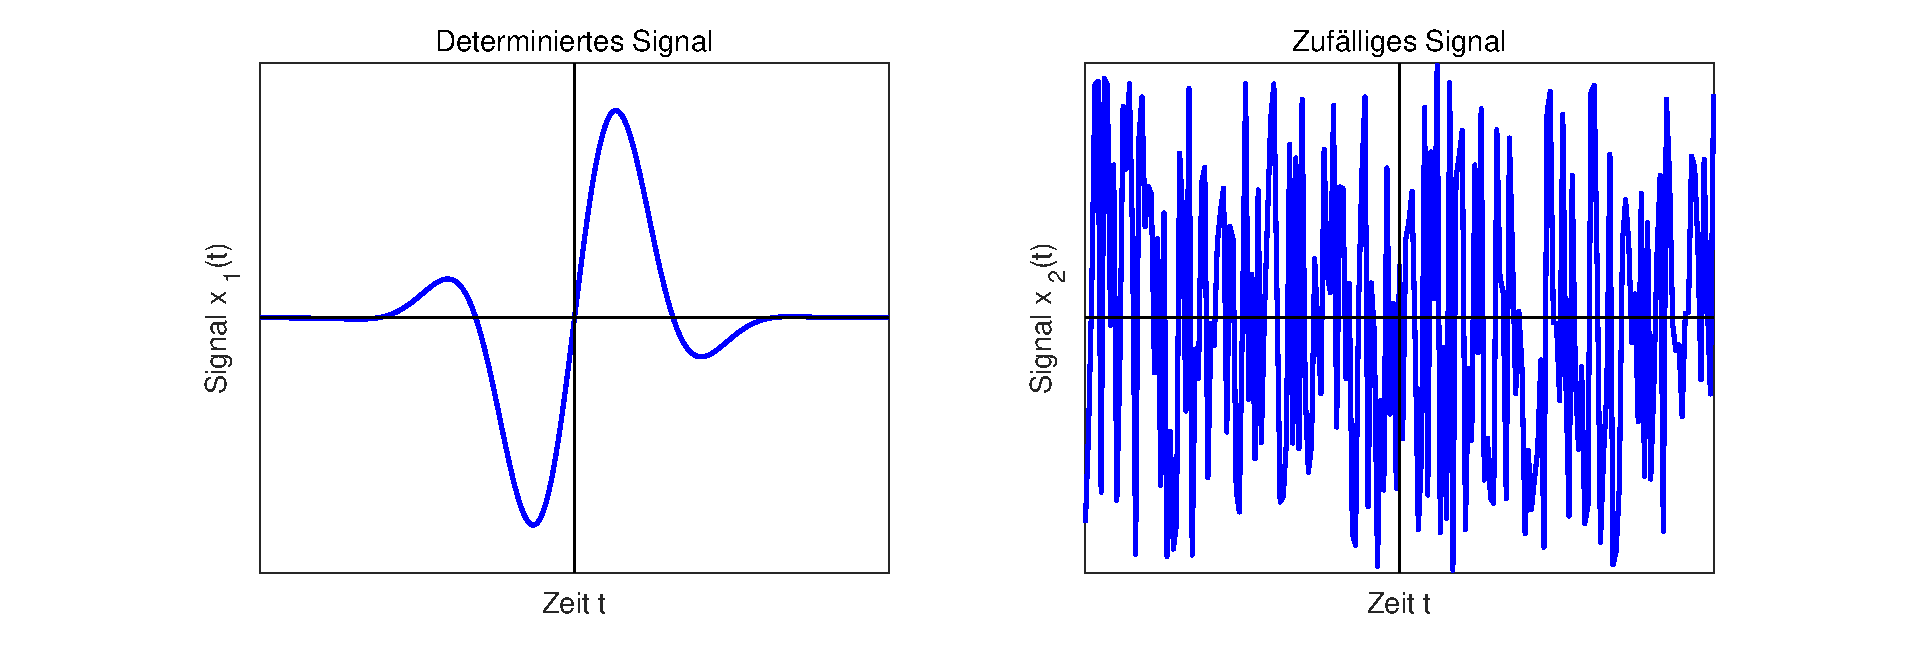
\includegraphics[width=0.32\textwidth]{Kapitel2/Bilder/image2}}
  \caption{Schaltbild für das Beispiel RC-Netzwerk}
  \label{fig:RCSchaltbild}
\end{figure}

\noindent Für das Einschalten einer Konstant-Spannungsquelle $U_{E}(t)$  soll die Spannung $U_{A}(t)$ am Kondensator berechnet werden. Die Spannung $U_{A}(t)$  wird zum Einschaltzeitpunkt $t=0$ zu $U_{A}(t)=0$ angenommen.
Dieser Zustand wird als Anfangszustand bezeichnet.

\noindent Bei der Anordnung lädt ein Strom i(t) die Kapazität C auf. Der Strom wird solange fließen, bis die Spannungsdifferenz an dem Widerstand R zu null wird. Sind die Spannungsdifferenzen ausgeglichen, befindet sich das System im Gleichgewicht. Zur mathematischen Beschreibung wird die Knotengleichung

\begin{equation}\label{eq:threethree}
i_{R}(t) = i_{C}(t) = i(t)
\end{equation}

\noindent Und die Maschengleichung

\begin{equation}\label{eq:threefour}
U_{E}(t) - U_{R}(t) - U_{A}(t)= U_{E}(t) - i_{R}(t)\cdot R - U_{A}(t) = 0
\end{equation}

\noindent aufgestellt. Wird der Strom $i_{R}(t)$ durch den Strom $i_{C}(t)$ ausgedrückt, ergibt sich

\begin{equation}\label{eq:threefive}
i_{R}(t) = i_{C}(t) = C\cdot \frac{d U_{A}}{dt}
\end{equation}

\noindent Einsetzen in die Maschengleichung führt nach Umstellen zu der linearen Differentialgleichung

\begin{equation}\label{eq:threesix}
U_{E}(t) = R\cdot C \frac{d U_{A}}{dt} + U_{A}(t)
\end{equation}

\noindent Bei der Differentialgleichung handelt es sich um eine lineare Differentialgleichung erster Ordnung mit konstanten Koeffizienten. Die Lösung dieser Differentialgleichung kann über eine sogenannte Vier-Schritt-Methode berechnet werden, auf die in Abschnitt \ref{threethree} ausführlich eingegangen wird. Bei Anregung des Systems mit einem Spannungssprung der Höhe $U_{0}$ am Eingang ergibt sich das Ausgangssignal zu

\begin{equation}\label{eq:threeseven}
U_{A}(t) = U_{0}\cdot (1-e^{\frac{t}{R\cdot C}})\cdot \sigma (t)
\end{equation}

\noindent Bild \ref{fig:RCEinschwingung} zeigt das Einschwingverhalten der Ausgangsspannung $U_{A}(t)$ für eine zum Zeitpunkt $t=0$ eingeschaltete Spannung $U_{0}= 5$ V, einen Widerstand von $R=5k\Omega$ und eine Kapazität von $C=4nF$.

\begin{figure}[ht]
  \centerline{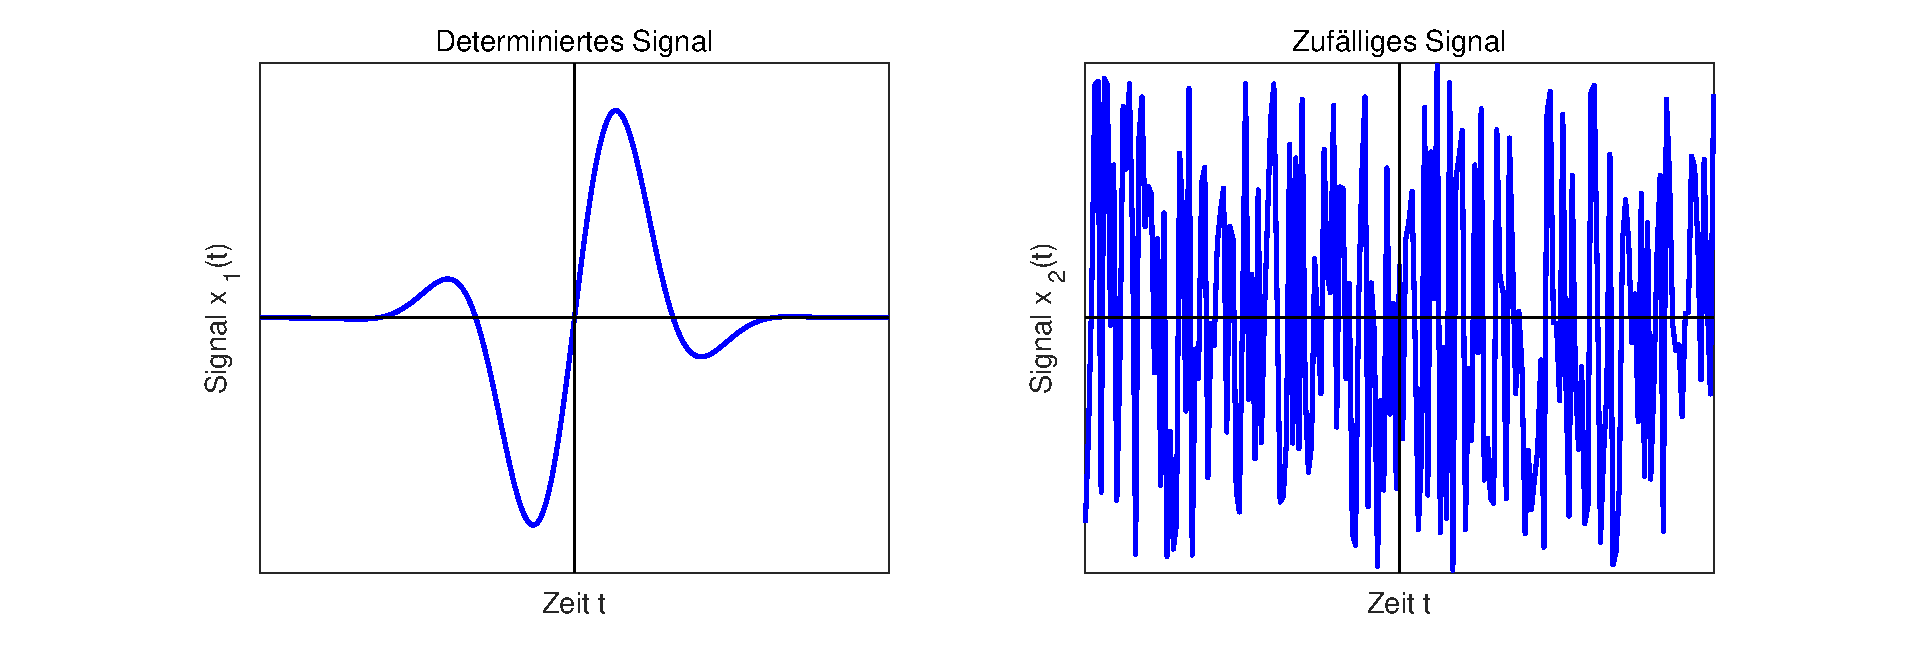
\includegraphics[width=0.5\textwidth]{Kapitel2/Bilder/image2}}
  \caption{Einschwingverhalten der Ausgangsspannung $U_{A}(t)$ eines RC-Netzwerks bei Anregung mit einem Spannungssprung von 0 auf 5 V}
  \label{fig:RCEinschwingung}
\end{figure}



\subsubsection{Beispiel Aufheizvorgang Wasserbad}
Ein Behälter, der ein Volumen V und eine Oberfläche A besitzt, ist mit Wasser gefüllt. Vereinfachend
wird angenommen, dass der Wärmeaustausch mit der Umgebung nur als Wärmeleitung über die Oberfläche
A stattfindet. Bild \ref{fig:RCEinschwingungBeispiel} beschreibt den Versuchsaufbau.

\begin{figure}[H]
  \centerline{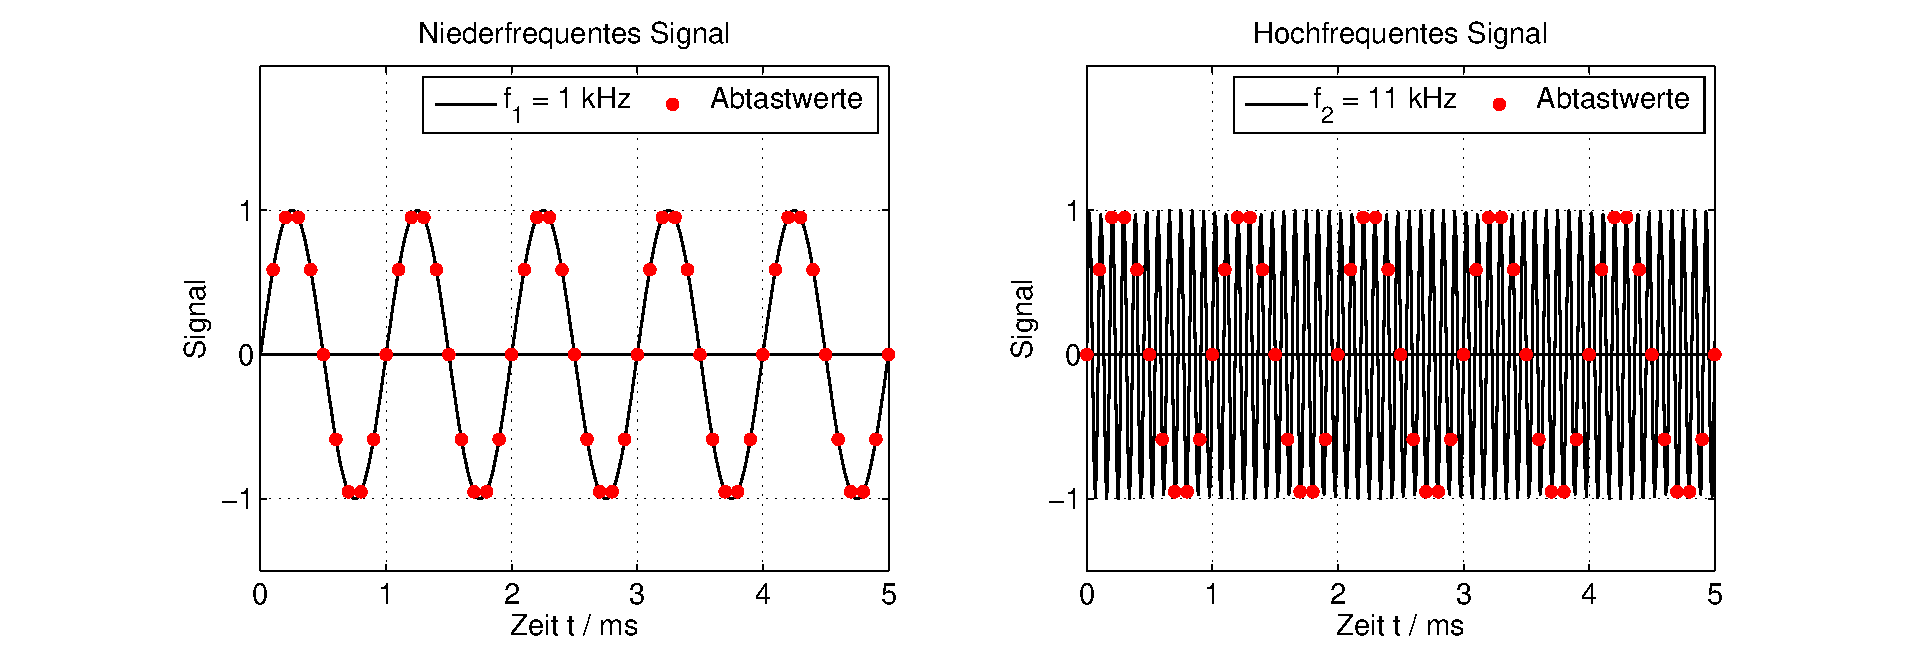
\includegraphics[width=0.5\textwidth]{Kapitel2/Bilder/image4}}
  \caption{Aufbau für das Beispiel Tauchsieder}
  \label{fig:RCEinschwingungBeispiel}
\end{figure}

\noindent Bis zu dem Zeitpunkt t = 0 entspricht die Wassertemperatur $\vartheta _{0}$ der Umgebungstemperatur $\vartheta _{U}$. Zum Zeitpunkt t = 0 wird ein Tauchsieder in das Wasser getaucht, der eine konstante elektrische Leistung $p _{EL}(t)$ umsetzt. Der Behälter tauscht wegen seiner steigenden Temperatur$\vartheta (t)$ > $\vartheta _{U}$über die Oberfläche A Wärme mit der Umgebung aus. Die Temperatur des Wassers wird sich solange erhöhen, bis sich ein Gleichgewicht zwischen der zugeführten Leistung $p _{EL}(t)$ und des über die Fläche A abgeführten Wärmestroms $p _{A}(t)$ einstellt.
Zur Modellierung werden die Bauelemente-Gleichungen für das System aufgestellt. Bei einer Temperaturdifferenz
$\Delta \vartheta $ an einer Fläche A mit der Wärmeübergangszahl $\alpha $ strömt durch die Oberfläche A der Wärmestrom $p_{A}$

\begin{equation}\label{eq:eight}
\Delta \vartheta(t) = \vartheta (t) - \vartheta _{U} = \frac{1}{\alpha \cdot A} \cdot p_{A}(t)
\end{equation}

\noindent Diese Beschreibung ist vergleichbar zum Ohmschen Gesetz. Der elektrischen Spannung $u(t)$ entspricht bei Wärmebilanzen die Temperaturdifferenz $\Delta \vartheta (t) $, dem elektrischen Strom $i(t)$ entspricht der Wärmestrom $p _{A}(t)$. Daraus resultiert die Definition des thermischen Widerstandes $R_{TH}$ zu

\begin{equation}\label{eq:threenine}
R_{TH} = \frac{\Delta \vartheta (t)}{p _{A}(t)}=\frac{1}{\alpha \cdot A}
\end{equation}

\noindent Auch die Wärmekapazität $C_{TH}$ ist in Anlehnung an die elektrische Kapazität definiert als der Quotient aus zugeführter Leistung $dp_{C}$ und der damit verbundenen Temperaturänderung $d \vartheta$

\begin{equation}\label{eq:threeten}
C_{TH}= \frac{dp_{C}}{d_{\vartheta}}
\end{equation}

\noindent Wird Gleichung \eqref{eq:threeten} nach $d \vartheta$ aufgelöst und eine Integration über die Zeit vorgenommen, so ergibt sich für die Temperaturänderung $ \Delta \vartheta$ des Wassers

\begin{equation}\label{eq:threeelf}
\Delta \vartheta (t) = \frac{1}{d_{C_{TH}}} \cdot \int\limits _{-\infty }^{t} p_{C} (\tau) \; d\tau
\end{equation}

\noindent Tabelle \ref{tab:threetwo} fasst die thermischen Bauelemente und ihre Bauelemente-Gleichungen zusammen.

\begin{table}[H]
\setlength{\arrayrulewidth}{.1em}
\caption{Thermische Bauelemente und ihre mathematische Beschreibung}
\setlength{\fboxsep}{0pt}%
\colorbox{lightgray}{%
\arrayrulecolor{white}%
\begin{tabular}{| wc{4cm} | wc{6cm} | wc{6cm} |}
\hline\xrowht{12pt}
{\fontfamily{phv}\selectfont
\textbf{Bauelement}} & 
\multicolumn{2}{c|}{\fontfamily{phv}\selectfont
\textbf{\textbf{Bauelemente-Gleichungen}}}\\ \hline \xrowht{25pt}

\fontfamily{phv}\selectfont{Wärmewiderstand} &
$\Delta \vartheta (t)=R_{TH} \cdot p _{A}(t) = \frac{1}{\alpha \cdot A} \cdot p _{A}(t)$ &
$p _{A}(t)=\alpha \cdot A \cdot \Delta \vartheta (t)$\\ \hline \xrowht{25pt}

\fontfamily{phv}\selectfont{Wärmekapazität} &
$ U_{R}(t) = R\cdot i_{R} (t)$ &
$U_{R}(t) = R\cdot i_{R}(t) $\\ \hline 

\end{tabular}%
}
\label{tab:threetwo}
\end{table}

\noindent Für die Bilanzen gelten sinngemäß die gleichen Beziehungen wie bei den elektrischen Größen. Die Maschenregel der Temperaturdifferenzen lautet

\begin{equation}\label{eq:threetwelve}
\sum_{n-1}^{N}\Delta \vartheta _{n} (t)=0
\end{equation}

\noindent und der Knotengleichung entspricht die Leistungsbilanz

\begin{equation}\label{eq:threethirteen}
\sum_{m-1}^{M} p_{m}(t)=0
\end{equation}

\noindent Zur Verknüpfung der elektrischen und thermischen Größen wird eine Leistungsbilanz erstellt. Die elektrische Leistung $p_{EL}(t)$ wird dem System von außen zugeführt. Über die Oberfläche gibt das System eine thermische Leistung $p_{A}(t)$ ab, sobald die Wassertemperatur über die Umgebungstemperatur steigt. Die Differenz beider Leistungen $p_{C}(t)$ wird dazu verwendet, die Wassertemperatur zu erhöhen.

\begin{equation}\label{eq:threefourteen}
p_{C}(t)=p_{EL}(t)-p_{A}(t)
\end{equation}

\noindent Einsetzen der Bauelement-Gleichungen ergibt die Differentialgleichung

\begin{equation}\label{eq:threefiveteen}
C_{TH} \cdot \frac{d \Delta \vartheta}{dt}=p_{EL}(t) - \alpha\cdot A\cdot \Delta\vartheta(t)
\end{equation}

\noindent beziehungsweise

\begin{equation}\label{eq:threesixteen}
\frac{C_{TH}}{\alpha\cdot A} \cdot \frac{\Delta\vartheta(t)}{dt} + \Delta\vartheta(t) = \frac{p_{EL}(t)}{\alpha\cdot A}
\end{equation}

\noindent Sie ist eine Differentialgleichung erster Ordnung mit konstanten Koeffizienten und entspricht in ihrer Struktur der Differentialgleichung des RC-Netzwerks. Die Lösung dieser Differentialgleichung ergibt sich nach der Vier-Schritt-Methode zu

\begin{equation}\label{eq:threeseventeen}
 \Delta\vartheta(t) = \vartheta_{0}\cdot (1-e^{\frac{-t}{T}})
\end{equation}

\noindent mit der Zeitkonstanten

\begin{equation}\label{eq:threeeightteen}
T=\frac{C_{TH}}{\alpha\cdot A}
\end{equation}

\noindent und der Temperatur $\vartheta_{0}$ von

\begin{equation}\label{eq:threenineteen}
\vartheta_{0} = \frac{p_{EL}(t)}{\alpha\cdot A}
\end{equation}

\noindent Bild \ref{fig:TempEinschwingung} stellt das Einschwingverhalten für eine Zeitkonstante T = 5 s und einen Temperatursprung $\vartheta_{0}$ von 20 K dar. Es entspricht grundsätzlich dem Einschwingverhalten des RC-Netzwerks.

\begin{figure}[H]
  \centerline{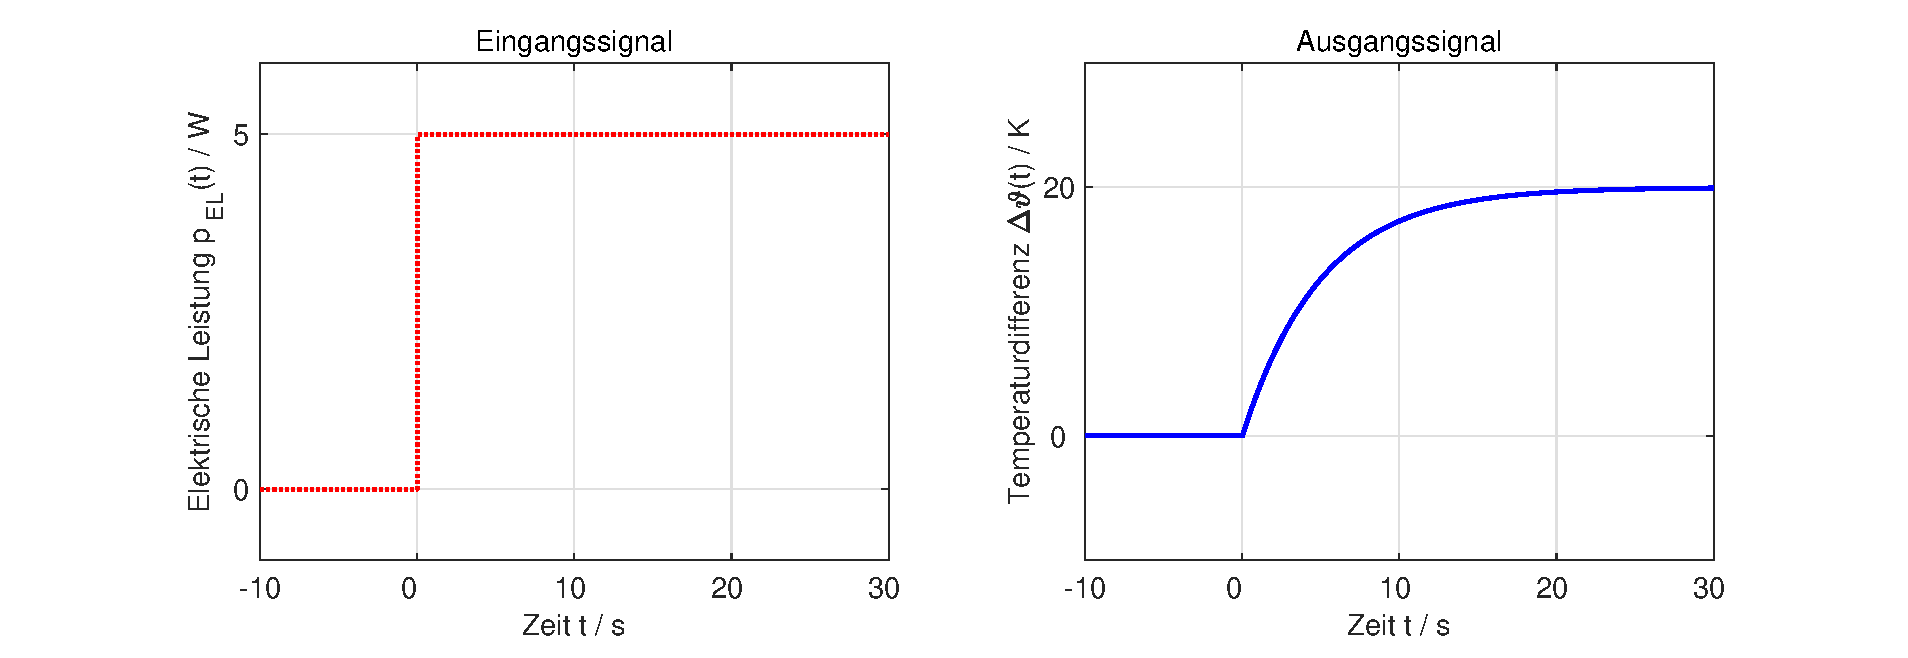
\includegraphics[width=1\textwidth]{Kapitel2/Bilder/image5}}
  \caption{Einschwingverhalten der Temperaturdifferenz bei einer sprungförmigen Anregung\\ mit einer konstanten elektrischen Leistung
}
  \label{fig:TempEinschwingung}
\end{figure}

\subsubsection{Beispiel Feder-Masse-Dämpfer-System}
Als weiteres Beispiel wird ein Feder-Masse-Dämpfer-System betrachtet, auf das eine äußere Kraft $F_{E}$ ausgeübt wird. Bild \ref{fig:FDSBeispiel} zeigt schematisch die Anordnung. Die Kraft $F_{E}$ greift an einem Körper der Masse m an und bewegt den Körper. Der Bewegung stehen die Trägheits-, Dämpfungs- und Rückstellkraft der Feder entgegen. Für die Anordnung soll die Auslenkung x berechnet werden, die sich bei
einer sprungförmig aufgebrachten Kraft FE an der Feder ergibt.

\begin{figure}[ht]
  \centerline{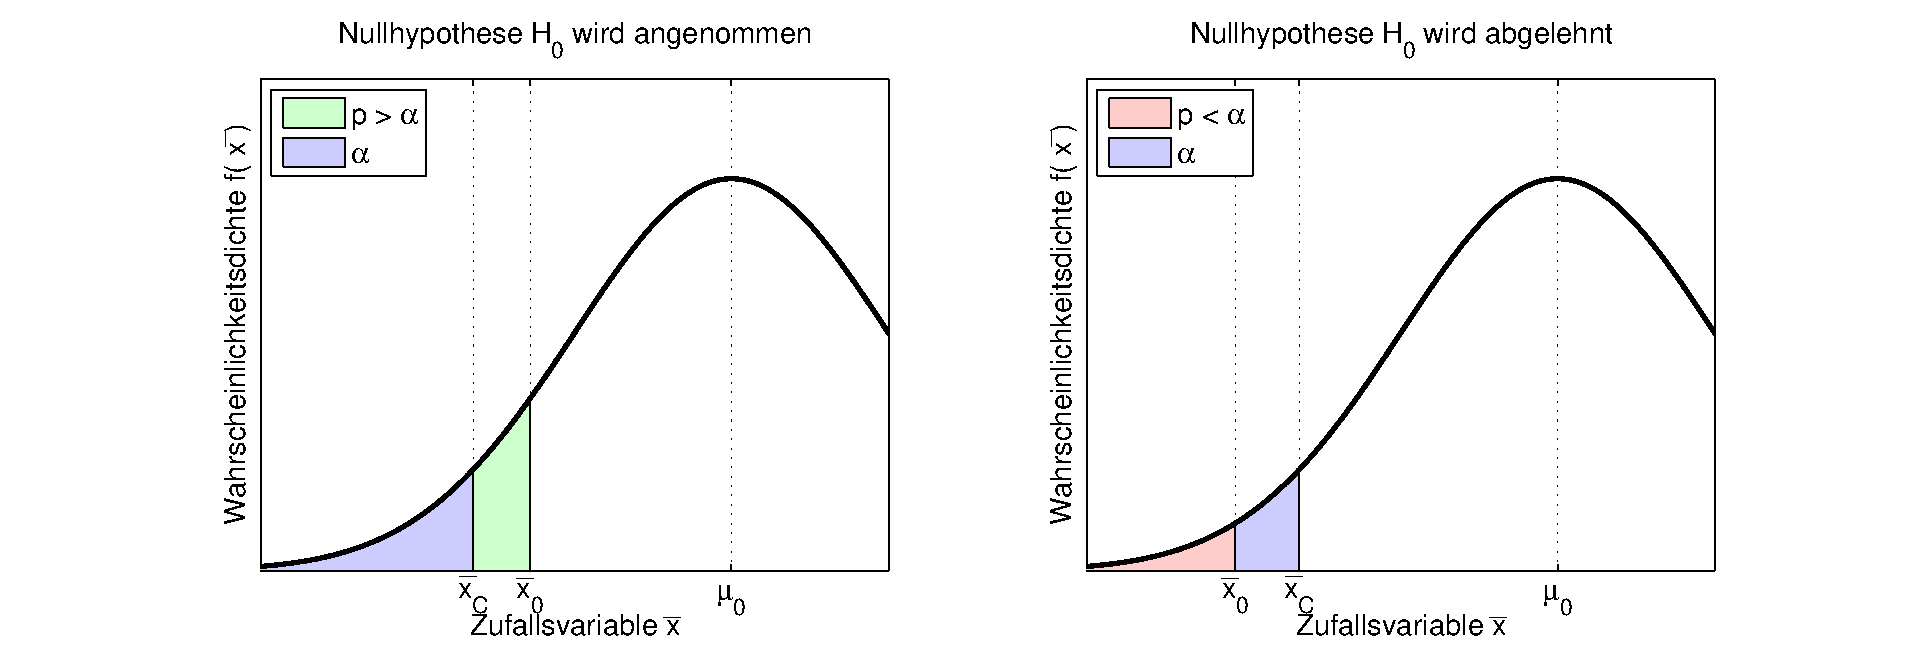
\includegraphics[width=0.5\textwidth]{Kapitel2/Bilder/image6}}
  \caption{Beispiel Feder-Dämpfer-System}
  \label{fig:FDSBeispiel}
\end{figure}

\noindent Genau wie bei dem elektrischen System lassen sich die mechanischen Bauelemente isoliert beschreiben. Tabelle \ref{tab:threethree} fasst mechanisch translatorische Bauelemente und ihre mathematische Beschreibung
zusammen.

\begin{table}[H]
\setlength{\arrayrulewidth}{.1em}
\caption{Thermische Bauelemente und ihre mathematische Beschreibung}
\setlength{\fboxsep}{0pt}%
\colorbox{lightgray}{%
\arrayrulecolor{white}%
\begin{tabular}{| wc{5.5cm} | wc{5.2cm} | wc{5.2cm} |}
\hline\xrowht{15pt}
{\fontfamily{phv}\selectfont
\textbf{Bauelement}} & 
\multicolumn{2}{c|}{\fontfamily{phv}\selectfont
\textbf{\textbf{Bauelemente-Gleichungen}}}\\ \hline \xrowht{40pt}

\fontfamily{phv}\selectfont{Feder mit Federkonstante c} &
$F_{C} \left(t\right)=c\cdot \int\limits _{-\infty }^{t}v\left(\tau \right){\rm \; }d\tau  =c\cdot x\left(t\right)$ & $v\left(t\right)=\frac{1}{c} \cdot \frac{dF_{C} }{dt} $ \\ \hline \xrowht{40pt}

\fontfamily{phv}\selectfont{Masse m} &
$F_{M} \left(t\right)=m\cdot a\left(t\right)=m\cdot \frac{dv}{dt} $ & $v\left(t\right)=\frac{1}{m} \cdot \int\limits _{-\infty }^{t}F_{M} \left(\tau \right){\rm \; }d\tau  $ \\ \hline\xrowht{40pt}

\fontfamily{phv}\selectfont{Viskose Reibung / Dämpfer D} &
$F_{D} \left(t\right)=D\cdot v\left(t\right)=D\cdot \frac{dx}{dt} $ & $v\left(t\right)=\frac{1}{D} \cdot F_{D} \left(t\right)$\\ \hline\xrowht{40pt}

\fontfamily{phv}\selectfont{Gleitreibung} & 
$F_{G} \left(t\right)=\mu \cdot F_{N} \left(t\right)\cdot sgn\left(v\left(t\right)\right)$ & \fontfamily{phv}\selectfont{keine Invertierung möglich} \\ \hline 
\end{tabular}%
}
\label{tab:threethree}
\end{table}


\noindent Auch in der Mechanik werden Gleichungen angesetzt, die den Maschen- und Knotenregeln entsprechen. Der Maschenregel entspricht die Kräftesumme

\begin{equation}\label{eq:threetwenty}
\sum_{n-1}^{N} F_{n}(t)=0
\end{equation}

\noindent Durch mechanische Kopplung lässt sich eine Aussage über die Auslenkung der verschiedenen Bauelemente des Systems machen. In diesem Beispiel sind Masse, Feder und Dämpfer starr miteinander gekoppelt. Die Auslenkungen x(t) für Masse, Feder und Dämpfer sind damit identisch. Die Anwendung der Kräftebilanz ergibt unter Berücksichtigung der unterschiedlichen Kraftrichtungen

\begin{equation}\label{eq:threetwentyone}
F_{E}(t)-F_{M}(t)-F_{D}(t)-F_{C}(t)=
F_{E}(t)-m\cdot a(t)-D\cdot v(t)-c\cdot x(t)=0
\end{equation}

\noindent und der Zusammenhang zwischen der Auslenkung $x(t)$ und der angreifenden Kraft $F_{E}(t)$ kann als Differentialgleichung dargestellt werden.

\begin{equation}\label{eq:threetwentytwo}
F_{E}(t)=m\cdot \frac{d^2x}{dt^2}+D\cdot \frac{dx}{dt}+c\cdot x(t)
\end{equation}

\noindent Es handelt sich wieder um eine lineare Differentialgleichung mit konstanten Koeffizienten. Die Ordnung der Differentialgleichung entspricht der höchsten Ableitung, in diesem Beispiel ist die Ordnung N = 2. Die Lösung der Differentialgleichung kann für ein definiertes Eingangssignal und eine definierte Anfangsbedingung wie bei dem elektrischen System mit der Vier-Schritt-Methode erfolgen. Für ein System, das sich zum Zeitpunkt t = 0 in Ruhelage befindet und mit einem Kraftsprung am Eingang

\begin{equation}\label{eq:threetwentythree}
F_{E}(t)=F_{0}\cdot \sigma(t)
\end{equation}

\noindent angeregt wird, ergibt sich bei geringer Dämpfung D die Lösung


\begin{equation}\label{eq:threetwentyfour}
x(t) = \frac{F_{0}}{c} \cdot \left(1+\frac{e^{-\frac{D}{2\cdot m} \cdot t} }{\sqrt{1-\left(\frac{D}{2\cdot \sqrt{m\cdot c} } \right)^{2} } } \cdot \sin \left(\sqrt{\frac{c}{m} -\left(\frac{D}{2\cdot m} \right)^{2} } \cdot t-\varphi \right)\right)\cdot \sigma \left(t\right)
\end{equation}

\noindent Auf die Berechnung dieses  inschwingverhaltens wird später noch genauer eingegangen. Das Einschwingverhalten ist in Bild \ref{fig:AusblendeigenschaftImpulsfunktion} für eine Federkonstante von c = 100 N/m, eine Dämpfung von $D = 0.5 N\cdot s/m$, eine Masse m = 10 g und eine Kraft $F_{0}= 0.2 N$  dargestellt.

\begin{figure}[ht]
  \centerline{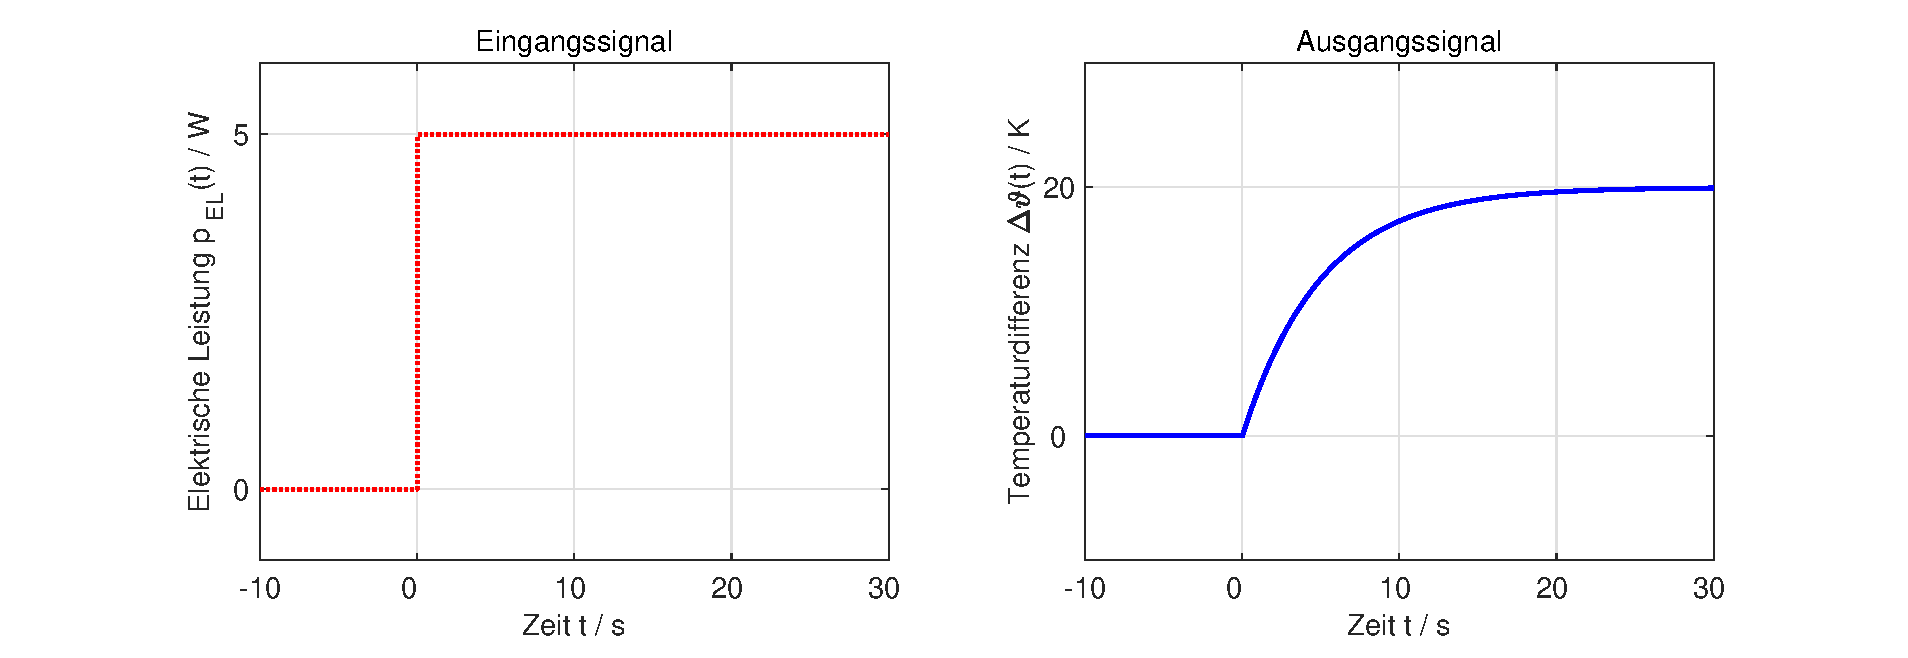
\includegraphics[width=1\textwidth]{Kapitel2/Bilder/image5}}
  \caption{Einschwingverhalten des Feder-Masse-Dämpfer-Systems bei einer sprungförmigen Anregung mit einer Kraft von $F_{0}= 0.2 N$}
  \label{fig:AusblendeigenschaftImpulsfunktion}
\end{figure}

\subsubsection{Resümee zu den Beispielen}
Viele Systeme lassen sich wie die hier diskutierten Systeme zumindest in guter Näherung durch lineare
Differentialgleichungen mit konstanten Koeffizienten beschreiben.

\begin{equation}\label{eq:threetwentyfive}
a_{0}\cdot y(t) + a_{1}\cdot \frac{dy}{dt}+a_{2}\cdot \frac{d^2y}{dt^2}+ ... +a_{n}\cdot \frac{d^Ny}{dt^N}=
b_{0}\cdot u(t) + b_{1}\cdot \frac{du}{dt}+b_{2}\cdot \frac{d^2u}{dt^2}+ ... +b_{m}\cdot \frac{d^Mu}{dt^M}
\end{equation}

\noindent Die Beschreibung des Systems mit Differentialgleichungen wird als Modellbildung bezeichnet. Sie ist für praktische Aufgabenstellungen anspruchsvoll und oft nur mit Erfahrung zu lösen. Auf die Modellbildung wird in Kapitel \textbf{Fehler! Verweisquelle konnte nicht gefunden werden}. ausführlich eingegangen, und es wird ein Leitfaden zur Modellierung von Systemen vorgestellt.


\subsection{Grundlegende Eigenschaften zeitkontinuierlicher Systeme} \label{threetwo}

Im Abschnitt \ref{threeone} werden unterschiedliche Systeme beschrieben. Die mathematische Modellierung führt bei diesen Beispielen zu linearen Differentialgleichungen mit konstanten Koeffizienten. In diesem Abschnitt werden grundlegende Eigenschaften von Systemen diskutiert. Es wird sich zeigen, dass lineare Differentialgleichungen mit konstanten Koeffizienten lineare, zeitinvariante Systeme beschreiben.

\subsubsection{Linearität}
Für den Linearitätsnachweis eines Systems müssen die Systemantworten $y_{1}(t)$ und $y_{2}(t)$ auf die linear unabhängigen Eingangssignale $u_{1}(t)$ und $u_{2}(t)$ bekannt sein. Ein System ist linear, wenn es auf eine Linearkombination von Eingangssignalen

\begin{equation}\label{eq:threetwentysix}
u_{t} = v_{1}\cdot u_{1}(t) +v_{2}\cdot u_{2}(t)
\end{equation}

\noindent mit derselben Linearkombination der entsprechenden Kombination von Ausgangssignalen reagiert.

\begin{equation}\label{eq:threetwentyseven}
y_{t} = v_{1}\cdot y_{1}(t) +v_{2}\cdot y_{2}(t)
\end{equation}

\noindent Der Nachweis der Linearität erfolgt über Einsetzen der Gleichungen in die Differentialgleichung.\bigskip

\noindent
\colorbox{lightgray}{%
\arrayrulecolor{white}%
\renewcommand\arraystretch{0.6}%
\begin{tabular}{ wl{16.5cm} }
{\fontfamily{phv}\selectfont{Beispiel: Linearität eines RC-Netzwerks} }
\end{tabular}%
}\bigskip

\noindent Ein RC-Netzwerk mit der Differentialgleichung

\begin{equation}\label{eq:threetwentyeight}
U_{E}(t) =R\cdot C\cdot \frac{dU_{A}(t)}{dt}+ U_{A}(t)
\end{equation}

\noindent soll auf Linearität untersucht werden. Die Systemantworten $U_{A1}(t)$ und $U_{A2}(t)$ ergeben sich mit der Differentialgleichung \ref{eq:threetwentyeight} zu

\begin{equation}\label{eq:threetwentynine}
U_{E1}(t) =R\cdot C\cdot \frac{dU_{A1}(t)}{dt}+ U_{A1}(t)
\end{equation}

\noindent beziehungsweise

\begin{equation}\label{eq:threethirty}
U_{E2}(t) =R\cdot C\cdot \frac{dU_{A2}(t)}{dt}+ U_{A2}(t)
\end{equation}

\noindent Wird das System mit der Linearkombination

\begin{equation}\label{eq:threethirtyone}
U_{E}(t) =\nu_{1}\cdot U_{E1}(t) +\nu_{2}\cdot U_{E2}(t)
\end{equation}

\noindent angeregt, ergibt sich

\begin{equation}\label{eq:threethirtytwo}
\begin{split} 
u_{E} \left(t\right) & = \nu _{1} \cdot u_{E1} \left(t\right)+\nu _{2} \cdot u_{E2} \left(t\right) \\ 
& = \nu _{1} \cdot \left(R\cdot C\cdot \frac{du_{A1} \left(t\right)}{dt} +u_{A1} \left(t\right)\right)+\nu _{2} \cdot \left(R\cdot C\cdot \frac{du_{A2} \left(t\right)}{dt} +u_{A2} \left(t\right)\right) \\ 
& = R\cdot C\cdot \left(\nu _{1} \cdot \frac{du_{A1} \left(t\right)}{dt} +\nu _{2} \cdot \frac{du_{A2} \left(t\right)}{dt} \right)+\left(\nu _{1} \cdot u_{A1} \left(t\right)+\nu _{2} \cdot u_{A2} \left(t\right)\right) \\ 
& = R\cdot C\cdot \frac{du_{A} \left(t\right)}{dt} +u_{A} \left(t\right) 
\end{split}
\end{equation}

\noindent Das Ausgangssignal $U_{A}(t)$ weist dieselbe Linearkombination auf wie das Eingangssignal.


\noindent
\colorbox{lightgray}{%
\arrayrulecolor{white}%
\renewcommand\arraystretch{0.6}%
\begin{tabular}{ wl{16.5cm} }
{\fontfamily{phv}\selectfont{Beispiel: Nichtlineares System}}
\end{tabular}%
}\bigskip

\noindent Der Strom $i_{D}(t)$  durch eine Diode als Funktion der anliegenden Spannung wird über die Shockley-Gleichung berechnet.

\begin{equation}\label{eq:threethirtythree}
i_{D}(t)=I_{S}\cdot (e^{\frac{U_{D}(t)}{n\cdot U_{T}}}-1)
\end{equation}

\noindent Die Diode soll auf Linearität untersucht werden. Die Systemantworten $i_{D1}(t)$  und $i_{D2}(t)$ ergeben sich mit der Shockley-Gleichung zu

\begin{equation}\label{eq:threethirtyfour}
i_{D1}(t)=I_{S}\cdot (e^{\frac{U_{D1}(t)}{n\cdot U_{T}}}-1)
\end{equation}

\noindent beziehungsweise

\begin{equation}\label{eq:threethirtyfive}
i_{D2}(t)=I_{S}\cdot (e^{\frac{U_{D2}(t)}{n\cdot U_{T}}}-1)
\end{equation}

\noindent Wird das System mit der Linearkombination

\begin{equation}\label{eq:threethirtysix}
U_{D}(t)=k_{1}\cdot U_{D1}(t) + k_{2}\cdot U_{D2}(t) 
\end{equation}

\noindent angeregt, ergibt sich der Diodenstrom

\begin{equation}\label{eq:threethirtyseven}
\begin{split}
i_{D}(t) & = I_{S} \cdot \left(e^{\frac{u_{D} \left(t\right)}{n\cdot U_{T} } } -1\right)=I_{S} \cdot \left(e^{\frac{\nu _{1} \cdot u_{D1} \left(t\right)+\nu _{2} \cdot u_{D2} \left(t\right)}{n\cdot U_{T} } } -1\right)=I_{S} \cdot \left(e^{\frac{\nu _{1} \cdot u_{D1} \left(t\right)}{n\cdot U_{T} } } \cdot e^{\frac{\nu _{2} \cdot u_{D2} \left(t\right)}{n\cdot U_{T} } } -1\right) \\ 
& \ne \nu _{1} \cdot I{}_{S} \cdot \left(e^{\frac{u_{D1} \left(t\right)}{n\cdot U_{T} } } -1\right)+\nu _{2} \cdot I{}_{S} \cdot \left(e^{\frac{u_{D2} \left(t\right)}{n\cdot U_{T} } } -1\right) = \nu _{1} \cdot i_{D1} \left(t\right)+\nu _{2} \cdot i_{D2} \left(t\right)
\end{split}
\end{equation}

\noindent Der Strom $i_{D}(t)$  durch die Diode ist nichtlinear zur Spannung $u_{D}(t)$, die an der Diode anliegt. Eine Diode ist damit ein nichtlineares Bauteil.\newline
Die Linearität von Systemen kann auch daran abgelesen werden, dass alle Signale und Ableitungen nur in linearen Summen auftreten. Ist ein System linear, kann ein Ausgangssignal dadurch berechnet werden, dass die Eingangssignale zerlegt, ihre jeweiligen Systemantworten berechnet und anschließend addiert werden. Dieses Prinzip wird als Superpositionsprinzip bezeichnet. Bild 3.8 zeigt Ein- und Ausgangssignale eines linearen Systems, das mit den Signalen $u_{1}(t)$, $u_{2}(t)$ und $u_{1}(t)$ + $u_{2}(t)$ angeregt wird. Das Ausgangssignal $y(t)$ setzt sich aus der Summe der Ausgangsignale $y_{1}(t)$ und $y_{2}(t)$ zusammen.

\begin{figure}[H]
  \centerline{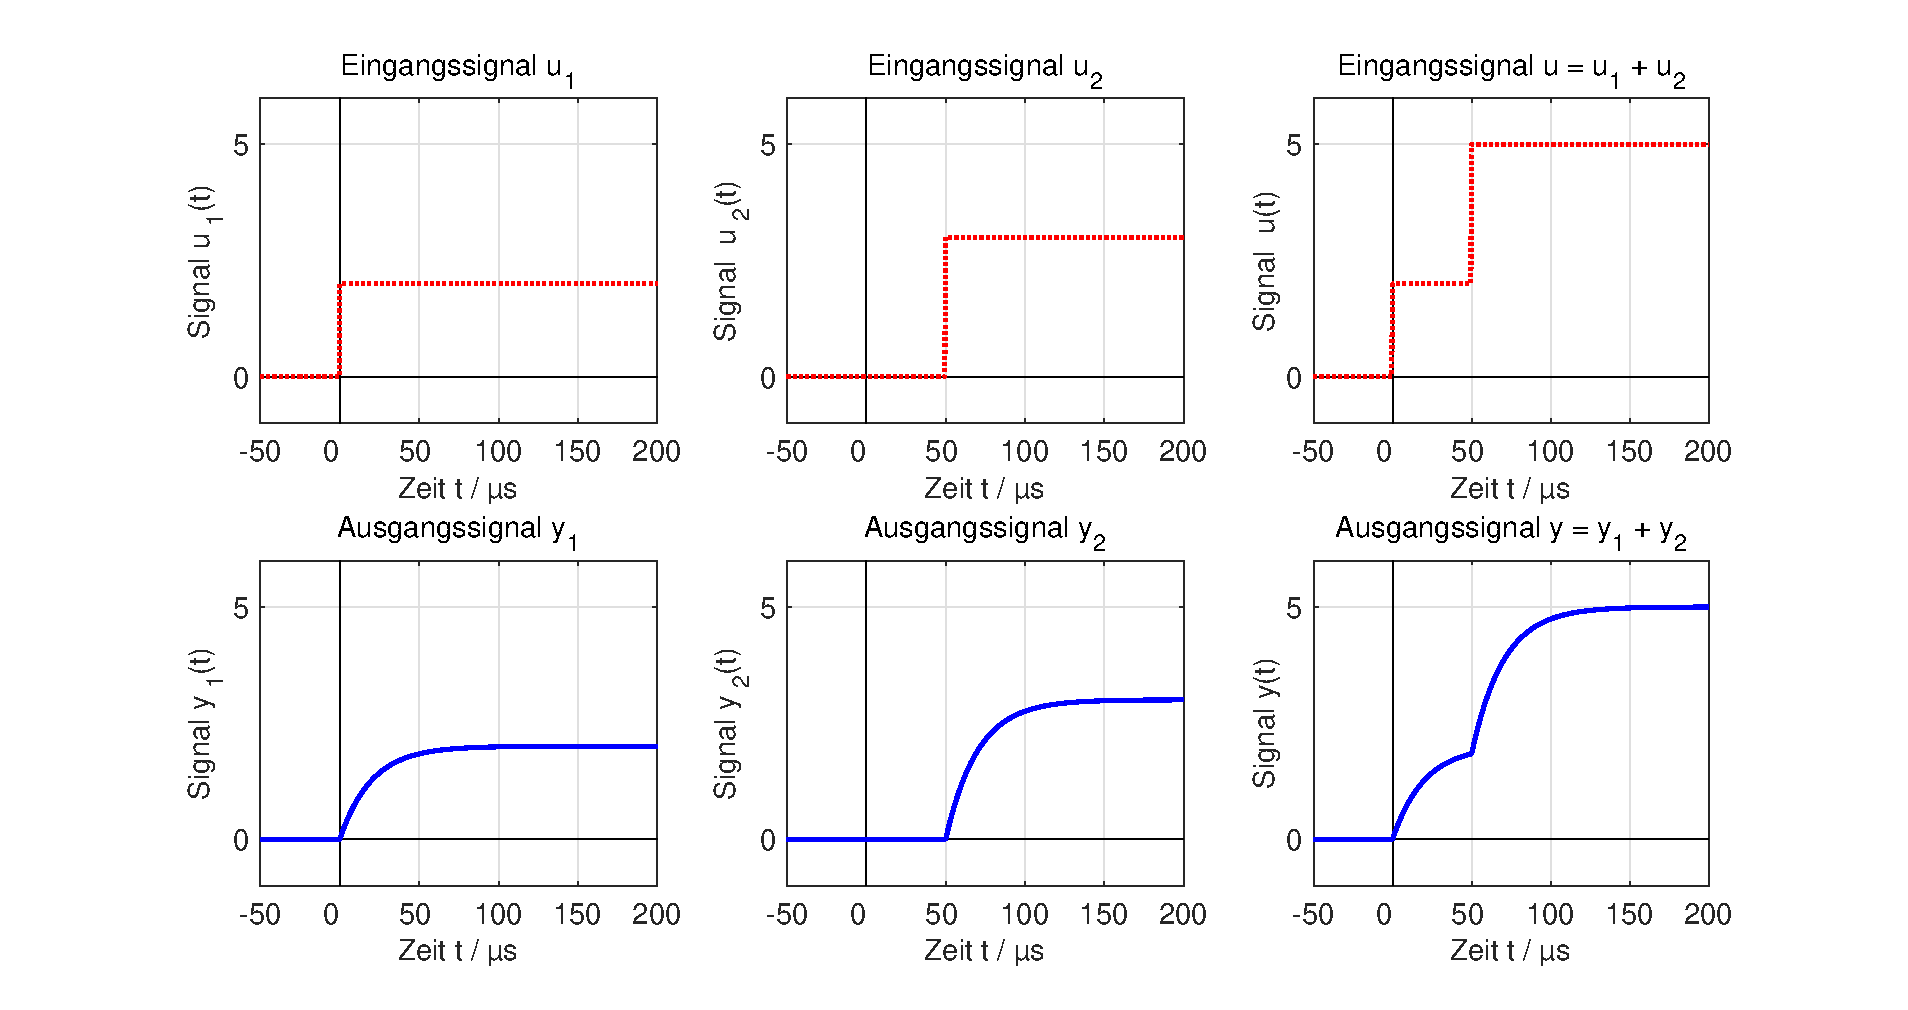
\includegraphics[width=1\textwidth]{Kapitel2/Bilder/image8}}
  \caption{Reaktion eines linearen Systems auf die Anregung mit einer Linearkombination von Signalen}
  \label{fig:Linearitat}
\end{figure}

\noindent Linearität ist eine idealisierte Eigenschaft eines Systems, zum Beispiel wird sich der Widerstand R nichtlinear verhalten, wenn in ihm eine hohe Verlustleistung umgesetzt wird, und er sich erhitzt. In der Praxis werden viele Prozesse oder Systeme linear beschrieben, obwohl diese idealisierte Annahme nur in definierten Grenzen gilt. Andererseits können auch nichtlineare Systeme näherungsweise linear beschrieben werden. Dazu wird in dem nichtlinearen System ein Arbeitspunkt definiert und kleine Abweichungen aus dem Arbeitspunkt werden als linear angenommen.\bigskip

\noindent
\colorbox{lightgray}{%
\arrayrulecolor{white}%
\renewcommand\arraystretch{0.6}%
\begin{tabular}{ wl{16.5cm} }
{\fontfamily{phv}\selectfont
{Beispiel: Linearisierung einer Diodenkennlinie im Arbeitspunkt}}
\end{tabular}%
}\bigskip

\noindent Das nichtlineare Verhalten des Diodenstroms $i_{D}(t)$  als Funktion der Diodenspannung $u_{D}(t)$ soll in einem Arbeitspunkt mit der Spannung $u_{0}$ und dem Strom $i_{0}$ linearisiert werden. Bild \ref{fig:Linearisierung} verdeutlicht die Linearisierung um einen Arbeitspunkt grafisch.\bigskip

\begin{figure}[H]
  \centerline{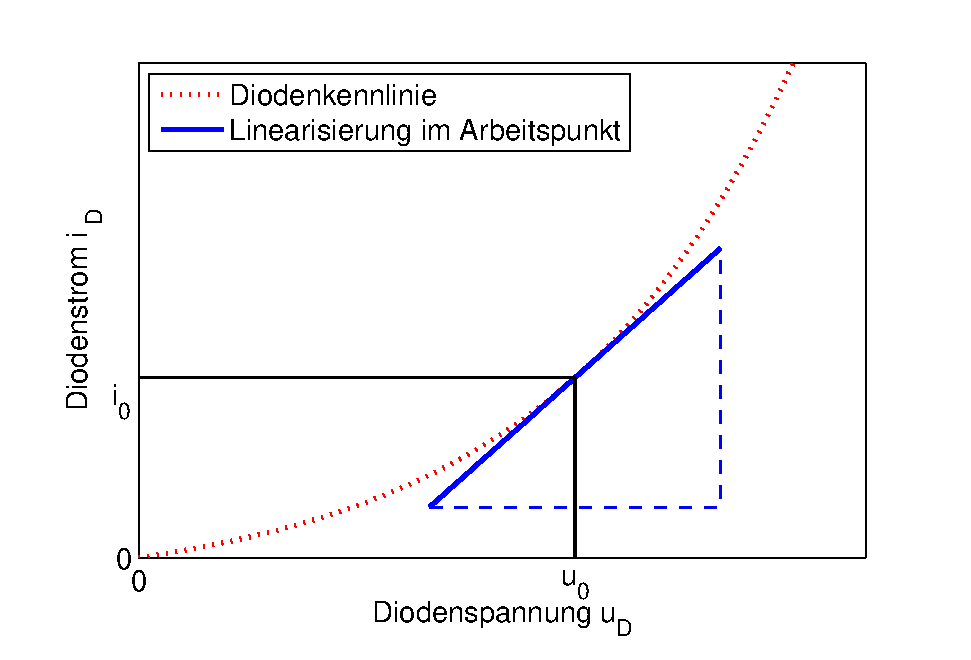
\includegraphics[width=0.5\textwidth]{Kapitel2/Bilder/image9}}
  \caption{Linearisierung um einen Arbeitspunkt am Beispiel der Diodenkennlinie}
  \label{fig:Linearisierung}
\end{figure}

\noindent In dem Arbeitspunkt $(u_{0}|i_{0})$ wird durch Ableitung der Shockley-Gleichung die Steigung der Tangente bestimmt.


\begin{equation}\label{eq:threethirtyeight}
m=\left. \frac{di_{D} }{du_{D} } \right|_{u_{D} =u_{0} } =\left. \frac{I_{S} }{n\cdot U_{T} } \cdot e^{\frac{u_{D} \left(t\right)}{n\cdot U_{T} } } \right|_{u_{D} =u_{0} } =\frac{I_{S} }{n\cdot U_{T} } \cdot e^{\frac{u_{0} }{n\cdot U_{T} } }
\end{equation}

\noindent Das Systemverhalten im Arbeitspunkt ergibt sich dann aus der Geradengleichung


\begin{equation}\label{eq:threethirtynine}
i_{D} \left(t\right)-i_{0} =\frac{I_{S} }{n\cdot U_{T} } \cdot e^{\frac{u_{0} }{n\cdot U_{T} } } \cdot \left(u_{D} \left(t\right)-u_{0} \right)=m\cdot \left(u_{D} \left(t\right)-u_{0} \right)
\end{equation}

\noindent Mit den Bezeichnungen

\begin{equation}\label{eq:threefourty}
\Delta i_{D}(t)=i_{D}(t)-i_{0}
\end{equation}

\begin{equation}\label{eq:threefourtyone}
\Delta U_{D}(t)=U_{D}(t)-U_{0}
\end{equation}

\noindent ergibt sich die lineare Beschreibungsform

\begin{equation}\label{eq:threefourtytwo}
\Delta i_{D}(t)=m\cdot \Delta U_{D}(t)
\end{equation}

\noindent Gleichung \ref{eq:threefourtytwo} stellt eine lineare Näherung für das nichtlineare System Diode im Arbeitspunkt $(u_{0}|i_{0})$ dar. Bild \ref{fig:Linearisierung} macht jedoch deutlich, dass diese Linearisierung nur für sehr kleine Werte $\Delta u_{D}$ ausreichend präzise ist.

\subsubsection{Zeitinvarianz}\label{threetwotwo}
Ein System reagiert auf ein Eingangssignal $u(t)$ mit einer Systemantwort $y(t)$. Ist das System zeitinvariant, so reagiert das System auf das zeitlich verschobene  Eingangssignal $u(t-t_{0})$ mit dem verschobenen Ausgangsignal $y(t-t_{0})$. Zeitinvariante Systeme reagieren also unabhängig vom Startzeitpunkt der Anregung auf gleiche Eingangssignale mit gleichen Ausgangssignalen.\bigskip

\noindent
\colorbox{lightgray}{%
\arrayrulecolor{white}%
\renewcommand\arraystretch{0.6}%
\begin{tabular}{ wl{16.5cm} }
{\fontfamily{phv}\selectfont{Beispiel: Zeitinvarianz eines Feder-Masse-Dämpfer Systems }}
\end{tabular}%
}\bigskip

\noindent Das Feder-Masse-Dämpfer System mit der Differentialgleichung

\begin{equation}\label{eq:threefourtythree}
F_{E}(t)= m\cdot \frac{d^2x}{dt^2}+D\cdot \frac{dx}{dt} + c\cdot x(t)
\end{equation}

\noindent soll auf Zeitinvarianz untersucht werden. Dazu werden alle Ausdrücke t durch den Ausdruck $t - t_{0}$ ersetzt. Unter der Annahme, dass die Koeffizienten m, D und c nicht ändern, ergibt sich die Differentialgleichung

\begin{equation}\label{eq:threefourtyfour}
F_{E}(t-t_{0})= m\cdot \frac{d^2x(t-t_{0})}{dt^2}+D\cdot \frac{dx(t-t_{0})}{dt} + c\cdot x(t-t_{0})
\end{equation}

\noindent Wird das Eingangssignal um $t_{0}$ verschoben, wird auch das Ausgangsignal um $t_{0}$ verschoben.
\clearpage
\begin{figure}[H]
  \centerline{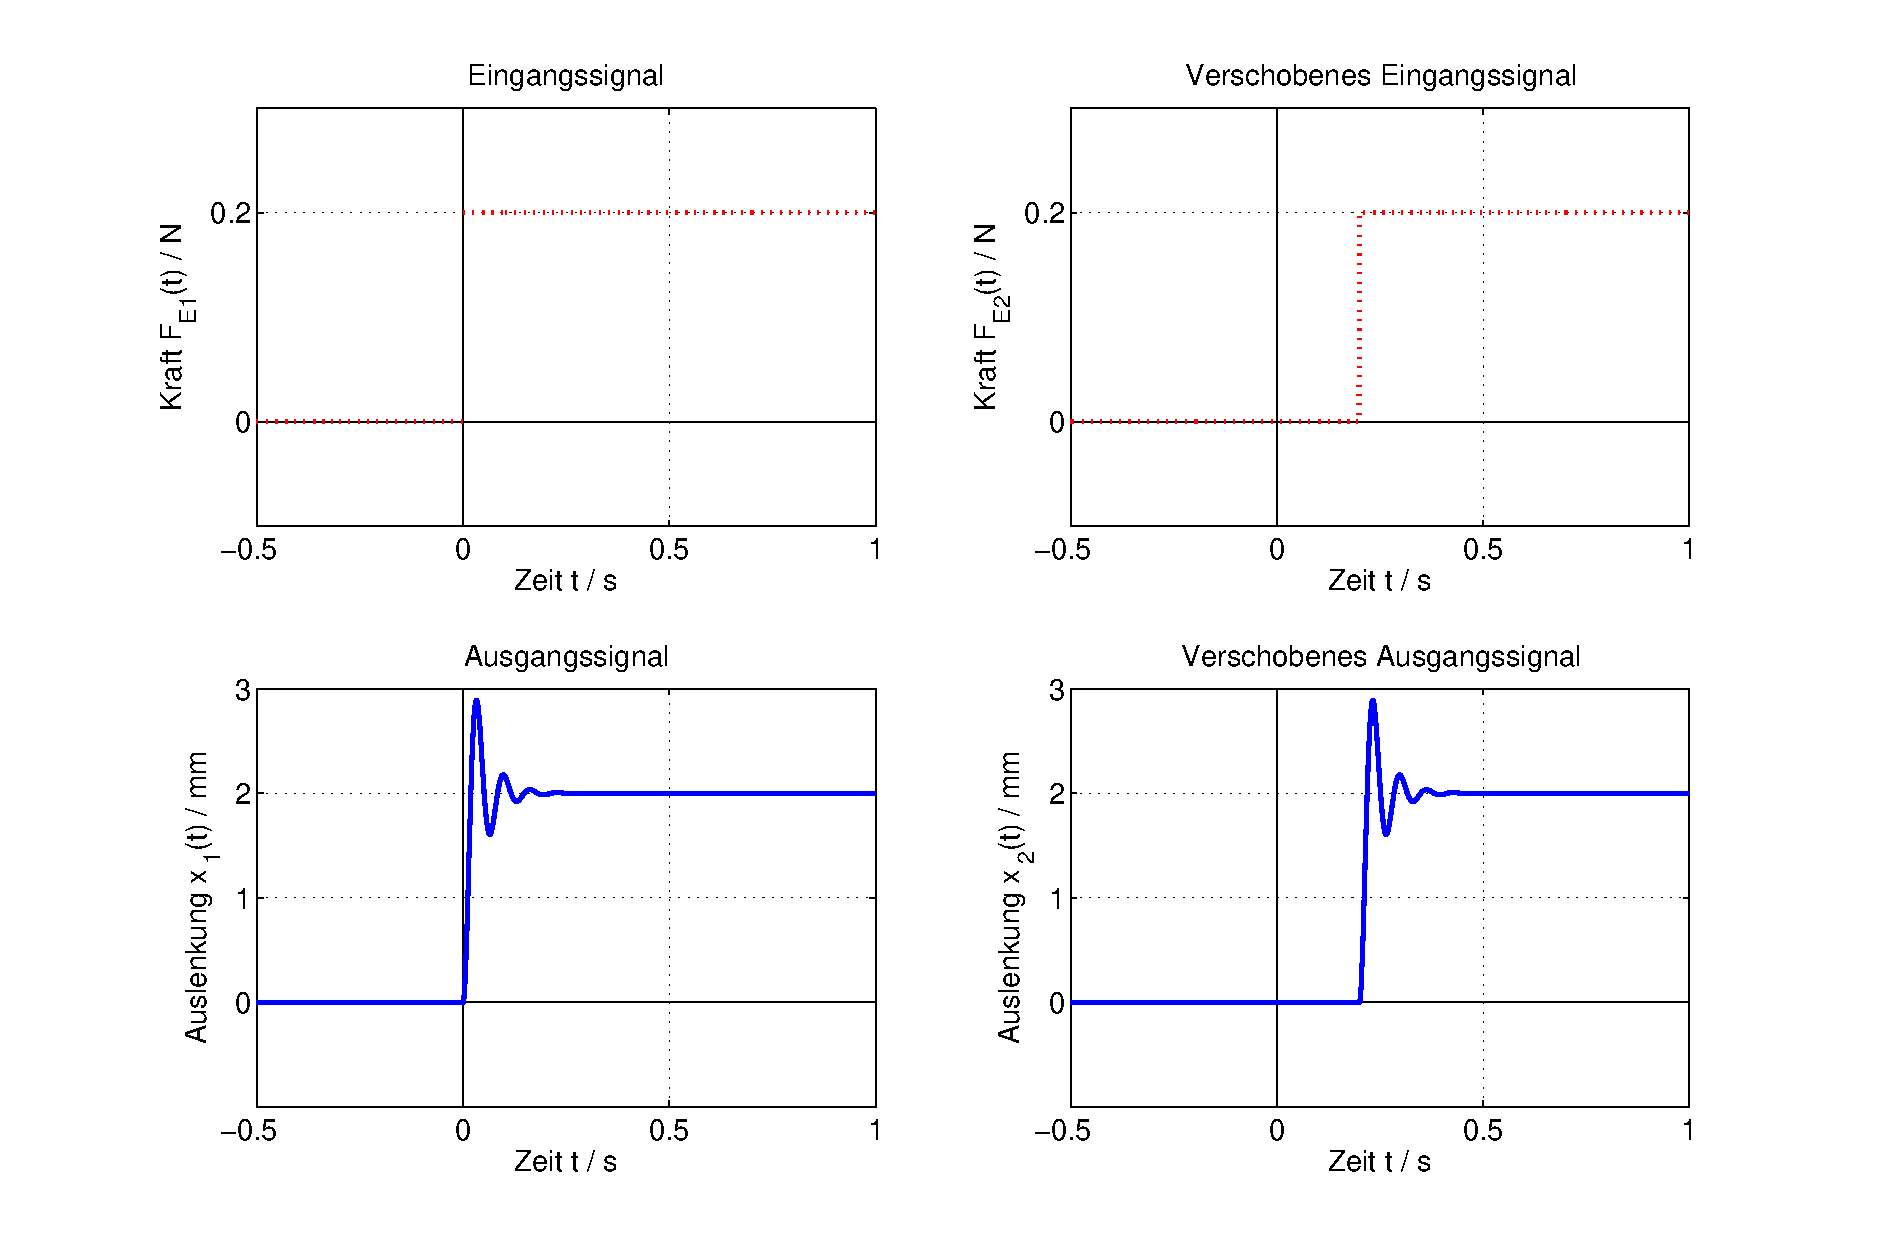
\includegraphics[width=1\textwidth]{Kapitel2/Bilder/image10}}
  \caption{Reaktion eines zeitinvarianten Systems auf die Anregung mit einem um $t_{0} = 0.2 s$\\ zeitverschobenen Signal} 
  \label{fig:Zeitinvarianz}
\end{figure}

\noindent Wird ein System mit einer linearen Differentialgleichung beschrieben, die konstante Koeffizienten
aufweist, ist das Systemverhalten von der Zeit unabhängig, und das System ist zeitinvariant. Ändern sich die Koeffizienten der Differentialgleichung als Funktion der Zeit t, verändert sich das System mit der Zeit. Es ist zeitvariant.\newline
Auch die Zeitinvarianz ist eine Eigenschaft, die oft nur näherungsweise erfüllt ist. Zum Beispiel werden bei einem linearen RLC-Netzwerk die Bauelemente-Parameter über die Lebensdauer geringfügig driften. Damit wird aus einem konstanten Widerstand R ein von der Zeit abhängiger Widerstand R(t), das System verändert sich. Typischerweise sind diese Änderungsprozesse aber viel langsamer als die Signaländerungen der Schaltung, die berechnet werden sollen, und können deshalb vernachlässigt werden.

\subsubsection{Lineare, zeitinvariante Systeme (LTI-Systeme)}\label{threetwothree}

Systeme, die sowohl linear, als auch zeitinvariant sind, werden als LTI-Systeme bezeichnet. Die Bezeichnung leitet sich von dem englischen Begriff \textit{Linear-Time-Invariant-System } ab. Bild \ref{fig:Zeitinvarianzsys} stellt die beiden Forderungen nach Linearität und Zeitinvarianz grafisch zusammen:


\begin{figure}[H]
  \centerline{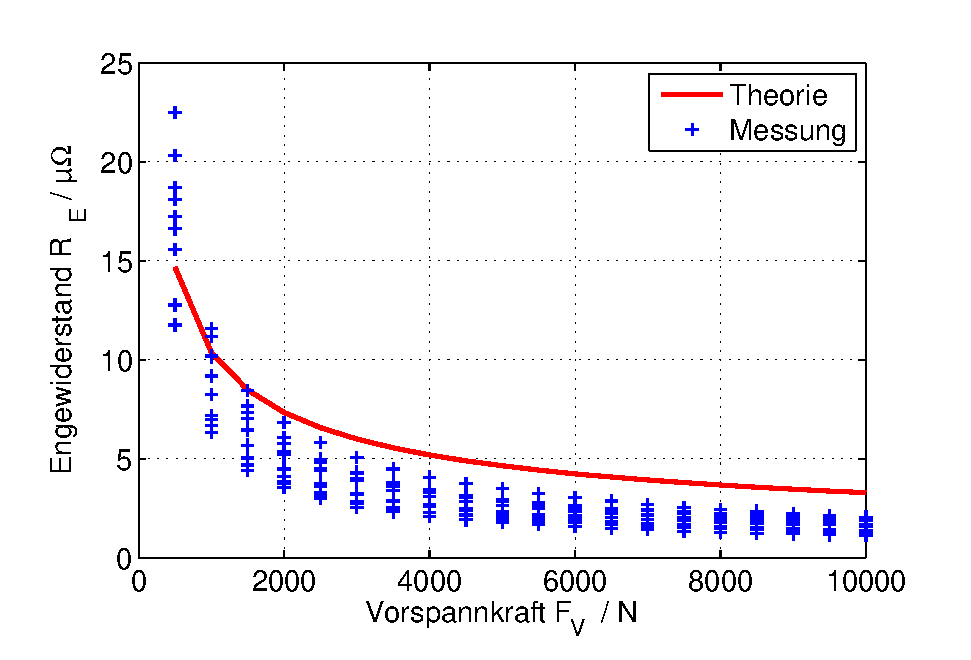
\includegraphics[width=0.5\textwidth]{Kapitel2/Bilder/image11}}
  \caption{Lineares zeitinvariantes System} 
  \label{fig:Zeitinvarianzsys}
\end{figure}

\noindent Für LTI-Systeme sind vergleichsweise anschauliche und einfach zu interpretierende Lösungs- und Interpretationsmethoden im Zeit- und Frequenzbereich vorhanden. Die Darstellungen in diesem Buch beschränken sich bis auf wenige Ausnahmen auf LTI-Systeme.\newline
Systeme, die mit einer linearen Differentialgleichung mit konstanten Koeffizienten beschrieben werden können, erfüllen die Bedingungen nach Linearität und Zeitinvarianz. Ausgehend von der allgemeinen Differentialgleichung

\begin{equation}\label{eq:threefourtyfive}
a_{0}\cdot y(t) + a_{1}\cdot \frac{dy}{dt}+a_{2}\cdot \frac{d^2y}{dt^2}+ ... +a_{n}\cdot \frac{d^Ny}{dt^N}=
b_{0}\cdot u(t) + b_{1}\cdot \frac{du}{dt}+b_{2}\cdot \frac{d^2u}{dt^2}+ ... +b_{m}\cdot \frac{d^Mu}{dt^M}
\end{equation}

\noindent beziehungsweise ihrer Darstellung als Summenformel

\begin{equation}\label{eq:threefourtysix}
\sum_{n=0}^{N}a_{n} \cdot  \frac{d^ny}{dt^n} =
\sum_{m=0}^{M}b_{m} \cdot  \frac{d^mu}{dt^m}
\end{equation}

\noindent werden die Eigenschaften der Linearität und Zeitinvarianz nachgewiesen.\bigskip

{\fontfamily{phv}\selectfont\noindent \textbf{Linearität}}\smallskip

\noindent Ausgangspunkt für den Beweis der Linearität sind zwei Signalkombinationen $u_{1}(t)$  und $y_{1}(t)$ sowie $u_{2}(t)$ und $y_{2}(t)$, für die gilt:

\begin{equation}\label{eq:threefourtyseven}
\sum_{n=0}^{N}a_{n} \cdot  \frac{d^ny_{1}}{dt^n} =
\sum_{m=0}^{M}b_{m} \cdot  \frac{d^mu_{1}}{dt^m}
\end{equation}

\begin{equation}\label{eq:threefourtyeight}
\sum_{n=0}^{N}a_{n} \cdot  \frac{d^ny_{2}}{dt^n} =
\sum_{m=0}^{M}b_{m} \cdot  \frac{d^mu_{1}}{dt^m}
\end{equation}

\noindent Ist das System linear, muss die Differentialgleichung bei einer Kombination von Eingangssignalen

\begin{equation}\label{eq:threefourtynine}
u(t)=v_{1}\cdot u_{1}(t)+v_{2}\cdot u_{2}(t)
\end{equation}

\noindent mit derselben Linearkombination der Ausgangssignale

\begin{equation}\label{eq:threefifty}
y(t)=v_{1}\cdot y_{1}(t)+v_{2}\cdot y_{2}(t)
\end{equation}

\noindent erfüllt sein. Einsetzen der Gleichungen führt zu

\begin{equation}\label{eq:threefiftyone}
\begin{split}
\sum _{n=0}^{N}a_{n} \cdot \frac{d^{n} y}{dt^{n} }   & = \sum _{n=0}^{N}a_{n} \cdot \frac{d^{n} \left(\nu _{1} \cdot y_{1} \left(t\right)+\nu _{2} \cdot y_{2} \left(t\right)\right)}{dt^{n} }  =\sum _{n=0}^{N}a_{n} \cdot \nu _{1} \cdot \frac{d^{n} y_{1} }{dt^{n} } +a_{n} \cdot \nu _{2} \cdot \frac{d^{n} y_{2} }{dt^{n} }  + \\ 
& =\nu _{1} \cdot \sum _{n=0}^{N}a_{n} \cdot \frac{d^{n} y_{1} }{dt^{n} }  +\nu _{2} \cdot \sum _{n=0}^{N}a_{n} \cdot \frac{d^{n} y_{2} }{dt^{n} }  =\nu _{1} \cdot \sum _{m=0}^{M}b_{m} \cdot \frac{d^{m} u_{1} }{dt^{m} }  +\nu _{2} \cdot \sum _{m=0}^{M}b_{m} \cdot \frac{d^{m} u_{2} }{dt^{m} }\\ 
& = \sum _{m=0}^{M}b_{m} \cdot \nu _{1}  \cdot \frac{d^{m} u_{1} }{dt^{m} } + b_{m} \nu _{2} \cdot \frac{d^{m} u_{2} }{dt^{m}} = \sum _{m=0}^{M}b_{m} \cdot \frac{d^{m} \left(\nu _{1} \cdot y_{1} \left(t\right)+\nu _{2} \cdot y_{2} \left(t\right)\right)}{dt^{m} }\\
& = \sum _{m=0}^{M}b_{m} \cdot \frac{d^{m}u}{dt^{m}}
\end{split}
\end{equation}

\noindent Eine Linearkombination von Eingangssignalen führt damit zu der identischen Linearkombination von Ausgangssignalen, sodass das System ein lineares System ist. \bigskip

{\fontfamily{phv}\selectfont
\noindent\textbf{Zeitinvarianz}}\smallskip

\noindent Das System wird mit einer Differentialgleichung mit konstanten Koeffizienten beschrieben. Damit ist das Systemverhalten von der Zeit unabhängig, und das System ist zeitinvariant.

\subsubsection{Kausalität}

\noindent Hängt das Ausgangssignal $y(t)$ eines Systems zu einem Zeitpunkt $t_{1}$ nur von Eingangswerten $u(t)$ mit $t \leqslant  t_{1}$ ab, wird das System als kausales System bezeichnet. Physikalisch sinnvolle und realisierbare Systeme sind wegen des Ursachewirkungsprinzips kausal.\bigskip

\noindent
\colorbox{lightgray}{%
\arrayrulecolor{white}%
\renewcommand\arraystretch{0.6}%
\begin{tabular}{ wl{16.5cm} }
Beispiel: Aufheizvorgang Wasserbad 
\end{tabular}%
}\bigskip

\noindent Aus der Erfahrung im Umgang mit Aufheizvorgängen ist bekannt, dass sich die Temperatur in einem Wasserbad erst dann erhöht, wenn eine Heizung eingeschaltet wird. Die Kausalität ergibt sich auch aus der mathematischen Beschreibung.

\begin{equation}\label{eq:threefiftytwo}
\frac{C_{TH}}{\alpha\cdot A} \cdot \frac{\Delta\vartheta(t)}{dt} + \Delta\vartheta(t) = \frac{p_{EL}(t)}{\alpha\cdot A}
\end{equation}

\noindent Erst wenn elektrische Leistung $p_{EL}(t)$ in das System eingespeist wird, ändert sich die Temperatur
$\Delta\vartheta(t)$.\bigskip

\noindent
\colorbox{lightgray}{%
\arrayrulecolor{white}%
\renewcommand\arraystretch{0.6}%
\begin{tabular}{ wl{16.5cm} }
Beispiel: Differenzierer als nicht kausales System
\end{tabular}%
}\bigskip

\noindent Die Differentiation eines Signals u(t) kann mathematisch beschrieben werden als

\begin{equation}\label{eq:threefiftythree}
y(t) = \frac{du}{dt} \approx \frac{u\left(t+\Delta t\right)-u\left(t-\Delta t\right)}{2\cdot \Delta t} 
\end{equation}

\noindent Zur Berechnung der Ableitung werden Eingangssignale verwendet, die in der Zukunft liegen. Ein Differenzierer ist damit kein kausales System.

\subsubsection{Stabilität}

Zur Erklärung des Begriffes der Stabilität wird von einem physikalischen Gedankenexperiment ausgegangen.
Eine Kugel liegt auf einer Fläche, die unterschiedliche Krümmungen aufweist. In allen Fällen liegt die Kugel zunächst in einer Ruhelage, die mit x = 0 bezeichnet wird. Die Kugel wird aus dieser Ruhelage um $x_{0}$  ausgelenkt und danach sich selber überlassen.

\begin{figure}[H]
  \centerline{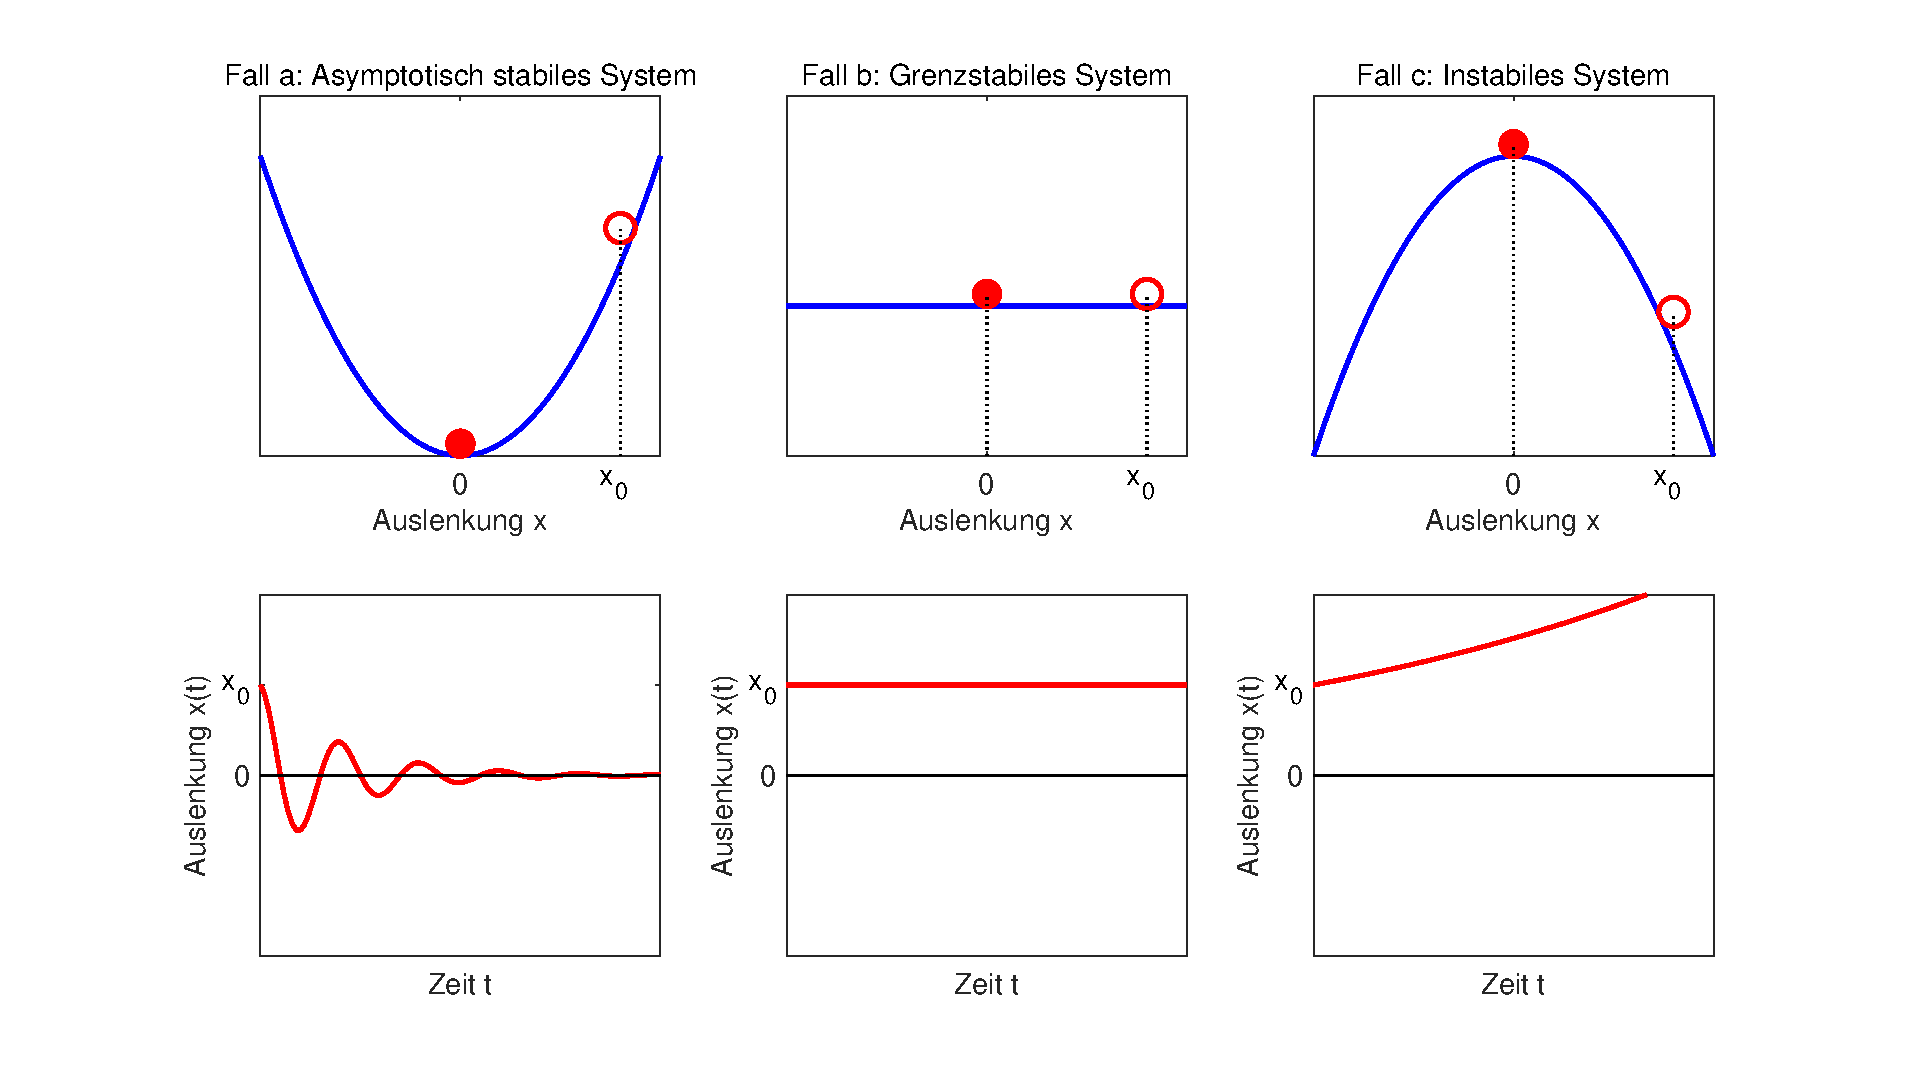
\includegraphics[width=1\textwidth]{Kapitel2/Bilder/image12}}
  \caption{Gedankenmodell zur Erklärung des Stabilitätsbegriffes}
  \label{fig:StabilitaetErklaerung}
\end{figure}

\noindent Im Fall a wirkt auf die Kugel nach der Auslenkung eine tangentiale Kraftkomponente, die sie in Richtung der Ruhelage beschleunigt. In der Stelle x = 0 wird die Kraftkomponente zu null, die Kugel besitzt jedoch eine Geschwindigkeit $v_{0}$  und überstreicht die Ruhelage. Lageenergie wird in kinetische
Energie gewandelt und umgekehrt. Aufgrund der Reibung und des Luftwiderstandes gibt die Kugel Energie an die Umgebung ab, die Auslenkung wird kleiner und schließlich gelangt die Kugel wieder
in die Ruhelage x = 0. Das System wird als asymptotisch stabil bezeichnet. Im Fall b wird die Kugel nach einer einmaligen Auslenkung $x_{0}$ dort liegen bleiben, da sie keine Kraft erfährt, die tangential auf sie wirkt. Da die Kugel nicht mehr in ihre Ruhelage zurückkehrt, ist das System nicht asymptotisch stabil, die Auslenkung der Kugel steigt aber auch nicht an. Das System wird deshalb als grenzstabil bezeichnet. Im Fall c wird die Kugel nach einer Auslenkung um $x_{0}$ die Fläche herunterrollen, mit steigender Auslenkung nimmt die tangentiale Kraftkomponente zu. Wegen der steigenden Auslenkung wird das System als instabil bezeichnet.\newline
Aus diesem Gedankenexperiment ergibt sich eine physikalische Stabilitätsdefinition: Ein System ist asymptotisch stabil, wenn es nach einer Anregung mit endlicher Energie wieder seine Ruheposition erreicht. Es ist grenzstabil, wenn es nach Anregung mit endlicher Energie zu einem konstanten Ausgangswert konvergiert, und es ist instabil, wenn es auf eine Anregung endlicher Energie mit divergierendem Ausgangssignal reagiert.\newline
Diese physikalische Stabilitätsdefinition ist zwar anschaulich, jedoch praktisch schlecht auszuwerten. Deshalb wird der Stabilitätsbegriff bei der Diskussion der charakteristischen Gleichung in Abschnitt \ref{threethreetwo} und des Faltungsintegrals in Abschnitt \ref{threefourfive} erneut aufgegriffen.

\subsubsection{Systeme mit und ohne Ausgleich}

\noindent Zur Interpretation von Systemen ist die Frage wichtig, ob das vorliegende System ein System mit oder ohne Ausgleich ist. Zur Einführung wird das Beispiel des Aufheizvorgangs aufgegriffen. Der Aufheizvorgang wird über die Differentialgleichung

\begin{equation}\label{eq:threefiftyfour}
p_{EL}(t) = C_{TH}\cdot \frac{\Delta\vartheta(t)}{dt}+ \alpha\cdot A \cdot \Delta\vartheta(t)
\end{equation}

\noindent beschrieben. Bei Einschalten des Tauchsieders wird elektrische Leistung $p_{EL}(t)$ in Wärme umgewandelt.
Es ergibt sich eine Temperaturerhöhung $\Delta\vartheta(t)$. Diese Temperaturerhöhung führt wiederum zu einer größeren Wärmeabgabe an die Umgebung. Es stellt sich ein stationärer Betriebspunkt ein. Er ist dadurch gekennzeichnet, dass die zugeführte und die abgeführte Wärme gleich groß sind. Mathematisch ergibt sich das stationäre Gleichgewicht dadurch, dass alle Ableitungen nach der Zeit zu null werden. Für den Aufheizprozess gilt in diesem Fall der Zusammenhang

\begin{equation}\label{eq:threefiftyfive}
p_{EL}(t) = C_{TH}\cdot 0 + \alpha\cdot A \cdot \Delta\vartheta(t) =\alpha\cdot A \cdot \Delta\vartheta(t)
\end{equation}

\noindent Allgemein wird ein System, das bei Anregung mit einem konstant begrenzten Eingangssignal mit einem konstant begrenzten Ausgangssignal reagiert, als System mit Ausgleich bezeichnet. Alle in Abschnitt \ref{threeone} diskutierten Systeme sind System mit Ausgleich. Generell findet ein Ausgleich statt, wenn ein Eingangssignal $u(t)$ durch ein Ausgangssignal $y(t)$ kompensiert wird. Dazu muss in der Differentialgleichung

\begin{equation}\label{eq:threefiftysix}
a_{0}\cdot y(t) + a_{1}\cdot \frac{dy}{dt}+a_{2}\cdot \frac{d^2y}{dt^2}+ ... +a_{n}\cdot \frac{d^Ny}{dt^N}=
b_{0}\cdot u(t) + b_{1}\cdot \frac{du}{dt}+b_{2}\cdot \frac{d^2u}{dt^2}+ ... +b_{m}\cdot \frac{d^Mu}{dt^M}
\end{equation}

\noindent die Bedingung $a_{0} \neq  0$  gelten. Wird bei Anregung des Systems mit konstant begrenztem Signal kein stationäres Gleichgewicht erreicht, handelt es sich um ein System ohne Ausgleich. Systeme mit integrierendem Verhalten wie bewegte Massen oder Flüssigkeitsbehälter sind Beispiele für Systeme ohne Ausgleich.\bigskip

\noindent
\colorbox{lightgray}{%
\arrayrulecolor{white}%
\renewcommand\arraystretch{0.6}%
\begin{tabular}{ wl{16.5cm} }
{\fontfamily{phv}\selectfont{Beispiel: System ohne Ausgleich}}
\end{tabular}%
}\bigskip

\noindent In Bild \ref{fig:SysohneAusgleich} ist ein zylindrischer Behälter der Grundfläche A ohne Auslauf dargestellt. In den Behälter fließt ein Volumenstrom Q(t). Bild \ref{fig:SysohneAusgleich} zeigt schematisch den Aufbau.

\begin{figure}[H]
  \centerline{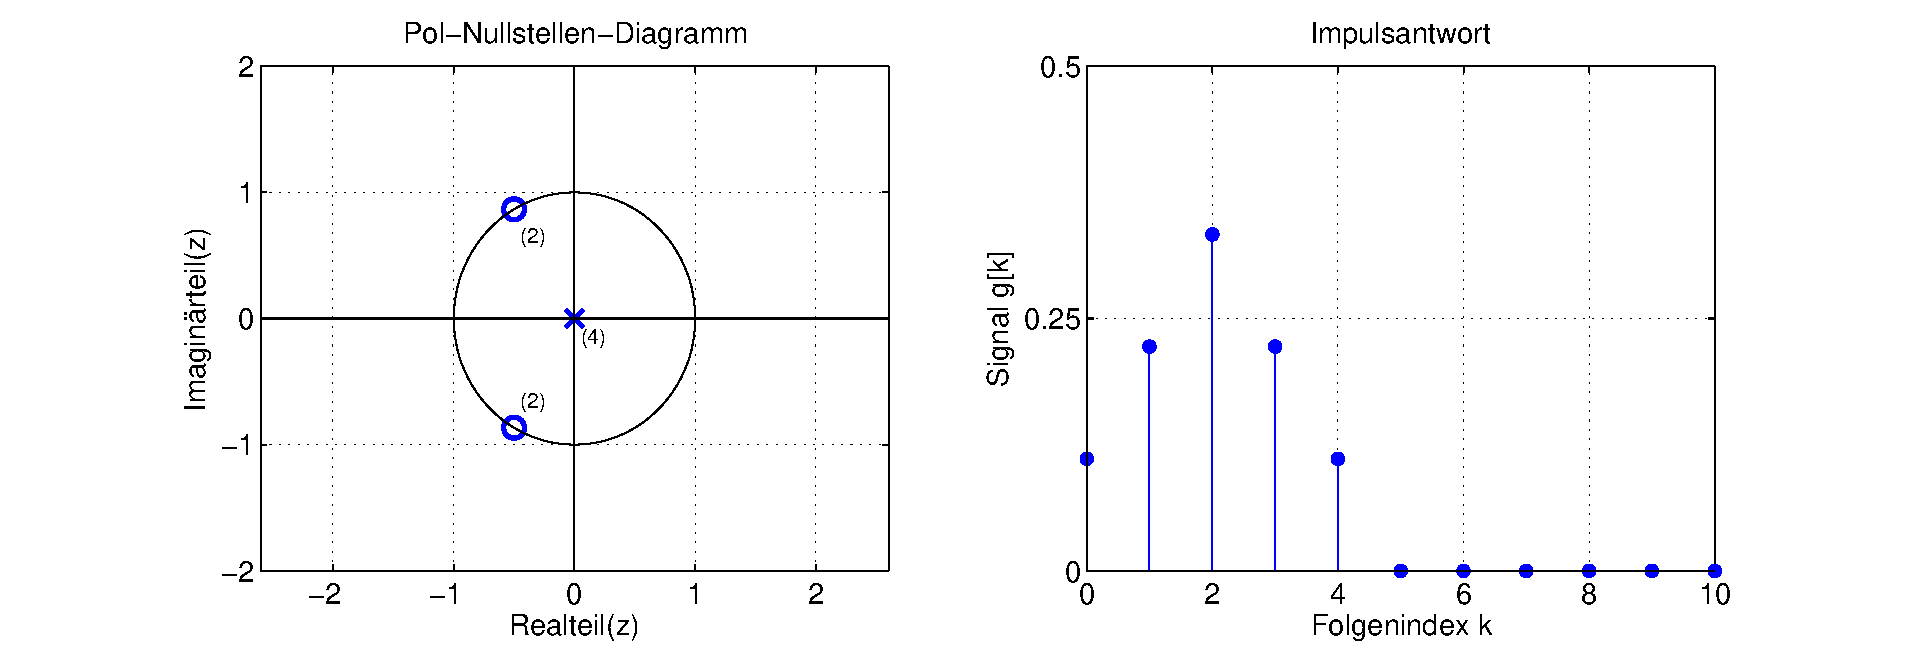
\includegraphics[width=0.5\textwidth]{Kapitel2/Bilder/image13}}
  \caption{Behälter ohne Auslauf als Beispiel für ein System ohne Ausgleich}
  \label{fig:SysohneAusgleich}
\end{figure}

\noindent Die Füllstandshöhe h(t) wird über die Gleichung


\begin{equation}\label{eq:fiftyseven}
x(t)=\frac{1}{A}\cdot\int\limits _{0}^{t}Q(\tau)d\tau+X_{0}
\end{equation}

\noindent beschrieben. Ableiten von Gleichung (\ref{eq:fiftyseven}) führt zu der Differentialgleichung

\begin{equation}\label{eq:fiftyeight}
0\cdot x(t) + \frac{dx}{dt}=\frac{1}{A}\cdot Q(t)
\end{equation}

\noindent Es existiert kein stationäres Gleichgewicht, da im stationären Gleichgewicht die Ableitung dh/dt zu null würde. Gleichung (\ref{eq:fiftyeight}) kann in diesem Fall nicht erfüllt werden, da der Koeffizient $a_{0}=0$ ist. Gleichung (\ref{eq:fiftyseven}) zeigt, dass die Füllstandshöhe h kontinuierlich ansteigt. Das Systemverhalten ist in Bild \ref{fig:Behaelter}  für eine Querschnittsfläche $A=10m^2$ und einen Anfangszustand $x_{0}=2m$ dargestellt.

\begin{figure}[H]
  \centerline{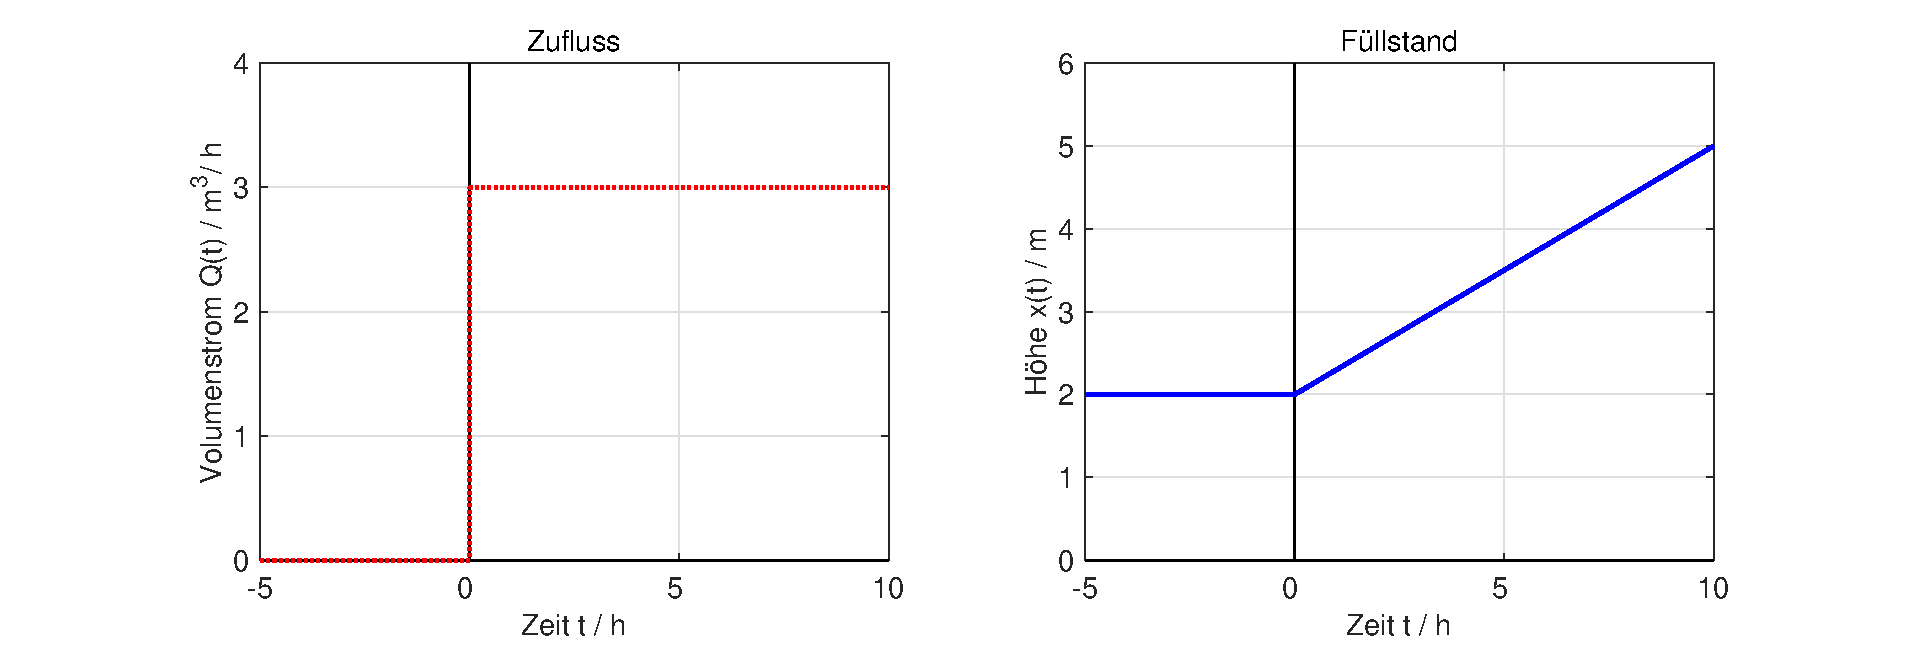
\includegraphics[width=1\textwidth]{Kapitel2/Bilder/image14}}
  \caption{Anregung eines Tanks ohne Auslauf mit einem konstanten Volumenstrom}
  \label{fig:Behaelter}
\end{figure}

\noindent Ein Volumenstrom $Q(t) > 0$ führt zu einem Anstieg der Füllstandshöhe. Es findet kein Ausgleich statt. Es handelt sich demnach um ein System ohne Ausgleich.

\clearpage

\subsubsection{Zusammenfassung grundlegender Systemeigenschaften}

Tabelle \ref{tab:threefour} fasst die diskutierten Systemeigenschaften und ihre Bedeutung zusammen.

\begin{table}[H]
\caption{Zusammenfassung von Systemeigenschaften und ihrer Bedeutung}
\setlength{\fboxsep}{0pt}%
\colorbox{lightgray}{%
\arrayrulecolor{white}%
\begin{tabular}{| c | c |}
\hline
\parbox[c][0.28in][c]{3.3in}{\smallskip\centering\textbf{\fontfamily{phv}\selectfont{Eigenschaft}}} & \parbox[c][0.28in][c]{3.3in}{\smallskip\centering\textbf{\fontfamily{phv}\selectfont{Bedeutung}}}\\ \hline

\parbox[c][1.2in][c]{3.3in}{\centering{\fontfamily{phv}\selectfont{Linearität}}} &
\parbox[c][1.2in][c]{3.3in}{\centering{\fontfamily{phv}\selectfont{System reagiert auf Linearkombination von Eingangssignale  \\
$u(t)=v_{1}\cdot u_{1}(t)+v_{2}\cdot u_{2}(t)$\\
mit derselben Linearkombination von Ausgangssignalen\\
$y(t)=v_{1}\cdot y_{1}(t)+v_{2}\cdot y_{2}(t)$}}}\\ \hline

\parbox[c][0.64in][c]{3.3in}{\centering{\fontfamily{phv}\selectfont{Zeitinvarianz}}} & \parbox[c][0.64in][c]{3.3in}{\centering{\fontfamily{phv}\selectfont{System reagiert auf ein verzögertes\\
Eingangssignal $u(t - t_{0})$\\
mit einem Ausgangsignal $y(t - t_{0})$}}}\\ \hline

\parbox[c][0.64in][c]{3.3in}{\centering{\fontfamily{phv}\selectfont{Kausalität}}} &
\parbox[c][0.64in][c]{3.3in}{\centering{\fontfamily{phv}\selectfont{System reagiert auf ein Eingangssignal\\
erst nach Beginn der Anregung}}}\\ \hline

\parbox[c][0.64in][c]{3.3in}{\centering{\fontfamily{phv}\selectfont{Asymptotische Stabilität}}} & 
\parbox[c][0.64in][c]{3.3in}{\centering{\fontfamily{phv}\selectfont{System erreicht nach einer Anregung\\
mit endlicher Energie\\
wieder seine Ruheposition}}}\\ \hline

\parbox[c][0.64in][c]{3.3in}{\centering{\fontfamily{phv}\selectfont{Grenzstabilität}}} & 
\parbox[c][0.64in][c]{3.3in}{\centering{\fontfamily{phv}\selectfont{System bleibt nach einer Anregung\\
mit endlicher Energie\\
in dem aktuellen Zustand}}}\\ \hline

\parbox[c][0.8in][c]{3.3in}{\centering{\fontfamily{phv}\selectfont{Instabilität}}} & 
\parbox[c][0.8in][c]{3.3in}{\centering{\fontfamily{phv}\selectfont{System reagiert nach einer Anregung mit endlicherEnergie mit einer divergierenden Systemantwort}}}\\ \hline

\parbox[c][0.64in][c]{3.3in}{\centering{\fontfamily{phv}\selectfont{System mit Ausgleich}}} & 
\parbox[c][0.64in][c]{3.3in}{\centering{\fontfamily{phv}\selectfont{Differentialgleichung mit dem Koeffizienten\\
$a_{0}\neq 0$}}}\\ \hline

\end{tabular}%
}
\label{tab:threefour}
\end{table}

\clearpage

\subsection{Lösung linearer Differentialgleichungen mit konstanten Koeffizienten}\label{threethree}
Zur Charakterisierung von Systemen werden oftmals Sprung- und Impulsantworten verwendet. Sie lassen sich bei linearen, zeitinvarianten Systemen im Zeitbereich mit der Vier-Schritt-Methode berechnen.

\subsubsection{Lösung von Anfangswertproblemen mit der Vier-Schritt-Methode}
Bei technischen Anwendungen werden lineare, zeitinvariante Systeme durch lineare Differentialgleichungen mit konstanten Koeffizienten beschrieben.

\begin{equation}\label{eq:fiftynine}
a_{0}\cdot y(t) + a_{1}\cdot \frac{dy}{dt}+a_{2}\cdot \frac{d^2y}{dt^2}+ ... +a_{n}\cdot \frac{d^Ny}{dt^N}=
b_{0}\cdot u(t) + b_{1}\cdot \frac{du}{dt}+b_{2}\cdot \frac{d^2u}{dt^2}+ ... +b_{m}\cdot \frac{d^Mu}{dt^M}
\end{equation}

\noindent Zur Charakterisierung dieser Systeme kann das Einschwingverhalten y(t) unter Berücksichtigung von Anfangswerten des Signals y(t = 0) bestimmt werden. Diese Aufgabenstellungen werden in der Mathematik als Anfangswertprobleme bezeichnet. Die Lösung dieser Anfangswertprobleme erfolgt mit der Vier-Schritt-Methode. Grundlage für das Lösungsverfahren ist, zunächst alle sogenannten homogenen Lösungen der Differentialgleichung zu finden und sie dann mit einer sogenannten partikulären Lösung zu kombinieren. Aus der Menge dieser Lösungen wird abschließend diejenige ausgewählt, die die Anfangsbedingungen der Aufgabenstellung erfüllt. Die Vier-Schritt-Methode umfasst damit folgende Schritte:

\begin{itemize}
  \item Berechnung der allgemeinen homogenen Lösungen
  \item Berechnung einer partikulären Lösung
  \item Superposition von homogener und partikulärer Lösung
  \item Bestimmung der Konstanten über Anfangsbedingungen
\end{itemize}

\noindent Eine ausführliche Darstellung der Vier-Schritt-Methode mit unterschiedlichen Lösungsvarianten ist in [Papu11] und [Goeb11] zu finden. Hier wird eine Lösungsmöglichkeit beschrieben und am Beispiel des RC-Netzwerks angewendet.\bigskip

{\fontfamily{phv}\selectfont
\noindent\textbf{Berechnung der allgemeinen homogenen Lösungen}}\smallskip

\noindent Die lineare Differentialgleichung mit konstanten Koeffizienten (\ref{eq:fiftynine}) beschreibt den Zusammenhang
zwischen Eingangssignal u(t) und Ausgangssignal y(t). Zur Bestimmung der homogenen Differentialgleichungen wird das Eingangssignal u(t) zu null gesetzt.

\begin{equation}\label{eq:sixty}
a_{0}\cdot y_{H}(t) + a_{1}\cdot \frac{dy_{H}}{dt}+a_{2}\cdot \frac{d^2y_{H}}{dt^2}+ ... +a_{n}\cdot \frac{d^Ny_{H}}{dt^N}=
0
\end{equation}

\noindent Die Gleichung besteht aus einer mit den Koeffizienten an gewichteter Summe der Funktion $y_{H}(t)$ und ihren Ableitungen. Zur Lösung dieser Gleichung wird eine Exponentialfunktion angesetzt.

\begin{equation}\label{eq:sixtyone}
y_{H}(t) + Y_{0}\cdot e^{\lambda \cdot t}
\end{equation}

\noindent Sie hat die Eigenschaft, dass ihre Ableitungen selbst wieder Exponentialfunktionen sind.

\begin{equation}\label{eq:sixtytwo}
\frac{d^n y_{H}}{dt^n}= \lambda ^n \cdot e^{\lambda \cdot t}
\end{equation}

\noindent Durch Einsetzen in die homogene Differentialgleichung ergibt sich die Gleichung

\begin{equation}\label{eq:sixtythree}
\begin{split}
0 & = a_{0} \cdot y_{H} \left(t\right)+a_{1} \cdot \frac{dy_{H} }{dt} +a_{2} \cdot \frac{d^{2} y_{H} }{dt^{2} } +...+a_{N} \cdot \frac{d^{N} y_{H} }{dt^{N} }\\ \medskip
& = a_{0} \cdot Y_{0}\cdot e^{\lambda \cdot t} + a_{1}\cdot\lambda \cdot Y_{1}\cdot e^{\lambda \cdot t} + a_{2}\cdot\lambda ^2 \cdot Y_{2}\cdot e^{\lambda \cdot t} +...+ a_{N}\cdot\lambda ^N \cdot Y_{N}\cdot e^{\lambda \cdot t}\\\medskip
& = (a_{0} + a_{1}\cdot\lambda + a_{2}\cdot\lambda ^2 + ... + a_{N}\cdot\lambda ^N) \cdot Y_{0} \cdot e^{\lambda\cdot t}
\end{split}
\end{equation}

\noindent Die Gleichung ist für $Y_{0} = 0$  erfüllt. Dieser Fall ist jedoch technisch weniger von Interesse, da er den Ruhezustand des Systems beschreibt. Für $Y_{0} \neq 0$ kann die Gleichung vereinfacht werden zu

\begin{equation}\label{eq:sixtyfour}
0 = a_{0}+a_{1}\cdot \lambda + a_{2}\cdot \lambda ^2 +...+a_{N}\cdot \lambda ^N
\end{equation}

\noindent Mit der Gleichung werden die Werte $\lambda _{n}$ bestimmt, für die die Exponentialfunktion die vorliegende homogene Differentialgleichung löst. Die Gleichung wird deshalb auch charakteristische Gleichung des Systems genannt. Ein Polynom N-ter Ordnung weist N Nullstellen auf, sodass die Nullstellen
$\lambda _{1} ... \lambda _{N}$ Lösungen der charakteristischen Gleichung sind. Es kann gezeigt werden, dass sich die allgemeine Lösung der homogenen Differentialgleichung $y_{H}(t)$ bei einfachen Nullstellen $\lambda _{n}$ aus der Linearkombination

\begin{equation}\label{eq:sixtyfive}
y_{H} \left(t\right)=Y_{1} \cdot e^{\lambda _{1} \cdot t} +Y_{2} \cdot e^{\lambda _{2} \cdot t} +...+Y_{N} \cdot e^{\lambda _{N} \cdot t} 
\end{equation}

\noindent ergibt [Goeb11]. Die Lösungen der charakteristischen Gleichung müssen jedoch nicht die Vielfachheit von eins haben. Existiert eine P-fache Nullstelle $\lambda _{1}$, ergibt sich die homogene Lösung

\begin{equation}\label{eq:sixtysix}
y_{H} \left(t\right)=Y_{1} \cdot e^{\lambda _{1} \cdot t} +Y_{2} \cdot t\cdot e^{\lambda _{1} \cdot t} +...+Y_{P} \cdot t^{P-1} \cdot e^{\lambda _{1} \cdot t} +Y_{P+1} \cdot e^{\lambda _{2} \cdot t} +Y_{P+2} \cdot e^{\lambda _{3} \cdot t} +...+Y_{N} \cdot e^{\lambda _{N-P+1} \cdot t}
\end{equation}

\noindent
\colorbox{lightgray}{%
\arrayrulecolor{white}%
\renewcommand\arraystretch{0.6}%
\begin{tabular}{ wl{16.5cm} }
{\smallskip{\fontfamily{phv}\selectfont{
Beispiel: Einschwingverhalten eines RC-Netzwerks}}} 
\end{tabular}%
}\bigskip

\noindent Als Beispiel wird das Einschaltverhalten des RC-Netzwerks aus Bild \ref{fig:RCSchaltbild} berechnet. Die Ausgangsspannung des RC-Netzwerks wird über die Differentialgleichung

\begin{equation}\label{eq:sixtyseven}
R \cdot C \cdot\frac{dU_{A}}{dt} + U_{A}(t) =U_{E}(t) 
\end{equation}

\noindent beschrieben. Die zugehörige homogene Differentialgleichung lautet

\begin{equation}\label{eq:sixtyeight}
R \cdot C \cdot\frac{dU_{AH}}{dt} + U_{AH}(t) =0
\end{equation}

\noindent Einsetzen der Exponentialfunktion

\begin{equation}\label{eq:sixtynine}
 u_{AH}(t)= U_{H} \cdot e^{\lambda \cdot t}
\end{equation}

\noindent führt mit $U_{H} \neq 0$ zu der charakteristischen Gleichung

\begin{equation}\label{eq:seventy}
 0=U_{AH}(t)= R \cdot C \cdot \lambda U_{H} \cdot e^{\lambda \cdot t}+U_{H} \cdot e^{\lambda \cdot t}= (R \cdot C \cdot \lambda +1)\cdot U_{H} \cdot e^{\lambda \cdot t}
\end{equation}

\noindent mit der Lösung 

\begin{equation}\label{eq:seventyone}
\lambda=-\frac{1}{R\cdot C}
\end{equation}

\noindent Damit ergibt sich die Lösung der homogenen Differentialgleichung zu

\begin{equation}\label{eq:seventytwo}
u_{AH}(t) = U_{H} \cdot e^{-\frac{1}{R\cdot C}\cdot t}
\end{equation}

\noindent Die Konstante $U_{H}$ ist zunächst unbekannt, sie wird später über die Anfangsbedingungen des Systems bestimmt.\medskip

{\fontfamily{phv}\selectfont
\noindent\textbf{Berechnung einer partikulären Lösung}} \smallskip

\noindent Im zweiten Schritt wird eine partikuläre oder spezielle Lösung der Differentialgleichung bestimmt. Dabei wird von der Differentialgleichung

\begin{equation}\label{eq:seventythree}
a_{0}\cdot y(t) + a_{1}\cdot \frac{dy}{dt}+a_{2}\cdot \frac{d^2y}{dt^2}+ ... +a_{n}\cdot \frac{d^Ny}{dt^N}=
b_{0}\cdot u(t) + b_{1}\cdot \frac{du}{dt}+b_{2}\cdot \frac{d^2u}{dt^2}+ ... +b_{m}\cdot \frac{d^Mu}{dt^M}
\end{equation}

\noindent mit $u(t) \neq 0$ ausgegangen, und es wird für $t\geqslant  0$ eine Lösung gesucht. Wesentlich ist, dass eine beliebige partikuläre Lösung ausreicht, da sie durch Kombination mit der allgemeinen homogenen Lösung das Anfangswertproblem beschreibt.
Eine partikuläre Lösung der Differentialgleichung kann auf verschiedene Arten bestimmt werden [Goeb11]. Hier wird die Lösung durch Lösungsansätze vorgestellt. Die Lösungsansätze sind im Allgemeinen von der Ordnung der Differentialgleichung abhängig und können in [Papu01] oder [Goeb11] nachgeschlagen werden. Für die hier relevanten Fälle einer konstanten Anregung oder einer harmonischen Anregung sind die Lösungsansätze jedoch von der Ordnung der Differentialgleichung unabhängig. Sie sind in Tabelle \ref{tab:threefive} zusammengefasst.

\begin{table}[H]
\caption{Lösungsansätze für die partielle Lösung linearer Differentialgleichungen mit konstanten Koeffizienten}
\setlength{\fboxsep}{0pt}%
\colorbox{lightgray}{%
\arrayrulecolor{white}%
\begin{tabular}{| c | c |}
\hline
\parbox[c][0.28in][c]{3.3in}{\smallskip\centering\textbf{\fontfamily{phv}\selectfont{Eingangssignal u(t) für $t \geqslant 0$}}} & \parbox[c][0.28in][c]{3.3in}{\smallskip\centering\textbf{\fontfamily{phv}\selectfont{Lösungsansatz y$_{p}(t)$}}}\\ \hline

\parbox[c][0.64in][c]{3.3in}{\centering{\fontfamily{phv}\selectfont{Konstantes Eingangssignal\\
u(t) = U}}} &
\parbox[c][0.64in][c]{3.3in}{\centering{\fontfamily{phv}\selectfont{Konstantes Ausgangssignal\\
y$_{P}$(t) = Y}}}\\ \hline

\parbox[c][1in][c]{3.3in}{\centering{\fontfamily{phv}\selectfont{Harmonisches Eingangssignal\\
u(t) = U $\cdot$ cos($\omega t + \mu _{x}$)}}} & \parbox[c][1in][c]{3.3in}{\centering{\fontfamily{phv}\selectfont{Harmonisches Ausgangssignal\\
y$_{P}$(t) = Y $\cdot$ cos($\omega t + \mu _{y}$)\\
wenn $j\cdot\omega$ keine Lösung\\
der charakteristischen Gleichung ist}}}\\ \hline

\parbox[c][1in][c]{3.3in}{\centering{\fontfamily{phv}\selectfont{Exponentielles Eingangssigna\\
u(t) = U $\cdot$ e$^{c\cdot x}$}}} &
\parbox[c][1in][c]{3.3in}{\centering{\fontfamily{phv}\selectfont{Exponentielles Ausgangssignal\\
y$_{P}$(t) = Y$\cdot$ e$^{c\cdot x}$\\
wenn c keine Lösung \\ der charakteristischen Gleichung ist}}}\\ \hline

\end{tabular}%
}
\label{tab:threefive}
\end{table}

\noindent Die freien Parameter des Lösungsansatzes ergeben sich aus dem vorliegenden Eingangssignal sowie
der vorliegenden Differentialgleichung. Dies wird am einfachsten an einem konkreten Beispiel deutlich.\bigskip

\noindent
\colorbox{lightgray}{%
\arrayrulecolor{white}%
\renewcommand\arraystretch{0.6}%
\begin{tabular}{ wl{16.5cm} }
{\fontfamily{phv}\selectfont{
Beispiel: Einschwingverhalten eines RC-Netzwerks}}
\end{tabular}%
}\bigskip

\noindent Zur Berechnung der Systemreaktion auf ein konstantes Eingangssignal der Größe $U_{E0}$ wird für $t \geqslant 0$ das Eingangssignal

\begin{equation}\label{eq:seventyfour}
u_{E} \left(t\right)=U_{E0} 
\end{equation}

\noindent in die Differentialgleichung eingesetzt.

\begin{equation}\label{eq:seventyfive}
R\cdot C\cdot \frac{du_{AP} }{dt} +u_{AP} \left(t\right)=U_{E0} 
\end{equation}

\noindent Der Ansatz für die partikuläre Lösung bei einer konstanten Anregung ist wieder eine Konstante. 

\begin{equation}\label{eq:seventysix}
u_{AP} \left(t\right)=U_{A0}
\end{equation}

\noindent Ihre Ableitung ist null. Einsetzen in die Differentialgleichung führt zu

\begin{equation}\label{eq:seventyseven}
R\cdot C\cdot 0+U_{A0} =U_{E0}
\end{equation}

\noindent Die beiden Konstanten U$_{E0}$ und U$_{A0}$ sind demnach identisch, sodass die partikuläre Lösung für t $\geq$ 0 lautet:

\begin{equation}\label{eq:seventyeight}
u_{AP} \left(t\right)=U_{E0}
\end{equation}

\noindent Das hier vorgestellte Verfahren führt zu einem stetigen Ausgangssignal. Es versagt, wenn das Ausgangssignal Sprünge oder Impulse aufweist. Für die korrekte Berechnung der Systemantwort muss in dem Fall eine sogenannte Übergangsbedingung berücksichtigt werden. Das entsprechende Verfahren wird in Abschnitt 3.3.2 beschrieben..\bigskip

{\fontfamily{phv}\selectfont
\noindent\textbf{Superposition von homogener und partikulärer Lösung}}\smallskip

\noindent Sind die allgemeine homogene Lösung und eine partikuläre Lösung bekannt, ergibt sich die Lösung der Differentialgleichung aus deren Summe.

\begin{equation}\label{eq:seventynine}
y\left(t\right)=y_{H} \left(t\right)+y_{P} \left(t\right)
\end{equation}

\noindent Dabei weist die homogene Lösung noch unbekannte Parameter auf, die später über Anfangsbedingungen
zu bestimmen sind.\bigskip

\noindent
\colorbox{lightgray}{%
\arrayrulecolor{white}%
\renewcommand\arraystretch{0.6}%
\begin{tabular}{ wl{16.5cm} }
{\fontfamily{phv}\selectfont{
Beispiel: Einschwingverhalten eines RC-Netzwerks}}
\end{tabular}%
}\bigskip

\noindent Bei dem Einschaltverhalten eines RC-Netzwerks ergibt sich die Lösung aus der Summe von homogener Lösung

\begin{equation}\label{eq:eighty}
u_{AH} \left(t\right)=U_{H} \cdot e^{-\frac{1}{R\cdot C} \cdot t}
\end{equation}

\noindent und partikulärer Lösung

\begin{equation}\label{eq:eightyone}
u_{AP} \left(t\right)=U_{E0} 
\end{equation}

\noindent zu

\begin{equation}\label{eq:eightytwo}
u_{A} \left(t\right)=U_{H} \cdot e^{-\frac{1}{R\cdot C} \cdot t} +U_{E0}
\end{equation}

\noindent Dabei ist die Konstante U$_{H}$ noch unbekannt.\bigskip

{\fontfamily{phv}\selectfont
\noindent\textbf{Bestimmung der Konstanten über Anfangsbedingungen}}\smallskip

\noindent Die Summe aus homogener und partikulärer Lösung weist Parameter auf, die bestimmt werden müssen. Es kann gezeigt werden, dass bei einer Differentialgleichung N-ter Ordnung N Parameter zu bestimmen sind. Dazu werden N Bedingungen benötigt. Bei Anfangswertproblemen sind diese Bedingungen
die Anfangswerte der Funktion y(t) und ihrer N - 1 Ableitungen an der Stelle t = 0.\bigskip

\noindent
\colorbox{lightgray}{%
\arrayrulecolor{white}%
\renewcommand\arraystretch{0.6}%
\begin{tabular}{ wl{16.5cm} }
{\fontfamily{phv}\selectfont{
Beispiel: Einschwingverhalten eines RC-Netzwerks}}
\end{tabular}%
}\bigskip

\noindent Bei dem RC-Netzwerk handelt es sich um ein System, das mit einer Differentialgleichung erster Ordnung beschrieben wird. Die allgemeine Lösung lautet

\begin{equation}\label{eq:eightythree}
u_{A} \left(t\right)=U_{H} \cdot e^{-\frac{1}{R\cdot C} \cdot t} +U_{E0}
\end{equation}

\noindent Zur Bestimmung des Parameters U${}_{H}$ wird die Ausgangsspannung u${}_{A}$(0) verwendet. Es ergibt sich

\begin{equation}\label{eq:eightyfour}
u_{A} \left(0\right)=U_{H} \cdot e^{-\frac{1}{R\cdot C} \cdot 0} +U_{E0} =U_{H} +U_{E0}
\end{equation}

\noindent beziehungsweise

\begin{equation}\label{eq:eightyfive}
U_{H} =u_{A} \left(0\right)-U_{E0}
\end{equation}

\noindent Daraus ergibt sich die Lösung des Anfangswertproblems in Abhängigkeit der Ausgangsspannung u$_{A}$(0) zum Zeitpunkt t = 0 zu

\begin{equation}\label{eq:eightysix}
u_{A} \left(t\right)=\left(u_{A} \left(0\right)-U_{E0} \right)\cdot e^{-\frac{1}{R\cdot C} \cdot t} +U_{E0} =u_{A} \left(0\right)\cdot e^{-\frac{1}{R\cdot C} \cdot t} +U_{E0} \cdot \left(1-e^{-\frac{1}{R\cdot C} \cdot t} \right)
\end{equation}

\noindent Die Ausgangsspannung setzt sich aus zwei Termen zusammen. Der erste Term beschreibt das Abklingen der Anfangsbedingung, der zweite Term beschreibt die Reaktion des Systems auf einen Spannungssprung am Eingang. Bild \ref{fig:RCEinschwingenAnfangsbedingungen} zeigt das Einschwingverhalten der Kondensatorspannung u$_{A}$(t) für eine Spannung U$_{E0}$ = 5 V, einen Widerstand von 5 k$\Omega$ und eine Kapazität von 4 nF bei unterschiedlichen
Anfangswerten.

\begin{figure}[H]
  \centerline{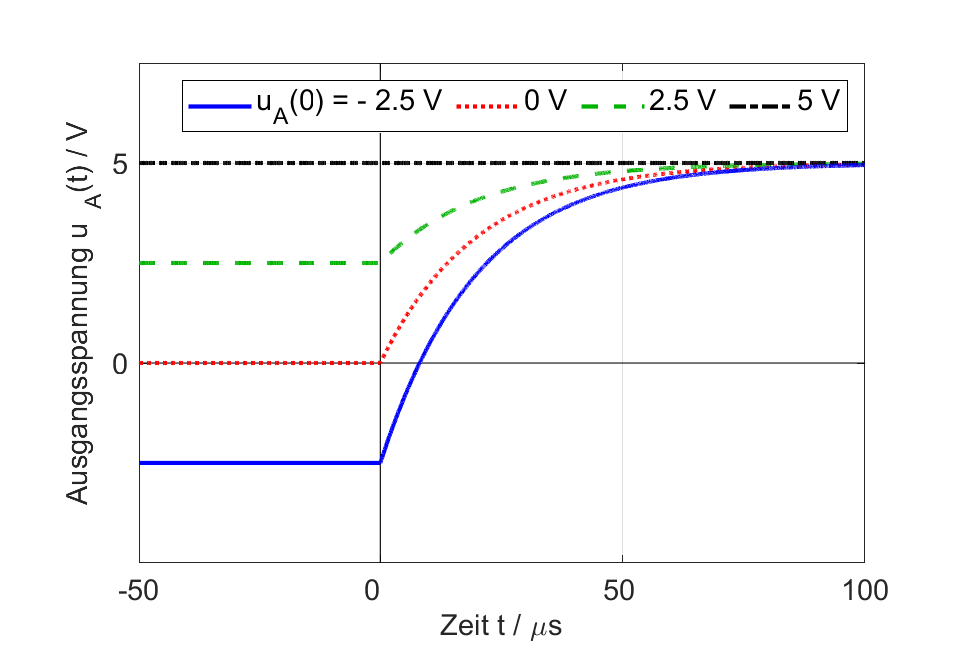
\includegraphics[width=0.5\textwidth]{Kapitel2/Bilder/image15}}
  \caption{Einschwingverhalten der Kondensator Spannung u${}_{A}$(t) bei Anregung mit einem Spannungssprung von 5 V und verschiedenen Anfangsbedingungen u${}_{A}$(0)}
  \label{fig:RCEinschwingenAnfangsbedingungen}
\end{figure}

\noindent Das Ausgangssignal schwingt abhängig von dem Anfangswert auf den Endwert von u$_{A}$ = 5 V ein.\bigskip
\clearpage

{\fontfamily{phv}\selectfont
\noindent\textbf{Zusammenfassung}}\smallskip

\noindent Das Vorgehen bei der Vierschrittmethode zur Lösung linearer Differentialgleichungen mit konstanten Koeffizienten ist in Tabelle \ref{tab:threesix} zusammengefasst.

\begin{table}[H]
\caption{Lösungsansätze für die partielle Lösung linearer Differentialgleichungen mit konstanten Koeffizienten}
\setlength{\fboxsep}{0pt}%
\colorbox{lightgray}{%
\arrayrulecolor{white}%
\begin{tabular}{| c | c |}
\hline
\parbox[c][0.28in][c]{0.45in}{\smallskip\centering\textbf{\fontfamily{phv}\selectfont{Schritt}}} & \parbox[c][0.28in][c]{6in}{\smallskip\centering\textbf{\fontfamily{phv}\selectfont{Beschreibung}}}\\ \hline

\parbox[c][2in][c]{0.45in}{\centering{1}} &
\parbox[c][2in][c]{6in}{\centering{\fontfamily{phv}\selectfont{
Lösung der homogenen Differentialgleichung\\
$a_{0} \cdot y_{H} \left(t\right)+a_{1} \cdot \frac{dy_{H} }{dt} +a_{2} \cdot \frac{d^{2} y_{H} }{dt^{2} } +...+a_{N} \cdot \frac{d^{N} y_{H} }{dt^{N} } =0$ \\ 
über Ansatz\\
$y_{H} \left(t\right)=Y_{0} \cdot e^{\lambda \cdot t} $\newline 
durch Lösen der charakteristischen Gleichung\\
$0=a_{0} +a_{1} \cdot \lambda +a_{2} \cdot \lambda ^{2} +...+a_{N} \cdot \lambda ^{N} $\\
Allgemeine Lösung in Abhängigkeit der Vielfachheit\\ 
$y_{H} \left(t\right)=Y_{1} \cdot e^{\lambda _{1} \cdot t} +Y_{2} \cdot t\cdot e^{\lambda _{1} \cdot t} +...+Y_{P} \cdot t^{P-1} \cdot e^{\lambda _{1} \cdot t} +Y_{P+1} \cdot e^{\lambda _{2} \cdot t} +Y_{P+2} \cdot e^{\lambda _{3} \cdot t} +...+Y_{N} \cdot e^{\lambda _{N-P+1} \cdot t} $

}}}\\ \hline

\parbox[c][0.5in][c]{0.45in}{\centering{2}} & \parbox[c][0.5in][c]{6in}{\centering{\fontfamily{phv}\selectfont{Bestimmung einer partikulären Lösung y${}_{p}$(t) über einen Lösungsansatz je nach Eingangssignal}}}\\ \hline

\parbox[c][0.5in][c]{0.45in}{\centering{3}} &
\parbox[c][0.5in][c]{6in}{\centering {\fontfamily{phv}\selectfont{Superposition von allgemeiner homogener und partikulärer Lösung\\ 
$y\left(t\right)=y_{H} \left(t\right)+y_{P} \left(t\right)$}}}\\ \hline

\parbox[c][0.4in][c]{0.45in}{\centering{4}} &
\parbox[c][0.4in][c]{6in}{\centering{\fontfamily{phv}\selectfont{Bestimmung der unbekannten Konstanten über Anfangsbedingungen}}}\\ \hline

\end{tabular}%
}\bigskip
\label{tab:threesix}
\end{table}

\subsubsection{Exkurs zu Übergangsbedingungen bei linearen Differentialgleichungen}\label{threethreetwo}

\noindent Die in Abschnitt 3.3.1 beschriebene Vier-Schritt-Methode eignet sich zur Lösung linearer Differentialgleichung, bei denen das Ausgangssignal stetig ist. Deshalb wird die Vier-Schritt-Methode stufenweise ergänzt, um Sprünge oder allgemein Singularitäten berücksichtigen zu können.\bigskip

{\fontfamily{phv}\selectfont
\noindent\textbf{Lösung linearer Differentialgleichungen bei stetigem Ausgangssignal (N $\boldsymbol{\mathrm{>}}$ P)}}

\noindent Ist das Ausgangssignal stetig, sind rechter und linker Grenzwert an der Stelle t = 0 identisch.

\begin{equation}\label{eq:eightyseven}
y\left(0_{+} \right)=y\left(0_{-} \right)
\end{equation}

\noindent Die Rechnung erfolgt in diesem Fall wie in Abschnitt 3.3.1. Zur Überleitung wird dieser Fall noch einmal aufgegriffen und hinsichtlich der Anfangsbedingung intensiver interpretiert.\bigskip

\noindent
\colorbox{lightgray}{%
\arrayrulecolor{white}%
\renewcommand\arraystretch{0.6}%
\begin{tabular}{ wl{16.5cm} }
{\fontfamily{phv}\selectfont{
Beispiel: Lineare Differentialgleichung und stetiges Ausgangssignal}}
\end{tabular}%
}\bigskip

\noindent Als einführendes Beispiel wird das Ausgangssignal für ein System mit der Differentialgleichung

\begin{equation}\label{eq:eightyeight}
\frac{dy}{dt} +6\cdot y\left(t\right)=u\left(t\right)
\end{equation}

\noindent berechnet. Das Eingangssignal ist 

\begin{equation}\label{eq:eightynine}
\frac{dy}{dt} +6\cdot y\left(t\right)=u\left(t\right)
\end{equation}

\noindent und die Anfangsbedingung lautet y(0${}_{-}$) = U${}_{1}$. Zur Berechnung des Ausgangssignals y(t) wird zunächst für t $\mathrm{>}$ 0 die homogene Differentialgleichung 

\begin{equation}\label{eq:ninety}
\frac{dy_{H} }{dt} +6\cdot y_{H} \left(t\right)=0
\end{equation}

\noindent mit dem Ansatz

\begin{equation}\label{eq:ninetyone}
y_{H} \left(t\right)=Y_{H} \cdot e^{\lambda \cdot t} \cdot \sigma \left(t\right)
\end{equation}

\noindent gelöst. Für t $\mathrm{>}$ 0 ergibt sich über durch Einsetzen 

\begin{equation}\label{eq:ninetytwo}
\lambda \cdot Y_{H} \cdot e^{\lambda \cdot t} +6\cdot Y_{H} \cdot e^{\lambda \cdot t} =0
\end{equation}

\noindent die charakteristische Gleichung

\begin{equation}\label{eq:ninetythree}
\lambda +6=0
\end{equation}

\noindent Sie besitzt die Lösung $\lambda$ = - 6. Damit lautet für t $\mathrm{>}$ 0 die allgemeine homogene Lösung

\begin{equation}\label{eq:ninetyfour}
y_{H} \left(t\right)=Y_{H} \cdot e^{-6\cdot t} \cdot \sigma \left(t\right)
\end{equation}

\noindent Da das Eingangssignal für t $\mathrm{>}$ 0 konstant ist, ist die Konstante y${}_{P}$(t) = Y${}_{P}$ eine partikuläre Lösung. Einsetzen in die Differentialgleichung führt zu

\begin{equation}\label{eq:ninetyfive}
0+6\cdot Y_{P} =U_{0} 
\end{equation}

\noindent beziehungsweise

\begin{equation}\label{eq:ninetysix}
Y_{P} =\frac{1}{6} \cdot U_{0}
\end{equation}

\noindent Damit lautet die L\"{o}sung der Differentialgleichung

\begin{equation}\label{eq:ninetyseven}
y\left(t\right)=y_{H} \left(t\right)+y_{P} \left(t\right)=\left(Y_{H} \cdot e^{-6\cdot t} +\frac{1}{6} \cdot U_{0} \right)\cdot \sigma \left(t\right)
\end{equation}

\noindent Das Eingangssignal u(t) ist an der Stelle t = 0 nicht stetig, es springt. Um die Differentialgleichung 

\begin{equation}\label{eq:ninetyeight}
\frac{dy}{dt} +6\cdot y\left(t\right)=u\left(t\right)
\end{equation}

\noindent erfüllen zu können, muss auch das Ausgangssignal y(t) oder eine Ableitung des Ausgangssignals springen. $\frac{dy}{dt} +6\cdot y\left(t\right)=u\left(t\right)$W\"{u}rde y(t) springen, wäre dy/dt ein Impuls. Dieser Impuls hat kein entsprechendes Pendant auf der Eingangsseite. Deshalb muss dy/dt an der Stelle t = 0 springen. Das Signal y(t) ist damit an der Stelle t = 0 stetig und springt nicht. 

\begin{equation}\label{eq:ninetynine}
y\left(0_{+} \right)=y\left(0_{-} \right)=U_{1}
\end{equation}

\noindent Mit diesen Anfangswerten wird die Unbekannte Y${}_{H}$ bestimmt. 

\begin{equation}\label{eq:hundred}
y\left(0_{+} \right)=Y_{H} +\frac{1}{6} \cdot U_{0} =U_{1} 
\end{equation}

\noindent Die Konstante Y${}_{H}$ errechnet sich zu

\begin{equation}\label{eq:hundredone}
Y_{H} =U_{1} -\frac{1}{6} \cdot U_{0} 
\end{equation}

\noindent Damit lautet die Lösung der Differentialgleichung für t $\mathrm{>}$ 0 

\begin{equation}\label{eq:hundredtwo}
y\left(t\right)=\left(\left(U_{1} -\frac{1}{6} \cdot U_{0} \right)\cdot e^{-6\cdot t} +\frac{1}{6} \cdot U_{0} \right)\cdot \sigma \left(t\right)
\end{equation}

\noindent Liegt bei dem Eingangssignal u(t) ein Sprung an der Stelle t = 0 vor, führt diese Unstetigkeit in Kombination mit einer Ableitung du/dt des Eingangssignals zu einem Impuls an der Stelle t = 0. Damit kann die Aufgabenstellung mit der in Abschnitt 3.3.1 beschriebenen Vier-Schritt-Methode alleine nicht gelöst werden. Auch bei höheren Ableitungen des Eingangssignals u(t) in Kombination mit unstetigen Eingangssignalen versagt die Vier-Schritt-Methode. Ein impulsförmiges Eingangssignal u(t) = $\delta$(t) führt ebenfalls zu einer Aufgabenstellung, die mit der Vier-Schritt-Methode alleine nicht gelöst werden kann. 

\begin{equation}\label{eq:hundredthree}
\frac{d\delta }{dt} =\frac{d^{2} \sigma }{dt^{2} }
\end{equation}

\noindent die Ordnung P = 2 auf. Um eine Differentialgleichung für Eingangssignale mit Singularitäten zu lösen, müssen auf beiden Seiten der Differentialgleichung alle Ordnungen der Singularitäten dasselbe Gewicht haben. $a_{n} \cdot \frac{d^{n} y}{dt^{n} } =\sum _{m=0}^{M}b_{m} \cdot \frac{d^{m} u}{dt^{m} }  $In dem Beispiel oben hat diese Abschätzung dazu geführt, dass das Ausgangssignal y(t) stetig ist. Auch bei der Differentialgleichung 

\begin{equation}\label{eq:hundredfour}
\frac{d^{2} y}{dt^{2} } +5\cdot \frac{dy}{dt} +6\cdot y\left(t\right)=\frac{du}{dt}
\end{equation}

\noindent und einem Eingangssignal 

\begin{equation}\label{eq:hundredfive}
u\left(t\right)=U_{0} \cdot \sigma \left(t\right)
\end{equation}

\noindent wäre das Ausgangssignal stetig. Das Eingangssignal weist unter Berücksichtigung der Ableitung eine Singularität der Ordnung P = 1 auf. Deshalb muss die zweite Ableitung von y(t) einen Impuls aufweisen und die erste Ableitung einen Sprung besitzen. Damit ist y(t) stetig. Dieser Ansatz führt deshalb immer dann zum Ergebnis, wenn die Ordnung N der Differentialgleichung grö{\ss}er ist als die Ordnung P der Singularit\"{a}t.

\begin{equation}\label{eq:hundredsix}
N>P
\end{equation}\medskip

{\fontfamily{phv}\selectfont
\noindent\textbf{Lösung linearer Differentialgleichungen bei springendem Ausgangssignal (N = P)}}

\noindent Sind die Ordnungen der Differentialgleichung N und der Singularität P gleich gro{\ss}, weist das Ausgangssignal einen Sprung auf. Die Anfangsbedingung y(0-) ist deshalb nicht identisch zu y(0+) und kann nicht zur Bestimmung der Konstante in der homogenen Lösung verwendet werden. Zur Lösung dieser Aufgabenstellungen wird deshalb eine Übergangsbedingung benötigt, die das Verhalten an der Stelle t = 0 beschreibt. Dazu wird die Lösung y(t) in einen linken Bereich (t $\mathrm{<}$ 0) und einen rechten Bereich (t $\mathrm{>}$ 0) aufgeteilt. 

\begin{equation}\label{eq:hundredseven}
y\left(t\right)=y_{L} \left(t\right)\cdot \sigma \left(-t\right)+y_{R} \left(t\right)\cdot \sigma \left(t\right)
\end{equation}

\noindent Zwischen den beiden Bereichen findet der Sprung des Ausgangsignals statt, der mit Hilfe der Ausblendeigenschaft der Impulsfunktion bestimmt wird. Das Vorgehen wird wieder an einem Beispiel beschrieben.\bigskip

\noindent
\colorbox{lightgray}{%
\arrayrulecolor{white}%
\renewcommand\arraystretch{0.6}%
\begin{tabular}{ wl{16.5cm} }
{\fontfamily{phv}\selectfont{
Beispiel: Lineare Differentialgleichung und stetiges Ausgangssignal}}
\end{tabular}%
}\bigskip

\noindent Um zu untersuchen, wie Differentialgleichungen mit springendem Ausgangssignal berechnet werden, wird die Differentialgleichung

\begin{equation}\label{eq:hundredeight}
\frac{dy}{dt} +6\cdot y\left(t\right)=\frac{du}{dt}
\end{equation}

\noindent bei einem Eingangssignal 

\begin{equation}\label{eq:hundrednine}
u\left(t\right)=U_{0} \cdot \sigma \left(t\right)
\end{equation}

\noindent und der Anfangsbedingung y(0${}_{-}$) = U${}_{1}$ betrachtet. Auf der rechten Seite wird der Sprung am Eingang abgeleitet, es liegt also eine Singularit\"{a}t erster Ordnung (P = 1) vor. Die h\"{o}chste Ableitung auf der linken Seite ist die erste Ableitung des Ausgangssignals (N =1). Um der Singularit\"{a}t auf der rechten Seite zu entsprechen, muss das Ausgangssignal y(t) einen Sprung aufweisen. Es gibt f\"{u}r das Ausgangssignal also eine L\"{o}sung y${}_{R}$(t) f\"{u}r t $\mathrm{>}$ 0 und eine L\"{o}sung y${}_{L}$(t) f\"{u}r t $\mathrm{<}$ 0. 

\begin{equation}\label{eq:hundredten}
y\left(t\right)=y_{L} \left(t\right)\cdot \sigma \left(-t\right)+y_{R} \left(t\right)\cdot \sigma \left(t\right)
\end{equation}

\noindent Formell berechnet sich die erste Ableitung zu

\begin{equation}\label{eq:hundredeleven}
\begin{split}
\frac{dy}{dt}  & = -y_{L} \left(t\right)\cdot \delta \left(-t\right)+\frac{dy_{L} }{dt} \cdot \sigma \left(-t\right)+y_{R} \left(t\right)\cdot \delta \left(t\right)+\frac{dy_{R} }{dt} \cdot \sigma \left(t\right) \\ 
& = \frac{dy_{R} }{dt} \cdot \sigma \left(t\right)+\frac{dy_{L} }{dt} \cdot \sigma \left(-t\right)+\left(y_{R} \left(t\right)-y_{L} \left(t\right)\right)\cdot \delta \left(t\right)  
\end{split}
\end{equation}

\noindent Einsetzen in die Differentialgleichung führt zu

\begin{equation}\label{eq:hundredtwelve}
\frac{dy_{R} }{dt} \cdot \sigma \left(t\right)+\frac{dy_{L} }{dt} \cdot \sigma \left(-t\right)+\left(y_{R} \left(t\right)-y_{L} \left(t\right)\right)\cdot \delta \left(t\right)+6\cdot \left(y_{L} \left(t\right)\cdot \sigma \left(-t\right)+y_{R} \left(t\right)\cdot \sigma \left(t\right)\right)=\frac{du}{dt}
\end{equation}

\noindent F\"{u}r die \"{U}bergangsbedingung ist nur das Verhalten an der Stelle t = 0 relevant. Zur Berechnung der \"{U}bergangsbedingung wird davon ausgegangen, dass die L\"{o}sungen f\"{u}r t $\mathrm{<}$ 0 und t $\mathrm{>}$ 0 existieren.

\begin{equation}\label{eq:hundredthirteen}
\frac{dy_{L} }{dt} +6\cdot y_{L} \left(t\right)=0
\end{equation}

\begin{equation}\label{eq:hundredfourteen}
\frac{dy_{R} }{dt} +6\cdot y_{R} \left(t\right)=0
\end{equation}

\noindent Damit kann Gleichung \eqref{eq:hundredtwelve} vereinfacht werden zu

\begin{equation}\label{eq:hundredfifteen}
\left(y_{R} \left(t\right)-y_{L} \left(t\right)\right)\cdot \delta \left(t\right)=\frac{du}{dt} =U_{0} \cdot \delta \left(t\right)
\end{equation}

\noindent Integrieren der Gleichung 

\begin{equation}\label{eq:hundredsixteen}
\int\limits _{-\infty }^{\infty }\left(y_{R} \left(t\right)-y_{L} \left(t\right)\right)\cdot \delta \left(t\right)\, \, dt =\int\limits _{-\infty }^{\infty }U_{0} \cdot \delta \left(t\right)\, \, dt
\end{equation}

\noindent f\"{u}hrt mit der Ausblendeigenschaft der Impulsfunktion zu 

\begin{equation}\label{eq:hundredseventeen}
y_{R} \left(0\right)-y_{L} \left(0\right)=U_{0}
\end{equation}

\noindent Damit lautet der rechtseitige Anfangswert 

\begin{equation}\label{eq:hundredeighteen}
y\left(0_{+} \right)=y_{R} \left(0\right)=U_{0} +y_{L} \left(0\right)=U_{0} +y\left(0_{-} \right)=U_{0} +U_{1} 
\end{equation}

\noindent An der L\"{o}sung der homogenen Differentialgleichung f\"{u}r t $\mathrm{>}$ 0 \"{a}ndert sich nichts.

\begin{equation}\label{eq:hundrednineteen}
y_{H} \left(t\right)=Y_{H} \cdot e^{-6\cdot t} \cdot \sigma \left(t\right)
\end{equation}

\noindent Da das Eingangssignal u${}_{E}$(t) = U${}_{0}$ f\"{u}r t $\mathrm{>}$ 0 konstant ist, ist die Ableitung null und y${}_{P}$(t) = 0 ist eine partikul\"{a}re L\"{o}sung. Damit lautet die L\"{o}sung der Differentialgleichung

\begin{equation}\label{eq:hundredtwenty}
y\left(t\right)=y_{H} \left(t\right)+y_{P} \left(t\right)=Y_{H} \cdot e^{-6\cdot t} \cdot \sigma \left(t\right)+0=Y_{H} \cdot e^{-6\cdot t} \cdot \sigma \left(t\right)
\end{equation}

\noindent Die Konstante Y${}_{H}$ wird \"{u}ber den berechneten Anfangswert bestimmt 

\begin{equation}\label{eq:hundredtwentyone}
Y_{H} =y\left(0_{+} \right)=U_{0} +U_{1}
\end{equation}

\noindent und die L\"{o}sung der Differentialgleichung lautet 

\begin{equation}\label{eq:hundredtwentytwo}
y\left(t\right)=\left(U_{0} +U_{1} \right)\cdot e^{-6\cdot t} \cdot \sigma \left(t\right)
\end{equation}

\noindent Sie springt erwartungsgem\"{a}{\ss} an der Stelle t = 0. \bigskip

{\fontfamily{phv}\selectfont
\noindent\textbf{Lösung linearer Differentialgleichungen mit impulsförmigen Ausgangssignal (N $\boldsymbol{\mathrm{<}}$ P)}}

\noindent Ist die Ordnung der Differentialgleichung N kleiner als die Ordnung der Singularit\"{a}t P, kann das Ausgangssignal einen Impuls und Ableitungen davon aufweisen. Wie bei dem Beispiel mit N = P muss die Anfangsbedingung y(0${}_{-}$) nicht identisch zu y(0${}_{+}$) sein. Zus\"{a}tzlich sind bei der L\"{o}sung ein Impuls an der Stelle t = 0 und seine Ableitungen mit unbekanntem Gewicht zu ber\"{u}cksichtigen. Je h\"{o}her die Differenz der Singularit\"{a}t P im Vergleich zur Ordnung der Differentialgleichung ist, desto h\"{o}here Ableitungen der Impulse sind zu ber\"{u}cksichtigen. Im Allgemeinen lautet damit die L\"{o}sung der Differentialgleichung

\begin{equation}\label{eq:hundredtwentythree}
y\left(t\right)=y_{L} \left(t\right)\cdot \sigma \left(-t\right)+y_{R} \left(t\right)\cdot \sigma \left(t\right)+\sum _{p=0}^{P-N-1}Y_{p} \cdot \frac{d^{p} \delta }{dt^{p}} 
\end{equation}

\noindent Zur Bestimmung der Hilfe der Gewichte Yp und der Sprungh\"{o}he an der Stelle t = 0 wird auf Eigenschaften der Impulsfunktion zur\"{u}ckgegriffen, wie das folgende Beispiel zeigt.\bigskip

\noindent
\colorbox{lightgray}{%
\arrayrulecolor{white}%
\renewcommand\arraystretch{0.6}%
\begin{tabular}{ wl{16.5cm} }
{\fontfamily{phv}\selectfont{
Beispiel: Lineare Differentialgleichung und stetiges Ausgangssignal}}
\end{tabular}%
}\bigskip

\noindent Ausgangspunkt ist wie bei den Beispielen oben eine Differentialgleichung erster Ordnung.

\begin{equation}\label{eq:hundredtwentyfour}
\frac{dy}{dt} +6\cdot y\left(t\right)=\frac{du}{dt}
\end{equation}

\noindent Das Eingangssignal ist in diesem Beispiel

\begin{equation}\label{eq:hundredtwentyfive}
u\left(t\right)=U_{0} \cdot \delta \left(t\right)
\end{equation}

\noindent und die Anfangsbedingung ist wieder y(0${}_{-}$) = U${}_{1}$. 

\noindent Auf der rechten Seite wird der Impuls am Eingang abgeleitet, es liegt also eine Singularit\"{a}t zweiter Ordnung (P = 2) vor. Die h\"{o}chste Ableitung auf der linken Seite ist die erste Ableitung des Ausgangssignals (N =1). Um der Singularit\"{a}t auf der rechten Seite zu entsprechen, muss das Ausgangssignal y(t) einen Impuls aufweisen. Das Ausgangssignal setzt sich nach Gleichung \eqref{eq:hundredtwentythree} damit zusammen aus einer L\"{o}sung y${}_{R}$(t) f\"{u}r t $\mathrm{>}$ 0, einer L\"{o}sung y${}_{L}$(t) f\"{u}r t $\mathrm{<}$ 0 und einem Impuls mit unbekanntem Gewicht an der Stelle t = 0.

\begin{equation}\label{eq:threehundredtwentysix}
y\left(t\right)=y_{L} \left(t\right)\cdot \sigma \left(-t\right)+y_{R} \left(t\right)\cdot \sigma \left(t\right)+Y_{0} \cdot \delta \left(t\right)
\end{equation}

\noindent Formell berechnet sich die erste Ableitung zu

\begin{equation}\label{eq:threehundredtwentyseven}
\begin{split}
\frac{dy}{dt}  & = -y_{L} \left(t\right)\cdot \delta \left(-t\right)+\frac{dy_{L} }{dt} \cdot \sigma \left(-t\right)+y_{R} \left(t\right)\cdot \delta \left(t\right)+\frac{dy_{R} }{dt} \cdot \sigma \left(t\right)+Y_{0} \cdot \frac{d\delta }{dt}\\ 
& = \frac{dy_{R} }{dt} \cdot \sigma \left(t\right)+\frac{dy_{L} }{dt} \cdot \sigma \left(-t\right)+\left(y_{R} \left(t\right)-y_{L} \left(t\right)\right)\cdot \delta \left(t\right)+Y_{0} \cdot \frac{d\delta }{dt}
\end{split}
\end{equation}

\noindent Einsetzen in die Differentialgleichung f\"{u}hrt zu

\begin{equation}\label{eq:threehundredtwentyeight}
\begin{split}
\frac{du}{dt} & = \frac{dy_{R} }{dt} \cdot \sigma \left(t\right)+\frac{dy_{L} }{dt} \cdot \sigma \left(-t\right)+\left(y_{R} \left(t\right)-y_{L} \left(t\right)\right)\cdot \delta \left(t\right)+Y_{0} \cdot \frac{d\delta }{dt}\\ 
& +6\cdot \left(y_{L} \left(t\right)\cdot \sigma \left(-t\right)+y_{R} \left(t\right)\cdot \sigma \left(t\right)+Y_{0} \cdot \delta \left(t\right)\right)
\end{split}
\end{equation}

\noindent F\"{u}r die \"{U}bergangsbedingung ist nur das Verhalten an der Stelle t = 0 relevant. Wieder wird davon ausgegangen, dass die L\"{o}sungen f\"{u}r t $\mathrm{<}$ 0 und t $\mathrm{>}$ 0 existieren. 

\begin{equation}\label{eq:threehundredtwentynine}
\frac{dy_{L} }{dt} +6\cdot y_{L} \left(t\right)=0
\end{equation}

\begin{equation}\label{eq:threehundredthirty}
\frac{dy_{R} }{dt} +6\cdot y_{R} \left(t\right)=0
\end{equation}

\noindent Damit kann Gleichung \eqref{eq:threehundredtwentyeight} vereinfacht werden zu

\begin{equation}\label{eq:hundredthirtyone}
\left(y_{R} \left(t\right)-y_{L} \left(t\right)\right)\cdot \delta \left(t\right)+Y_{0} \cdot \frac{d\delta }{dt} +6\cdot Y_{0} \cdot \delta \left(t\right)=\frac{du}{dt} =U_{0} \cdot \frac{d\delta }{dt}
\end{equation}

\noindent Da in der Gleichung sowohl ein Impuls als auch seine Ableitung vorkommt, kann die Ausblendeigenschaft nicht alleine zur Aufl\"{o}sung genutzt werden Stattdessen wird die Gleichung \eqref{eq:hundredthirtyone} mit einer Funktion f(t) multipliziert und integriert. 

\begin{equation}\label{eq:threehundredthirtytwo}
\int\limits _{0_{-} }^{0_{+} }\left(\left(y_{R} \left(t\right)-y_{L} \left(t\right)\right)\cdot \delta \left(t\right)+Y_{0} \cdot \frac{d\delta }{dt} +6\cdot Y_{0} \cdot \delta \left(t\right)\right)\cdot f\left(t\right)\, \, dt =\int\limits  _{0_{-} }^{0_{+} }U_{0} \cdot \frac{d\delta }{dt} \cdot f\left(t\right)\, \, dt 
\end{equation}

\noindent Mit Hilfe der partiellen Integration kann das Integral \"{u}ber die Ableitung der Impulsfunktion umgerechnet werden. 

\begin{equation}\label{eq:threehundredthirtythree}
\int\limits  _{0_{-} }^{0_{+} }\frac{d\delta }{dt} \cdot x\left(t\right)\, \, dt =\delta \left(0_{+} \right)\cdot x\left(0_{+} \right)-\delta \left(0_{-} \right)\cdot x\left(0_{-} \right)-\int\limits  _{0_{-} }^{0_{+} }\delta \left(t\right)\cdot \frac{dx}{dt} \, \, dt
\end{equation}

\noindent Da die Impulsfunktion nur an der Stelle t = 0 von null verschieden ist, gilt mit der Ausblendeigenschaft der Impulsfunktion

\begin{equation}\label{eq:threehundredthirtyfour}
\int\limits _{0_{-} }^{0_{+} }\frac{d\delta }{dt} \cdot x\left(t\right)\, \, dt =-\left. \frac{dx}{dt} \right|_{t=0}
\end{equation}

\noindent Wird dieses Verfahren in Kombination mit der Ausblendeigenschaft auf Gleichung \eqref{eq:threehundredthirtyfive} angewendet, ergibt sich

\begin{equation}\label{eq:threehundredthirtyfive}
\left(y_{R} \left(0\right)-y_{L} \left(0\right)\right)\cdot f\left(0\right)-Y_{0} \cdot \left. \frac{df}{dt} \right|_{t=0} +6\cdot Y_{0} \cdot f\left(0\right)=-U_{0} \cdot \left. \frac{df}{dt} \right|_{t=0}
\end{equation}

\noindent Um diese Gleichung f\"{u}r beliebige Funktion f(t) zu erf\"{u}llen, m\"{u}ssen die Koeffizienten von f(0) und df/dt an der Stelle t = 0 \"{u}bereinstimmen. Es ergeben sich als zwei Gleichungen f\"{u}r zwei Unbekannte.

\begin{equation}\label{eq:threehundredthirtysix}
\left(y_{R} \left(0\right)-y_{L} \left(0\right)\right)+6\cdot Y_{0} =0
\end{equation}

\begin{equation}\label{eq:threehundredthirtyseven}
-Y_{0} =-U_{0}
\end{equation}

\noindent Damit ist Y${}_{0}$ = U${}_{0}$ und de Angangswert y(0${}_{+}$) berechnet sich zu

\begin{equation}\label{eq:threehundredthirtyeight}
y\left(0_{+} \right)=y_{R} \left(0\right)=y_{L} \left(0\right)-6\cdot Y_{0} =y\left(0_{-} \right)-6\cdot Y_{0} =U_{1} -6\cdot U_{0}
\end{equation}

\noindent An der L\"{o}sung der homogenen Differentialgleichung f\"{u}r t $\mathrm{>}$ 0 \"{a}ndert sich nichts. 

\begin{equation}\label{eq:threehundredthirtynine}
y_{H} \left(t\right)=Y_{H} \cdot e^{-6\cdot t} \cdot \sigma \left(t\right)
\end{equation}

\noindent Da das Eingangsignal u${}_{E}$(t) f\"{u}r t $\mathrm{>}$ 0 null ist, ist y${}_{P}$(t) = 0 ist eine partikul\"{a}re L\"{o}sung. Damit lautet die L\"{o}sung der Differentialgleichung

\begin{equation}\label{eq:threehundredfourty}
y\left(t\right)=y_{H} \left(t\right)+y_{P} \left(t\right)+Y_{0} \cdot \delta \left(t\right)=Y_{H} \cdot e^{-6\cdot t} \cdot \sigma \left(t\right)+0+U_{0} \cdot \delta \left(t\right)
\end{equation}

\noindent Die Konstante Y${}_{H}$ wird \"{u}ber die oben bestimmte Anfangsbedingungen bestimmt. 

\begin{equation}\label{eq:threehundredfourtyone}
y\left(0_{+} \right)=U_{1} -6\cdot U_{0} =Y_{H} \cdot e^{-6\cdot t} 
\end{equation}

\noindent Damit lautet die L\"{o}sung

\begin{equation}\label{eq:threehundredfourtytwo}
y\left(t\right)=\left(U_{1} -6\cdot U_{0} \right)\cdot e^{-6\cdot t} \cdot \sigma \left(t\right)+U_{0} \cdot \delta \left(t\right)
\end{equation}\bigskip

\noindent Das Verfahren wird in den Beispielen oben mit der \"{U}bersicht halber mit Differentialgleichungen erster Ordnung durchgef\"{u}hrt. Anhand eines komplexeren Beispiels wird in \"{U}bungsaufgabe 3.10 gezeigt, dass das Verfahren auch f\"{u}r Systeme h\"{o}herer Ordnung verwendet werden kann. \newline
Die Beispiel verdeutlichen, wie die \"{U}bergangsbedingungen f\"{u}r die Berechnung der Konstanten in der allgemeinem L\"{o}sung der Differentialglichung genutzt wird. Weiterf\"{u}hrende Literatur ist in [Bart89] zu finden.

\subsubsection{Stabilität und charakteristische Gleichung eines Systems}

Bei der Einf\"{u}hrung des Begriffes der Stabilit\"{a}t in Abschnitt 3.2.3 wird gezeigt, dass stabile Systeme nach einer Anregung mit endlicher Energie wieder in ihren Ausgangszustand zur\"{u}ckkehren. Das Verhalten des Systems nach der Anregung wird durch die homogene L\"{o}sung der Differentialgleichung beschrieben, die in Abschnitt 3.3.1 berechnet wird. Sie setzt sich bei einfachen Nullstellen $\lambda_{n}$ aus einer Linearkombination von Exponentialfunktionen zusammen. 

\begin{equation}\label{eq:threehundredfourtythree}
y_{H} \left(t\right)=Y_{1} \cdot e^{\lambda _{1} \cdot t} +Y_{2} \cdot e^{\lambda _{2} \cdot t} +...+Y_{N} \cdot e^{\lambda _{N} \cdot t} 
\end{equation}

\noindent Damit die homogene L\"{o}sung f\"{u}r t $\rightarrow$ $\infty$ zu null wird, m\"{u}ssen die Nullstellen $\lambda_{n}$ einen Realteil Re($\lambda_{n}$) $\mathrm{<}$ 0 aufweisen. Besitzt ein Wert $\lambda_{n}$ einen positiven Realteil, divergiert der entsprechende Summand aus Gleichung \eqref{eq:threehundredfourtythree}. Folglich divergiert auch die L\"{o}sung der homogenen Differentialgleichung. \newline
Liegt mit $\lambda_{1}$ eine P-fache L\"{o}sung der charakteristischen Gleichung vor, weisen die zugeh\"{o}rigen Summanden der homogenen L\"{o}sung Terme der Form

\begin{equation}\label{eq:threehundredfourtyfour}
y_{H} \left(t\right)=Y_{1} \cdot e^{\lambda _{1} \cdot t} +Y_{2} \cdot t\cdot e^{\lambda _{1} \cdot t} +...+Y_{P} \cdot t^{P-1} \cdot e^{\lambda _{1} \cdot t}
\end{equation}

\noindent auf. Da die Exponentialfunktion schneller f\"{a}llt und w\"{a}chst als jede Potenz von t, konvergiert diese Summe ebenfalls f\"{u}r einen negativen Realteil Re($\lambda_{1}$) $\mathrm{<}$ 0. Sie divergiert f\"{u}r einen positiven Realteil Re($\lambda_{1}$) $\mathrm{>}$ 0. Dabei ist es unerheblich, ob die L\"{o}sungen $\lambda_{n}$ reell oder komplex sind.\newline
Einen Sonderfall stellen L\"{o}sungen mit einem Realteil Re($\lambda_{n}$) = 0 dar.

\begin{equation}\label{eq:threehundredfourtyfive}
\begin{split}
y_{H} \left(t\right) & = Y_{1} \cdot e^{0\cdot t} +Y_{2} \cdot e^{\left(0+j\cdot \omega _{0} \right)\cdot t} +Y_{3} \cdot e^{\left(0-j\cdot \omega _{0} \right)\cdot t} +...\\ 
& = Y_{1} +Y_{2} \cdot e^{j\cdot \omega _{0} \cdot t} +Y_{3} \cdot e^{-j\cdot \omega _{0} \cdot t} +..
\end{split}
\end{equation}

\noindent Die L\"{o}sungen sind konstant beziehungsweise schwingen mit konstanter Amplitude. F\"{u}r den Fall einfacher L\"{o}sungen liegt damit weder eine konvergente, noch eine divergente L\"{o}sung vor. Der Fall entspricht dem diskutierten Fall der Grenzstabilit\"{a}t des zugeh\"{o}rigen Systems. \newline
Besitzt eine L\"{o}sung mit Re($\lambda_{n}$) = 0 eine Vielfachheit von P $\mathrm{>}$ 1, entstehen Terme der Form

\begin{equation}\label{eq:threehundredfourtysix}
\begin{split}
y_{H} \left(t\right) & = Y_{1} +Y_{2} \cdot t+Y_{3} \cdot t^{2} +... \\ 
&  +Y_{4} \cdot e{}^{j\cdot \omega _{0} \cdot t} +Y{}_{5} \cdot t\cdot e{}^{j\cdot \omega _{0} \cdot t} +Y{}_{6} \cdot t{}^{2} \cdot e{}^{j\cdot \omega _{0} \cdot t} +...\\ 
& +Y{}_{7} \cdot e{}^{-j\cdot \omega _{0} \cdot t} +Y{}_{8} \cdot t\cdot e{}^{-j\cdot \omega _{0} \cdot t} +Y{}_{9} \cdot t{}^{2} \cdot e{}^{-j\cdot \omega _{0} \cdot t}
\end{split}
\end{equation}

\noindent Da die Exponentialfunktion die Terme t${}^{n}$ nicht d\"{a}mpft, divergieren diese Ausdr\"{u}cke und damit die gesamte homogene L\"{o}sung. Das System ist instabil. Aus dieser Diskussion ergibt sich der in Tabelle 3.7 beschriebene Zusammenhang zwischen der Stabilit\"{a}t von linearen, zeitinvarianten Systemen und den L\"{o}sungen der charakteristischen Gleichung.

\begin{table}[H]
\caption{Zusammenhang zwischen Lösungen der charakteristischen Gleichung und der Stabilität von LTI-Systemen, die sich über lineare Differentialgleichungen mit konstanten Koeffizienten beschreiben lassen }
\setlength{\fboxsep}{0pt}%
\colorbox{lightgray}{%
\arrayrulecolor{white}%
\begin{tabular}{| c | c |}
\hline
\parbox[c][0.28in][c]{3.2in}{\smallskip\centering\textbf{\fontfamily{phv}\selectfont{Eigenschaft}}} & \parbox[c][0.28in][c]{3.2in}{\smallskip\centering\textbf{\fontfamily{phv}\selectfont{Beschreibung}}}\\ \hline

\parbox[c][0.7in][c]{3.2in}{\centering{\fontfamily{phv}\selectfont{Asymptotisch stabiles System}}} &
\parbox[c][0.7in][c]{3.2in}{\centering{\fontfamily{phv}\selectfont{
Alle L\"{o}sungen $\lambda_{n}$ besitzen einen negativen Realteil Re($\lambda$${}_{n}$) $\mathrm{<}$ 0
}}}\\ \hline

\parbox[c][0.8in][c]{3.2in}{\centering{\fontfamily{phv}\selectfont{Grenzstabiles System}}} & 
\parbox[c][0.8in][c]{3.2in}{\centering{\fontfamily{phv}\selectfont{Es liegt mindestens eine einfache L\"{o}sung $\lambda_{n}$ mit Re($\lambda_{n}$) = 0 vor, alle alle anderen L\"{o}sungen $\lambda_{n}$ besitzen einen negativen Realteil Re($\lambda_{n}$) $\mathrm{<}$ 0}}}\\ \hline

\parbox[c][0.8in][c]{3.2in}{\centering{\fontfamily{phv}\selectfont{Instabiles System}}} &
\parbox[c][0.8in][c]{3.2in}{\centering{\fontfamily{phv}\selectfont{Es existiert mindestens eine L\"{o}sung $\lambda_{n}$ mit positivem Realteil Re($\lambda_{n}$) $\mathrm{>}$ 0 oder eine mehrfache L\"{o}sung mit Re($\lambda_{n}$) = 0}}}\\ \hline

\end{tabular}%
}\bigskip
\label{tab:threeseven}
\end{table}

\subsubsection{Sprung- und Impulsantwort eines Systems}
Entsprechend den Ausführungen im letzten Abschnitt errechnet sich die Systemantwort des RC-Netzwerks auf einen Spannungssprung am Eingang des Systems zu 

\begin{equation}\label{eq:threehundredfourtyseven}
u_{A} \left(t\right)=u_{A} \left(0\right)\cdot e^{-\frac{1}{R\cdot C} \cdot t} +U_{E0} \cdot \left(1-e^{-\frac{1}{R\cdot C} \cdot t} \right)
\end{equation}

\noindent Das Ausgangssignal ist von der Anfangsspannung u${}_{A}$(0) abh\"{a}ngig. Ist diese Spannung u${}_{A}$(0) = 0, ist die in dem Kondensator gespeicherte Energie null, das System ist energiefrei. Die Reaktion eines energiefreien Systems auf eine sprungf\"{o}rmige Anregung $\sigma$(t) wird als Sprungantwort h(t) bezeichnet.

\begin{figure}[H]
  \centerline{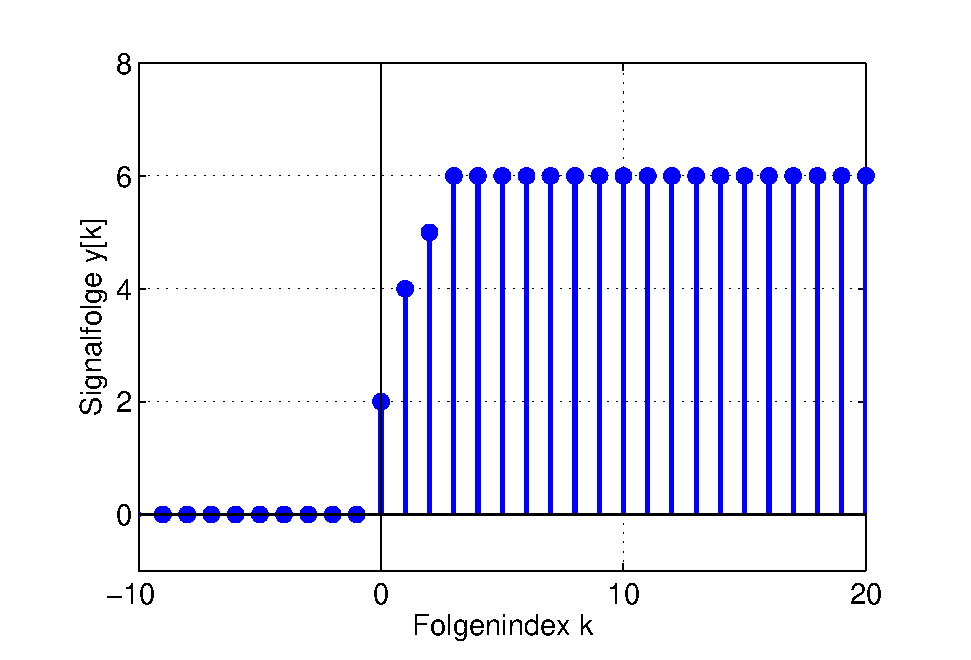
\includegraphics[width=0.5\textwidth]{Kapitel2/Bilder/image16}}
  \caption{Sprungantwort h(t) und Impulsantwort g(t) als Ausgangssignal eines energiefreien LTI-Systems}
  \label{fig:EnergiefreiLTI}
\end{figure}

\noindent F\"{u}r das Beispiel des RC-Netzwerks ergibt sich die Antwort auf einen Sprung der H\"{o}he U${}_{E0}$ = 1 mit der Bedingung u${}_{A}$(0) = 0 zu 

\begin{equation}\label{eq:threehundredfourtyeight}
h\left(t\right)={\rm \; }\left(1-e^{-\frac{t}{R\cdot C} } \right)\cdot \sigma \left(t\right)
\end{equation}

\noindent Wie bereits in Bild \ref{fig:EnergiefreiLTI} dargestellt ist die Impulsantwort g(t) eines Systems die Reaktion eines energiefreien Systems auf eine Anregung mit einem Impuls $\delta$(t). Im Kapitel Signale wird gezeigt, dass die Impulsfunktion $\delta$(t) als Ableitung der Sprungfunktion $\sigma$(t) gedeutet werden kann. 

\begin{equation}\label{eq:threehundredfourtynine}
\delta \left(t\right)=\frac{d\sigma }{dt}
\end{equation}

\noindent F\"{u}r lineare, zeitinvariante Systeme ergibt sich die Systemreaktion auf einen Impuls am Eingang aus der Ableitung der Sprungantwort.

\begin{equation}\label{eq:threehundredfifty}
g\left(t\right)=\frac{dh}{dt} 
\end{equation}

\noindent Bei bekannter Sprungantwort h(t) kann mit Gleichung \eqref{eq:threehundredfifty} die Impulsantwort g(t) durch Ableiten bestimmt werden. Zum Beispiel ergibt sich die Systemantwort eines RC-Netzwerks auf einen Impuls mit dem Gewicht U${}_{E0}$ = 1 mit der Produktregel zu

\begin{equation}\label{eq:threehundredfiftyone}
\begin{split}
g\left(t\right) & = \frac{dh}{dt} =\frac{d}{dt} {\rm \; }\left(\left(1-e^{-\frac{t}{R\cdot C} } \right)\cdot \sigma \left(t\right)\right)=\frac{1}{R\cdot C} \cdot e^{-\frac{t}{R\cdot C} } \cdot U_{E0} \cdot \sigma \left(t\right)-\left(1-e^{-\frac{t}{R\cdot C} } \right)\cdot \delta \left(t\right) \\ 
& = {\frac{1}{R\cdot C} \cdot e^{-\frac{t}{R\cdot C} } \cdot U_{E0} \cdot \sigma \left(t\right)}    
\end{split}
\end{equation}

\subsubsection{Berechnung der Systemantwort durch Superposition}\label{threethreefive}

\noindent Aufgrund der Linearität eines LTI-Systems kann die Systemantwort auf ein aus grundlegenden Funktionen zusammengesetztes Eingangssignal durch die entsprechende Kombination der Ausgangssignale bestimmt werden. Wird zum Beispiel das RC-Netzwerk aus Bild \ref{fig:RCSchaltbild} mit einer Rechteckfunktion der Länge t${}_{0}$ und der Höhe U${}_{E0}$ beaufschlagt, kann das Eingangssignal als Summe zweier Sprungfunktionen dargestellt werden

\begin{equation}\label{eq:threehundredfiftytwo}
u_{E} \left(t\right)=U_{E0} \cdot \left(\sigma \left(t\right)-\sigma \left(t-t_{0} \right)\right)=U_{E0} \cdot \sigma \left(t\right)-U_{E0} \cdot \sigma \left(t-t_{0} \right)
\end{equation}

\noindent Damit ergibt sich das Ausgangsignal u${}_{A}$ aus der Summe der beiden Sprungantworten

\begin{equation}\label{eq:threehundredfiftythree}
u_{A} \left(t\right)=U_{E0} \cdot \left(h\left(t\right)-h\left(t-t_{0} \right)\right)=U_{E0} \cdot \left(1-e^{-\frac{t}{R\cdot C} } \right)\cdot \sigma \left(t\right)-U_{E0} \cdot \left(1-e^{-\frac{t-t_{0} }{R\cdot C} } \right)\cdot \sigma \left(t-t_{0} \right)
\end{equation}

\noindent Bild \ref{fig:RCEinschwingenRechteck} stellt das Superpositionsprinzip für das Beispiel des RC-Netzwerks bei Anregung mit einem rechteckförmigen Signal dar.

\begin{figure}[H]
  \centerline{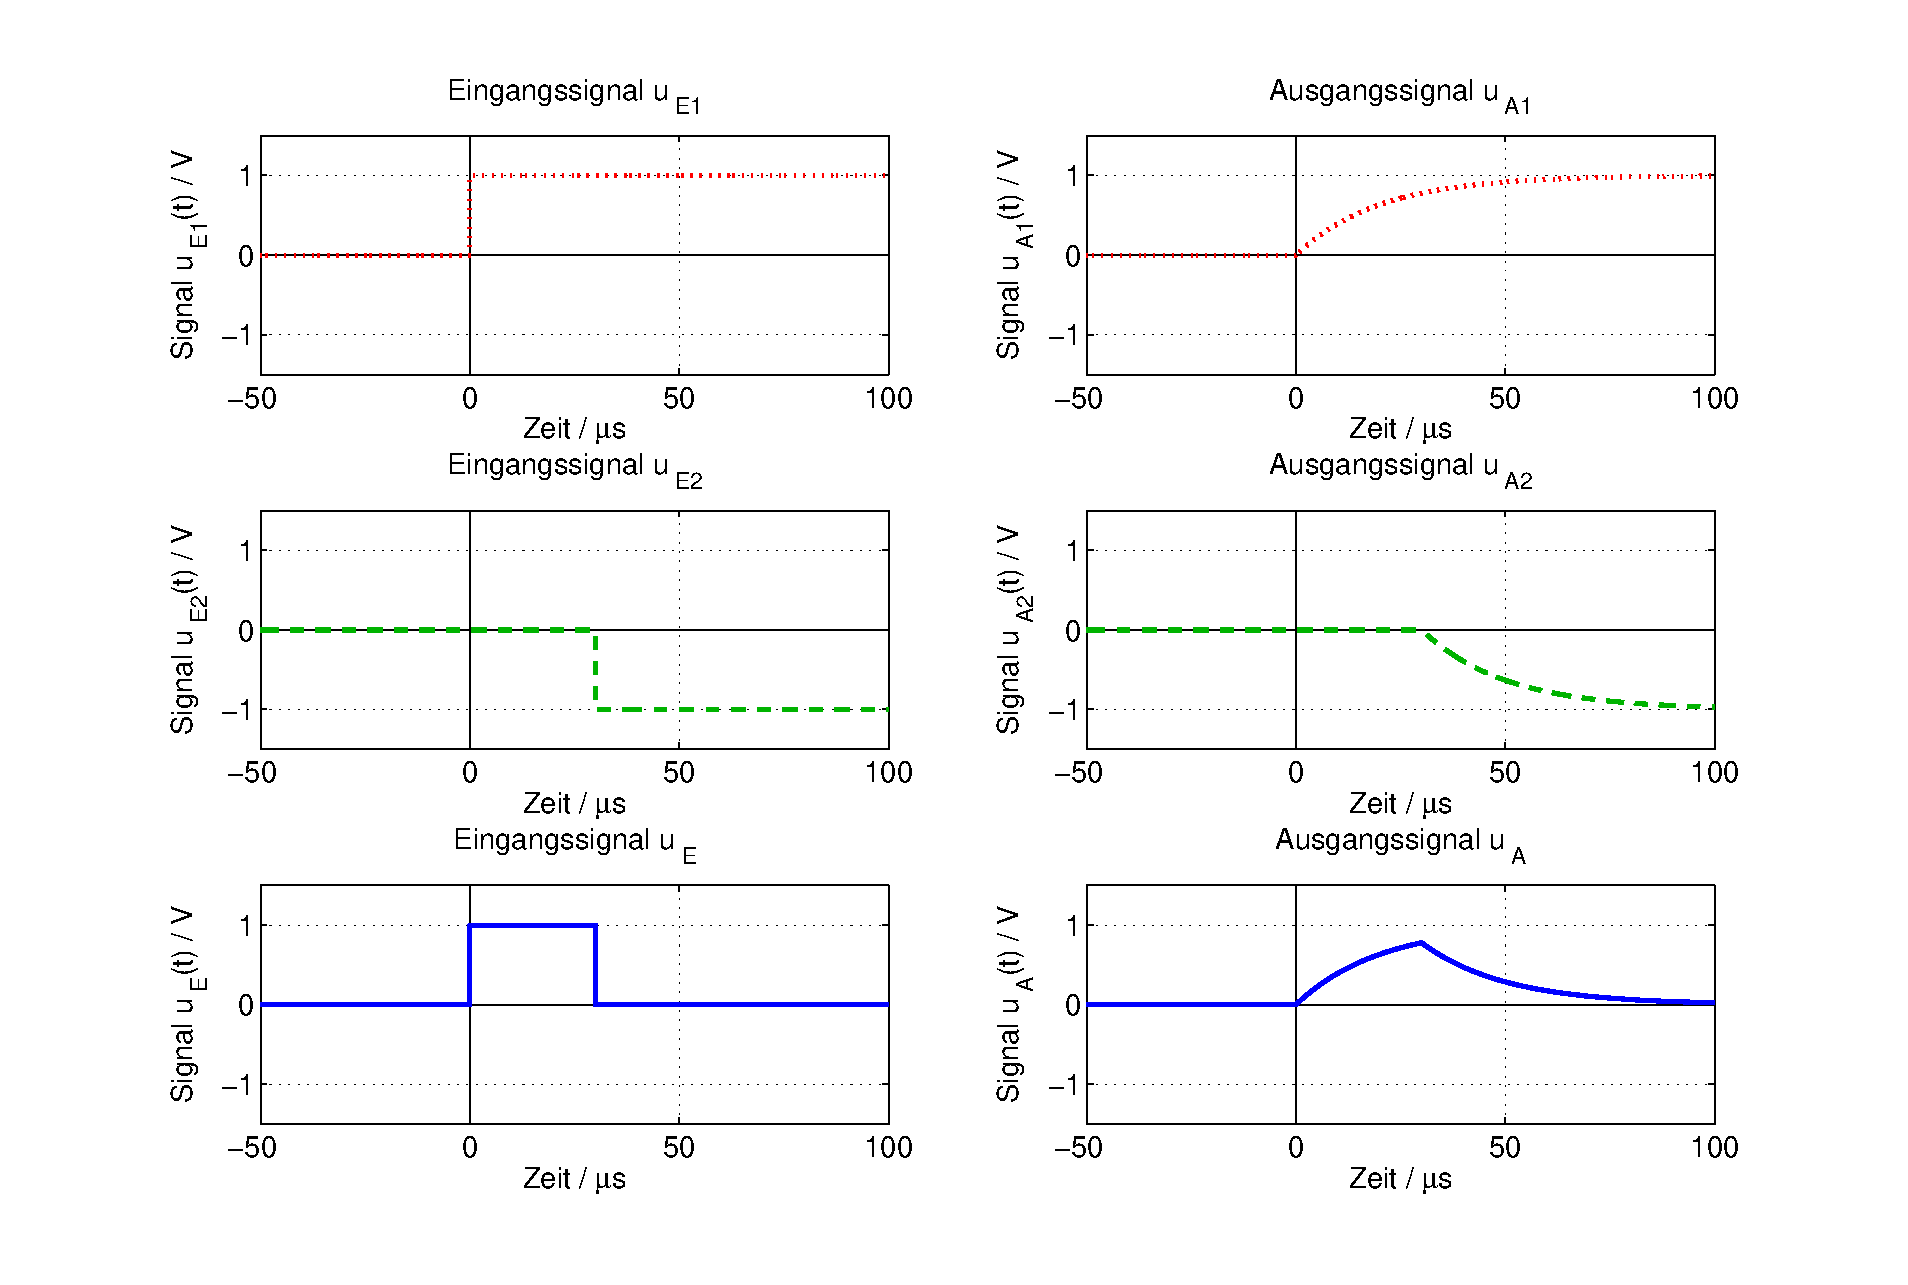
\includegraphics[width=1\textwidth]{Kapitel2/Bilder/image17}}
  \caption{Überlagerung der Systemreaktion u${}_{A}$ = u${}_{A1}$+ u${}_{A2}$ bei überlagertem Eingangssignal u${}_{E}$ = u${}_{E}$ + u${}_{E2}$}
  \label{fig:RCEinschwingenRechteck}
\end{figure}

\noindent Mit der Kenntnis der Sprungantwort eines Systems kann demnach für grundlegende Eingangs-signale, die sich über die Sprungfunktion darstellen lassen, eine Systemantwort berechnet werden. 

\subsection{Berechnung der Systemantwort über das Faltungsintegral}

\noindent In dem vorangegangenen Abschnitt werden mit der Linearitätseigenschaft und Zeitinvarianz eines Systems sowie der Sprungantwort h(t) Systemantworten auf andere Eingangssignale bestimmt. Die Näherung einer beliebigen Eingangsfunktion durch eine große Anzahl kleiner Impulse führt zur Bestimmung der Systemantwort über das Faltungsintegral, das im Folgenden hergeleitet wird. 

\subsubsection{Herleitung des Faltungsintegrals}

\noindent Ein lineares, zeitinvariantes System antwortet auf einen Impuls $\delta$(t) am Eingang mit der Impulsantwort g(t). Entsprechend antwortet es auf eine Linearkombination von Impulsen

\begin{equation}\label{eq:threehundredfiftyfour}
u\left(t\right)=\nu _{1} \cdot \delta \left(t\right)+\nu _{2} \cdot \delta \left(t-3\right)
\end{equation}

\noindent mit der gleichen Linearkombination von Impulsantworten

\begin{equation}\label{eq:threehundredfiftyfive}
y\left(t\right)=\nu _{1} \cdot g\left(t\right)+\nu _{2} \cdot g\left(t-3\right)
\end{equation}

\noindent Dieser Zusammenhang kann auf beliebige Eingangssignale verallgemeinert werden. Wegen der Ausblendeigenschaft der Impulsfunktion kann ein beliebiges Eingangssignal u(t) dargestellt werden als 

\begin{equation}\label{eq:threehundredfiftysix}
u\left(t\right)=u\left(t\right)\cdot \int\limits _{-\infty }^{\infty }\delta \left(t-\tau \right)\;d\tau  =\int\limits _{-\infty }^{\infty }u\left(t\right)\cdot \delta \left(t-\tau \right)\;d\tau  =\int\limits _{-\infty }^{\infty }u\left(\tau \right)\cdot \delta \left(t-\tau \right)\;d\tau 
\end{equation}

\noindent Anschaulich kann die Gleichung als Superposition unendlich vieler Impulse $\delta$(t - $\tau$) mit dem Gewicht u($\tau$) interpretiert werden, die zusammen das Signal u(t) darstellen. Jeder einzelne Impuls $\delta$(t - $\tau$) besitzt die Systemantwort g(t - $\tau$). Damit ergibt sich das Ausgangssignal y(t) aus der Superposition unendlich vieler Systemantworten g(t - $\tau$) mit dem Gewicht u($\tau$).

\begin{equation}\label{eq:threehundredfiftyseven}
y\left(t\right)=\int _{-\infty }^{\infty }u\left(\tau \right)\cdot g\left(t-\tau \right){\rm \; }d\tau  =u\left(t\right)*g\left(t\right)
\end{equation}

\noindent Bei bekannter Impulsantwort g(t) kann das Ausgangssignal y(t) für eine beliebige Systemanregung u(t) aus der Integralgleichung \eqref{eq:threehundredfiftyseven} berechnet werden. Das Integral wird als Faltungsintegral bezeichnet. Abkürzend wird die Faltungsoperation mit einem $*$ - Symbol dargestellt.

\subsubsection{Grafische Interpretation des Faltungsintegrals}

\noindent Das Faltungsintegral erscheint zunächst kompliziert und wenig griffig. Es kann aber grafisch interpretiert werden. Dazu wird das Faltungsintegral umgeformt zu

\begin{equation}\label{eq:threehundredfiftyeight}
y\left(t\right)=\int\limits _{-\infty }^{\infty }u\left(\tau \right)\cdot g\left(t-\tau \right)\;d\tau  =\int\limits _{-\infty }^{\infty }u\left(\tau \right)\cdot g\left(-\left(\tau -t\right)\right)\;d\tau 
\end{equation}

\noindent Das Faltungsintegral wird für einen festen Zeitpunkt t ausgewertet. Es ist die Fläche unter einer Funktion, die sich aus dem Produkt zweier Teilfunktionen ergibt. Eine Teilfunktion ist das bekannte Eingangssignal u($\tau$). Die zweite Teilfunktion ist die berechnete Impulsantwort g($\tau$), die jedoch an der Achse $\tau$ = 0 gespiegelt und um t nach rechts verschoben ist. \medskip

\noindent Aus dieser Interpretation ergibt sich folgendes Vorgehen zur grafischen Auswertung des Faltungsintegrals:

\begin{itemize}
\item  Skizzieren der Funktion u($\tau$)

\item  Skizzieren der Funktion g(-($\tau$ - t)) durch Spiegeln der Funktion g($\tau$) und Verschiebung um t nach rechts

\item  Berechnen des Produktes der beiden Funktionen u($\tau$)$.$g(-($\tau$ - t))

\item  Auswertung der Fl\"{a}che unter der Kurve u($\tau$)$.$g(-($\tau$ - t))
\end{itemize}

\noindent Das Verständnis der grafischen Faltung ist Grundlage für die Berechnung von Ausgangssignalen im Zeitbereich mit dem Faltungsintegral.\bigskip

\noindent
\colorbox{lightgray}{%
\arrayrulecolor{white}%
\renewcommand\arraystretch{0.6}%
\begin{tabular}{ wl{16.5cm} }
{\fontfamily{phv}\selectfont{
Beispiel: Grafische Faltung zweier Rechteckfunktionen}}
\end{tabular}%
}\bigskip

\noindent Das Vorgehen wird an der Faltung zweier Rechteckfunktionen verdeutlicht. 

\begin{equation}\label{eq:threehundredfiftynine}
u\left(t\right)=\sigma \left(t\right)-\sigma \left(t-2\right)
\end{equation}

\begin{equation}\label{eq:threehundredsixty}
g\left(t\right)=2\cdot \left(\sigma \left(t\right)-\sigma \left(t-4\right)\right)
\end{equation}

\noindent Zur grafischen Auswertung des Integrals werden beide Funktionen als Funktion der Variablen $\tau$ dargestellt, nach der integriert werden soll. 

\begin{equation}\label{eq:threehundredsixtyone}
u\left(\tau \right)=\sigma \left(\tau \right)-\sigma \left(\tau -2\right)
\end{equation}

\begin{equation}\label{eq:threehundredsixtytwo}
g\left(\tau \right)=2\cdot \left(\sigma \left(\tau \right)-\sigma \left(\tau -4\right)\right)
\end{equation}

\noindent Die Funktion g wird an der Achse $\tau$ = 0 gespiegelt 

\begin{equation}\label{eq:threehundredsixtythree}
g\left(-\tau \right)=2\cdot \left(\sigma \left(-\tau \right)-\sigma \left(-\left(\tau -4\right)\right)\right)
\end{equation}

\noindent und anschlie{\ss}end um t nach rechts verschoben. 

\begin{equation}\label{eq:threehundredsixtyfour}
g\left(t-\tau \right)=g\left(-\left(\tau -t\right)\right)=2\cdot \left(\sigma \left(-\left(\tau -t\right)\right)-\sigma \left(-\left(\tau -t-4\right)\right)\right)
\end{equation}

\noindent Bild \ref{fig:FaltungGrafischRechtecke} stellt die Funktionen f\"{u}r unterschiedliche Zeitpunkte t dar. Das Integral der Faltungsfunktion berechnet sich aus der Fl\"{a}che, die unter dem Produkt der beiden Funktionen u($\tau$) und g(t - $\tau$) liegt. F\"{u}r t = 0 \"{u}berschneiden sich die Funktionsbereiche, die ungleich null sind, nicht. Das Produkt der beiden Funktionen ist f\"{u}r t = 0 null. F\"{u}r negative Werte von t ist das ebenfalls der Fall, wie an dem Beispiel f\"{u}r t = - 1 deutlich wird. F\"{u}r positive Werte von t \"{u}berschneiden sich die Funktionsbereiche, in den die Funktionen ungleich null sind. Das gilt f\"{u}r den Bereich 0 $\leq$ t $\mathrm{<}$ 6. F\"{u}r den Bereich 2 $\leq$ t $\mathrm{<}$ 4 \"{u}berdecken sich die Funktionen komplett, hier ergibt sich ein konstanter Wert des Faltungsintegrals von 4, da die Fl\"{a}che in diesem Bereich konstant bleibt. F\"{u}r t $\mathrm{>}$ 6 liegt wieder keine \"{U}berschneidung vor, das Produkt der Funktionen ist f\"{u}r alle $\tau$ null.

\begin{figure}[H]
  \centerline{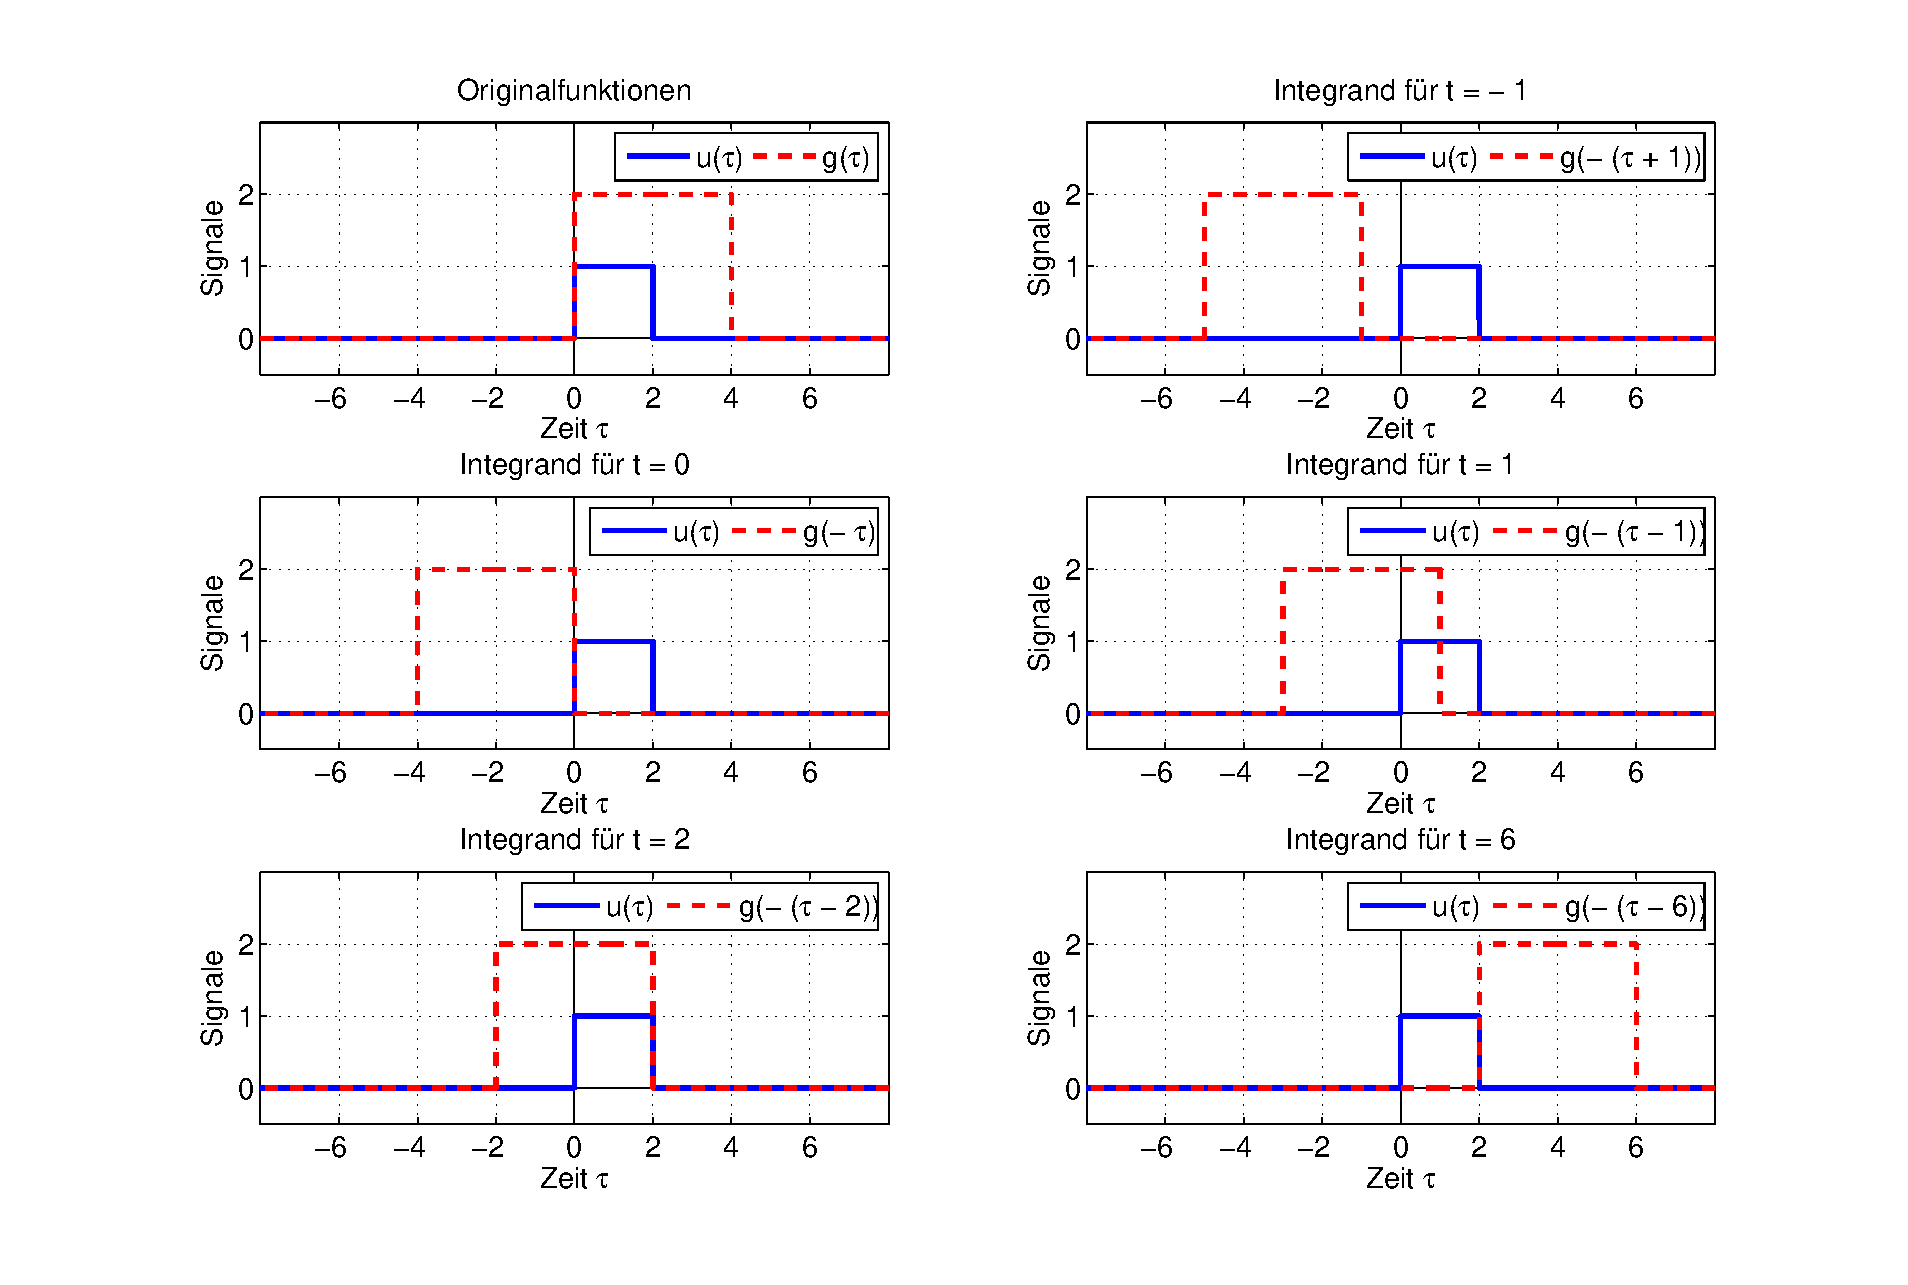
\includegraphics[width=1\textwidth]{Kapitel2/Bilder/image18}}
  \caption{Darstellung der Schritte zur grafischen Faltung am Beispiel zweier Rechtecke}
  \label{fig:FaltungGrafischRechtecke}
\end{figure}

\noindent Für einen festen Zeitpunkt t ergibt sich der Wert des Faltungsintegrals aus der Fläche unter der Rechteckfunktion. Durch Verschiebung der Funktion g ändert sich die Fläche, und es ergibt sich der in 
Bild \ref{fig:FaltungGrafischRechteckeBSP} dargestellte Verlauf des Faltungsintegrals.

\begin{figure}[H]
  \centerline{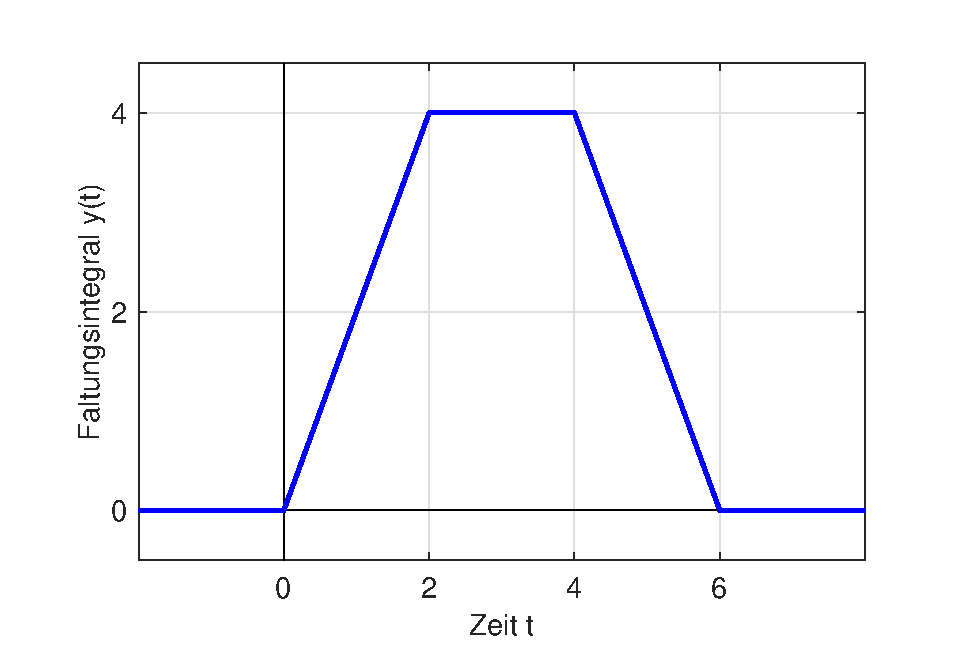
\includegraphics[width=0.5\textwidth]{Kapitel2/Bilder/image19}}
  \caption{Darstellung des Faltungsintegrals für das Beispiel zweier Rechtecke}
  \label{fig:FaltungGrafischRechteckeBSP}
\end{figure}

\noindent
\noindent

\InsertBoxL{0}{\includegraphics[scale=0.5]{code}} 
\textcolor{white}{.}\newline
\noindent Im Online-Portal \textit{Systemtheorie Online} verdeutlicht die Applikation \textit{Komplexe Exponentialfunktion} den Zusammenhang zwischen der Lage des Wertes $\lambda = \delta + j.\omega{}_{0}$ in der komplexen Ebene und dem Verhalten der Schwingung.\newline

\subsubsection{Rechenregeln zum Faltungsintegral}

\noindent Zur Berechnung des Faltungsintegrals existieren verschiedene Rechenregeln, die im Folgenden zusammengefasst werden. Die Herleitungen beruhen auf den Rechenregeln für Integrale und sind zum Beispiel in [Foel11] zu finden. Hier werden das Kommutativgesetz sowie die Rechen-regeln zur Faltung mit einem Impuls und die Faltung zweier kausaler Signale hergeleitet.\bigskip

\noindent\textbf{\fontfamily{phv}\selectfont{{Kommutativgesetz der Faltung}}}

\noindent In einigen Fällen ergeben sich Rechenvorteile, wenn das Kommutativgesetz der Faltung genutzt werden kann. Die Herleitung beginnt mit der Definitionsgleichung des Faltungsintegrals.

\begin{equation}\label{eq:threehundredsixtyfive}
y\left(t\right)=\int\limits _{-\infty }^{\infty }u\left(\tau \right)\cdot g\left(t-\tau \right)\;d\tau
\end{equation}

\noindent Mit der Substitution

\begin{equation}\label{eq:threehundredsixtysix}
\tau =t-x
\end{equation}

\noindent und der Ableitung

\begin{equation}\label{eq:threehundredsixtyseven}
\frac{d\tau }{dx} =-1
\end{equation}

\noindent ergibt sich 

\begin{equation}\label{eq:threehundredsixtyeight}
\begin{split}
y\left(t\right) & = \int\limits _{-\infty }^{\infty }u\left(\tau \right)\cdot g\left(t-\tau \right)\;d\tau  =-\int\limits _{\infty }^{-\infty }u\left(t-x\right)\cdot g\left(x\right)\;dx =\int\limits _{-\infty }^{\infty }u\left(t-x\right)\cdot g\left(x\right)\;dx \\
& = \int\limits _{-\infty }^{\infty } u\left(t-\tau\right)\cdot g(\tau) \; d\tau
\end{split}
\end{equation}

\noindent Das Ergebnis ist wieder ein Faltungsintegral. Allerdings wird bei diesem Faltungsintegral die Funktion u(t) an der Achse $\tau$ = 0 gespiegelt und um t verschoben. Es gilt das Kommutativgesetz.

\begin{equation}\label{eq:threehundredsixtynine}
u\left(t\right)*g\left(t\right)=g\left(t\right)*u\left(t\right)
\end{equation}

\noindent Der Integrand ist an allen Stellen null, nur nicht an der Stelle $\tau$ = t$_{0}$. Damit kann das Integral umgeformt werden zu

\begin{equation}\label{eq:threehundredseventy}
u\left(t\right)*\delta \left(t-t_{0} \right)=\int\limits _{-\infty }^{\infty }u\left(t-\tau \right)\cdot \delta \left(\tau -t_{0} \right)\;d\tau
\end{equation}

\noindent Der Integrand ist an allen Stellen null, nur nicht an der Stelle $\tau$ = t${}_{0}$. Damit kann das Integral umgeformt werden zu

\begin{equation}\label{eq:threehundredseventyone}
\int\limits _{-\infty }^{\infty }u\left(t-\tau \right)\cdot \delta \left(\tau -t_{0} \right){\rm \; }d\tau  =u\left(t-t_{0} \right)\cdot \int\limits _{-\infty }^{\infty }\delta \left(\tau -t_{0} \right){\rm \; }d\tau 
\end{equation}

\noindent Da das Integral \"{u}ber eine Impulsfunktion immer eins ist, ergibt sich

\begin{equation}\label{eq:threehundredseventytwo}
u\left(t\right)*\delta \left(t-t_{0} \right)=u\left(t-t_{0} \right)\cdot \int\limits _{-\infty }^{\infty }\delta \left(\tau -t_{0} \right)\;d\tau  =u\left(t-t_{0} \right)
\end{equation}

\noindent Die Faltung eines Signals u(t) mit einem Impuls an der Stelle t${}_{0}$ verschiebt das Signal an die Stelle des Impulses. \bigskip

\noindent
\colorbox{lightgray}{%
\arrayrulecolor{white}%
\renewcommand\arraystretch{0.6}%
\begin{tabular}{ wl{16.5cm} }
{\fontfamily{phv}\selectfont
\noindent
Beispiel: Grafische Faltung eines Signals mit einem Impuls}
\end{tabular}%
}\bigskip

\noindent Bild \ref{fig:FaltungGrafischImpuls} stellt die Faltung eines Signals mit einem um t${}_{0}$ = 6 verschobenen Impuls dar. Das Ergebnis kann so hergeleitet werden, dass der Impuls $\deltaup$(t - 6 - $\tau$) an dem Signal u(t) vorbei geschoben wird. Das Produkt der beiden Signale ist nur in dem Bereich 4 $\leq$ t $\mathrm{<}$ 8 ungleich null, in den anderen Bereichen ist mindestens eine der beiden Funktionen null.

\begin{figure}[H]
  \centerline{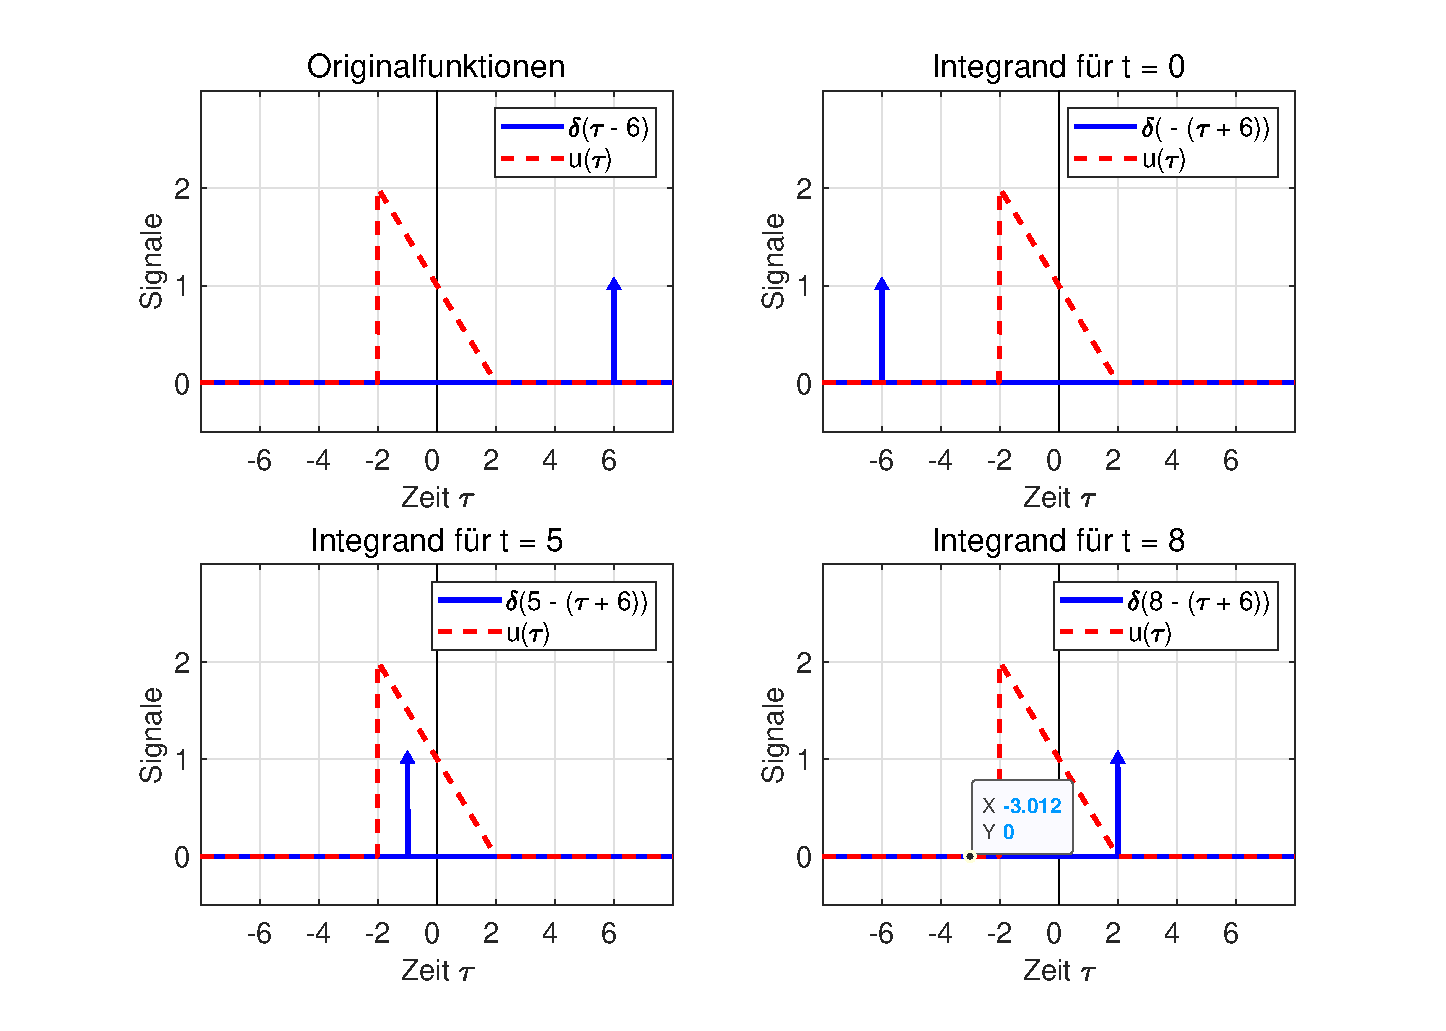
\includegraphics[width=1\textwidth]{Kapitel2/Bilder/image20}}
  \caption{Grafische Faltung eines Signals u(t) mit einem Impuls an der Stelle t$_{0}$ = 6}
  \label{fig:FaltungGrafischImpuls}
\end{figure}

\noindent Die Auswertung der grafischen Faltung ist in Bild \ref{fig:FaltungGrafischImpulsBSP} dargestellt. Die Funktion u(t) ist um t$_{0}$ nach rechts verschoben worden.

\begin{figure}[H]
  \centerline{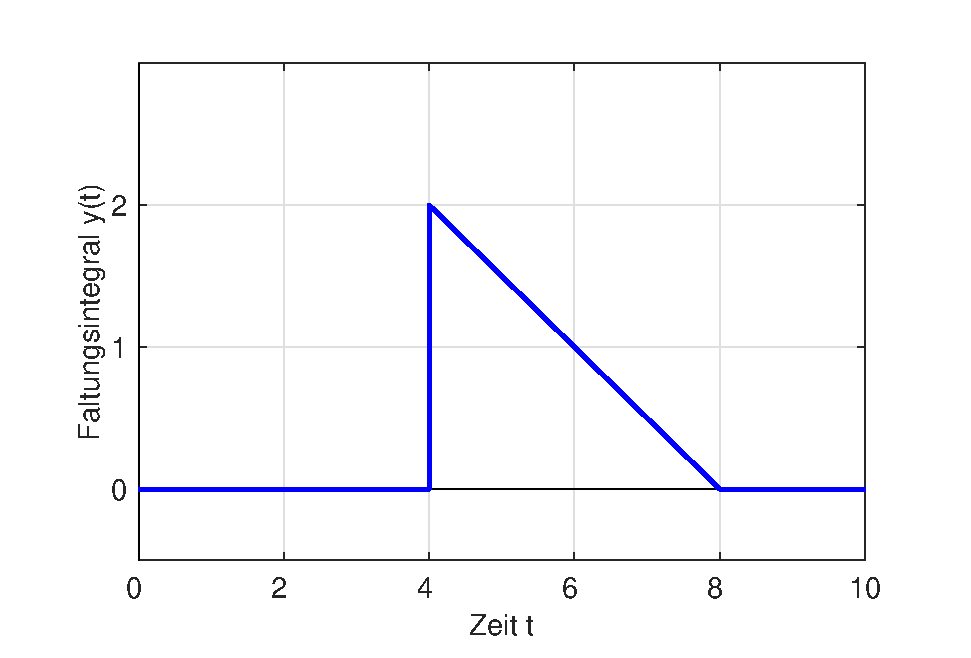
\includegraphics[width=0.5\textwidth]{Kapitel2/Bilder/image21}}
  \caption{Ergebnis der grafischen Faltung eines Signals u(t) mit einem Impuls an der Stelle t$_{0}$ = 6}
  \label{fig:FaltungGrafischImpulsBSP}
\end{figure}

\clearpage

{\fontfamily{phv}\selectfont
\noindent\textbf{Faltung kausaler Funktionen}}\smallskip

\noindent Sind die Funktionen g(t) und u(t) kausale Funktionen, reduziert sich das Faltungsintegral auf den Bereich von 0 … t. Dieses Ergebnis ergibt sich unmittelbar aus der grafischen Faltung. 

\begin{figure}[H]
  \centerline{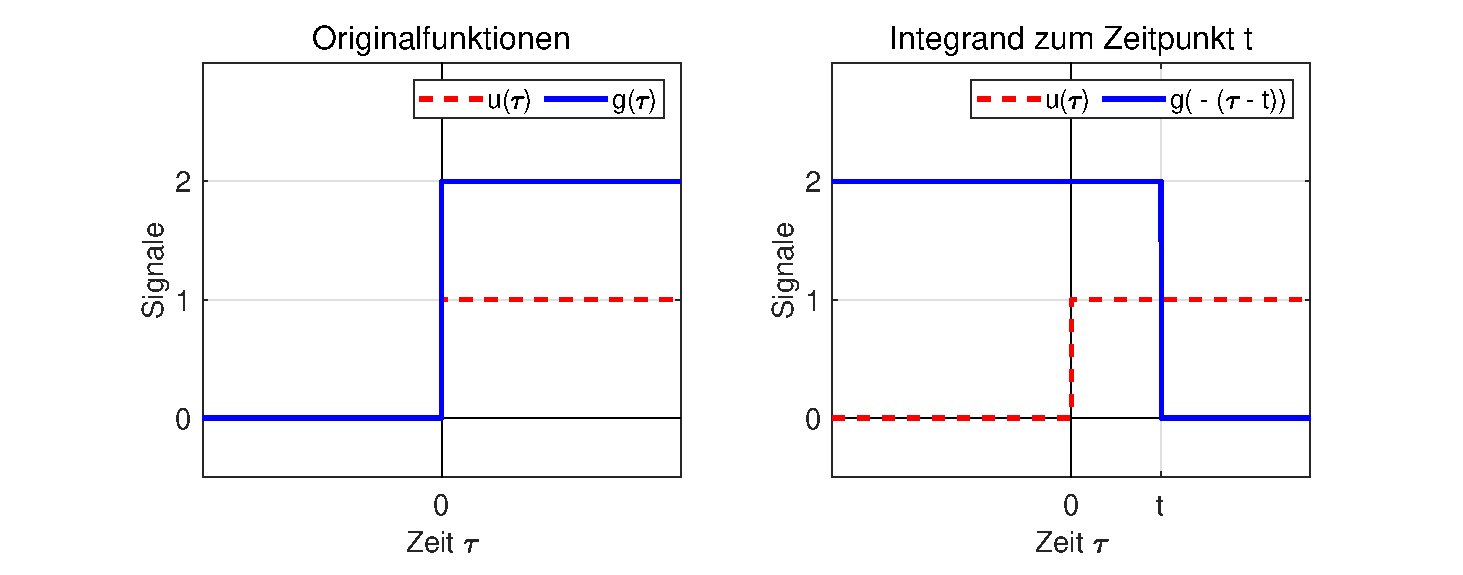
\includegraphics[width=1\textwidth]{Kapitel2/Bilder/image22}}
  \caption{Faltung kausaler Funktionen}
  \label{fig:FaltungKausal}
\end{figure}

\noindent Die Funktion u($\tau$) ist f\"{u}r den Bereich $\tau$ $\mathrm{<}$ 0 null, die Funktion g(t - $\tau$) ist f\"{u}r den Bereich $\tau$ $\mathrm{>}$ t null. Damit ist das Produkt der beiden Funktionen nur in dem Bereich von 0 {\dots} t von null verschieden. F\"{u}r kausale Funktionen gilt deshalb

\begin{equation}\label{eq:threehundredseventythree}
y\left(t\right)=\int _{-\infty }^{\infty }u\left(\tau \right)\cdot g\left(t-\tau \right){\rm \; }d\tau  =\int _{0}^{t}u\left(\tau \right)\cdot g\left(t-\tau \right){\rm \; }d\tau 
\end{equation}

\clearpage

{\fontfamily{phv}\selectfont
\noindent\textbf{Zusammenfassung der Rechenregeln zum Faltungsintegral}}

\noindent Die wesentlichen Rechenregeln für das Faltungsintegral sind in Tabelle 3.8 zusammengefasst.

\begin{table}[H]
\caption{Zusammenhang zwischen Lösungen der charakteristischen Gleichung und der Stabilität von LTI-Systemen, die sich über lineare Differentialgleichungen mit konstanten Koeffizienten beschreiben lassen }
\setlength{\fboxsep}{0pt}%
\colorbox{lightgray}{%
\arrayrulecolor{white}%
\begin{tabular}{| c | c |}
\hline
\parbox[c][0.28in][c]{3.3in}{\smallskip\centering\textbf{\fontfamily{phv}\selectfont{Gesetz}}} & \parbox[c][0.28in][c]{3.3in}{\smallskip\centering\textbf{\fontfamily{phv}\selectfont{Mathematische Beschreibung}}}\\ \hline

\parbox[c][0.7in][c]{3.3in}{\centering{\fontfamily{phv}\selectfont{Kommutativgesetz}}} &
\parbox[c][0.7in][c]{3.3in}{\centering{
$u\left(t\right)*g\left(t\right)=g\left(t\right)*u\left(t\right)$
}}\\ \hline

\parbox[c][0.8in][c]{3.3in}{\centering{\fontfamily{phv}\selectfont{Assoziativgesetz}}} & 
\parbox[c][0.8in][c]{3.3in}{\centering{
$\left(x\left(t\right)*u\left(t\right)\right)*g\left(t\right)=x\left(t\right)*\left(u\left(t\right)*g\left(t\right)\right)$
}}\\ \hline

\parbox[c][0.8in][c]{3.3in}{\centering{\fontfamily{phv}\selectfont{Distributivgesetz}}} &
\parbox[c][0.8in][c]{3.3in}{\centering{
$\left(u_{1} \left(t\right)+u_{2} \left(t\right)\right)*g\left(t\right)=u_{1} \left(t\right)*g\left(t\right)+u_{2} \left(t\right)*g\left(t\right)$
}}\\ \hline

\parbox[c][0.8in][c]{3.3in}{\centering{\fontfamily{phv}\selectfont{Faltung kausaler Signale}}} &
\parbox[c][0.8in][c]{3.3in}{\centering{
$\int _{-\infty }^{\infty }u\left(\tau \right)\cdot g\left(t-\tau \right){\rm \; }d\tau  =\int _{0}^{t}u\left(\tau \right)\cdot g\left(t-\tau \right){\rm \; }d\tau  $ 
}}\\ \hline

\parbox[c][0.8in][c]{3.3in}{\centering{\fontfamily{phv}\selectfont{Faltung mit einem Impuls an der Stelle $t_{0}$}}} &
\parbox[c][0.8in][c]{3.3in}{\centering{
$u\left(t\right)*\delta \left(t-t_{0} \right)=u\left(t-t_{0} \right)$
}}\\ \hline

\end{tabular}%
}\bigskip
\label{tab:threeeight}
\end{table}

\subsubsection{Anwendung des Faltungsintegrals am Beispiel des RC-Netzwerks}\label{threefourfour}

\noindent Die Berechnung des Faltungsintegrals wird an einem RC-Netzwerk vertieft, das mit einem recht-eckförmigen Signal angeregt wird. Das Ergebnis wird anschließend mit dem Ergebnis verglichen, das sich bei Anwendung des Superpositionsprinzips ergeben hat. Die Impulsantwort g(t) des RC-Netzwerks lautet

\begin{equation}\label{eq:threehundredseventyfour}
g\left(t\right)=\frac{1}{R\cdot C} \cdot e^{-\frac{t}{R\cdot C} } \cdot \sigma \left(t\right)
\end{equation}

\noindent Das Eingangssignal ist definiert als

\begin{equation}\label{eq:threehundredseventyfive}
u_{E} \left(t\right)=\left\{\begin{array}{l} 
{U_{{\rm E0}} \qquad  \text{ für } \; 0\le  t<\rm t_{0} } \\ 
0\qquad \quad \;\, \text{sonst}
\end{array}\right.
\end{equation}

\noindent Beide Signale sind kausal, sodass sich das Ausgangssignal u${}_{A}$(t) ergibt

\begin{equation}\label{eq:threehundredseventysix}
u_{A} \left(t\right)=\int _{0}^{t}u_{E} \left(\tau \right)\cdot g\left(t-\tau \right)\;d\tau
\end{equation}

\noindent Zur Auswertung des Integrals muss analysiert werden, wann sich die beiden Funktionen g(t - $\tau$) und u${}_{E}$($\tau$) \"{u}berlappen. Dazu zeigt Bild \ref{fig:FaltungGrafischRCNetzwerk} die Funktionen g(t - $\tau$) und u${}_{E}$($\tau$) f\"{u}r unterschiedliche Zeitpunkte t.

\begin{figure}[H]
  \centerline{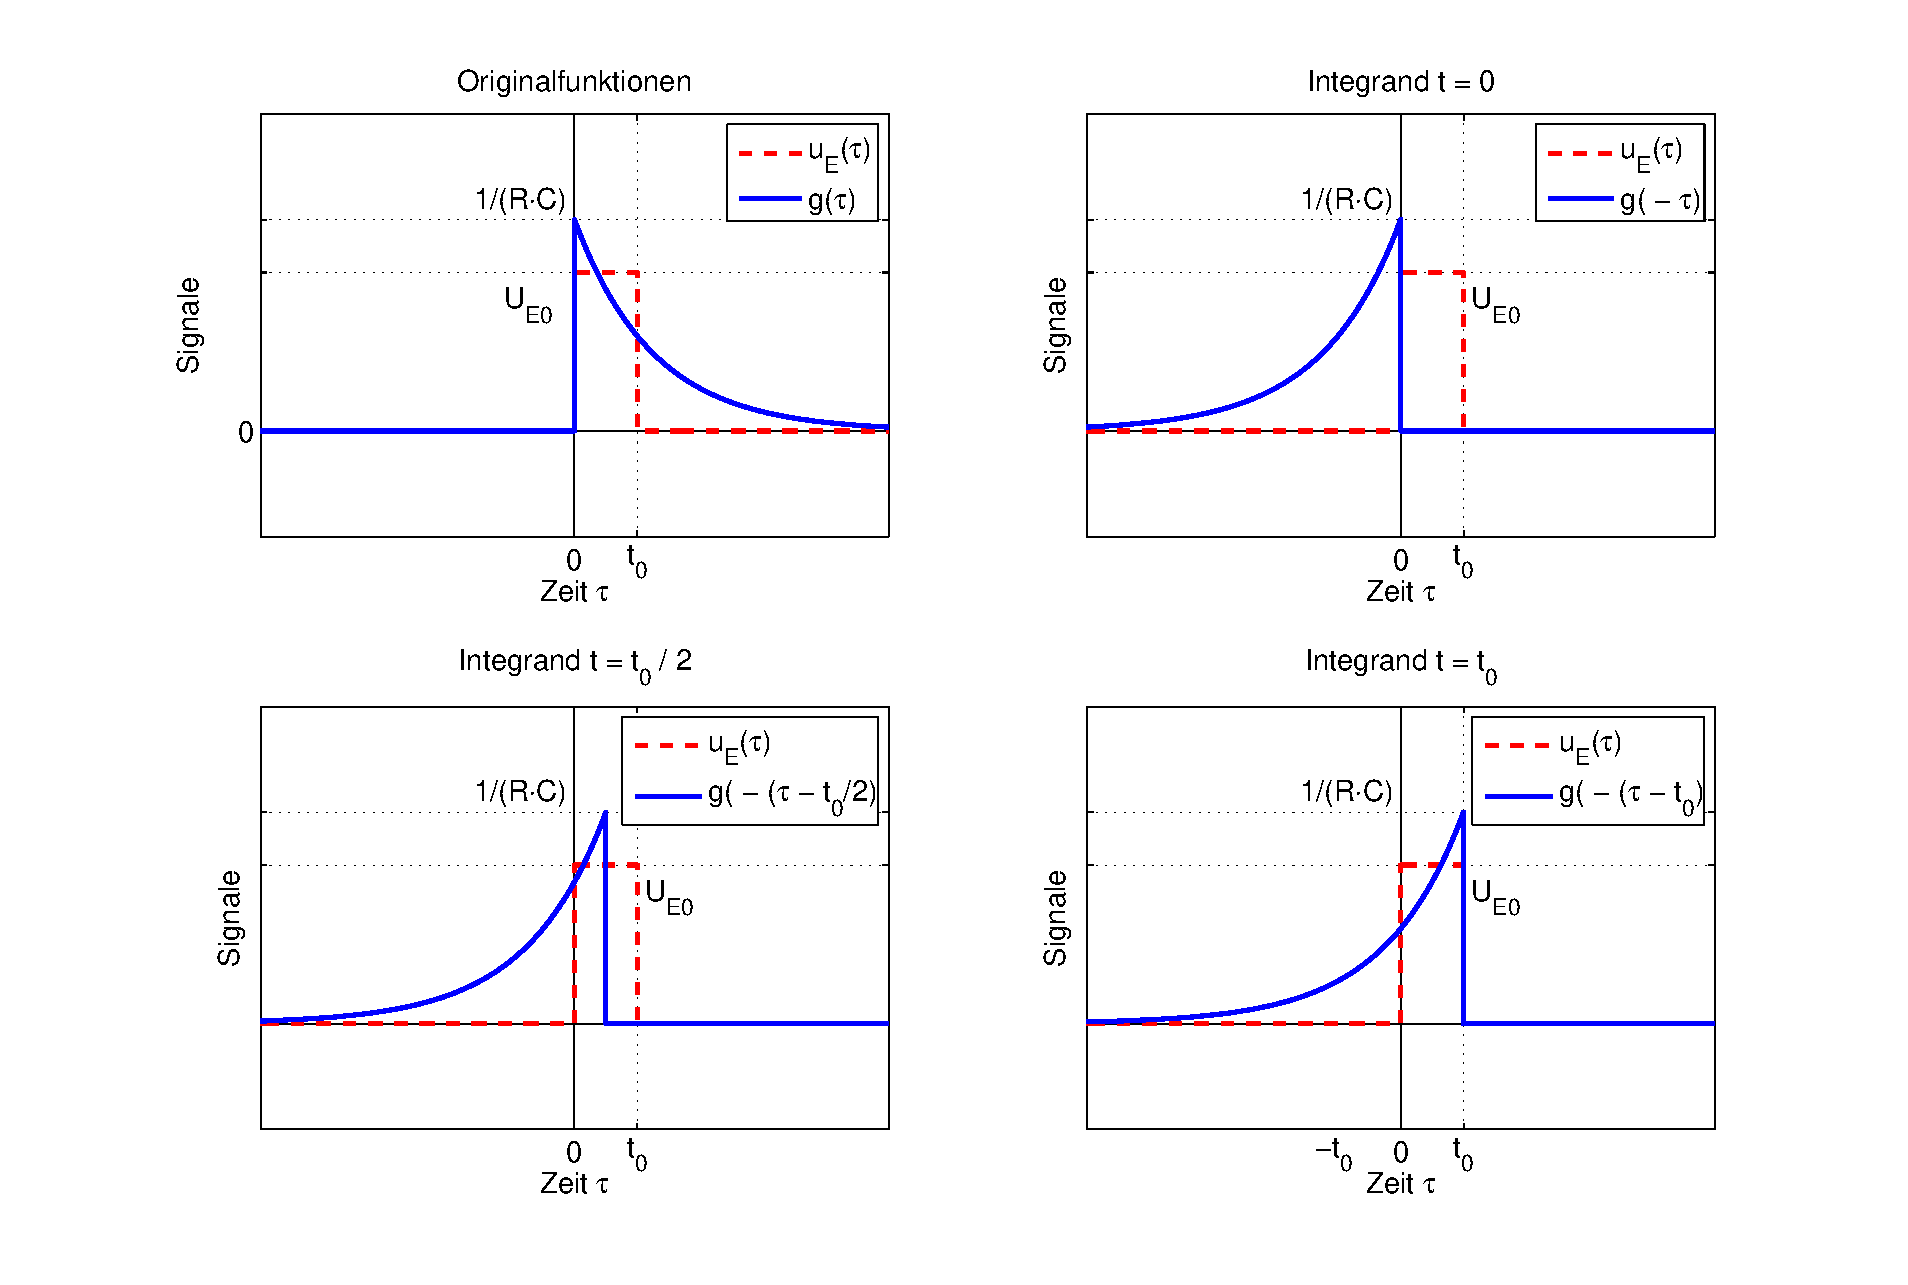
\includegraphics[width=1\textwidth]{Kapitel2/Bilder/image23}}
  \caption{Darstellung der Funktionen g(t - $\tau$) und u${}_{E}$($\tau$) zur Berechnung des Faltungsintegrals f\"{u}r verschiedene Zeitpunkte t}
  \label{fig:FaltungGrafischRCNetzwerk}
\end{figure}\bigskip

{\fontfamily{phv}\selectfont
\noindent\textbf{Zeitraum  t $\mathrm{<}$ 0}}\smallskip

\noindent F\"{u}r alle $\tau$ ist zumindest eine der beiden Funktionen null, das Faltungsintegral ist damit f\"{u}r t $\mathrm{<}$ 0 null.

\begin{equation}\label{eq:threehundredseventyseven}
u_{A} \left(t\right)=0
\end{equation}\bigskip

{\fontfamily{phv}\selectfont
\noindent\textbf{Zeitraum 0 $\mathrm{<}$ t $\mathrm{<}$ t$_{0}$}}\smallskip

\noindent Die beiden Funktionen \"{u}berlappen sich in dem Bereich 0 $\leq$ $\tau$ $\leq$ t, sodass das Integral in diesem Bereich ausgef\"{u}hrt wird. 

\begin{equation}\label{eq:threehundredseventyeight}
\begin{split}
u_{A} \left(t\right) & = \int\limits _{0}^{t}g\left(t-\tau \right)\cdot U_{E0} \;d\tau  =\int\limits _{0}^{t}U_{E0} \cdot \frac{1}{R\cdot C} \cdot e^{-\frac{t-\tau }{RC} } \;d\tau  =e^{-\frac{t}{RC} } \cdot \int\limits _{0}^{t}U_{E0} \cdot \frac{1}{R\cdot C} \cdot e^{\frac{\tau }{RC} } \;d\tau\\
& =\left. U_{E0}\cdot\frac{1}{R\cdot C}\cdot e^{-\frac{t}{R\cdot C}}\cdot R\cdot C \cdot  e^{\frac{t}{R\cdot C}}\right|_{0}^{t} 
=  U_{E0}\cdot \frac{1}{R\cdot C}\cdot e^{-\frac{t}{R\cdot C}}\cdot R\cdot C (\cdot  e^{\frac{t}{R\cdot C}}-e^{\frac{0}{R\cdot C}})\\
& =  U_{E0} \cdot (1-e^{-\frac{t}{R\cdot C}})
\end{split}
\end{equation}\bigskip
\clearpage

{\fontfamily{phv}\selectfont
\noindent\textbf{Zeitraum t $\geqslant $ t$_{0}$}}\smallskip

\noindent Jetzt überlappen sich die beiden Funktionen ganz und die Integration erstreckt sich von 0 bis t$_{0}$.

\begin{equation}\label{eq:threehundredseventynine}
\begin{split}
u_{A} \left(t\right) & = \int\limits _{0}^{t_{0} }g\left(t-\tau \right)\cdot U_{E0} \;d\tau  =\int\limits _{0}^{t_{0} }U_{E0} \cdot \frac{1}{R\cdot C} \cdot e^{-\frac{t-\tau }{RC} } \; d\tau  =\left. U_{E0} \cdot \frac{1}{R\cdot C} \cdot e^{-\frac{t}{R\cdot C} } \cdot R\cdot C\cdot e^{\frac{\tau }{R\cdot C} } \right|_{0}^{t_{0}} \\ 
& = U_{E0} \cdot e^{-\frac{t}{R\cdot C}} \cdot (e^{\frac{t_{0}}{R\cdot C}}-1) = U_{E0} \cdot (1-e^{-\frac{t_{0}}{R\cdot C}}) \cdot e^{-\frac{t-t_{0}}{R\cdot C}}
\end{split}
\end{equation}

\noindent Damit kann u$_{A}$(t) zusammengefasst werden als

\begin{equation}\label{eq:threehundredeighty}
\begin{split}
u_{A} \left(t\right)=\left\{\begin{array}{l} 
{U_{E0} \cdot \left(1-e^{-\frac{t}{RC} } \right) \qquad \qquad \quad \text{für } 0\leqslant t<t_{0} }\medskip \\ 
{U_{E0} \cdot \left(1-e^{-\frac{t_{0} }{R\cdot C}} \right)\cdot e^{-\frac{t-t_{0} }{R\cdot C}} \qquad \; \text{für } t \ge t_{0\qquad } } \\ 
{} \\ 0 \; \qquad \qquad \qquad \qquad \qquad \quad \text{sonst} 
\end{array}\right.
\end{split}
\end{equation}

\noindent Das Ergebnis stimmt erwartungsgemäß mit dem Ergebnis in Gleichung (\ref{eq:threehundredfiftythree}) überein\bigskip

{\fontfamily{phv}\selectfont
\noindent\textbf{Zusammenfassung Faltungsintegral}}\smallskip

\noindent Die in diesem Beispiel dargestellte Methode zur Berechnung des Faltungsintegrals besteht aus folgenden Schritten:

\begin{table}[H]
\caption{Vorgehen bei der Berechnung der Systemantwort über das Faltungsintegral}
\setlength{\fboxsep}{0pt}%
\colorbox{lightgray}{%
\arrayrulecolor{white}%
\begin{tabular}{| c | c |}
\hline
\parbox[c][0.28in][c]{0.45in}{\smallskip\centering\textbf{\fontfamily{phv}\selectfont{Schritt}}} & \parbox[c][0.28in][c]{6in}{\smallskip\centering\textbf{\fontfamily{phv}\selectfont{Beschreibung}}}\\ \hline

\parbox[c][0.4in][c]{0.45in}{\centering{1}} &
\parbox[c][0.4in][c]{6in}{\centering{\fontfamily{phv}\selectfont{
Berechnung der Impulsantwort
}}}\\ \hline

\parbox[c][0.4in][c]{0.45in}{\centering{2}} & \parbox[c][0.4in][c]{6in}{\centering{\fontfamily{phv}\selectfont{
Skizze von Eingangssignal u($\tau$) und Impulsantwort $g(\tau)$
}}}\\ \hline

\parbox[c][0.6in][c]{0.45in}{\centering{3}} &
\parbox[c][0.6in][c]{6in}{\centering{\fontfamily{phv}\selectfont{
Skizze von einem der Signale $u(t - \tau)$ oder $g(t - \tau)$ über Spiegelung an der Achse $\tau$ = 0 und 
Verschiebung um t nach rechts
}}}\\ \hline

\parbox[c][0.4in][c]{0.45in}{\centering{4}} &
\parbox[c][0.4in][c]{6in}{\centering{\fontfamily{phv}\selectfont{
Aufteilen des Faltungsintegrals in sinnvolle Zeitbereiche \\
(Überlappungsbereiche, Sprungstellen, Definitionsgrenzen, ...)
}}}\\ \hline

\parbox[c][0.4in][c]{0.45in}{\centering{5}} &
\parbox[c][0.4in][c]{6in}{\centering{\fontfamily{phv}\selectfont{
Lösen der Integrale und Superposition der Ergebnisse
}}}\\ \hline

\end{tabular}%
}\bigskip
\label{tab:threenine}
\end{table}

\noindent Die Berechnung des Faltungsintegrals ist aufwendig. Es wird sich zeigen, dass die Berechnung eines Ausgangsignals im Laplace-Bereich deutlich einfacher ist als im Zeitbereich.

\subsubsection{Impulsantwort und Stabilität}\label{threefourfive}

\noindent In Abschnitt \ref{threetwothree} wird die Stabilit\"{a}t von Systemen aus physikalischer Sicht definiert. Mit dem Wissen, dass sich bei einem LTI-System die Systemantwort y(t) aus dem Faltungsintegral ergibt, kann die Stabilit\"{a}tsbewertung auf die Impulsantwort g(t) zur\"{u}ckgef\"{u}hrt werden. Dabei wird davon ausgegangen, dass das System in einem Zeitraum 0 $\mathrm{<}$ t $\leq$ t${}_{0}$ angeregt wird. Zur Stabilit\"{a}tsbewertung wird das Ausgangssignal nach der Anregung t $\geq$ t${}_{0}$ analysiert. In diesem Zeitraum gilt:

\begin{equation}\label{eq:threehundredeightyone}
y\left(t\right)=\int _{0}^{t_{0} }u\left(\tau \right)\cdot g\left(t-\tau \right)\;d\tau
\end{equation}

\noindent Aus der physikalischen Bedingung an asymptotische Stabilit\"{a}t leitet sich die Forderung ab, dass bei einer zeitlich begrenzten Anregung das Ausgangssignal den Grenzwert 

\begin{equation}\label{eq:threehundredeightytwo}
{\mathop{\lim }\limits_{t\to \infty }} \; \left|y\left(t\right)\right|=0
\end{equation}

\noindent aufweisen muss. Ist der Betrag des Eingangssignals beschr\"{a}nkt, kann er mit {\textbar}u($\tau$){\textbar} $\mathrm{<}$ u${}_{MAX}$ abgesch\"{a}tzt werden, und der Betrag des Ausgangssignals ergibt sich zu

\begin{equation}\label{eq:threehundredeightythree}
\left|y\left(t\right)\right|\le \int\limits _{0}^{t_{0} }\left|u\left(\tau \right)\right|\cdot \left|g\left(t-\tau \right)\right|\;d\tau  <u_{MAX} \cdot \int\limits _{0}^{t_{0} }\left|g\left(t-\tau \right)\right|\;d\tau 
\end{equation}

\noindent Es handelt sich um ein endliches Integral, das zu null wird, wenn die Impulsantwort g(t) gegen null konvergiert.

\begin{equation}\label{eq:threehundredeightyfour}
{\mathop{\lim }\limits_{t\to \infty }} \; g\left(t\right)=0
\end{equation}

\noindent Ein System ist damit asymptotisch stabil, wenn die Impulsantwort gegen null konvergiert. Aus der physikalischen Bedingung an grenzstabile Systeme leitet sich die Forderung ab, dass bei einer zeitlich begrenzten Anregung das Ausgangssignal den Grenzwert 

\begin{equation}\label{eq:threehundredeightyfive}
{\mathop{\lim }\limits_{t\to \infty }} \; \left|y\left(t\right)\right|=y_{0} <\infty 
\end{equation}

\noindent aufweisen muss. Das Ausgangssignal y(t) errechnet sich f\"{u}r Impulsantworten g(t), die f\"{u}r t $\rightarrow$ $\mathrm{\infty}$ einem konstanten Wert g${}_{0}$ zustreben, \"{u}ber 

\begin{equation}\label{eq:threehundredeightysix}
{\mathop{\lim }\limits_{t\to \infty }} \, \, y\left(t\right)=\int _{0}^{t_{0} }u\left(\tau \right)\cdot g\left(t-\tau \right)\;d\tau  =g_{0} \cdot \int _{0}^{t_{0} }u\left(\tau \right)\;d\tau  =y_{0} \ne 0
\end{equation}

\noindent Das Ausgangssignal konvergiert f\"{u}r t $\geq$ t${}_{0}$ gegen einen konstanten Wert. Systeme, deren Impulsantworten g(t) f\"{u}r t $\rightarrow$ $\mathrm{\infty}$ einem konstanten Wert g${}_{0}$ zustreben, entsprechen damit den Bedingungen grenzstabiler Systeme. Dasselbe gilt f\"{u}r Systeme, deren Impulsantwort f\"{u}r t $\rightarrow$ $\mathrm{\infty}$ mit konstanter Amplitude schwingt. Der Nachweis wird in eine \"{U}bungsaufgabe erbracht. Aus Gleichung \eqref{eq:threehundredeightythree} wird deutlich, dass das Ausgangssignal y(t) bei divergierender Impulsantwort ebenfalls divergiert. Systeme mit divergierender Impulsantwort sind damit instabil. Der Zusammenhang zwischen Impulsantwort und Stabilit\"{a}t linearer, zeitinvarianter Systeme ist in Tabelle \ref{tab:threeten} zusammengefasst.

\begin{table}[H]
\caption{Zusammenhang zwischen Lösungen der charakteristischen Gleichung und der Stabilität von LTI-Systemen, die sich über lineare Differentialgleichungen mit konstanten Koeffizienten beschreiben lassen }
\setlength{\fboxsep}{0pt}%
\colorbox{lightgray}{%
\arrayrulecolor{white}%
\begin{tabular}{| c | c |}
\hline
\parbox[c][0.28in][c]{3.3in}{\smallskip\centering\textbf{\fontfamily{phv}\selectfont{Eigenschaft}}} & \parbox[c][0.28in][c]{3.3in}{\smallskip\centering\textbf{\fontfamily{phv}\selectfont{Bedeutung}}}\\ \hline

\parbox[c][0.4in][c]{3.3in}{\centering{\fontfamily{phv}\selectfont{Asymptotisch stabiles System}}} &
\parbox[c][0.4in][c]{3.3in}{\centering{
$\lim_{t\to \infty}  g(t)=0$
}}\\ \hline

\parbox[c][0.9in][c]{3.3in}{\centering{\fontfamily{phv}\selectfont{Grenzstabiles System}}} & 
\parbox[c][0.9in][c]{3.3in}{\centering{\fontfamily{phv}\selectfont{
$\lim_{t\to \infty}$  g(t)=g$_{0}$ $\ne$ 0 \\
oder \\
harmonische Schwingung mit konstanter Amplitude
}}}\\ \hline

\parbox[c][0.4in][c]{3.3in}{\centering{\fontfamily{phv}\selectfont{Instabiles System}}} &
\parbox[c][0.4in][c]{3.3in}{\centering{\fontfamily{phv}\selectfont{
$\lim_{t\to \infty}$ g(t) ist divergent
}}}\\ \hline

\end{tabular}%
}\bigskip
\label{tab:threeten}
\end{table}

\noindent Zur Stabilitätsbewertung von Systemen im Zeitbereich muss die Impulsantwort bekannt sein. Es wird sich zeigen, dass eine Bewertung der Stabilität im Laplace-Bereich praktikabler vorgenom-men werden kann.\bigskip

\noindent
\colorbox{lightgray}{%
\arrayrulecolor{white}%
\renewcommand\arraystretch{0.6}%
\begin{tabular}{ wl{16.5cm} }
{\fontfamily{phv}\selectfont{
Beispiel: RC-Netzwerk als stabiles System}}
\end{tabular}%
 b}\bigskip

\noindent Das diskutierte RC-Netzwerk weist eine Impulsantwort

\begin{equation}\label{eq:threehundredeightyseven}
g\left(t\right)=\frac{1}{R\cdot C} \cdot e^{-\frac{t}{R\cdot C} \cdot t} \cdot \sigma \left(t\right)
\end{equation}

\noindent auf. Die Impulsantwort wird auf absolute Integrierbarkeit gepr\"{u}ft.

\begin{equation}\label{eq:threehundredeightyeight}
\int\limits _{-\infty }^{\infty }\left|g\left(t\right)\right|\;dt =\int\limits _{-\infty }^{\infty }\frac{1}{R\cdot C} \cdot e^{-\frac{t}{R\cdot C} } \cdot \sigma \left(t\right)\;dt =\frac{1}{R\cdot C} \cdot \int\limits _{0}^{\infty }e^{-\frac{t}{R\cdot C} } \;dt =-\frac{R\cdot C}{R\cdot C} \cdot \left. e^{-\frac{t}{R\cdot C} } \right|_{0}^{\infty } =-\left(0-1\right)=1<\infty
\end{equation}

\noindent Die Impulsantwort ist absolut integrierbar, das System ist demnach stabil. Das zeigt sich auch an dem Ausgangssignal des RC-Glieds auf eine Anregung mit einem Rechtecksignal.

\begin{figure}[H]
  \centerline{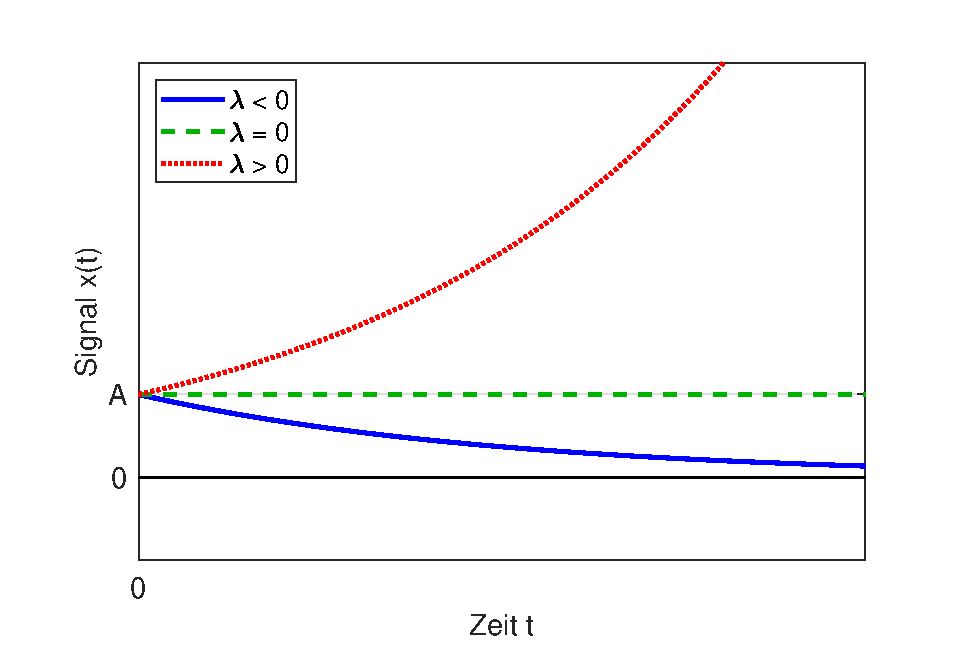
\includegraphics[width=0.5\textwidth]{Kapitel2/Bilder/image24.eps}}
  \caption{Anregung eines RC-Glieds mit einem Rechtecksignal}
  \label{fig:inconnue}
\end{figure}

\noindent Nach der Anregung klingt das Ausgangssignal ab und erreicht f\"{u}r t $\rightarrow$ $\mathrm{\infty}$ den Wert null.\bigskip

\noindent
\colorbox{lightgray}{%
\arrayrulecolor{white}%
\renewcommand\arraystretch{0.6}%
\begin{tabular}{ wl{16.5cm} }
{\fontfamily{phv}\selectfont
\noindent
Beispiel: Integrierer als grenzstabiles System}
\end{tabular}%
}\bigskip

\noindent Als Beispiel für ein grenzstabiles System wird ein Integrierer hinsichtlich seiner Stabilität bewertet. Er besitzt die Impulsantwort

\begin{equation}\label{eq:threehundredeightynine}
g\left(t\right)=\int\limits _{-\infty }^{t}\delta \left(\tau \right) \;\tau =\sigma \left(t\right)
\end{equation}

\noindent Die Impulsantwort besitzt f\"{u}r t $\rightarrow$ $\mathrm{\infty}$ den konstanten Wert g${}_{0}$ = 1, das System ist demnach grenzstabil. Wird als Eingangssignal ein Rechtecksignal 

\begin{equation}\label{eq:threehundredninety}
u\left(t\right)=\sigma \left(t\right)-\sigma \left(t-2\right)
\end{equation}

\noindent gewählt, ergibt sich das Ausgangssignal durch grafische Faltung zu

\begin{equation}\label{eq:threehundredninetyone}
y\left(t\right)=t\cdot \sigma \left(t\right)-\left(t-2\right)\cdot \sigma \left(t-2\right)
\end{equation}

\noindent Bild \ref{fig:FaltungIntegrierer} zeigt die Antwort y(t) des Integrierers auf das Rechteck-Signal am Eingang.

\begin{figure}[H]
  \centerline{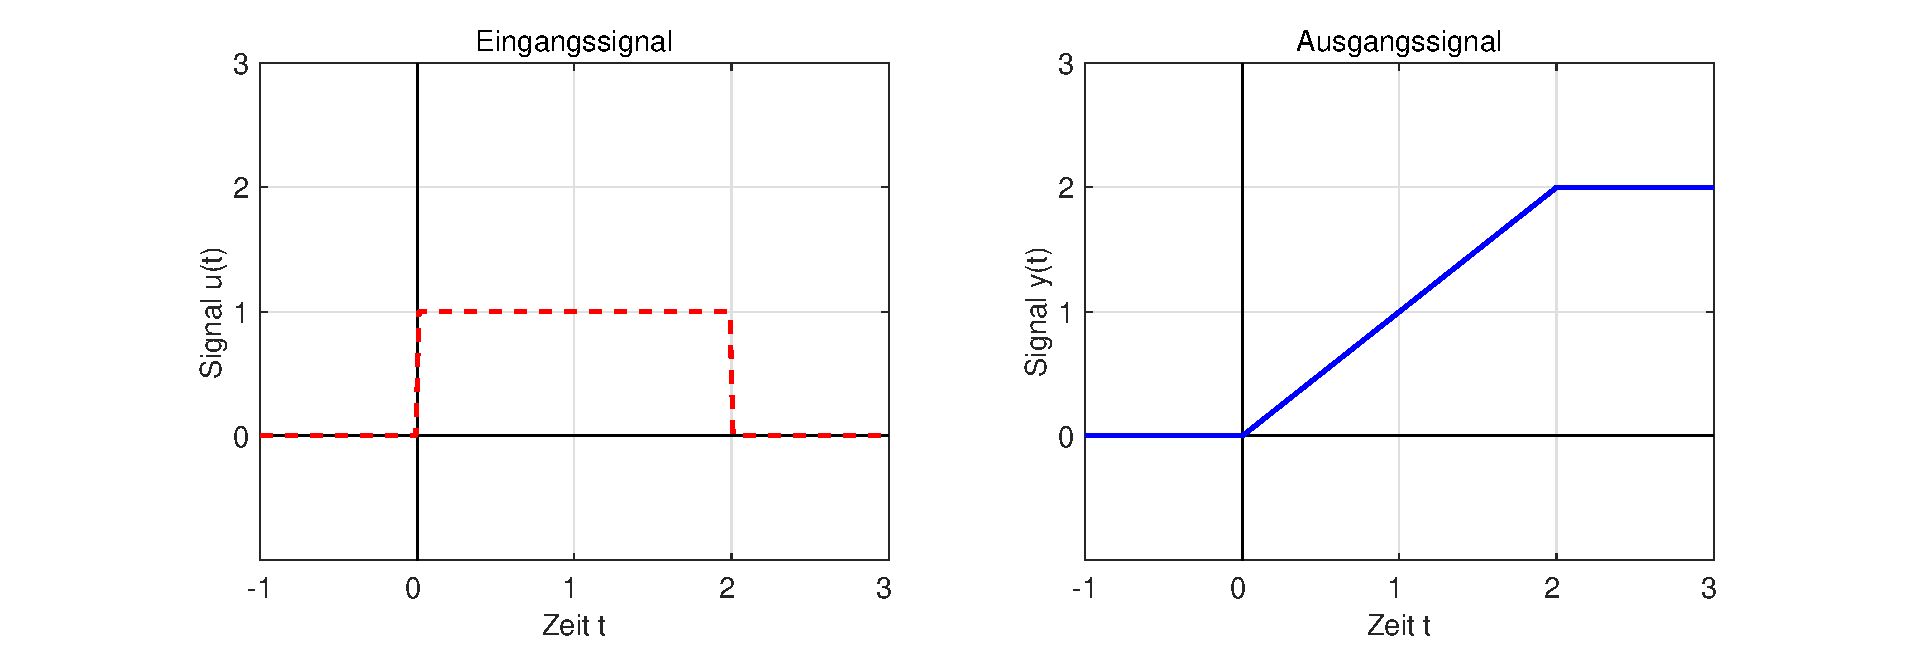
\includegraphics[width=1\textwidth]{Kapitel2/Bilder/image25}}
  \caption{Verhalten eines Integrierers als Beispiel für ein grenzstabiles System}
  \label{fig:FaltungIntegrierer}
\end{figure}

\noindent Wird das Eingangssignal zeitlich begrenzt, besitzt der Integrierer ein endliches Ausgangssignal. Damit ist bestätigt, dass der Integrierer ein grenzstabiles System ist. 


\subsection{Simulation linearer, zeitinvarianter Systeme}

\noindent Die Beschreibung dynamischer Systeme kann über mathematische Funktionen erfolgen. Die analytische Berechnung von Systemreaktionen ist wichtig, um Systeme zu interpretieren und zu charakterisieren.
Ihre Berechnung wird bei Systemen höherer Ordnung jedoch zumindest aufwendig. Neben der analytischen Berechnung werden deshalb numerische Verfahren zur Simulation des Systemverhaltens eingesetzt.\newline
Eine zeitdiskrete Approximation zeitkontinuierlicher Systeme wird in Teil B dieser Buchreihe behandelt. Dort werden nach Einführung des Abtasttheorems das Forward- und Backward-EulerVerfahren sowie die bilineare Transformation beschrieben. Um vorab das Verhalten zeitkontinuierlicher Systeme simulieren zu können, werden Systeme mit Blockdiagrammen beschrieben und ihre
Systemreaktion mit MATLAB / Simulink berechnet.

\subsubsection{Beschreibung von Systemen mit Blockdiagrammen} \label{threefiveone}

\noindent Die Systembeschreibung mit Blockdiagrammen geht von einer Differentialgleichung der Form

\begin{equation}\label{eq:threehundredninetytwo}
a_{0}\cdot y(t) + a_{1}\cdot \frac{dy}{dt}+a_{2}\cdot \frac{d^2y}{dt^2}+ ... +a_{n}\cdot \frac{d^Ny}{dt^N}=
b_{0}\cdot u(t) + b_{1}\cdot \frac{du}{dt}+b_{2}\cdot \frac{d^2u}{dt^2}+ ... +b_{m}\cdot \frac{d^Mu}{dt^M}
\end{equation}

\noindent mit entsprechenden Anfangsbedingungen aus. Eine Möglichkeit der Realisierung ergibt sich durch eine
Darstellung mit Differenzierern. Diese Darstellungsform hat drei entscheidende Nachteile:

\begin{itemize}
    \item Das Eingangssignal muss bei einigen Anwendungen abgeleitet werden. Handelt es sich um
einen Signalsprung am Eingang, ist die Ableitung ein Impuls. Er lässt sich numerisch nicht
realisieren.
    \item Ein idealer Differenzierer ist kein kausales System und kann deshalb nicht realisiert werden.
    \item Reale analoge Signale weisen Rauschen auf, das typischerweise schnell veränderliche Anteile
besitzt. Differenzierer verstärken diese schnell veränderlichen Rauschanteile. Eine
Systemrealisierung mit Differenzierern ist deshalb wenig robust.
\end{itemize}

\noindent Im Gegensatz zu Differenzierern wirken Integrierer glättend. Eine Darstellung von dynamischen
Systemen mit Integrieren führt damit zu besseren und robusteren Realisierungen, was insbesondere bei
der späteren Umsetzung der Systembeschreibung in reale Systeme von Bedeutung ist. Deshalb werden zur Beschreibung von Systemen mit Blockdiagrammen Integrierer eingesetzt. Ausgehend von der Systembeschreibung mit einer Differentialgleichung wird im Folgenden ein entsprechendes Blockschaltbild auf zwei unterschiedlichen Wegen hergeleitet. Bei beiden Varianten wird davon ausgegangen, dass das System kausal ist. Für kausale Systeme gilt die Bedingung N $\geqslant$ M.\bigskip

{\fontfamily{phv}\selectfont
\noindent\textbf{Grafisch motivierte Herleitung des Blockschaltbildes von LTI-Systemen }}

\noindent Um die Differentialgleichung in eine Integralgleichung zu überführen, muss eine N-fache Integration der Differentialgleichung (\ref{eq:threehundredninetytwo}) durchgeführt werden. 

\begin{equation}\label{eq:threehundredninetythree}
\begin{split}
a_{0} \cdot \int\limits _{-\infty }^{t}\ldots \int\limits _{-\infty }^{\tau _{3}}\int\limits _{-\infty }^{\tau _{2} }y\left(\tau _{1} \right) \; d\tau _{1}  \; d\tau _{2} \cdots d\tau _{N}  \; +a_{1} \cdot \int\limits _{-\infty }^{t}\ldots \int\limits _{-\infty }^{\tau _{3} }\int\limits _{-\infty }^{\tau _{2} }y\left(\tau _{1} \right) \; d\tau _{1}  \; d\tau _{2} \cdots d\tau _{N-1}  +...+a_{N} \cdot y\left(t\right)\\
= 0 \cdot \int\limits _{-\infty }^{t}\ldots \int _{-\infty }^{\tau _{3} }\int\limits _{-\infty }^{\tau _{2} }u\left(\tau _{1} \right) \; d\tau _{1}  \; d \tau _{2} \cdots d\tau _{N}  +...+b_{M} \cdot \int\limits _{-\infty }^{t}\ldots \int _{-\infty }^{\tau _{3} }\int\limits _{-\infty }^{\tau _{2} }u\left(\tau _{1} \right) \; d\tau _{1}  \;d\tau _{2} \cdots d\tau _{N-M}
\end{split}
\end{equation}

\noindent Die Gleichung kann nach y(t) aufgelöst werden. Es ergibt sich die Systemdarstellung 

\begin{equation}\label{eq:threehundredninetyfour}
\begin{split}
y\left(t\right) & = \frac{1}{a_{N} } \cdot \left(b_{0} \cdot \int\limits _{-\infty }^{t}\ldots \int\limits _{-\infty }^{\tau _{3} }\int\limits _{-\infty }^{\tau _{2} }u\left(\tau _{1} \right) \; d\tau _{1}  \; d\tau _{2} \cdots {\rm d}\tau _{N}  +...+b_{M} \cdot \int\limits _{-\infty }^{t}\ldots \int\limits _{-\infty }^{\tau _{3} }\int\limits _{-\infty }^{\tau _{2} }u\left(\tau _{1} \right) \; d\tau _{1}  \; d\tau _{2} \cdots d\tau _{N-M}  \right) \\ 
& +\frac{1}{a_{N} } \cdot \left(-a_{0} \cdot \int\limits _{-\infty }^{t}\ldots \int\limits _{-\infty }^{\tau _{3} }\int\limits _{-\infty }^{\tau _{2} }y\left(\tau _{1} \right) \; d\tau _{1}  \; d\tau _{2} \cdots {\rm d}\tau _{N}  \;-...-a_{N-1} \cdot \int\limits _{-\infty }^{t}y\left(\tau _{1} \right) \; d\tau _{1} \right)
\end{split}
\end{equation}

\noindent In Gleichung \eqref{eq:threehundredninetyfour} wird von einer Integration ausgegangen, die bei t = - $\mathrm{\infty}$ beginnt. Numerische Simulationen beginnen jedoch an einem festen Zeitpunkt t${}_{0}$, typischerweise zum Zeitpunkt t${}_{0}$ = 0. Damit m\"{u}ssen bei der Integration die Anfangsbedingungen ber\"{u}cksichtigt werden. 

\begin{equation}\label{eq:threehundredninetyfive}
y\left(t\right)=\int\limits _{-\infty }^{t}u\left(\tau \right) \; d\tau =\int\limits _{t_{0} }^{t}u\left(\tau \right) \; d\tau +\int\limits _{-\infty }^{t_{0} }u\left(\tau \right) \; d\tau =\int\limits _{t_{0} }^{t}u\left(\tau \right) \; d\tau +y(t_{0} )=\int\limits _{0}^{t}u\left(\tau \right) \; d\tau +y(0)
\end{equation}

\noindent Die Anfangsbedingung wird bei der Simulation auf Englisch als sogenannte \textit{Initial Condition} angegeben.\bigskip

\noindent
\colorbox{lightgray}{%
\arrayrulecolor{white}%
\renewcommand\arraystretch{0.6}%
\begin{tabular}{ wl{16.5cm} }
{\fontfamily{phv}\selectfont
\noindent
Beispiel: Beschreibung eines Feder-Masse-Dämpfer-Systems in integraler Form}
\end{tabular}%
}\bigskip

\noindent Die N-fache Integration einer Differentialgleichung f\"{u}hrt zu un\"{u}bersichtlichen Gleichungen. Deshalb wird das Verfahren an einem Feder-Masse-D\"{a}mpfer-System veranschaulicht, das zum Zeitpunkt t = 0 die Auslenkung x${}_{0}$ und die Geschwindigkeit v${}_{0}$ besitzt. Eingangsgr\"{o}{\ss}e ist die Kraft F${}_{E}$(t), Ausgangsgr\"{o}{\ss}e ist die Auslenkung x(t). 

\begin{equation}\label{eq:threehundredninetysix}
F_{E} \left(t\right)=m\cdot \frac{d^{2} x}{dt^{2} } +D\cdot \frac{dx}{dt} +c\cdot x\left(t\right)
\end{equation}

\noindent Integration nach der Zeit f\"{u}hrt mit t${}_{0}$ = 0 zu dem Ausdruck

\begin{equation}\label{eq:threehundredninetyseven}
F_{E} \left(t\right)= LONG
\end{equation}

\noindent Bei erneuter Integration ergibt sich die Gleichung 

\begin{equation}\label{eq:threehundredninetyeight}
LONG
\end{equation}

\noindent Auflösen nach x(t) ergibt die Systembeschreibung des Feder-Masse-Dämpfer-Systems in Integralform

\begin{equation}\label{eq:threehundredninetynine}
LONG
\end{equation}\bigskip

\noindent Die Systembeschreibung in Integralform kann als Blockdiagramm dargestellt werden. Dabei wird eine Verstärkung mit einem Zahlenwert an der Linie dargestellt, Summationspunkte über Kreise und einzelne Übertragungsglieder in einem Rechteck. Das Rechteck mit einem Integralzeichen stellt einen idealen Integrierer dar. Pfeile geben die Flussrichtung des Signals an. Bild \ref{fig:ZeitinvarianzBSB} stellt das lineare zeitinvariante System als Blockschaltbild in der sogenannten Direktstruktur dar.

\begin{figure}[H]
  \centerline{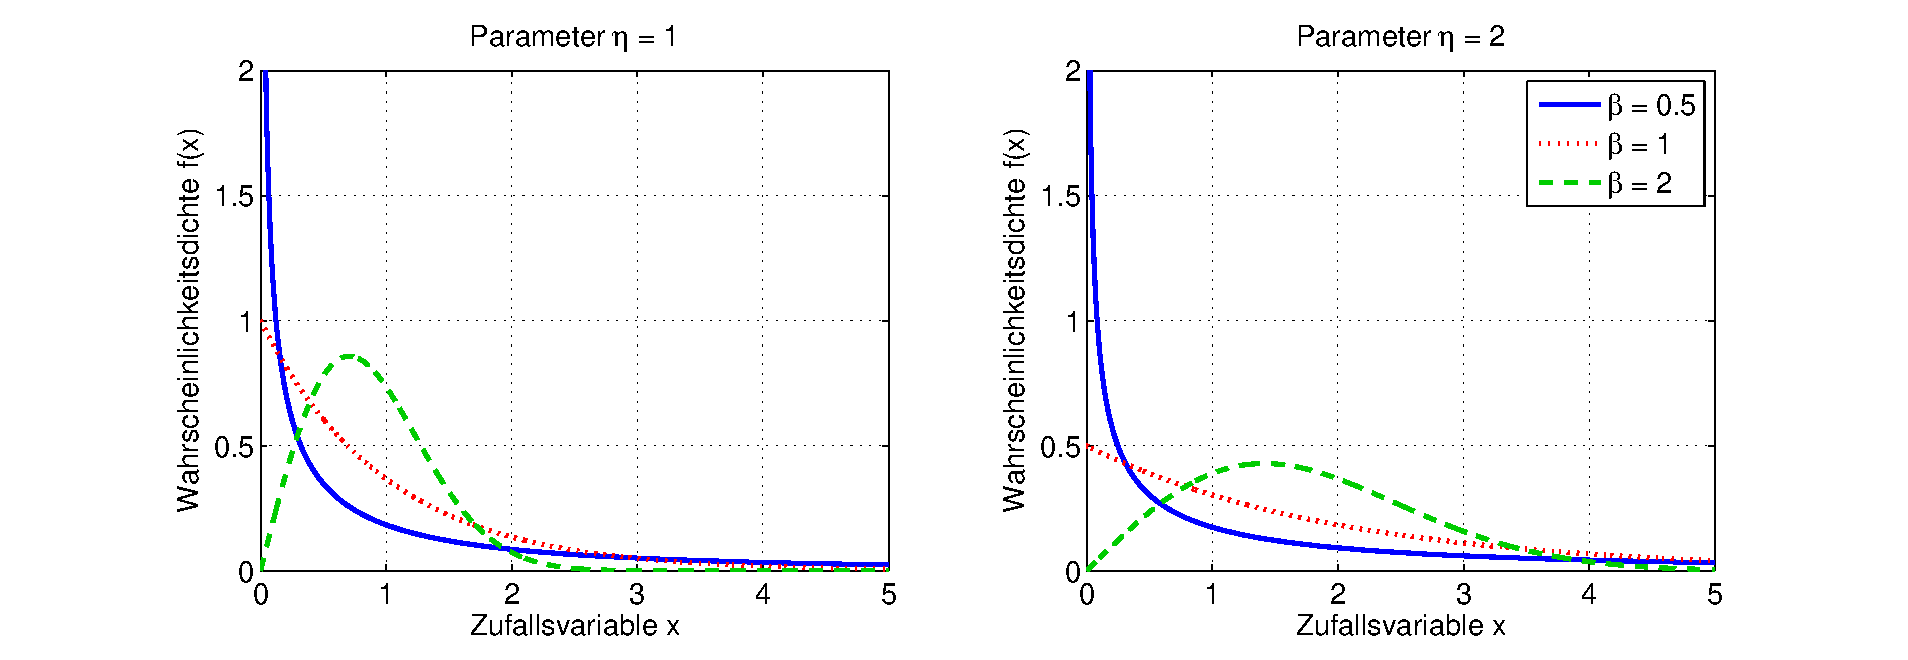
\includegraphics[width=0.5\textwidth]{Kapitel2/Bilder/image26}}
  \caption{Blockschaltbild eines linearen, zeitinvarianten Systems}
  \label{fig:ZeitinvarianzBSB}
\end{figure}

\noindent Die Direktstruktur ergibt sich unmittelbar aus der Differentialgleichung (\ref{eq:threehundredninetyfour}), die Koeffizienten an und b$_{m}$ entsprechen denen der Differentialgleichung. Bei dieser Darstellung ergibt sich das Problem, dass 2$\cdot$N Integrierer zur Systemrealisierung notwendig sind. Unter der Voraussetzung, dass das System ein lineares, zeitinvariantes System ist, ist eine Vertauschung der Funktionsblöcke möglich. Dieser
Sachverhalt wird nach der Beschreibung von LTI-Systemen im Laplace-Bereich noch einmal aufgegriffen. Nach Austauschen der Reihenfolge der Strukturen ergibt sich das in Bild \ref{fig:ZeitinvarianzBSBMitTausch} 3.27 dargestellte Blockschaltbild.

\begin{figure}[H]
  \centerline{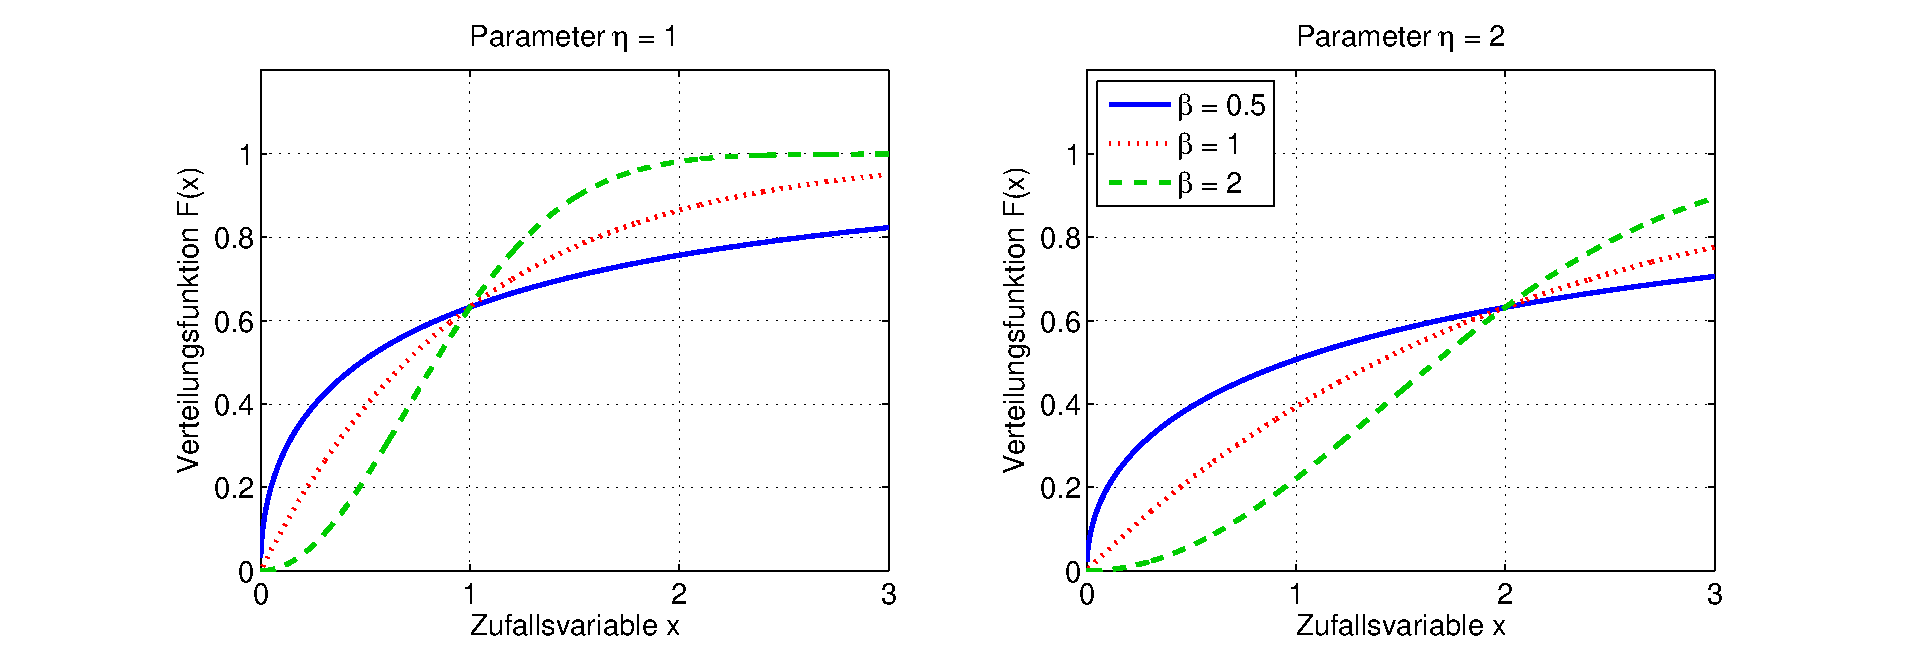
\includegraphics[width=0.5\textwidth]{Kapitel2/Bilder/image27}}
  \caption{Blockschaltbild eines linearen, zeitinvarianten Systems mit vertauschter Blockreihenfolge}
  \label{fig:ZeitinvarianzBSBMitTausch}
\end{figure}

\noindent Die beiden Pfade der Integrierer haben dieselben Eingangssignale, sie können ohne Veränderung derSystemfunktion zusammengefasst werden. Es ergibt sich das in Bild \ref{fig:KanonischZeitinvarianzBSB} dargestellte Blockschaltbild.

\begin{figure}[H]
  \centerline{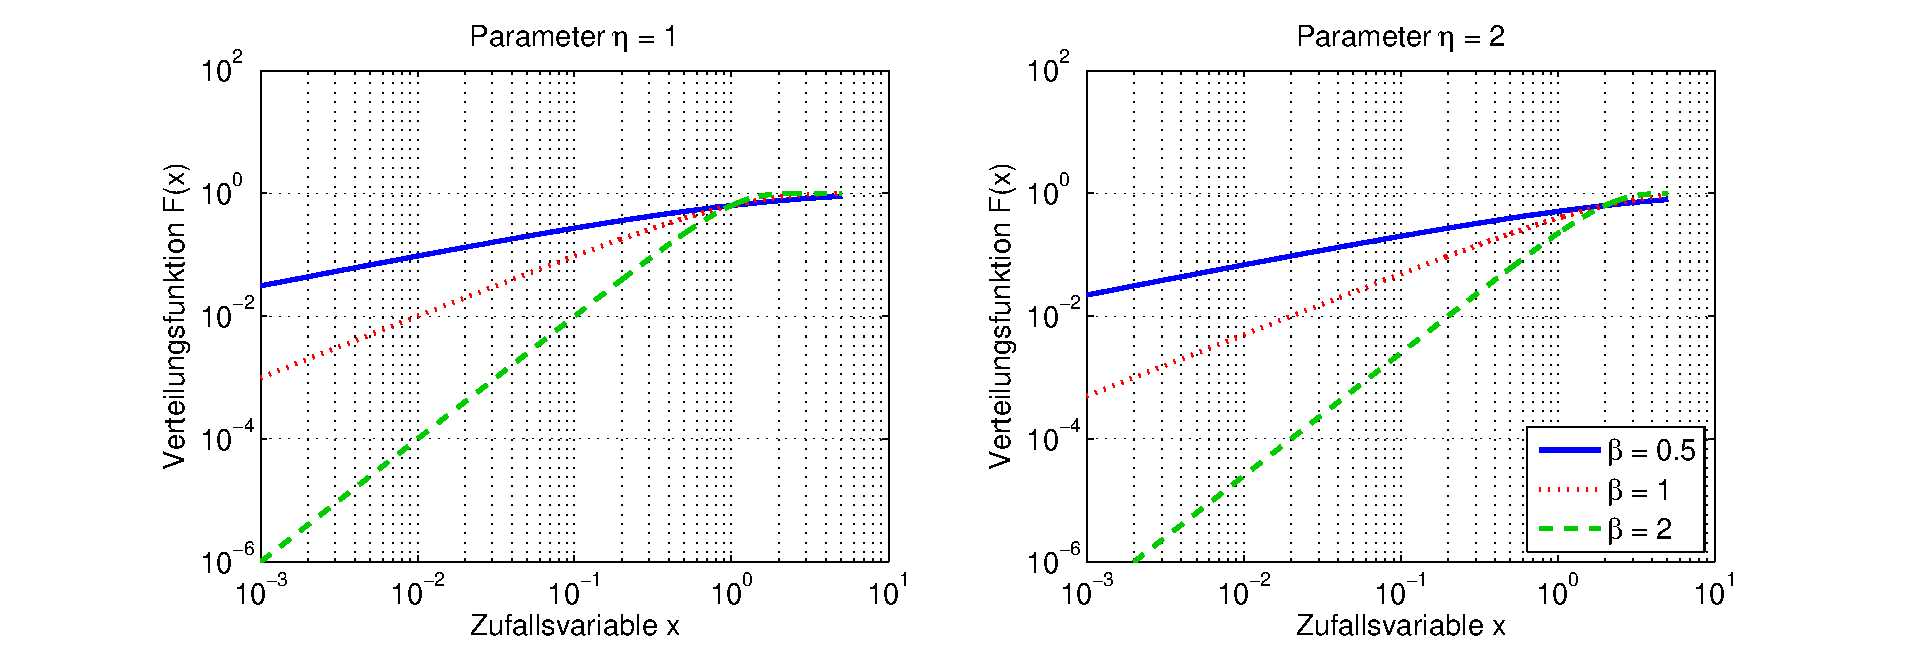
\includegraphics[width=0.5\textwidth]{Kapitel2/Bilder/image28}}
  \caption{Kanonisches Blockschaltbild eines linearen, zeitinvarianten Systems}
  \label{fig:KanonischZeitinvarianzBSB}
\end{figure}

\noindent Das System wird mit N Integrierern beschrieben. Es kann gezeigt werden, dass das System nicht mit weniger als N Integrierern realisiert werden kann. Die Darstellung wird deshalb als kanonisches Blockschaltbild bezeichnet.\bigskip

{\fontfamily{phv}\selectfont
\noindent\textbf{Mathematische motivierte Herleitung des Blockschaltbildes von LTI-Systemen}}

\noindent Auch die mathematisch orientierte Herleitung von Blockschaltbildern basiert auf der
Differentialgleichung

\begin{equation}\label{eq:threetwohundred}
a_{0}\cdot y(t) + a_{1}\cdot \frac{dy}{dt}+a_{2}\cdot \frac{d^2y}{dt^2}+ ... +a_{n}\cdot \frac{d^Ny}{dt^N}=
b_{0}\cdot u(t) + b_{1}\cdot \frac{du}{dt}+b_{2}\cdot \frac{d^2u}{dt^2}+ ... +b_{m}\cdot \frac{d^Mu}{dt^M}
\end{equation}

\noindent mit den entsprechenden Anfangsbedingungen. Das System kann in zwei Anteile zerlegt werden, die Eingangsgröße u(t) und ihre Ableitungen sowie die Ausgangsgröße y(t) und ihre Ableitungen. Die Gleichung kann in zwei Stufen aufgeteilt werden. Zunächst werden Linearkombinationen der Eingangsgröße und ihren Ableitungen gebildet.

\begin{equation}\label{eq:threetwohundredone}
x(t) = b_{0}\cdot u(t) + b_{1}\cdot \frac{du}{dt} +  b_{2}\cdot \frac{d^2u}{dt^2} + \cdots + b_{M}\cdot \frac{d^Mu}{dt^M}
\end{equation}

\noindent Anschließend wird eine Linearkombination der Ausgangsgröße y(t) und ihren Ableitungen berechnet und x(t) gleichgesetzt.

\begin{equation}\label{eq:threetwohundredtwo}
a_{0}\cdot y(t) + a_{1}\cdot \frac{dy}{dt}+a_{2}\cdot \frac{d^2y}{dt^2}+ ... +a_{n}\cdot \frac{d^Ny}{dt^N} = x(t)
\end{equation}

\noindent Grafisch sind diese Operationen in Bild 3.29 dargestellt.

\begin{figure}[H]
  \centerline{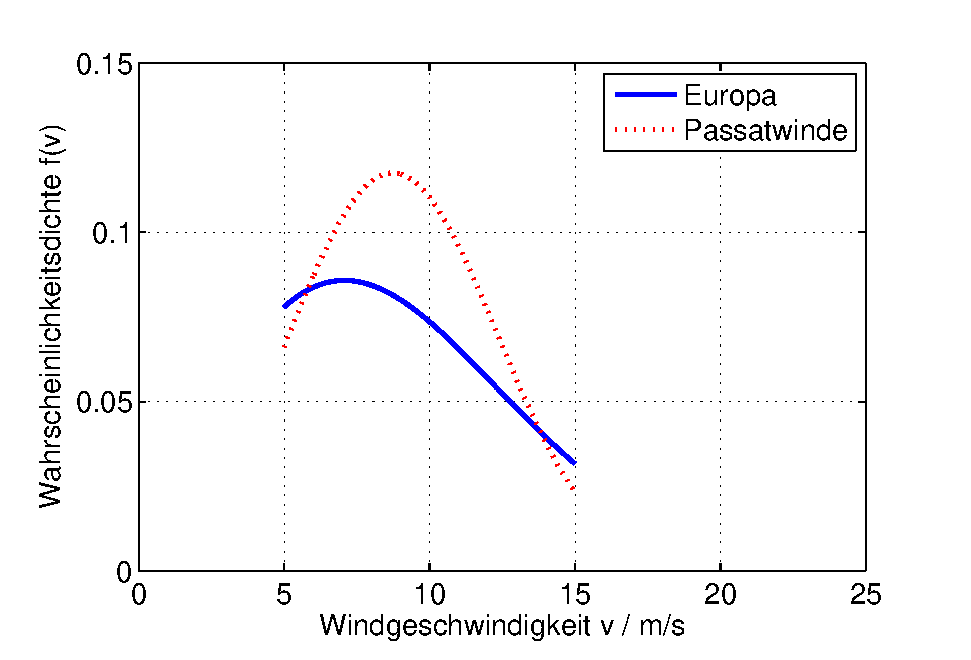
\includegraphics[width=0.5\textwidth]{Kapitel2/Bilder/image29}}
  \caption{Zerlegung eines Systems in zwei Teilsysteme bei variierter Reihenfolge der Funktionsblöcke}
  \label{fig:Zerlegung}
\end{figure}

\noindent Für das LTI-System ist die Reihenfolge der beiden Funktionsblöcke unerheblich, sodass die beiden Darstellungen in Bild \ref{fig:Zerlegung} äquivalent sind. Bei geänderter Reihenfolge gelten mit den Bezeichnungen in Bild \ref{fig:Zerlegung}  die Gleichungen

\begin{equation}\label{eq:threetwohundredthree}
a_{0}\cdot z(t) + a_{1}\cdot \frac{dz}{dt}+a_{2}\cdot \frac{d^2z}{dt^2}+ ... +a_{n}\cdot \frac{d^Nz}{dt^N} = u(t)
\end{equation}

\noindent und

\begin{equation}\label{eq:threetwohundredfour}
y(t) = b_{0}\cdot z(t) + b_{1}\cdot \frac{dz}{dt} + b_{2}\cdot \frac{d^2z}{dt^2} + \cdots + b_{M}\cdot \frac{d^Mz}{dt^M} 
\end{equation}

\noindent Die N-fache Integration von Gleichung (\ref{eq:threetwohundredthree})

\begin{equation}\label{eq:threetwohundredfive}
\begin{split}
& a_{0}\cdot \int\limits _{-\infty }^{t} \cdots  \int\limits _{-\infty }^{t_{3}}  \int\limits _{-\infty }^{t_{2}} z(\tau _{1}) d\tau _{1} d\tau _{2} \cdots d\tau _{N} + a_{1}\cdot \int\limits _{-\infty }^{t} \cdots  \int\limits _{-\infty }^{t_{3}}  \int\limits _{-\infty }^{t_{2}} z(\tau _{1}) d\tau _{1} d\tau _{2} \cdots d\tau _{N-1} + \cdots + a_{N} \cdot z(t)\\ 
& = \int\limits _{-\infty }^{t} \cdots  \int\limits _{-\infty }^{t_{3}} \int\limits _{-\infty }^{t_{2}} u(\tau _{1}) d\tau _{1} d\tau _{2} \cdots d\tau _{N}     
\end{split}
\end{equation}

\noindent und Auflösen nach z(t) führt zu dem Ausdruck

\begin{equation}\label{eq:threetwohundredsix}
\begin{split}
z(t) & = \frac{1}{a_{N}}\cdot  \int\limits _{-\infty }^{t} \cdots  \int\limits _{-\infty }^{\tau_{3}}  \int\limits _{-\infty }^{\tau_{2}} u(\tau _{1}) d\tau _{1} d\tau _{2} \cdots d\tau _{N} \\
 & - \frac{a_{0}}{a_{N}}\cdot\int\limits _{-\infty }^{t} \cdots  \int\limits _{-\infty }^{\tau_{3}}  \int\limits _{-\infty }^{\tau_{2}} z(\tau _{1}) d\tau _{1} d\tau _{2} \cdots d\tau _{N} - \cdots - \frac{a_{N-1}}{a_{N}}\cdot \int\limits _{-\infty }^{\tau_{2}} z(\tau _{N-1}) d\tau _{N-1}
\end{split}
\end{equation}	

\noindent Bild \ref{fig:BlockschaltbildTeilsystem} stellt diese Gleichung als Blockdiagramm dar.

\begin{figure}[H]
  \centerline{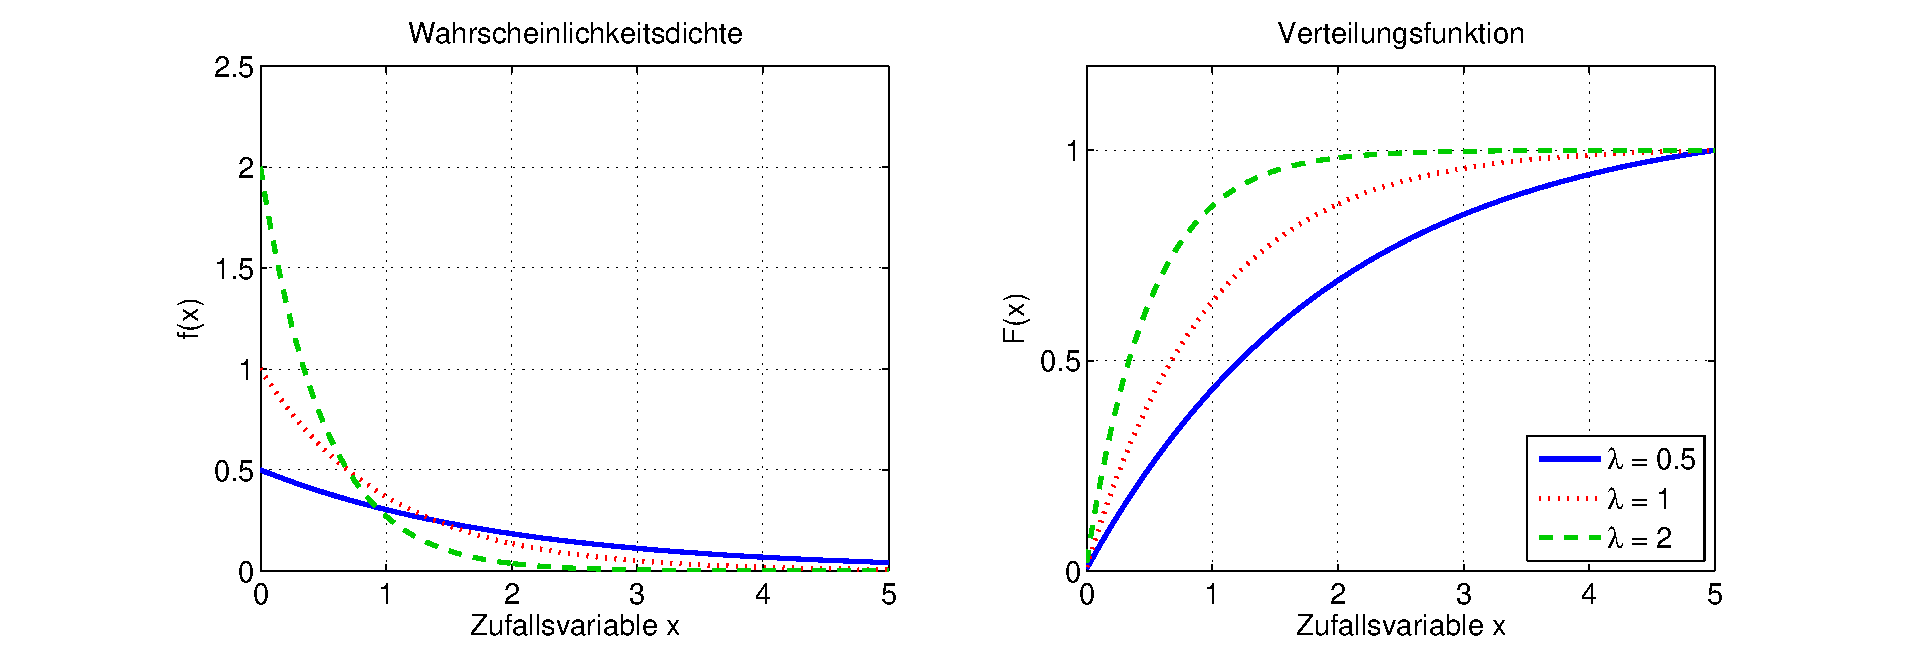
\includegraphics[width=0.4\textwidth]{Kapitel2/Bilder/image30}}
  \caption{Blockschaltbild des in Gleichung (\ref{eq:threetwohundredsix}) beschriebenen Teilsystems}
  \label{fig:BlockschaltbildTeilsystem}
\end{figure}

\noindent Das Ausgangssignal y(t) setzt sich nach Gleichung (\ref{eq:threetwohundredfour}) aus einer Linearkombination von Ableitungen der Größe z(t) zusammen.

\begin{equation}\label{eq:threetwohundredseven}
y(t) = b_{0}\cdot z(t) + b_{1}\cdot \frac{dz}{dt} + b_{2}\cdot \frac{d^2z}{dt^2} + \cdots + b_{M}\cdot \frac{d^Mz}{dt^M} 
\end{equation}

\noindent Die Eingangssignale der Integrierer sind Ableitungen der Größe z(t). Damit kann das Gesamtsystem mit dem Blockschaltbild in Bild (\ref{fig:BlockschaltbildZeitinvariant}) beschreiben werden.

\begin{figure}[H]
  \centerline{\includegraphics[width=0.7\textwidth]{Kapitel2/Bilder/image31}}
  \caption{Blockschaltbild eines linearen, zeitinvarianten Systems}
  \label{fig:BlockschaltbildZeitinvariant}
\end{figure}

\noindent In technischen Systemen gilt oftmals die Beziehung M < N, in diesem Fall sind die entsprechenden Koeffizienten b$_{m}$ zu null zu setzen.
Beide Herleitungen führen zu einem kanonischen Blockschaltbild mit N Integrierern. Bei der Integration müssen die Anfangsbedingungen in Form von \textit{Initial Conditions} berücksichtigt werden.

\bigskip

\noindent
\colorbox{lightgray}{%
\arrayrulecolor{white}%
\renewcommand\arraystretch{0.6}%
\begin{tabular}{ wl{16.5cm} }
{\fontfamily{phv}\selectfont
\noindent
Beispiel: Darstellung des Feder-Masse-Dämpfer-Systems als Blockschaltbild}
\end{tabular}%
}\bigskip

\noindent Die Anwendung der Systemdarstellung über Blockschaltbilder wird anhand eines Feder-Masse-
Dämpfer-Systems verdeutlicht.

\begin{equation}\label{eq:threetwohundredeight}
F_{E} \left(t\right)=m\cdot \frac{d^{2} x}{dt^{2} } +D\cdot \frac{dx}{dt} +c\cdot x\left(t\right)
\end{equation}

\noindent Eingangssignal ist der Kraftverlauf F$_{E}$(t), Ausgangssignal ist die Auslenkung x(t). Einsetzen der
entsprechenden Koeffizienten in die allgemeine Form führt zu der Darstellung des Systems als kanonisches Blockschaltbild. Es ist in Bild \ref{fig:BlockschaltbilFDM} dargestellt.

\begin{figure}[H]
  \centerline{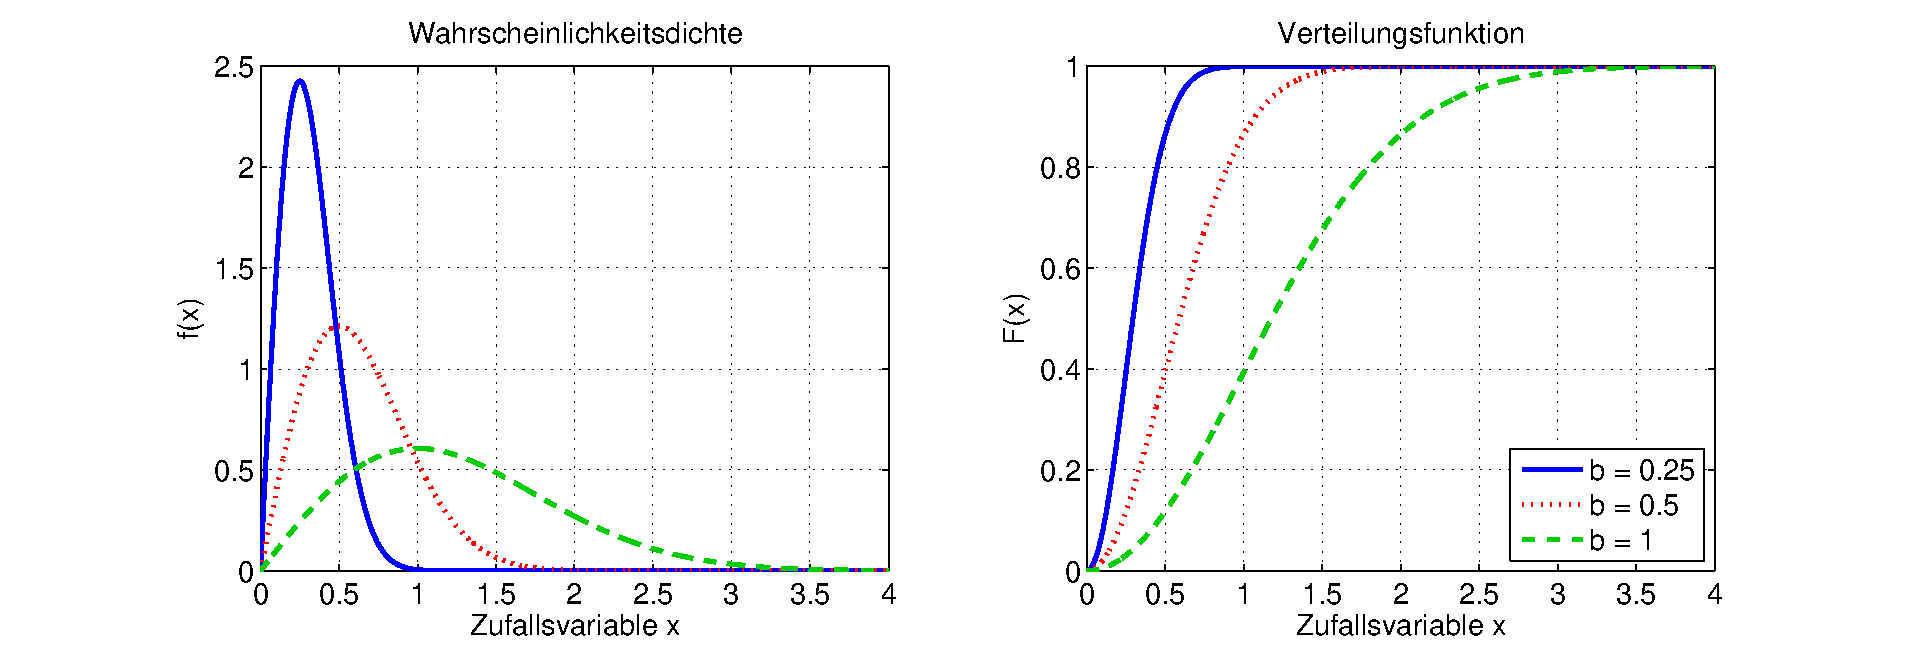
\includegraphics[width=0.5\textwidth]{Kapitel2/Bilder/image32}}
  \caption{Kanonisches Blockschaltbild eines Feder-Masse-Dämpfer-Systems}
  \label{fig:BlockschaltbilFDM}
\end{figure}

\noindent Diese Darstellung kann anschaulich interpretiert werden. Das Ausgangssignal des zweiten Integrierers ist die Auslenkung x(t) des Systems. Damit ist das Eingangssignal des zweiten Integrierers die erste Ableitung dx/dt und das Eingangssignal des ersten Integrierers die zweite Ableitung d²x/dt² der Auslenkung x(t). Nach Gleichung (\ref{eq:threetwohundredeight}) gilt für die zweite Ableitung

\begin{equation}\label{eq:threetwohundrednine}
\frac{d^{2} x}{dt^{2}} = \frac{1}{m} \cdot (F_{E}(t) - D\cdot \frac{dx}{dt} - c\cdot x\left(t\right))
\end{equation}

\noindent Eine Analyse des Signalflusses zeigt, dass das Blockschaltbild genau diese Struktur realisiert. Die
Anfangsbedingungen der beiden Integrierer ergeben sich aus x(t$_{0}$) und dx/dt an der Stelle t = t$_{0}$.

\subsubsection{Simulation von Systemen mit MATLAB / Simulink}

\noindent Das in Abschnitt \ref{threefiveone} beschriebene Blockschaltbild kann zur Simulation des Systems in Simulink verwendet werden. Dabei wird das Blockdiagramm in Simulink grafisch programmiert. Simulink stellt verschiedene elementare Übertragungsglieder zur Verfügung.\medskip

{\fontfamily{phv}\selectfont
\noindent\textbf{Signalquellen}}

\noindent Mithilfe von Signalquellen (\textit{Sources}) werden Eingangssignale generiert. Neben den typischen Signalformen wie Sprung-, Rampen-, Rechteck- und Sinusfunktion erlaubt Simulink die Erzeugung von Signalquellen über selbst definierte Variablen oder sogenannte mat-Files. Damit ist es zum Beispiel auch möglich, gemessene Daten als Signalquelle zu verwenden, indem die Messdaten aus mat-Files eingelesen werden. Tabelle \ref{tab:threeeleven} stellt eine Auswahl von Signalquellen in Simulink dar.

\clearpage

\begin{table}[H]
\caption{Auswahl von Signalquellen in Simulink}
\setlength{\fboxsep}{0pt}%
\colorbox{lightgray}{%
\arrayrulecolor{white}%
\begin{tabular}{| c | c | c | c |}
\hline
\parbox[c][0.28in][c]{1.6in}{\smallskip\centering\textbf{\fontfamily{phv}\selectfont{Signalquelle}}} & \parbox[c][0.28in][c]{1.5in}{\smallskip\centering\textbf{\fontfamily{phv}\selectfont{Simulink Symbol}}} &
\parbox[c][0.28in][c]{1.6in}{\smallskip\centering\textbf{\fontfamily{phv}\selectfont{Signalquelle}}} &
\parbox[c][0.28in][c]{1.5in}{\smallskip\centering\textbf{\fontfamily{phv}\selectfont{Simulink Symbol}}}\\ \hline


\parbox[c][0.9in][c]{1.6in}{\centering{\fontfamily{phv}\selectfont{Konstante}}} &
\parbox[c][0.9in][c]{1.5in}{\centerline{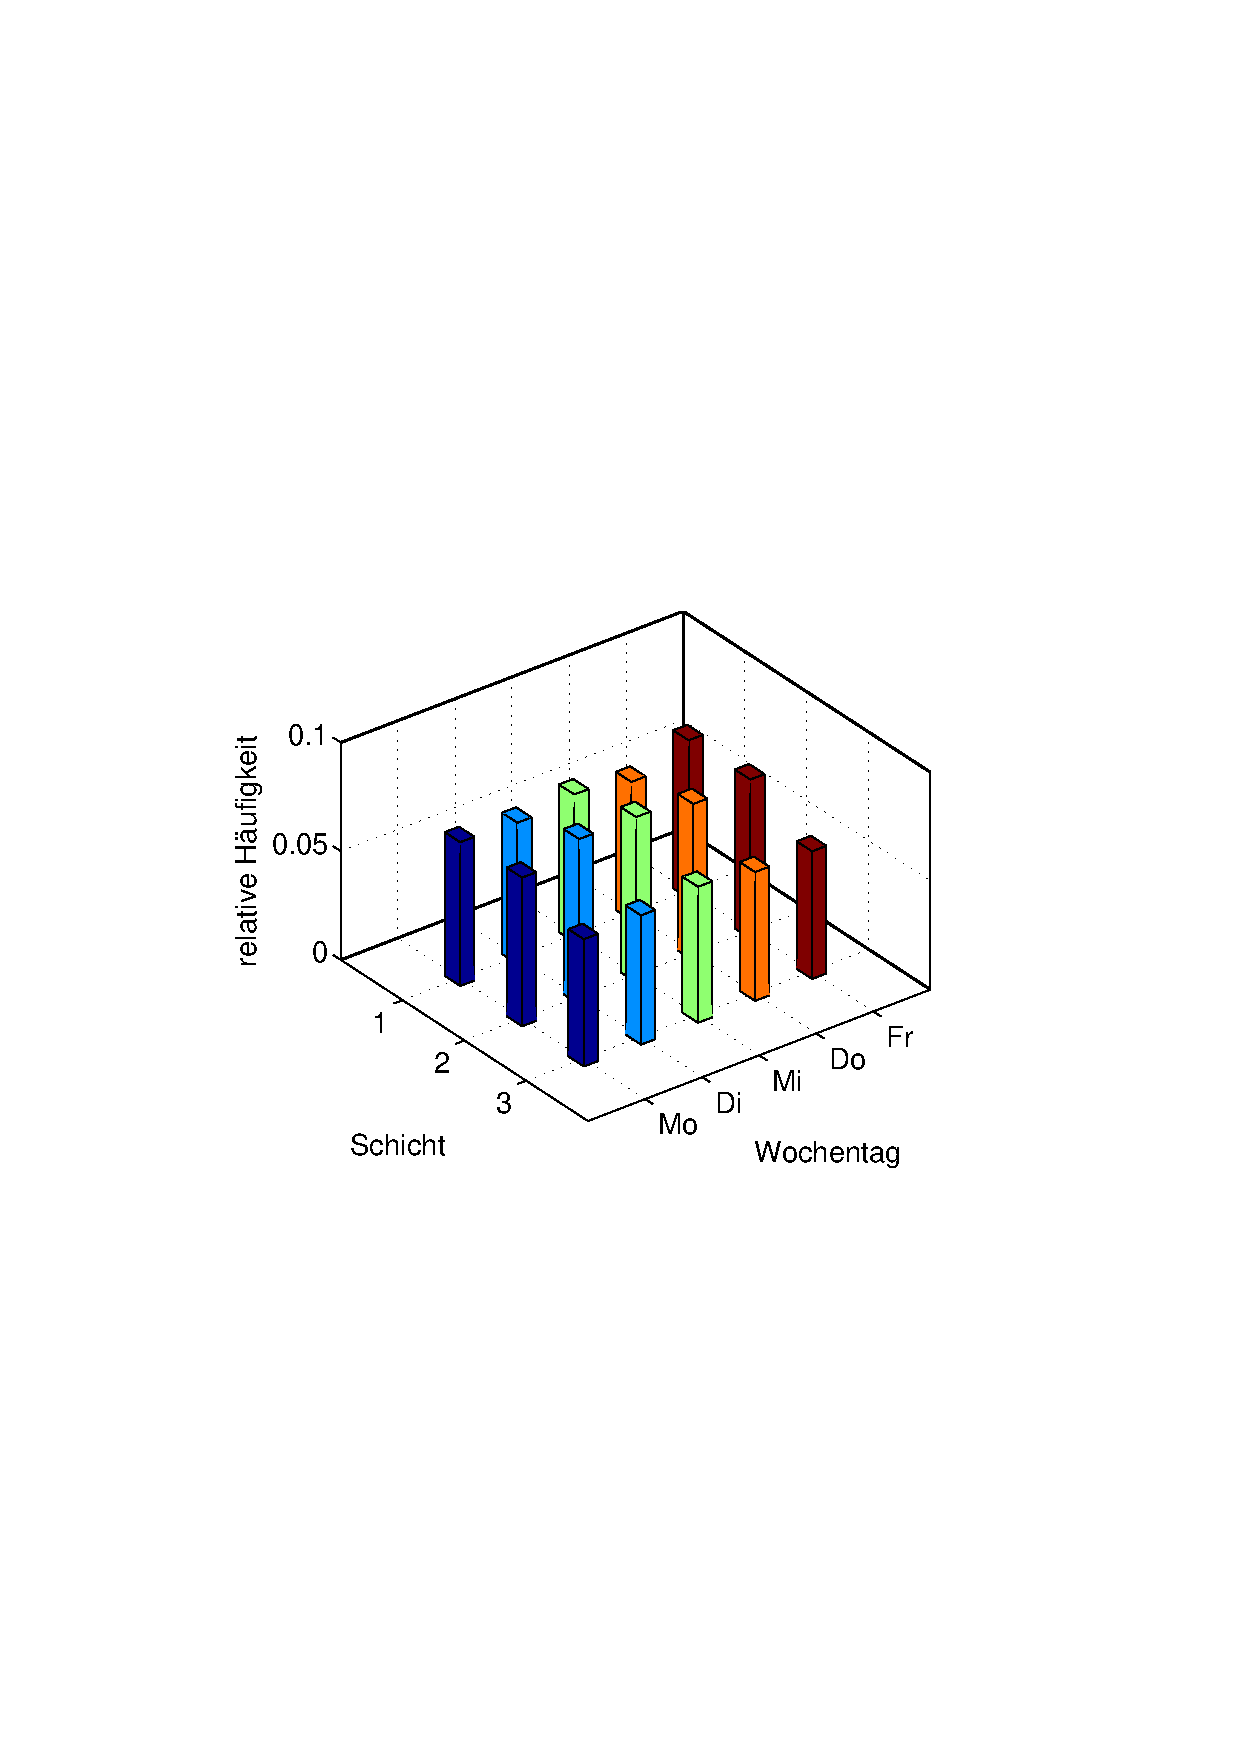
\includegraphics[width=0.1\textwidth]{Kapitel2/Table/image1.png}}} &
\parbox[c][0.9in][c]{1.6in}{\centering{\fontfamily{phv}\selectfont{Sinusfunktion}}} &
\parbox[c][0.9in][c]{1.5in}{\centerline{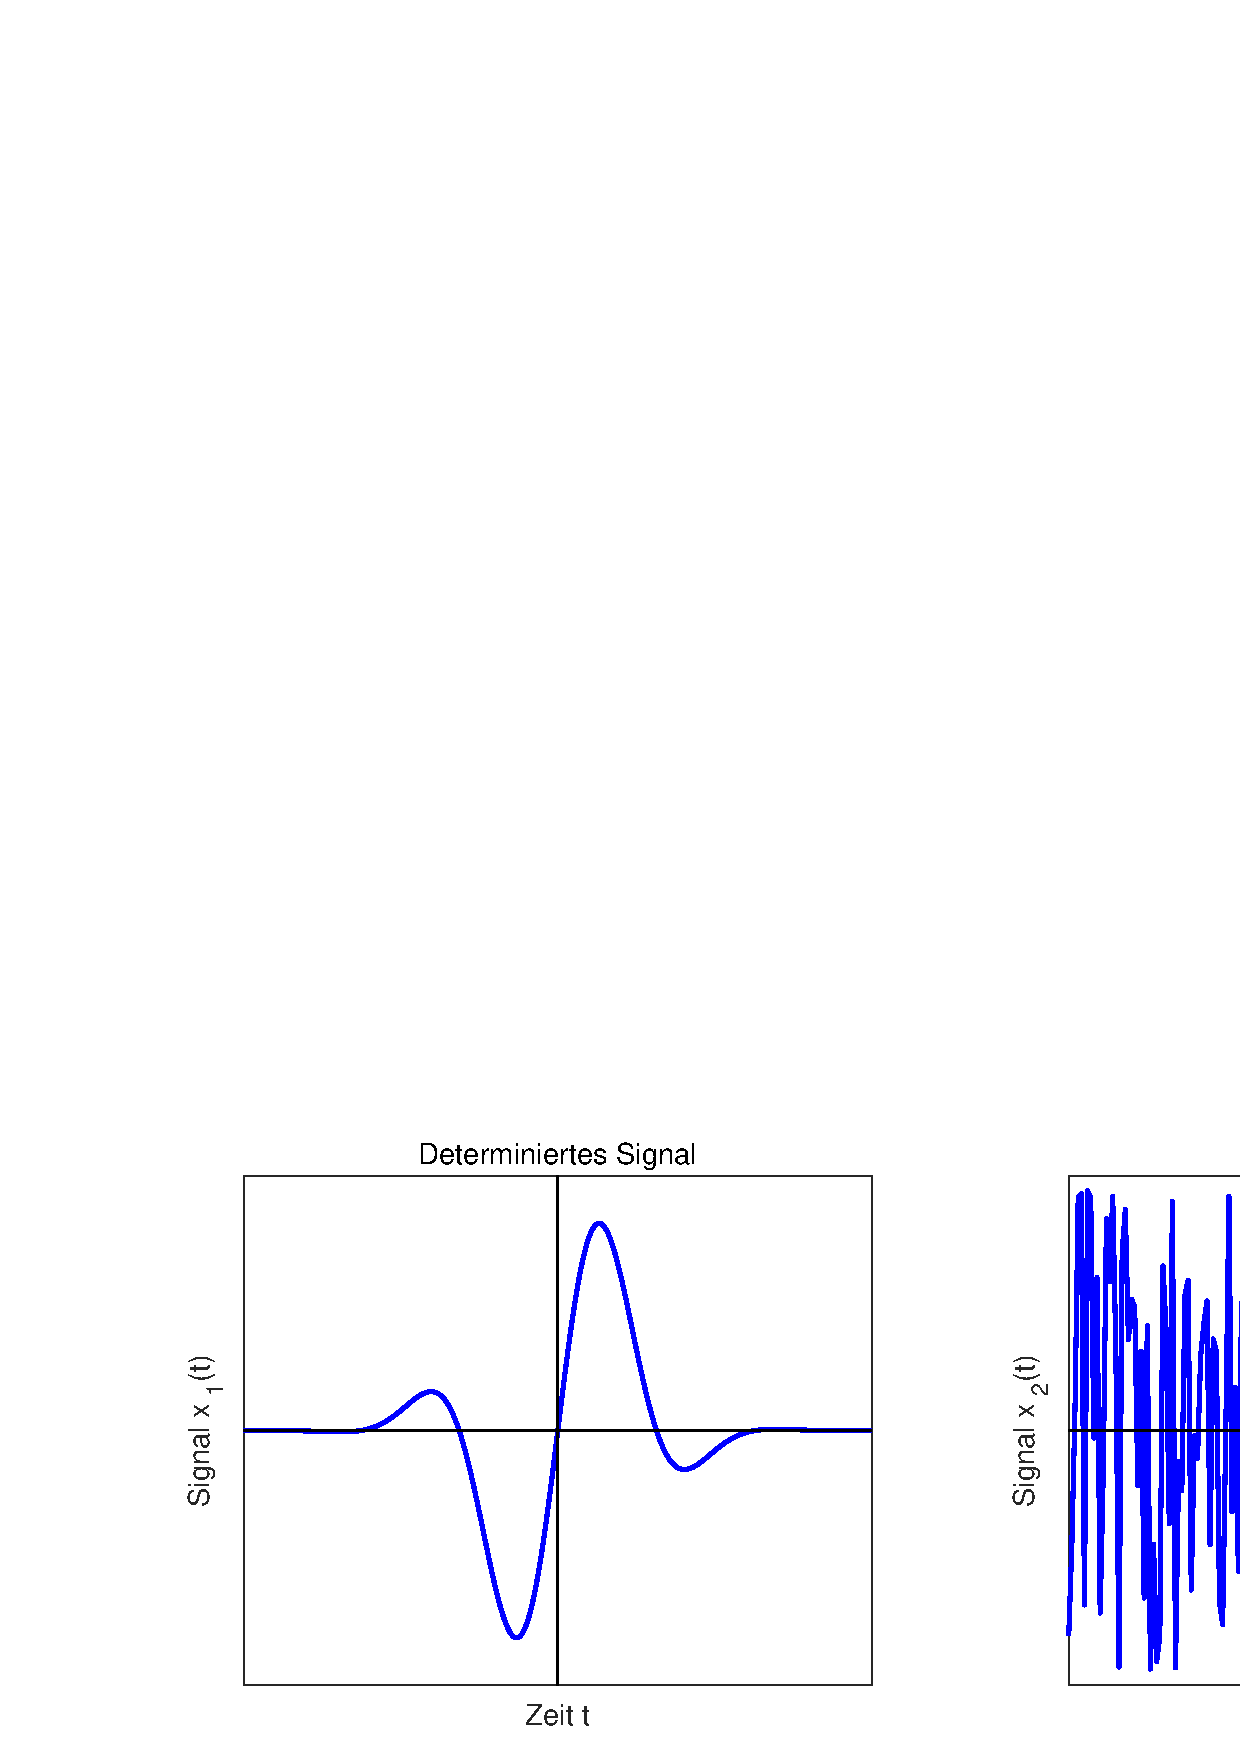
\includegraphics[width=0.1\textwidth]{Kapitel2/Table/image2.png}}} \\ \hline

\parbox[c][0.9in][c]{1.6in}{\centering{\fontfamily{phv}\selectfont{Sprungfunktion}}} &
\parbox[c][0.9in][c]{1.5in}{\centerline{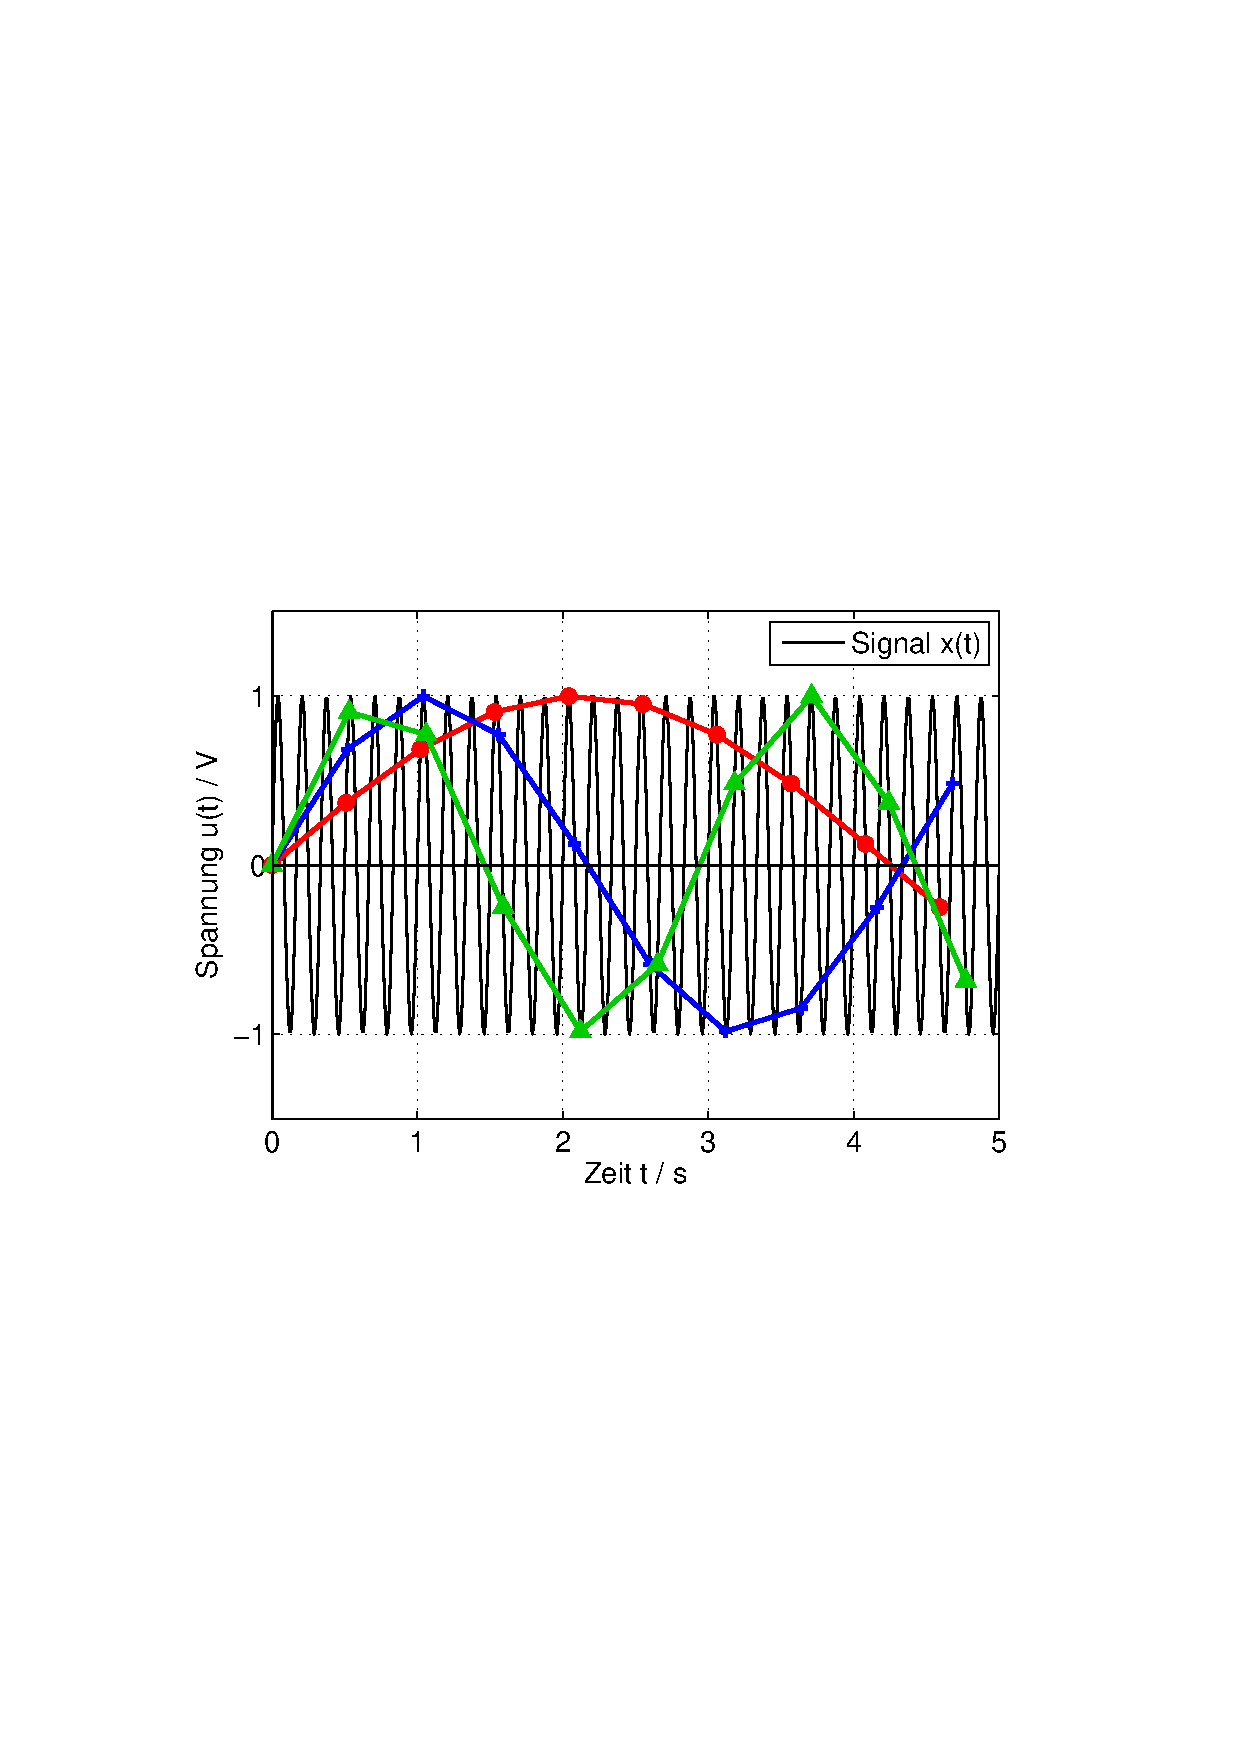
\includegraphics[width=0.085\textwidth]{Kapitel2/Table/image3.png}}}&
\parbox[c][0.9in][c]{1.6in}{\centering{\fontfamily{phv}\selectfont{Zugriff auf Variable im Workspace}}} &
\parbox[c][0.9in][c]{1.5in}{\centerline{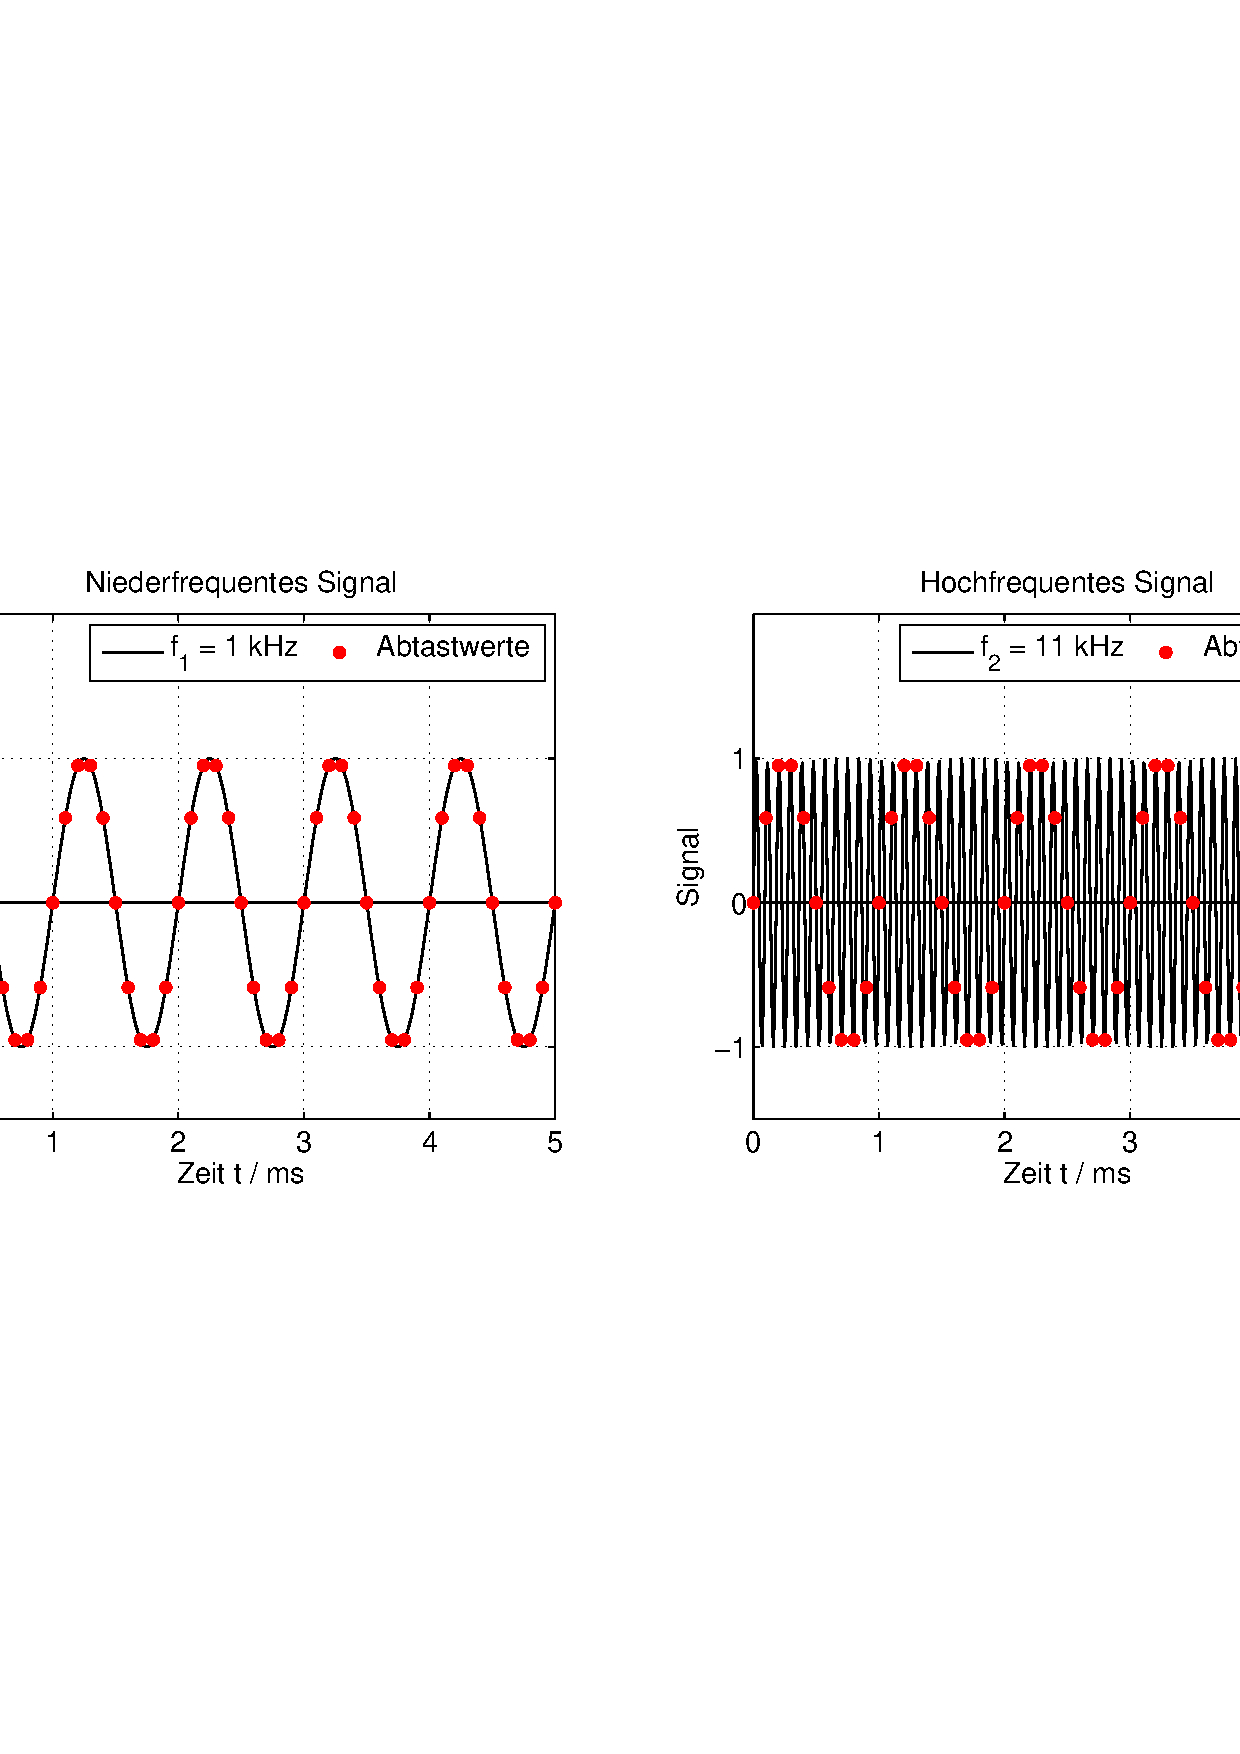
\includegraphics[width=0.12\textwidth]{Kapitel2/Table/image4.png}}} \\ \hline

\parbox[c][0.9in][c]{1.6in}{\centering{\fontfamily{phv}\selectfont{Rampenfunktion}}} &
\parbox[c][0.9in][c]{1.5in}{\centerline{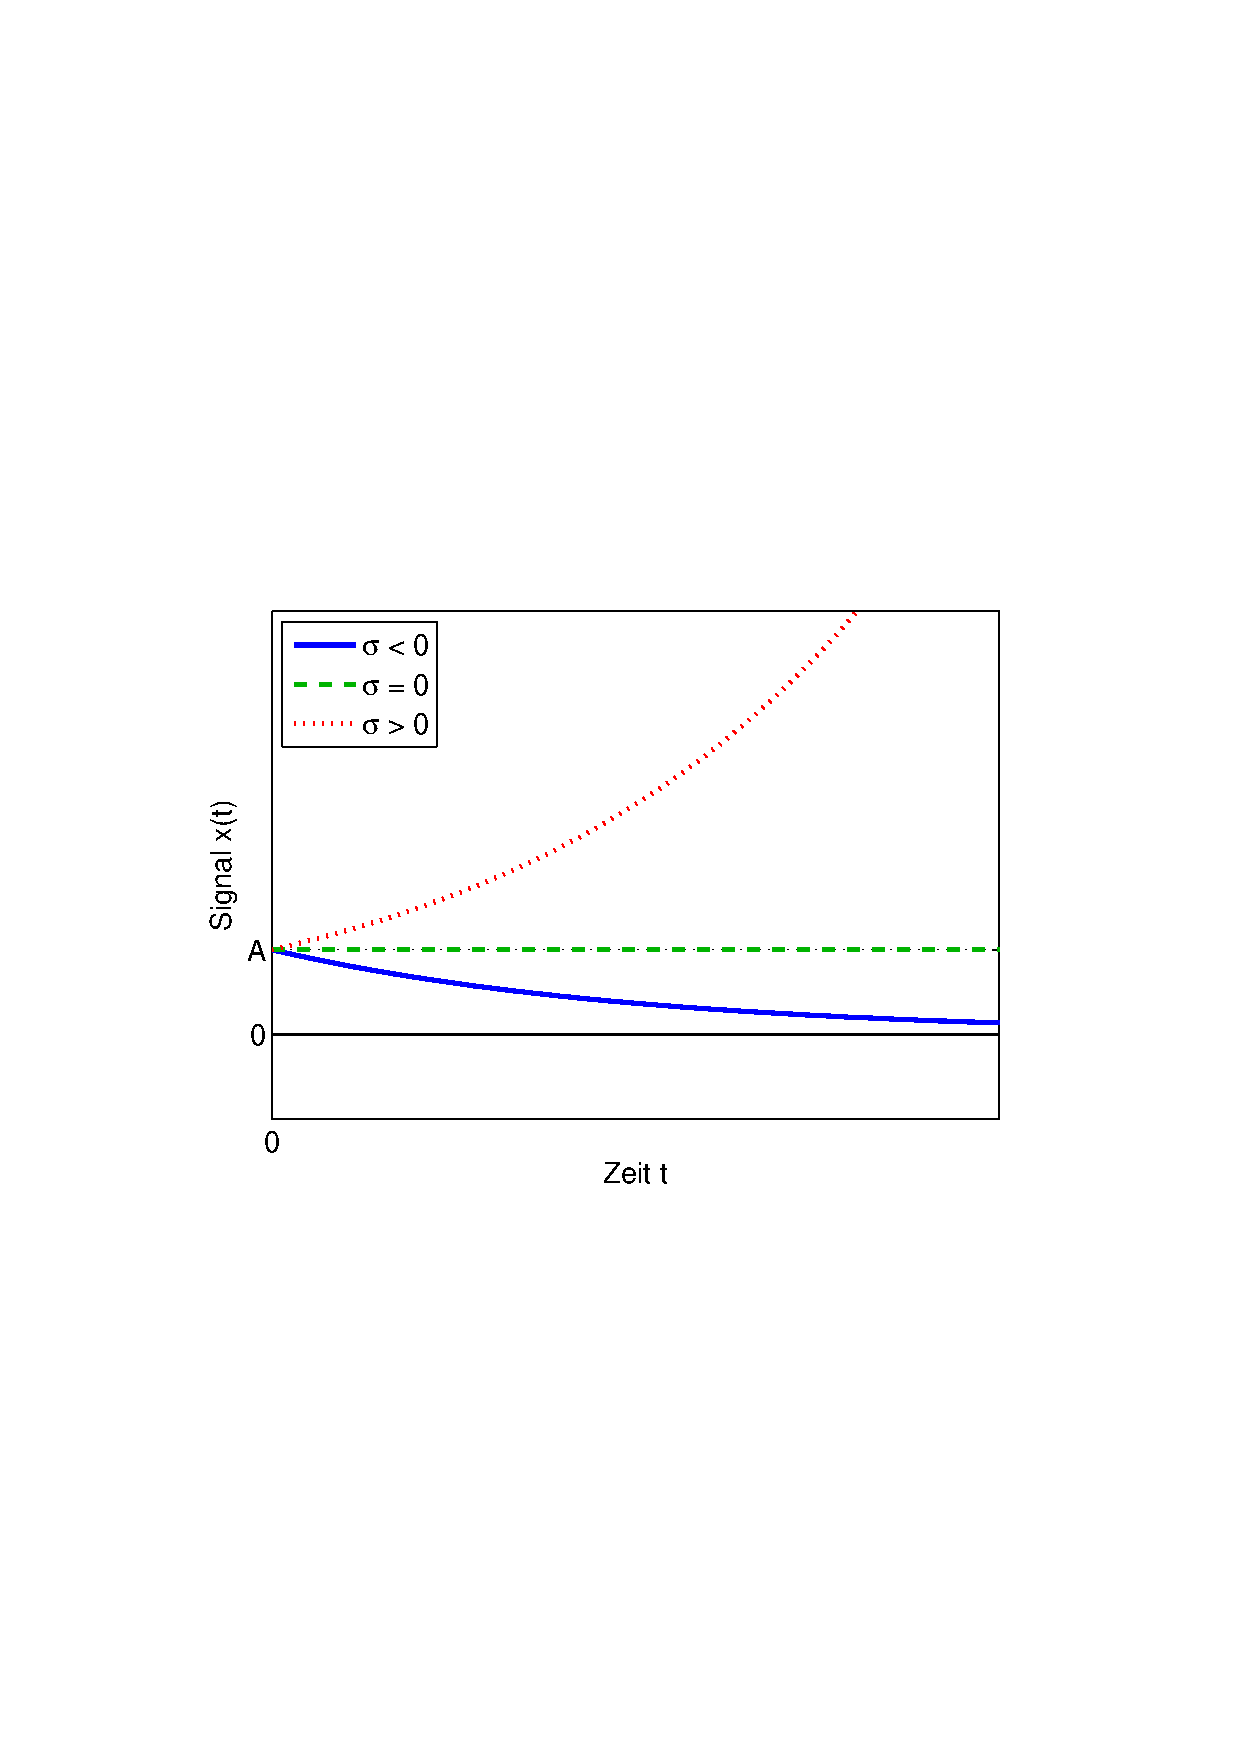
\includegraphics[width=0.085\textwidth]{Kapitel2/Table/image5.png}}} &
\parbox[c][0.9in][c]{1.6in}{\centering{\fontfamily{phv}\selectfont{Definition in mat-File}}} &
\parbox[c][0.9in][c]{1.5in}{\centerline{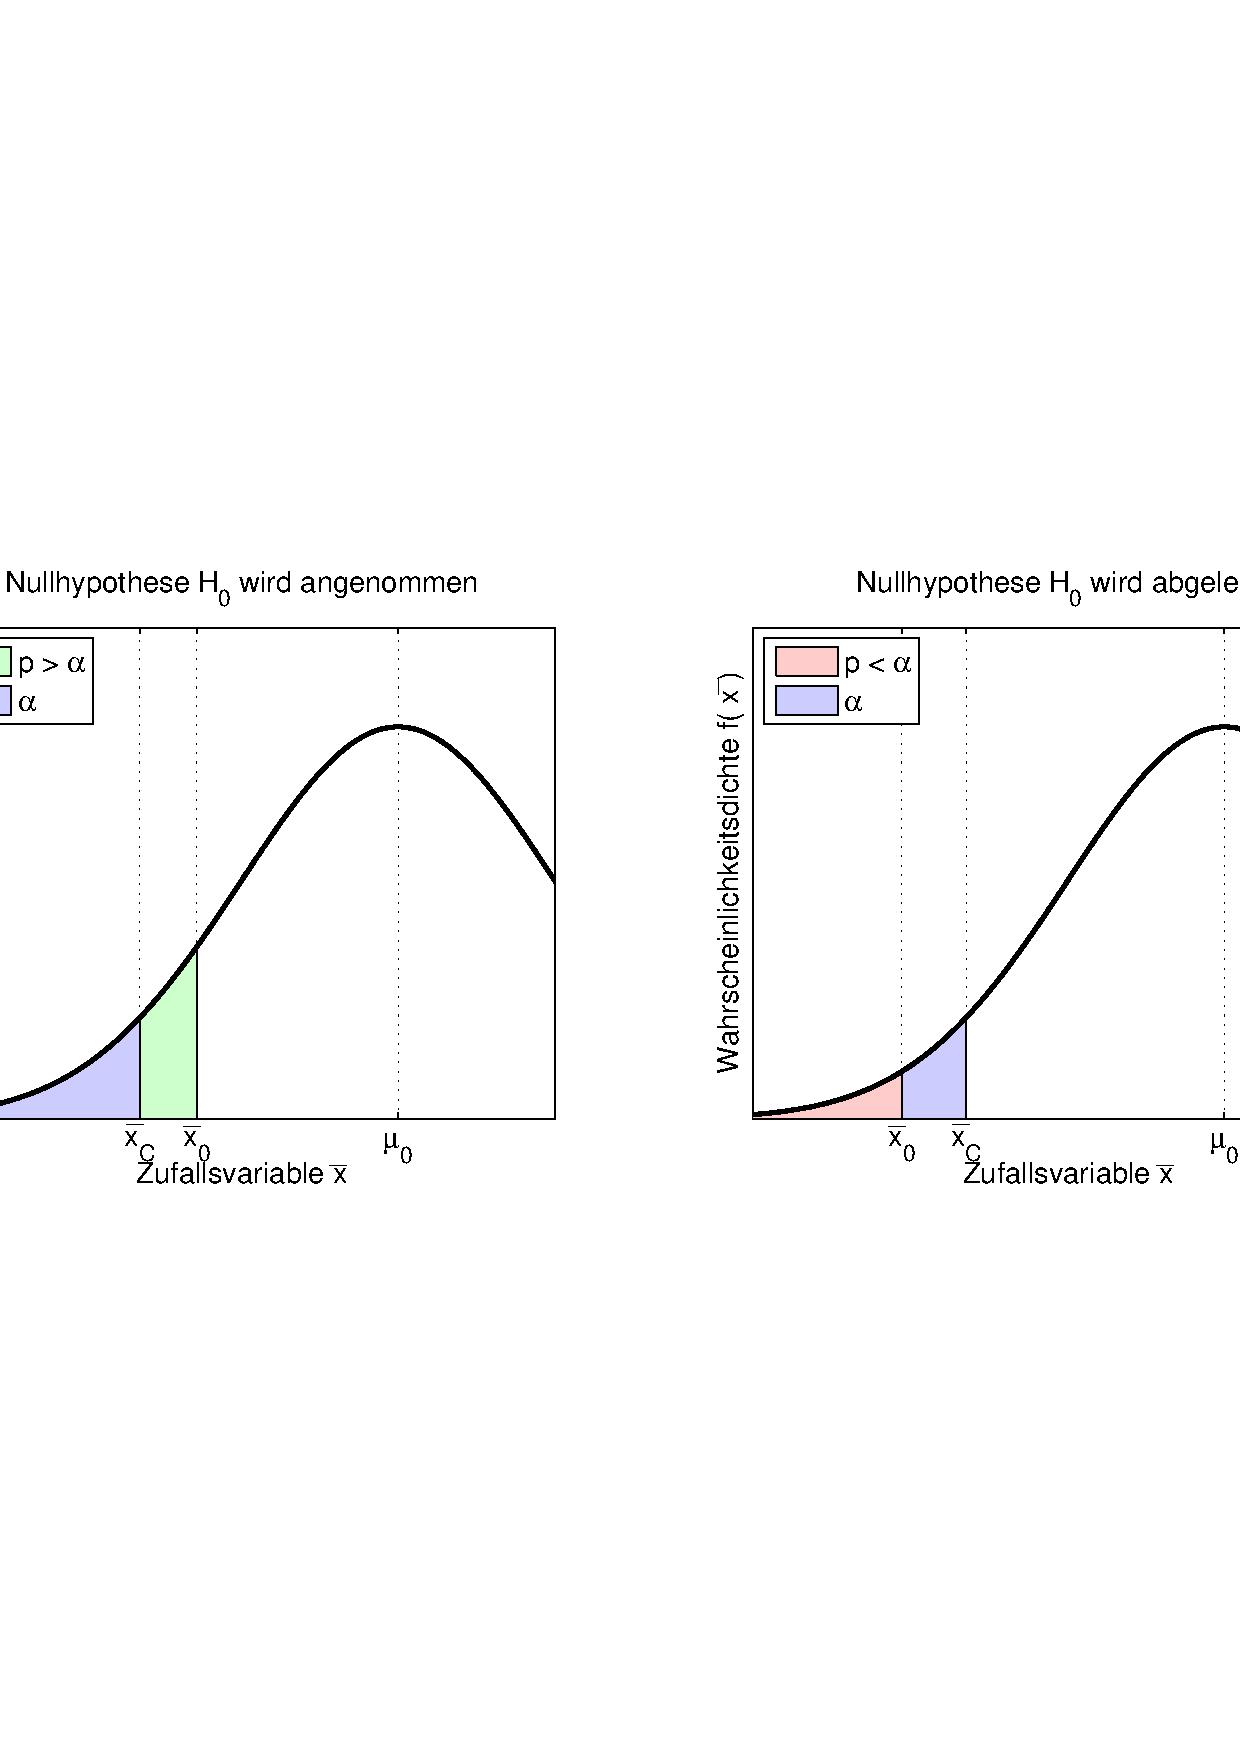
\includegraphics[width=0.12\textwidth]{Kapitel2/Table/image6.png}}} \\ \hline

\parbox[c][0.9in][c]{1.6in}{\centering{\fontfamily{phv}\selectfont{Rechteckfunktion}}} &
\parbox[c][0.9in][c]{1.5in}{\centerline{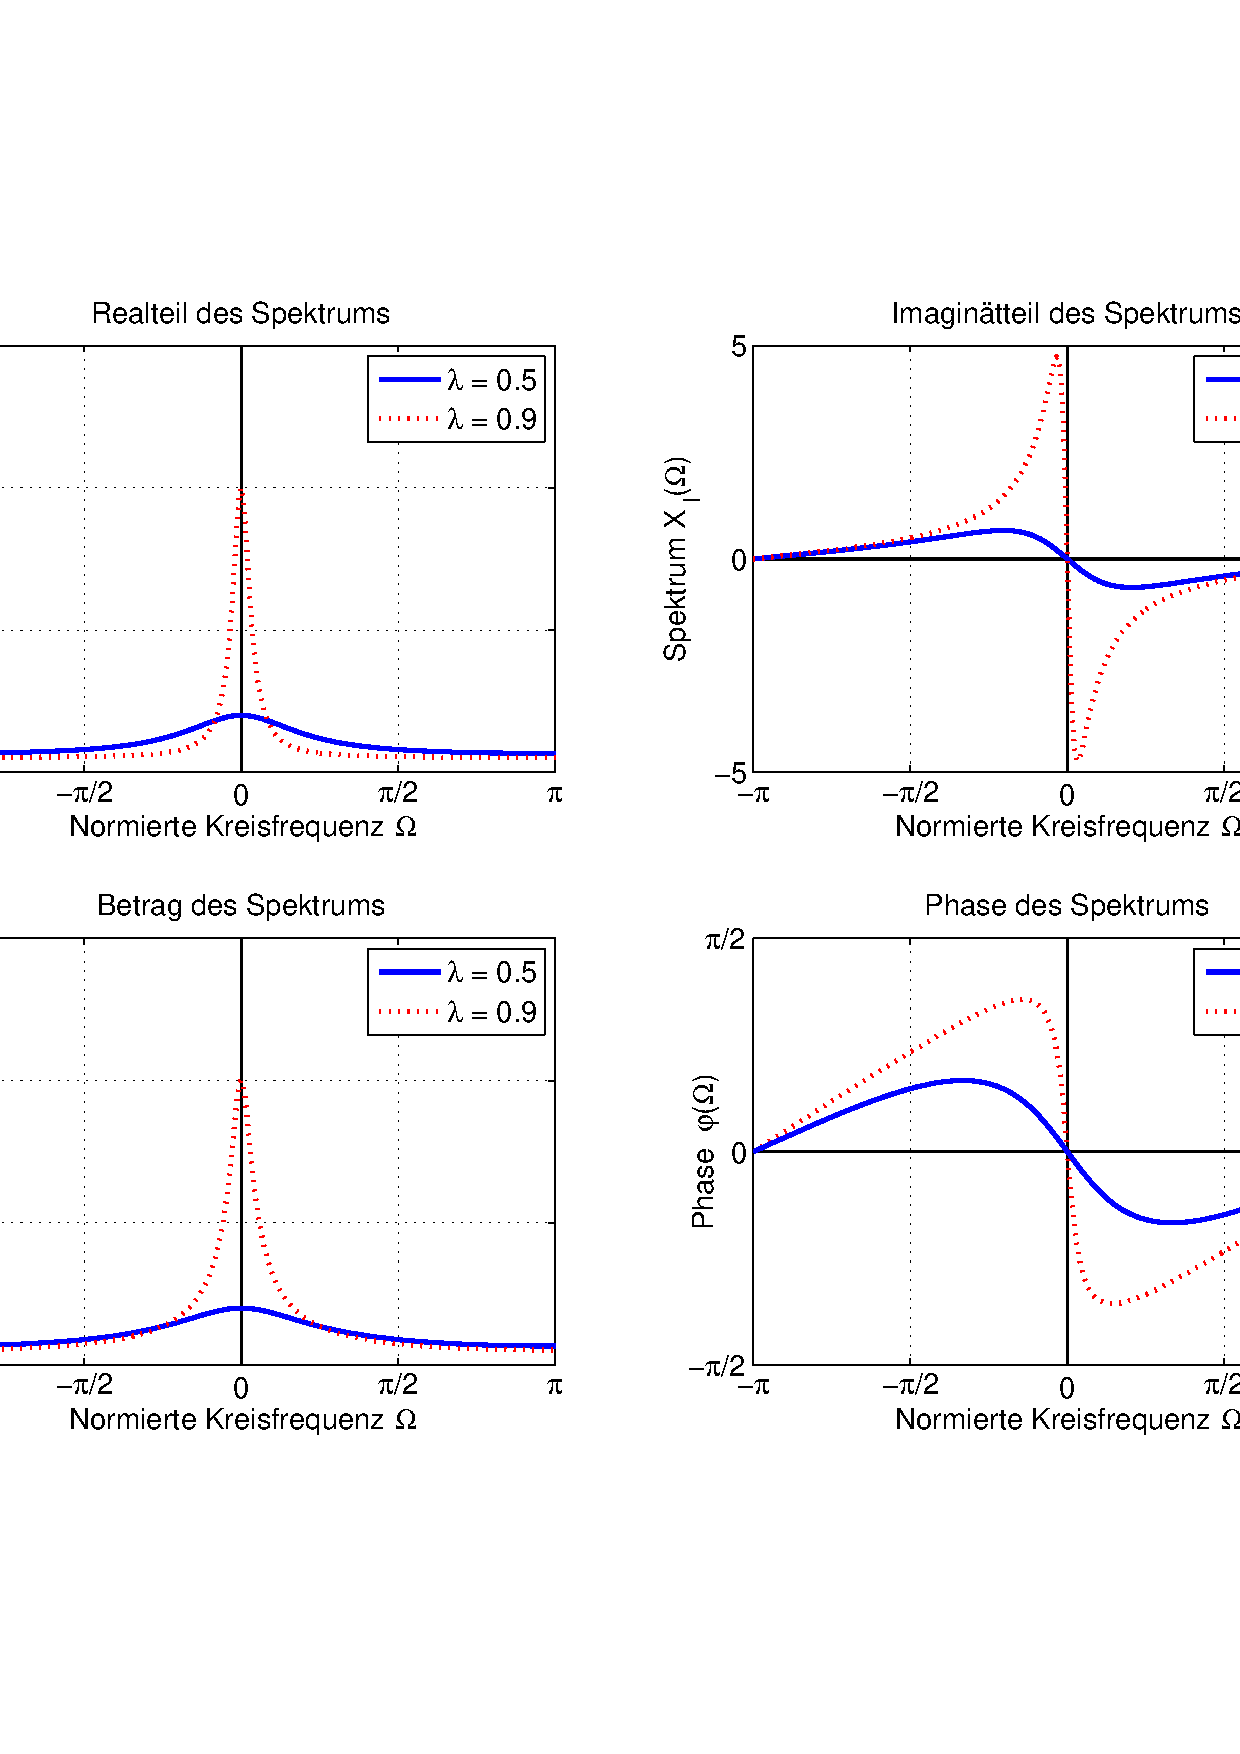
\includegraphics[width=0.1\textwidth]{Kapitel2/Table/image7.png}}} &
\parbox[c][0.9in][c]{1.6in}{\centering{\fontfamily{phv}\selectfont{Zeit}}} &
\parbox[c][0.9in][c]{1.5in}{\centerline{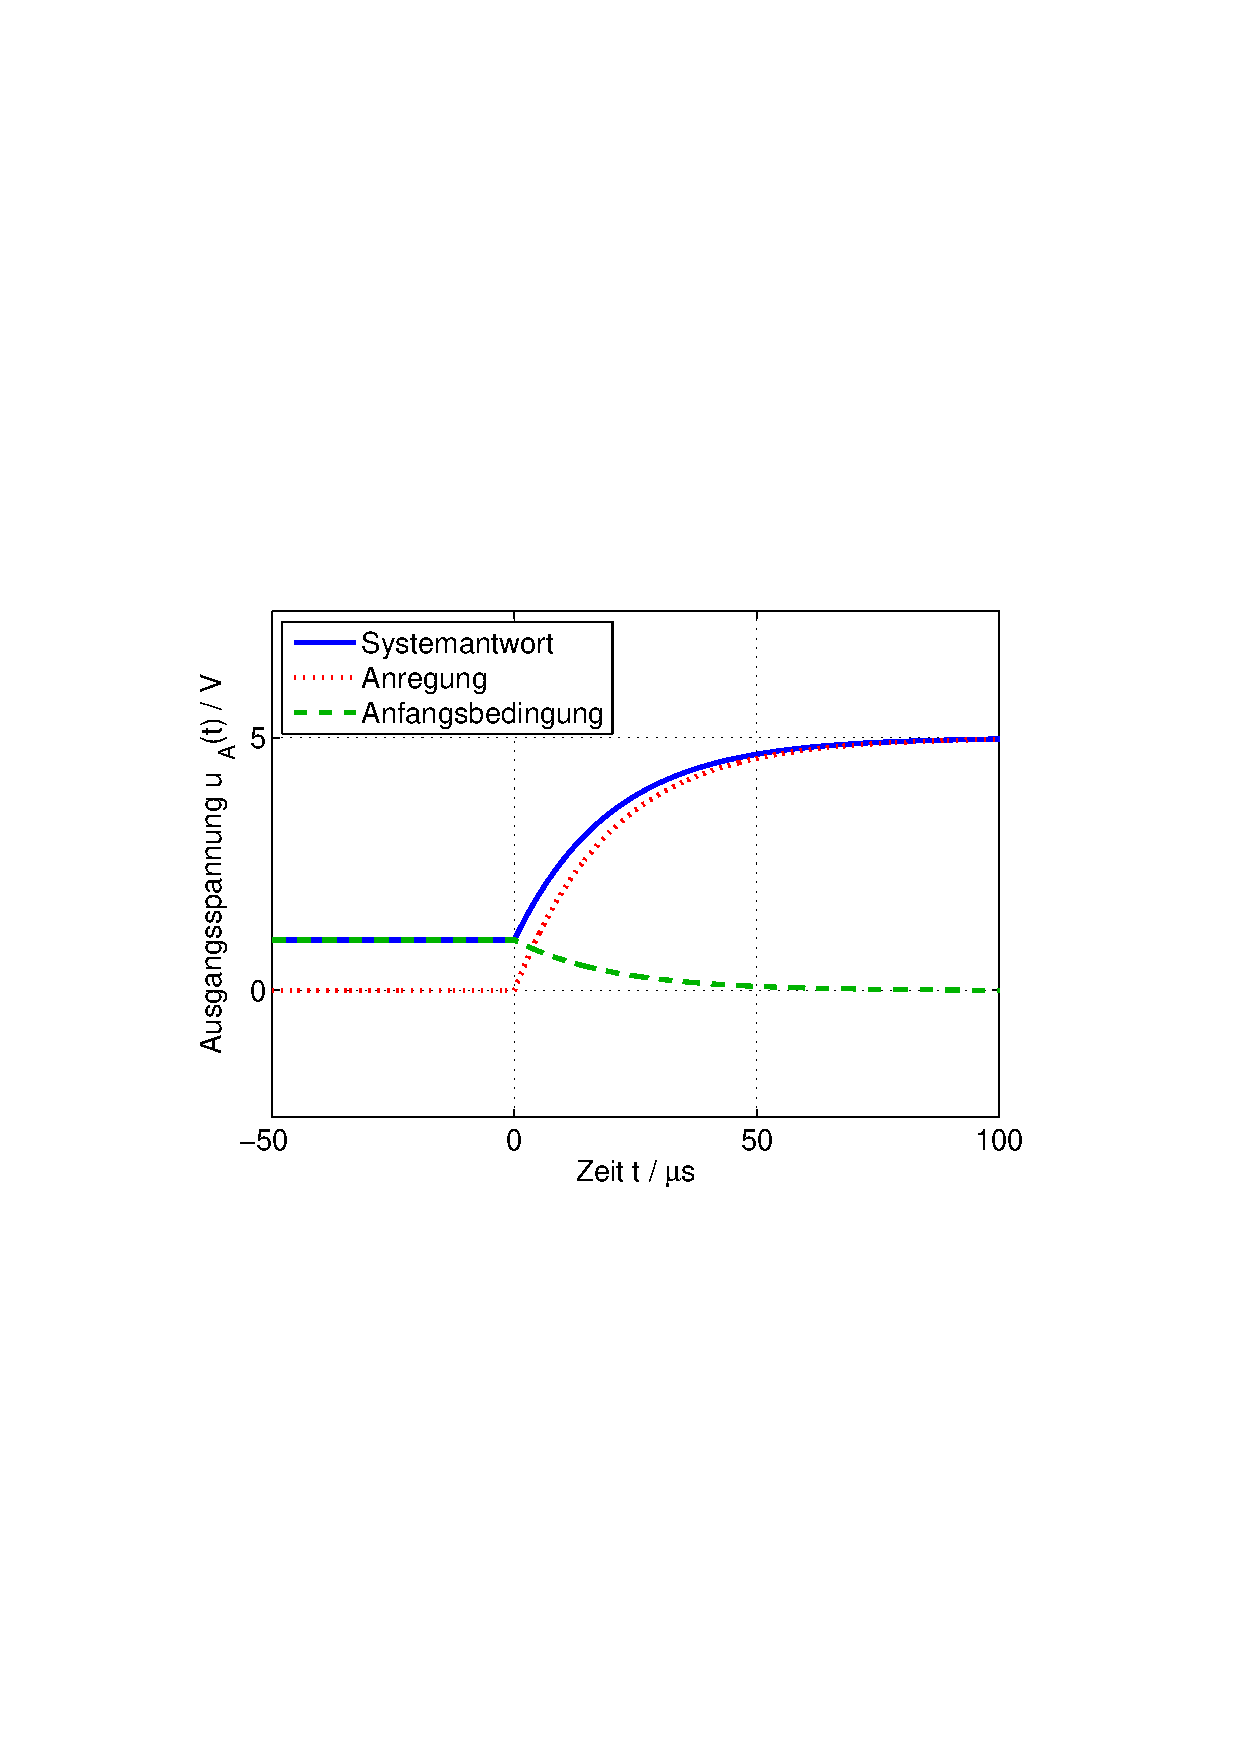
\includegraphics[width=0.07\textwidth]{Kapitel2/Table/image8.png}}}\\ \hline

\end{tabular}%
}\bigskip
\label{tab:threeeleven}
\end{table}

\medskip

{\fontfamily{phv}\selectfont
\noindent\textbf{Signalpfade und Verknüpfung von Signalpfaden}}

\noindent Simulink definiert Systeme über das Verbinden von Funktionsblöcken mit Signalpfaden. Zum Beispiel könnte ein System, das die Gleichung

\begin{equation}\label{eq:threetwohundredten}
y(t) = 3 \cdot u(t) + 1
\end{equation}

\noindent erfüllt, in Simulink über das Modell in Bild \ref{fig:SimulinkModell} dargestellt werden. Dabei wird u(t) als Signalquelle mit Sinusfunktion realisiert.

\begin{figure}[H]
  \centerline{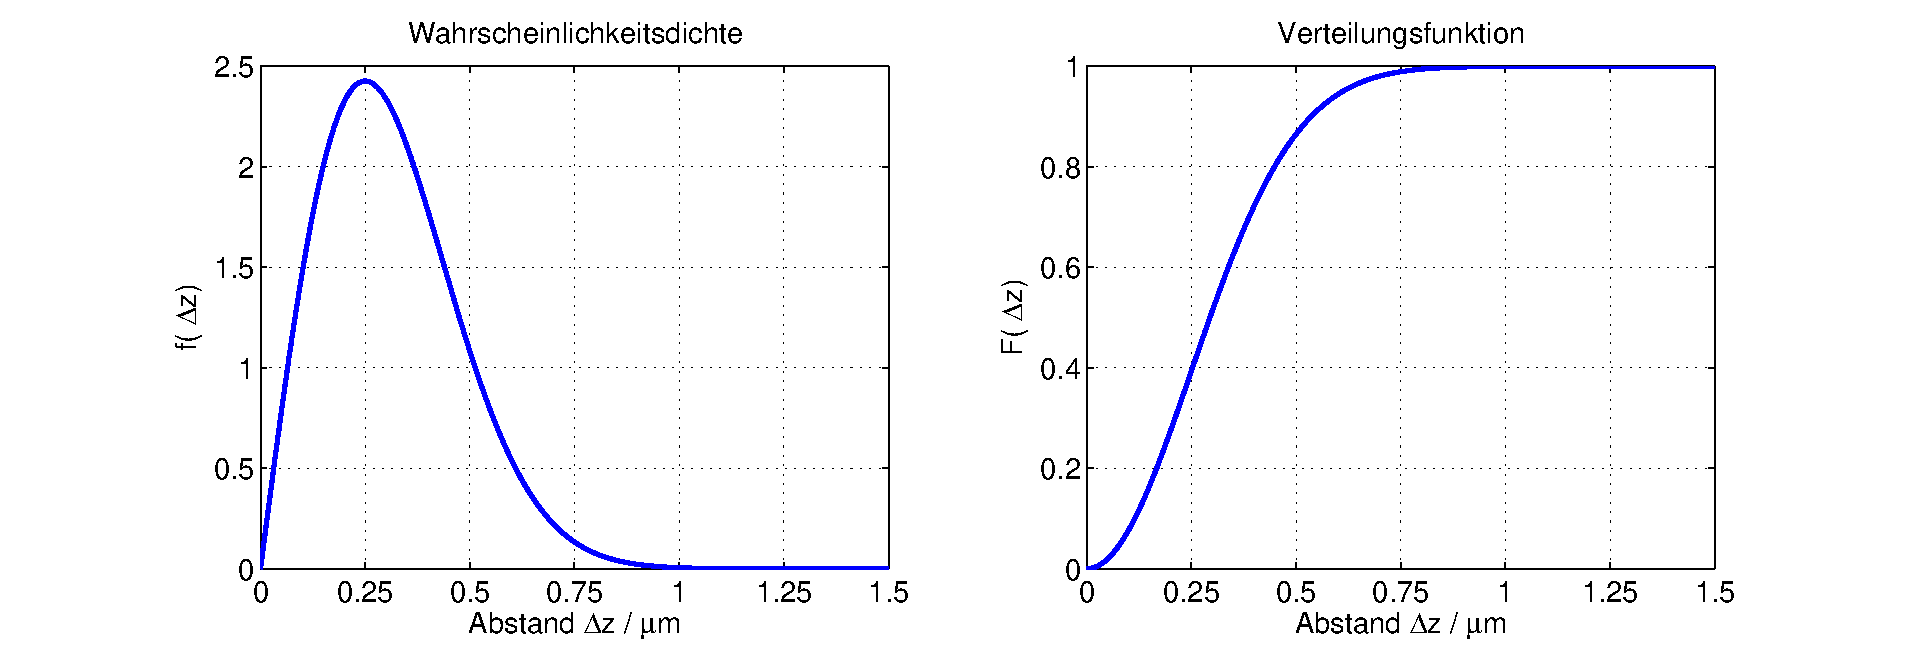
\includegraphics[width=0.5\textwidth]{Kapitel2/Bilder/image33}}
  \caption{Einfaches Simulink Modell}
  \label{fig:SimulinkModell}
\end{figure}

\noindent Die Signalpfade laufen durch Blöcke, die eine definierte Funktion ausführen. Diese Funktion kann neben Additionen, Subtraktion, Multiplikation und Division auch eine höhere mathematische Funktion sein, die als \textit{Math-Function-Block} definiert wird. Mit den Blöcken Multiplexer und Demultiplexer können Signale zu einem mehrdimensionalen Signalpfad zusammengefasst beziehungsweise von einem Signalpfad in einzelne Signale zerlegt werden. Tabelle \ref{tab:threetwelve} stellt eine Auswahl von Verknüpfungen in Simulink dar.

\clearpage
\begin{table}[H]
\caption{Auswahl von Funktionen zur Signalverknüpfung}
\setlength{\fboxsep}{0pt}%
\colorbox{lightgray}{%
\arrayrulecolor{white}%
\begin{tabular}{| c | c | c | c |}
\hline
\parbox[c][0.28in][c]{1.6in}{\smallskip\centering\textbf{\fontfamily{phv}\selectfont{Operation}}} & \parbox[c][0.28in][c]{1.5in}{\smallskip\centering\textbf{\fontfamily{phv}\selectfont{Simulink Symbol}}} &
\parbox[c][0.28in][c]{1.6in}{\smallskip\centering\textbf{\fontfamily{phv}\selectfont{Operation}}} &
\parbox[c][0.28in][c]{1.5in}{\smallskip\centering\textbf{\fontfamily{phv}\selectfont{Simulink Symbol}}}\\ \hline


\parbox[c][0.9in][c]{1.6in}{\centering{\fontfamily{phv}\selectfont{Addition von Signalen}}} &
\parbox[c][0.9in][c]{1.5in}{\centerline{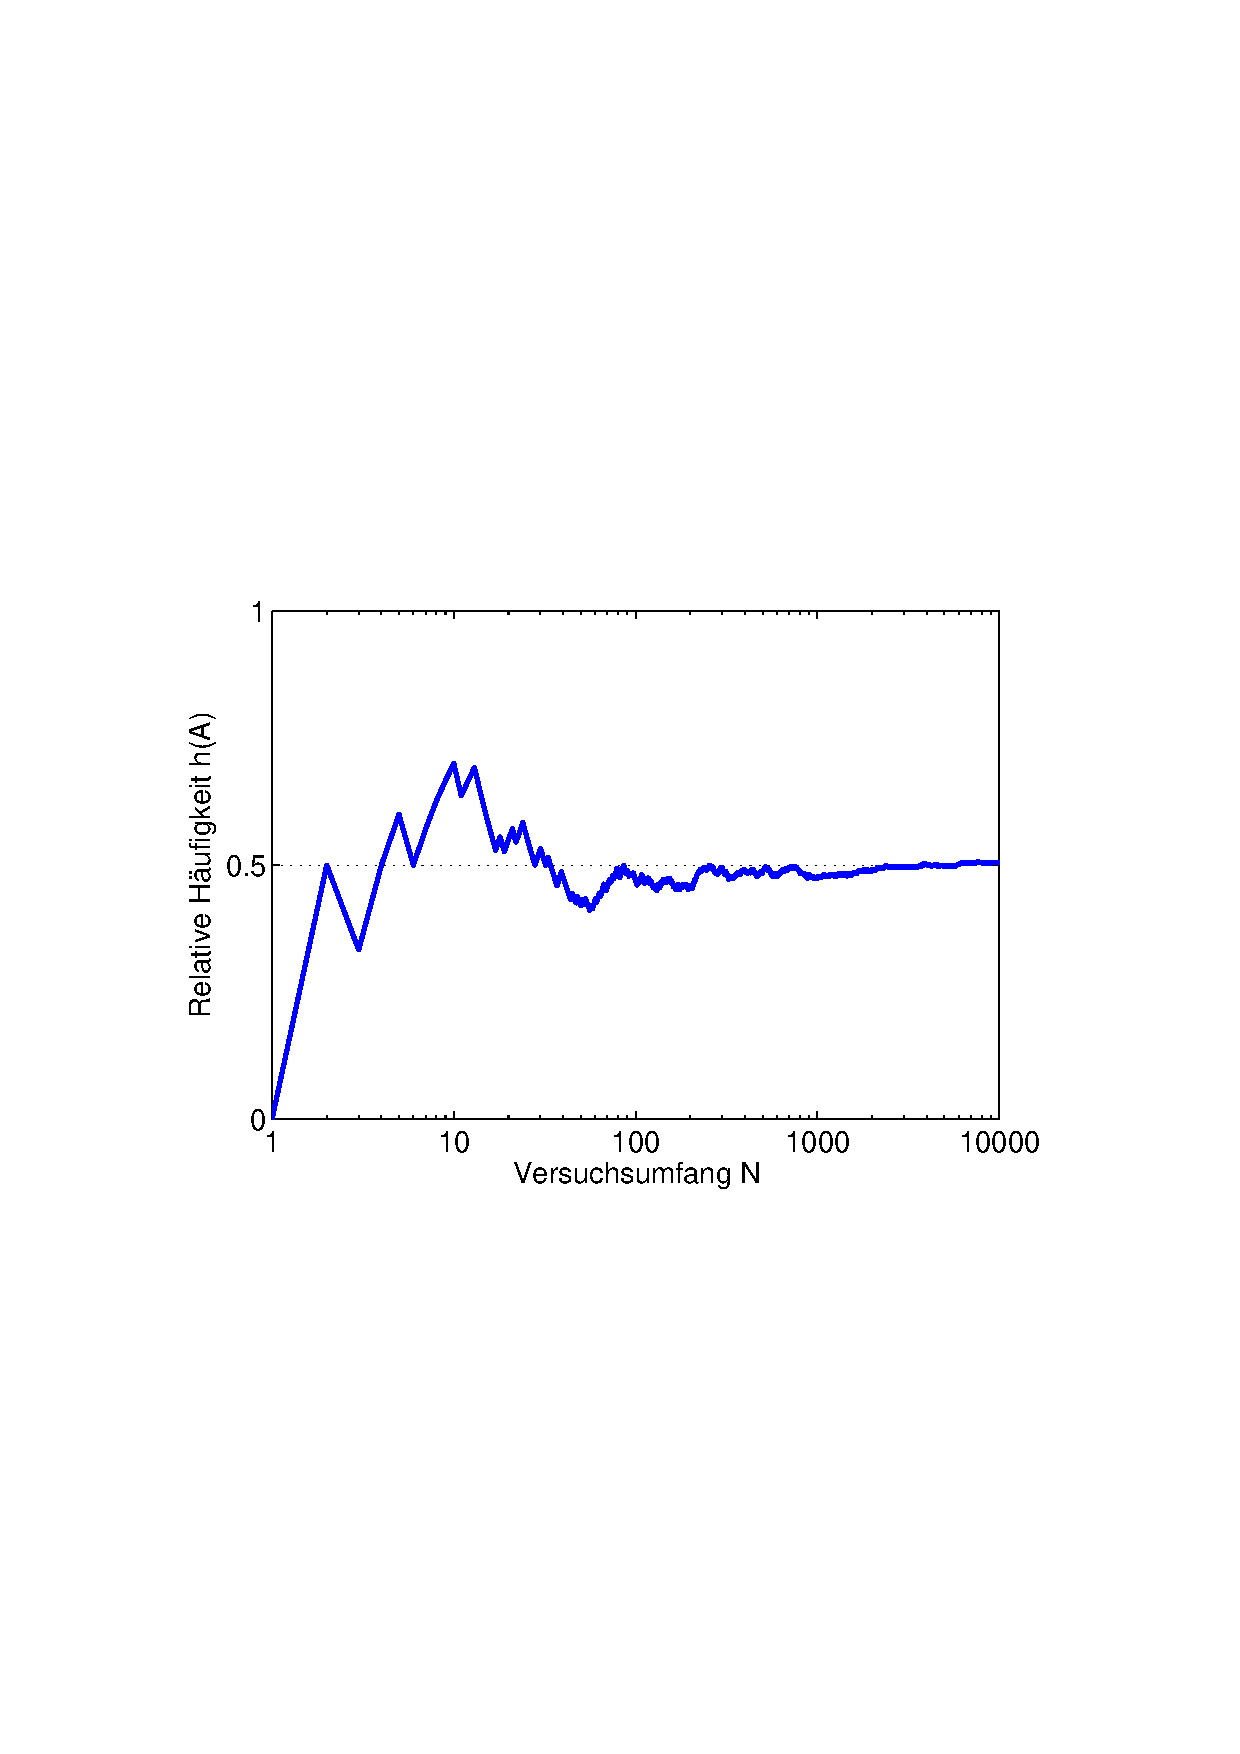
\includegraphics[width=0.1\textwidth]{Kapitel2/Table/image9.png}}} &
\parbox[c][0.9in][c]{1.6in}{\centering{\fontfamily{phv}\selectfont{Multiplikation / Division \\ von Signalen}}} &
\parbox[c][0.9in][c]{1.5in}{\centerline{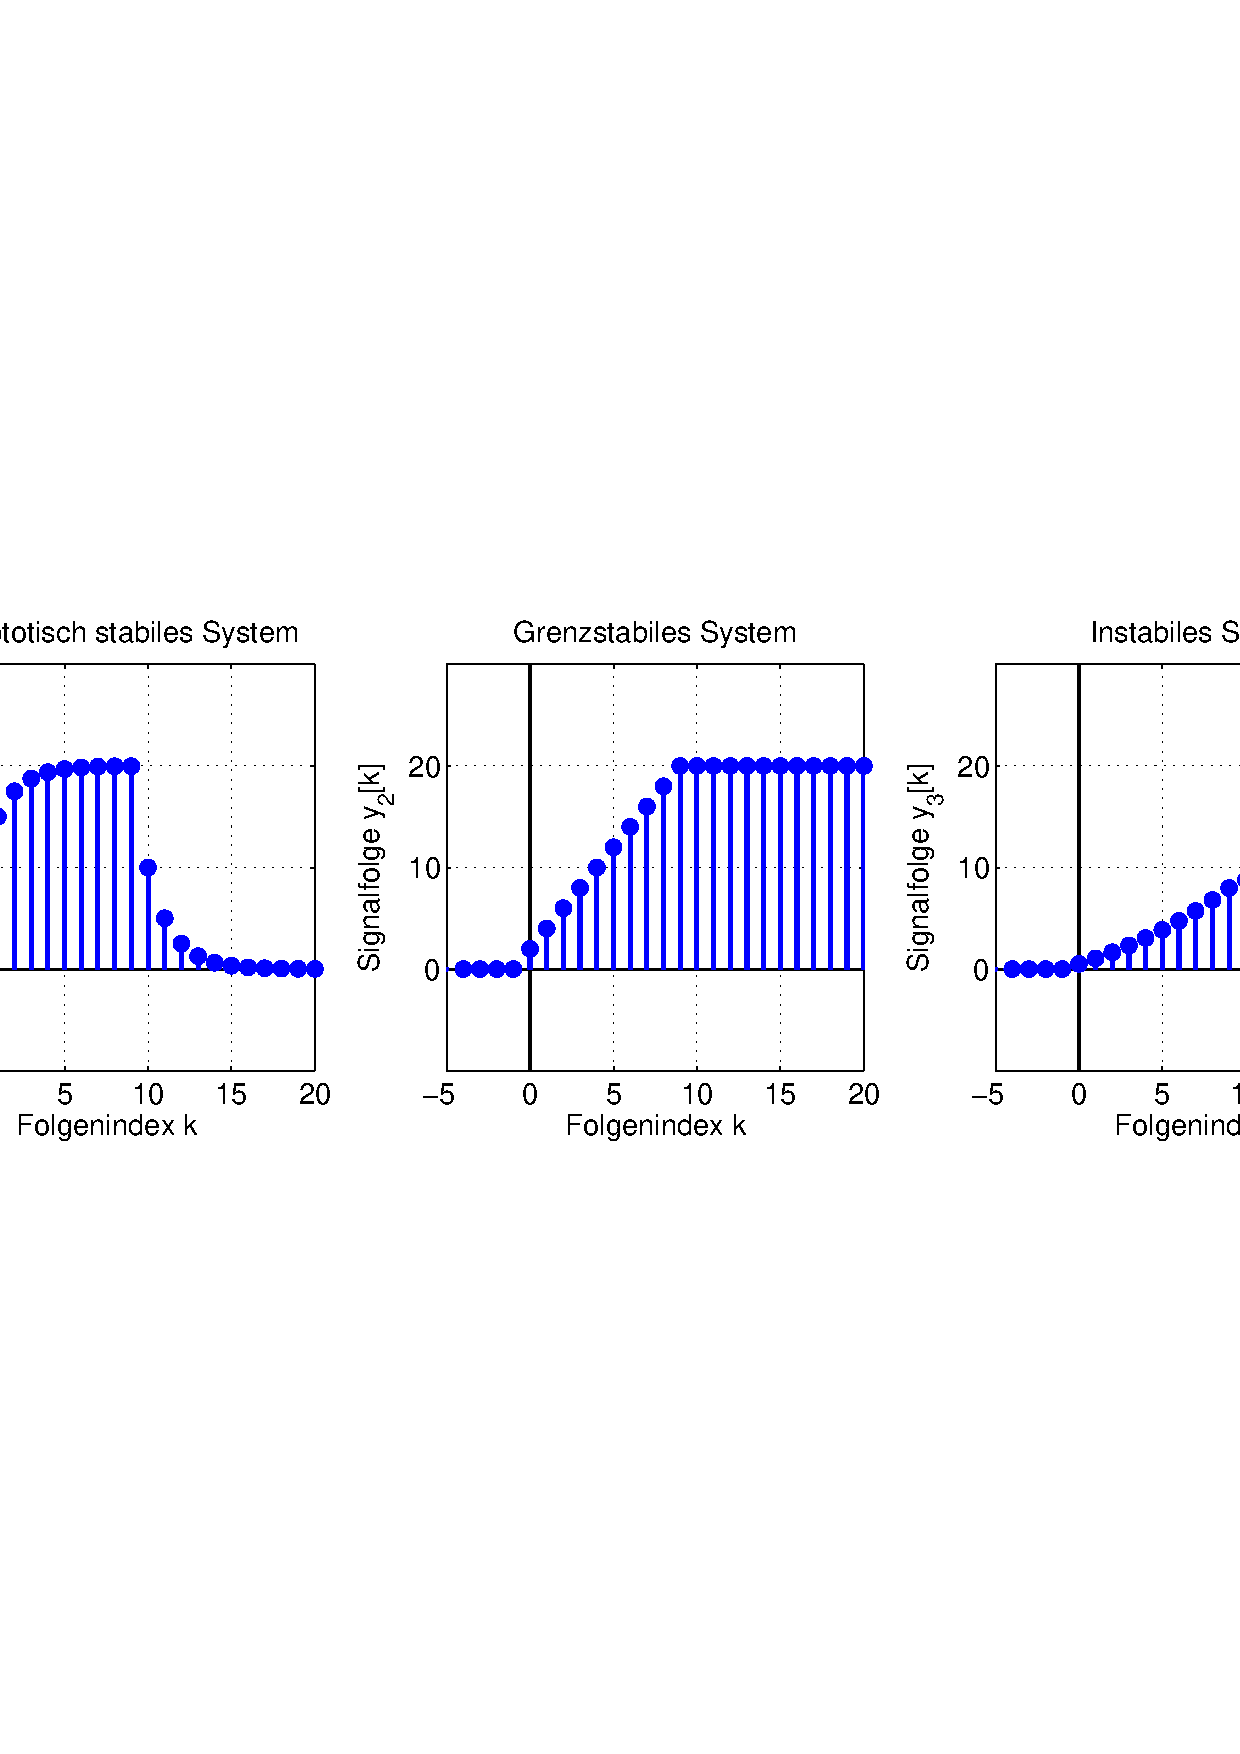
\includegraphics[width=0.1\textwidth]{Kapitel2/Table/image10.png}}} \\ \hline

\parbox[c][0.9in][c]{1.6in}{\centering{\fontfamily{phv}\selectfont{Multiplikation \\
mit einem Faktor, \\
Verstärkung}}} &
\parbox[c][0.9in][c]{1.5in}{\centerline{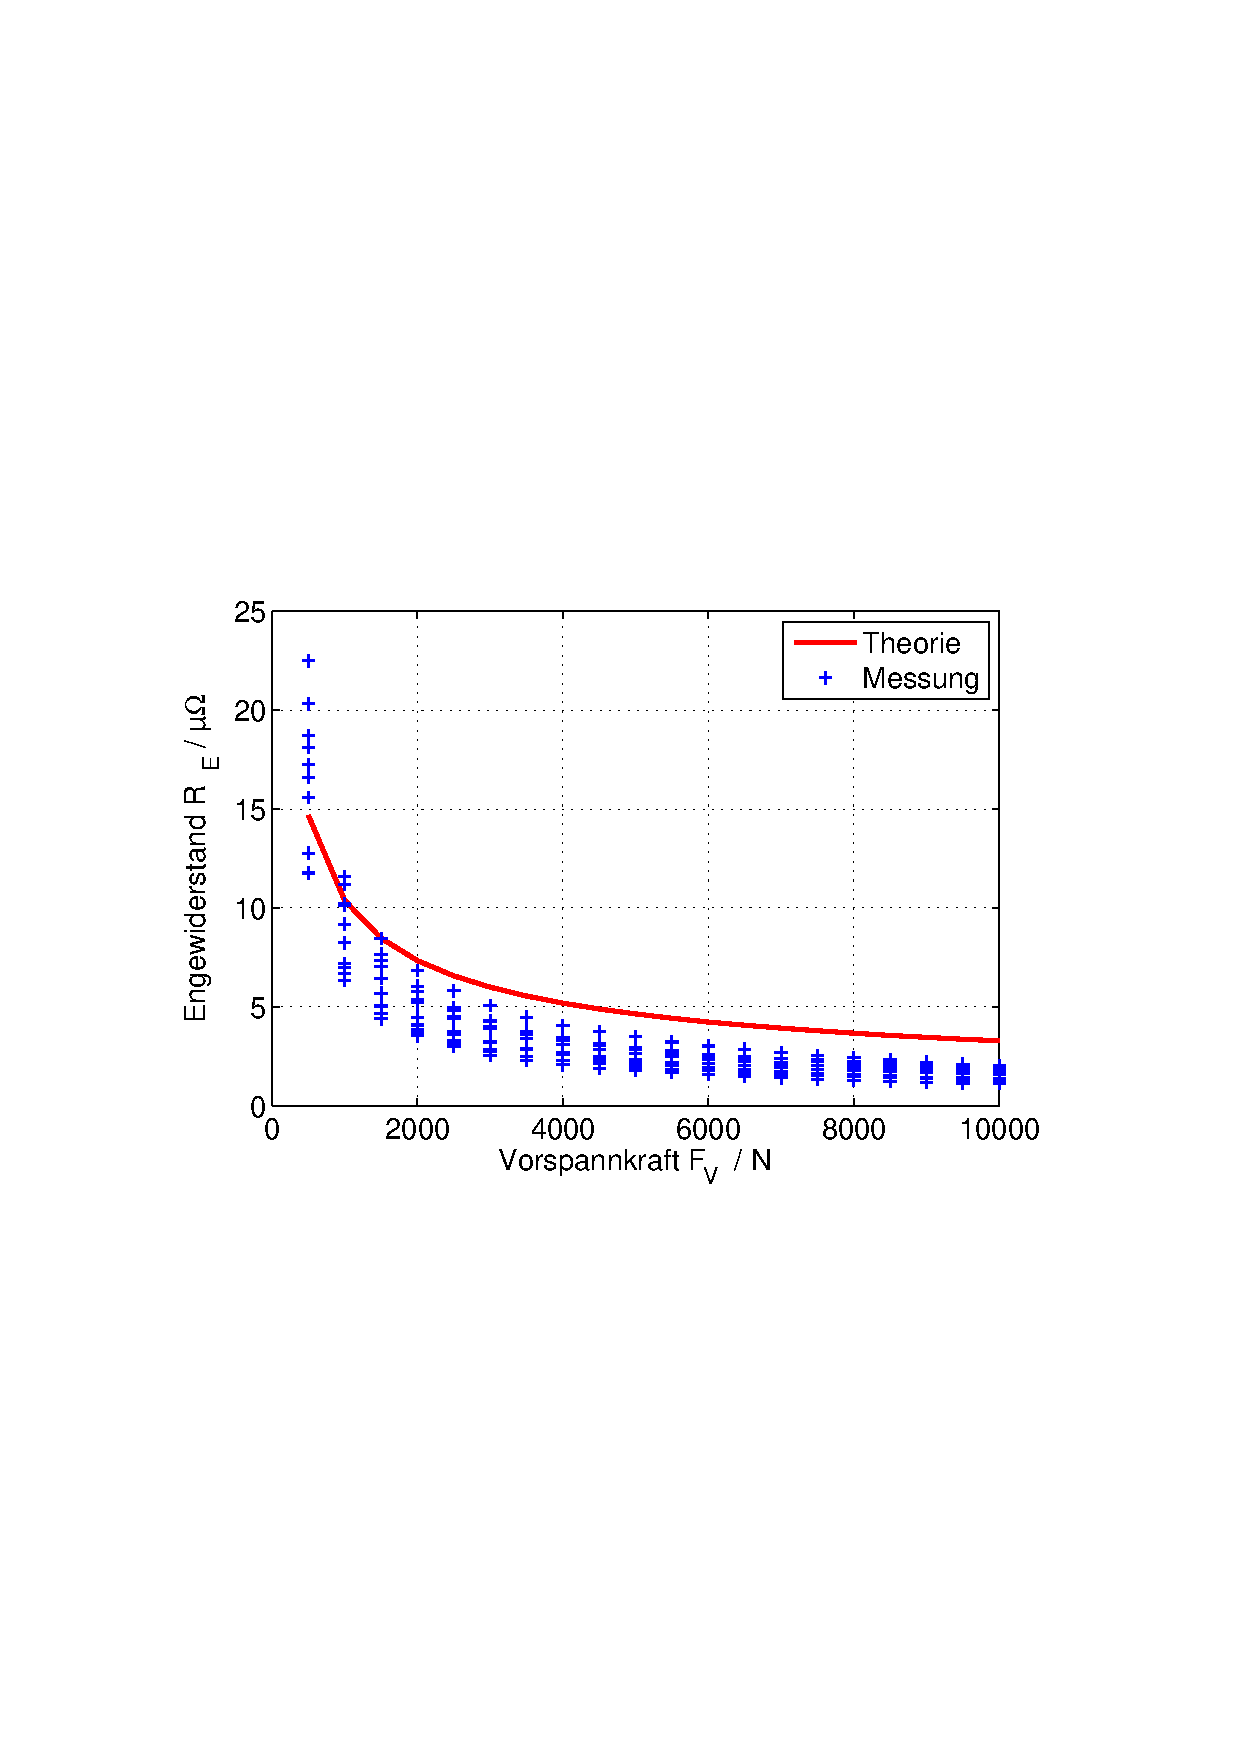
\includegraphics[width=0.1\textwidth]{Kapitel2/Table/image11.png}}} &
\parbox[c][0.9in][c]{1.6in}{\centering{\fontfamily{phv}\selectfont{Mathematische \\
Funktionen}}} &
\parbox[c][0.9in][c]{1.5in}{\centerline{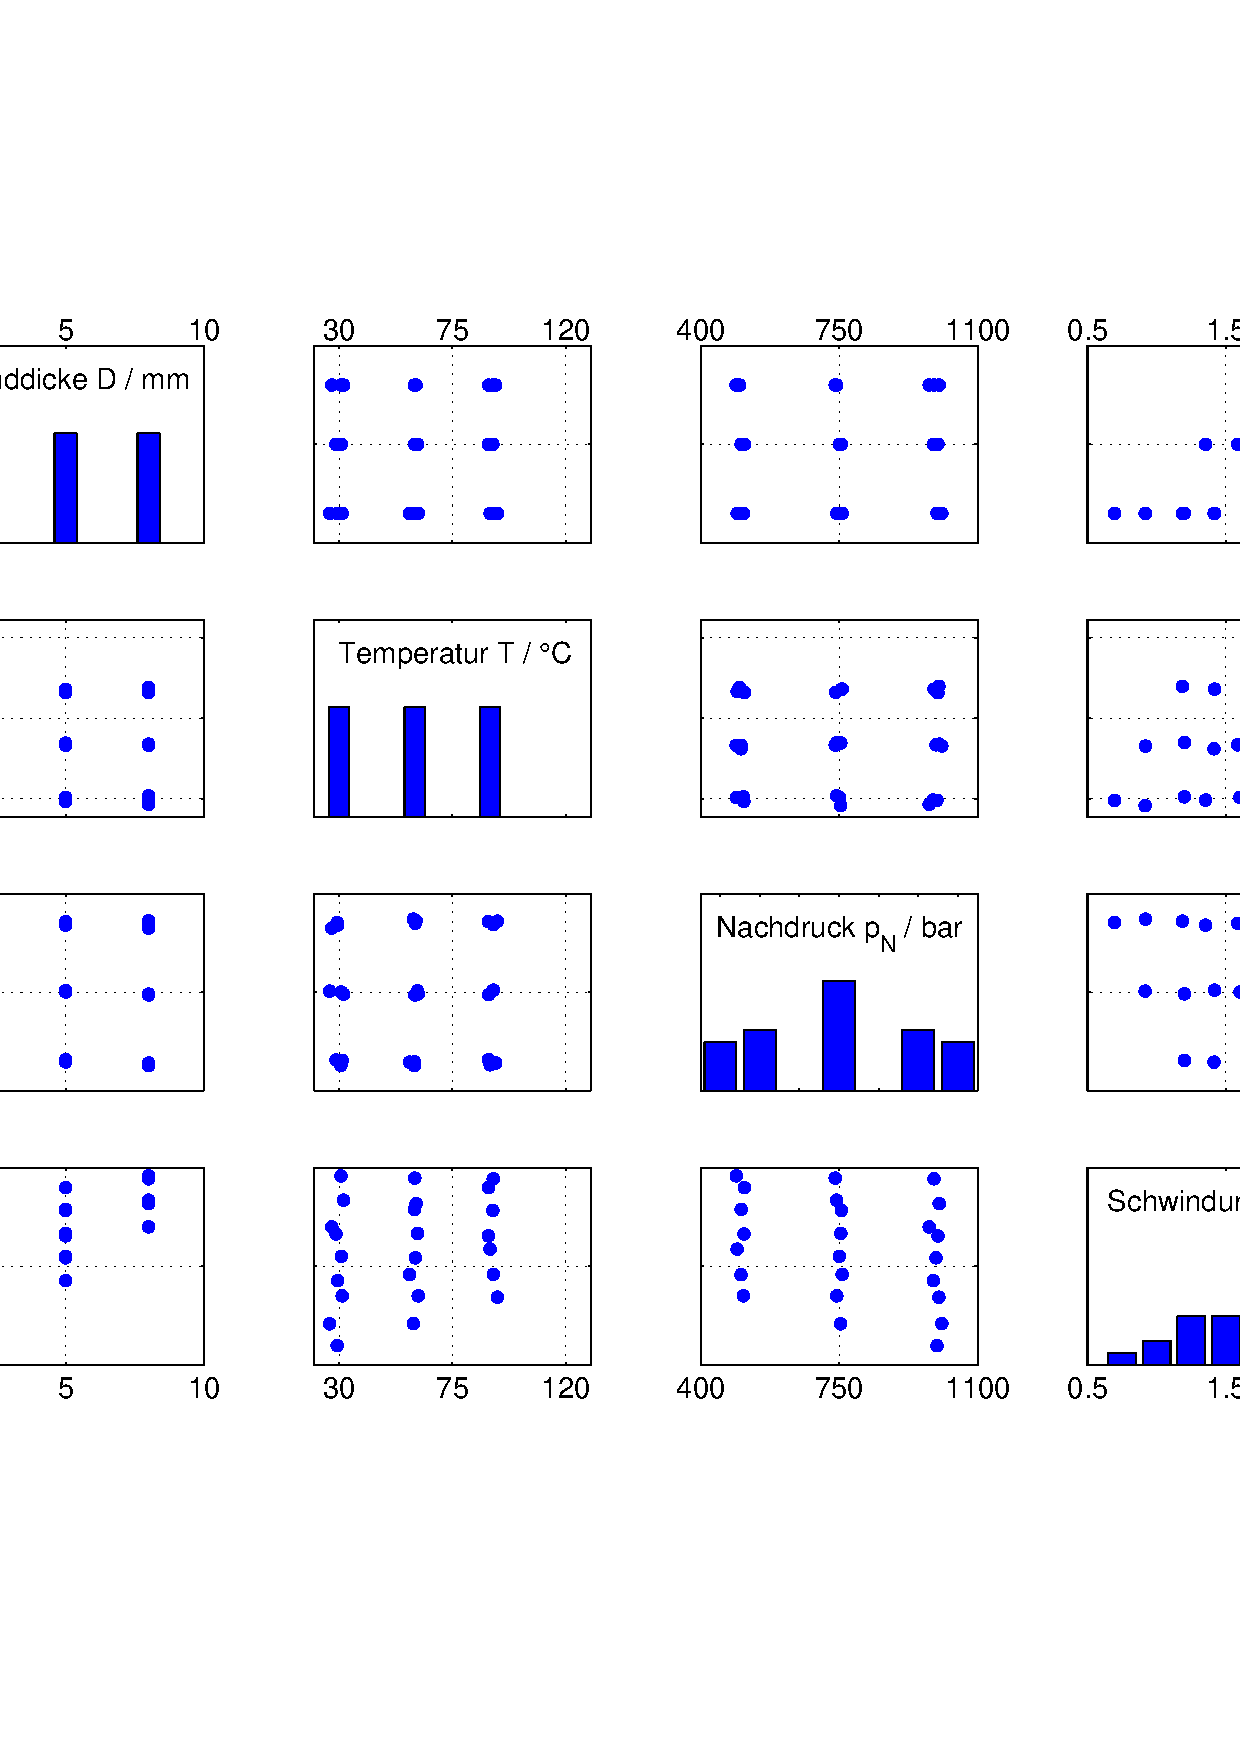
\includegraphics[width=0.1\textwidth]{Kapitel2/Table/image12.png}}} \\ \hline

\parbox[c][0.9in][c]{1.6in}{\centering{\fontfamily{phv}\selectfont{Multiplexer}}} &
\parbox[c][0.9in][c]{1.5in}{\centerline{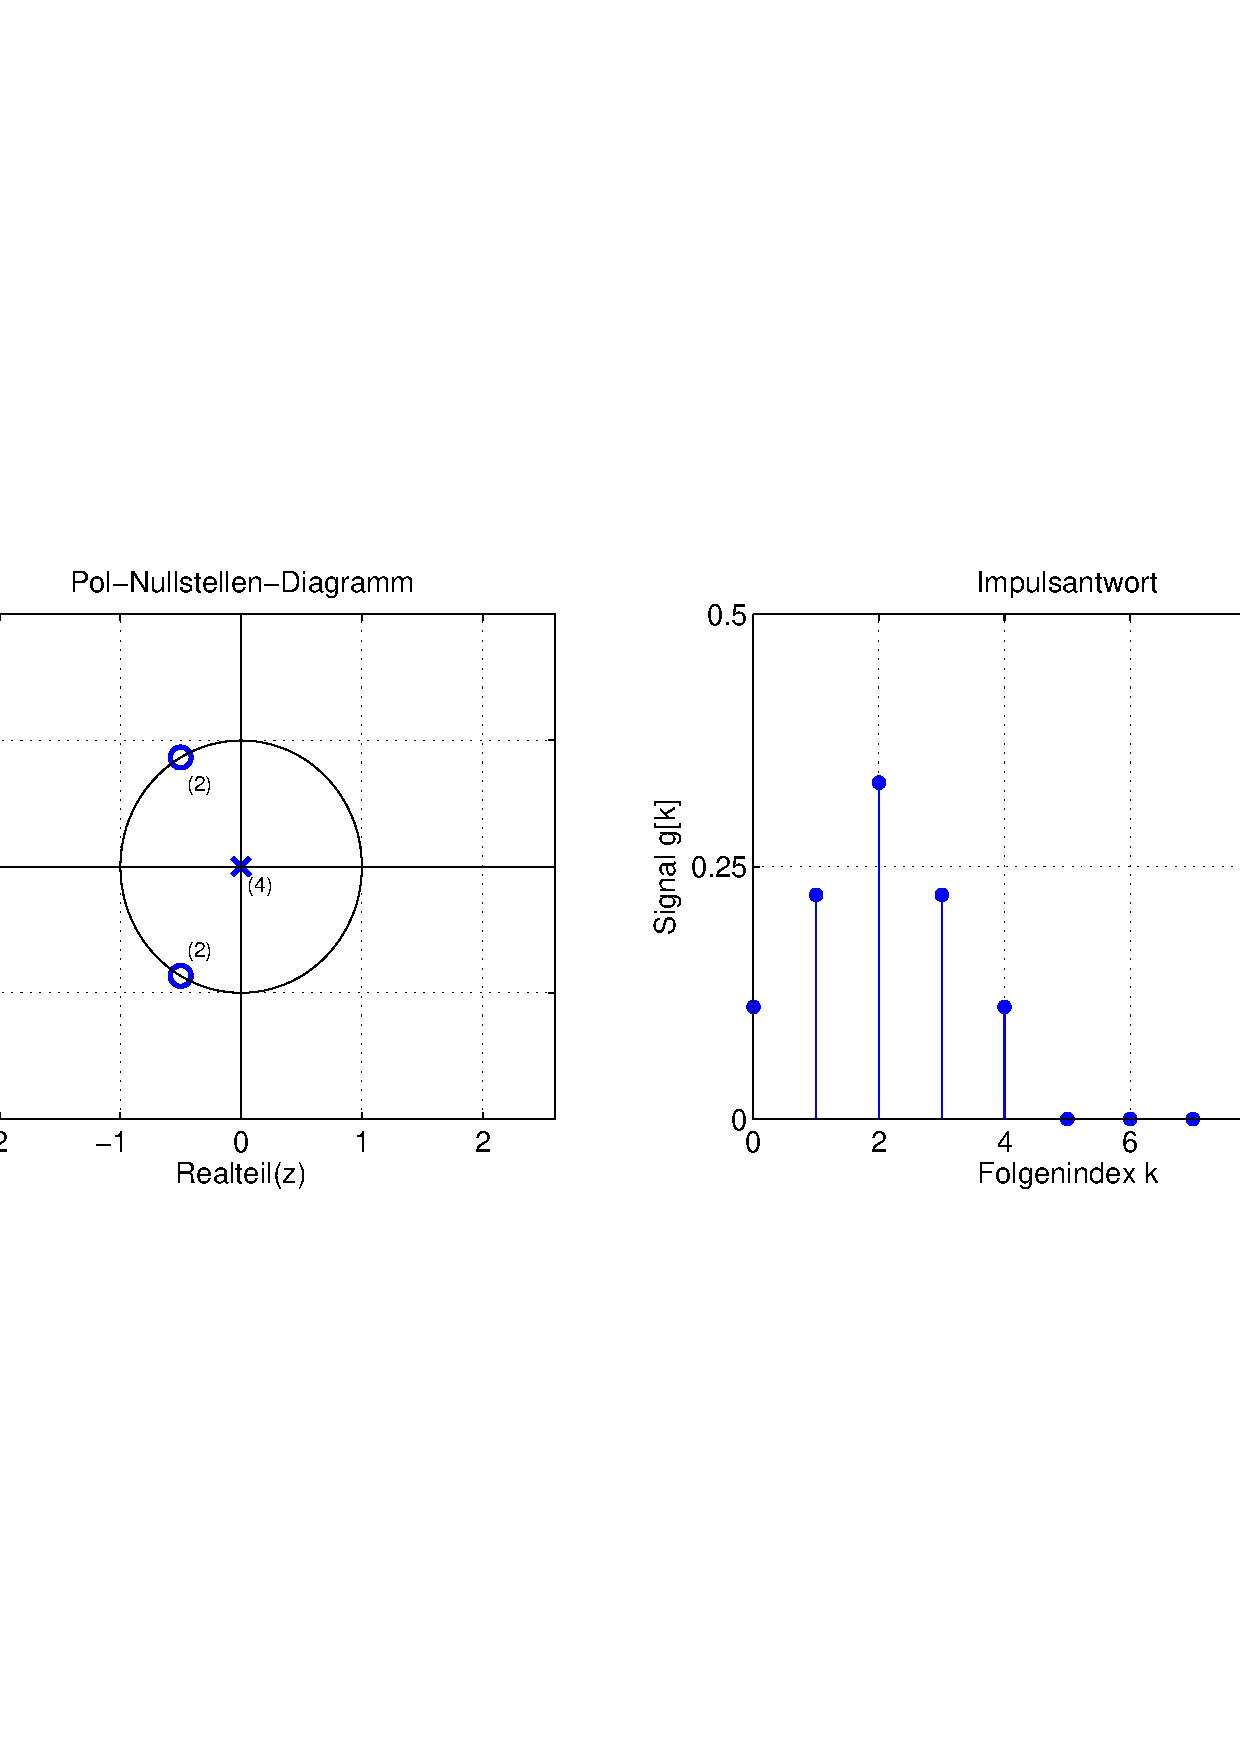
\includegraphics[width=0.05\textwidth]{Kapitel2/Table/image13.png}}} &
\parbox[c][0.9in][c]{1.6in}{\centering{\fontfamily{phv}\selectfont{Demultiplexer}}} &
\parbox[c][0.9in][c]{1.5in}{\centerline{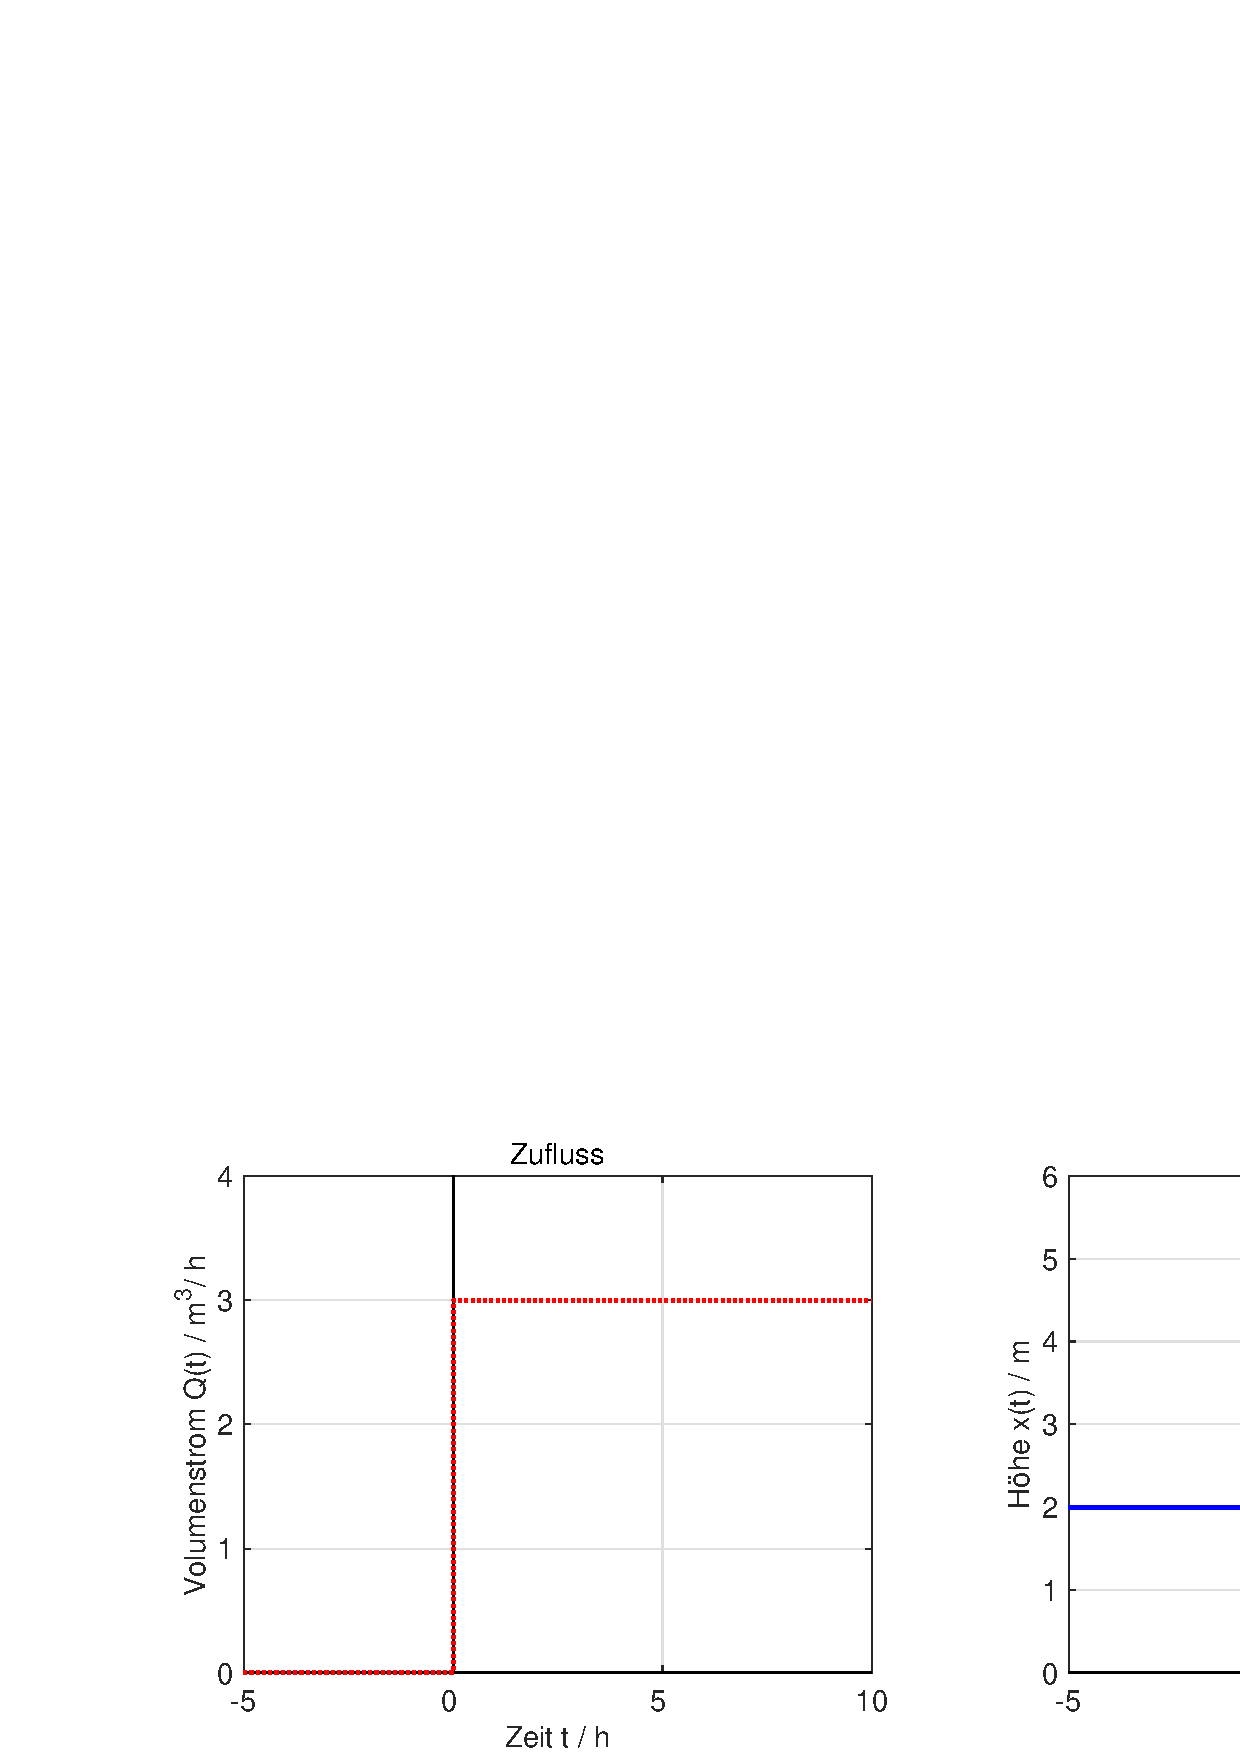
\includegraphics[width=0.05\textwidth]{Kapitel2/Table/image14.png}}} \\ \hline 

\end{tabular}%
}\bigskip
\label{tab:threetwelve}
\end{table}

{\fontfamily{phv}\selectfont
\noindent\textbf{Elementare Übertragungsglieder}}

\noindent Tabelle \ref{tab:threethirteen} zeigt die elementaren Übertragungsglieder zur Darstellung eines linearen, zeitinvarianten Systems als Blockschaltbild.

\begin{table}[H]
\caption{Elementare Übertragungsglieder in Simulink}
\setlength{\fboxsep}{0pt}%
\colorbox{lightgray}{%
\arrayrulecolor{white}%
\begin{tabular}{| c | c | c | c |}
\hline
\parbox[c][0.28in][c]{1.6in}{\smallskip\centering\textbf{\fontfamily{phv}\selectfont{Übertragungsfunktion}}} & \parbox[c][0.28in][c]{1.5in}{\smallskip\centering\textbf{\fontfamily{phv}\selectfont{Simulink Symbol}}} &
\parbox[c][0.28in][c]{1.6in}{\smallskip\centering\textbf{\fontfamily{phv}\selectfont{Übertragungsfunktion}}} &
\parbox[c][0.28in][c]{1.5in}{\smallskip\centering\textbf{\fontfamily{phv}\selectfont{Simulink Symbol}}}\\ \hline

\parbox[c][0.9in][c]{1.6in}{\centering{\fontfamily{phv}\selectfont{Integration}}} &
\parbox[c][0.9in][c]{1.5in}{\centerline{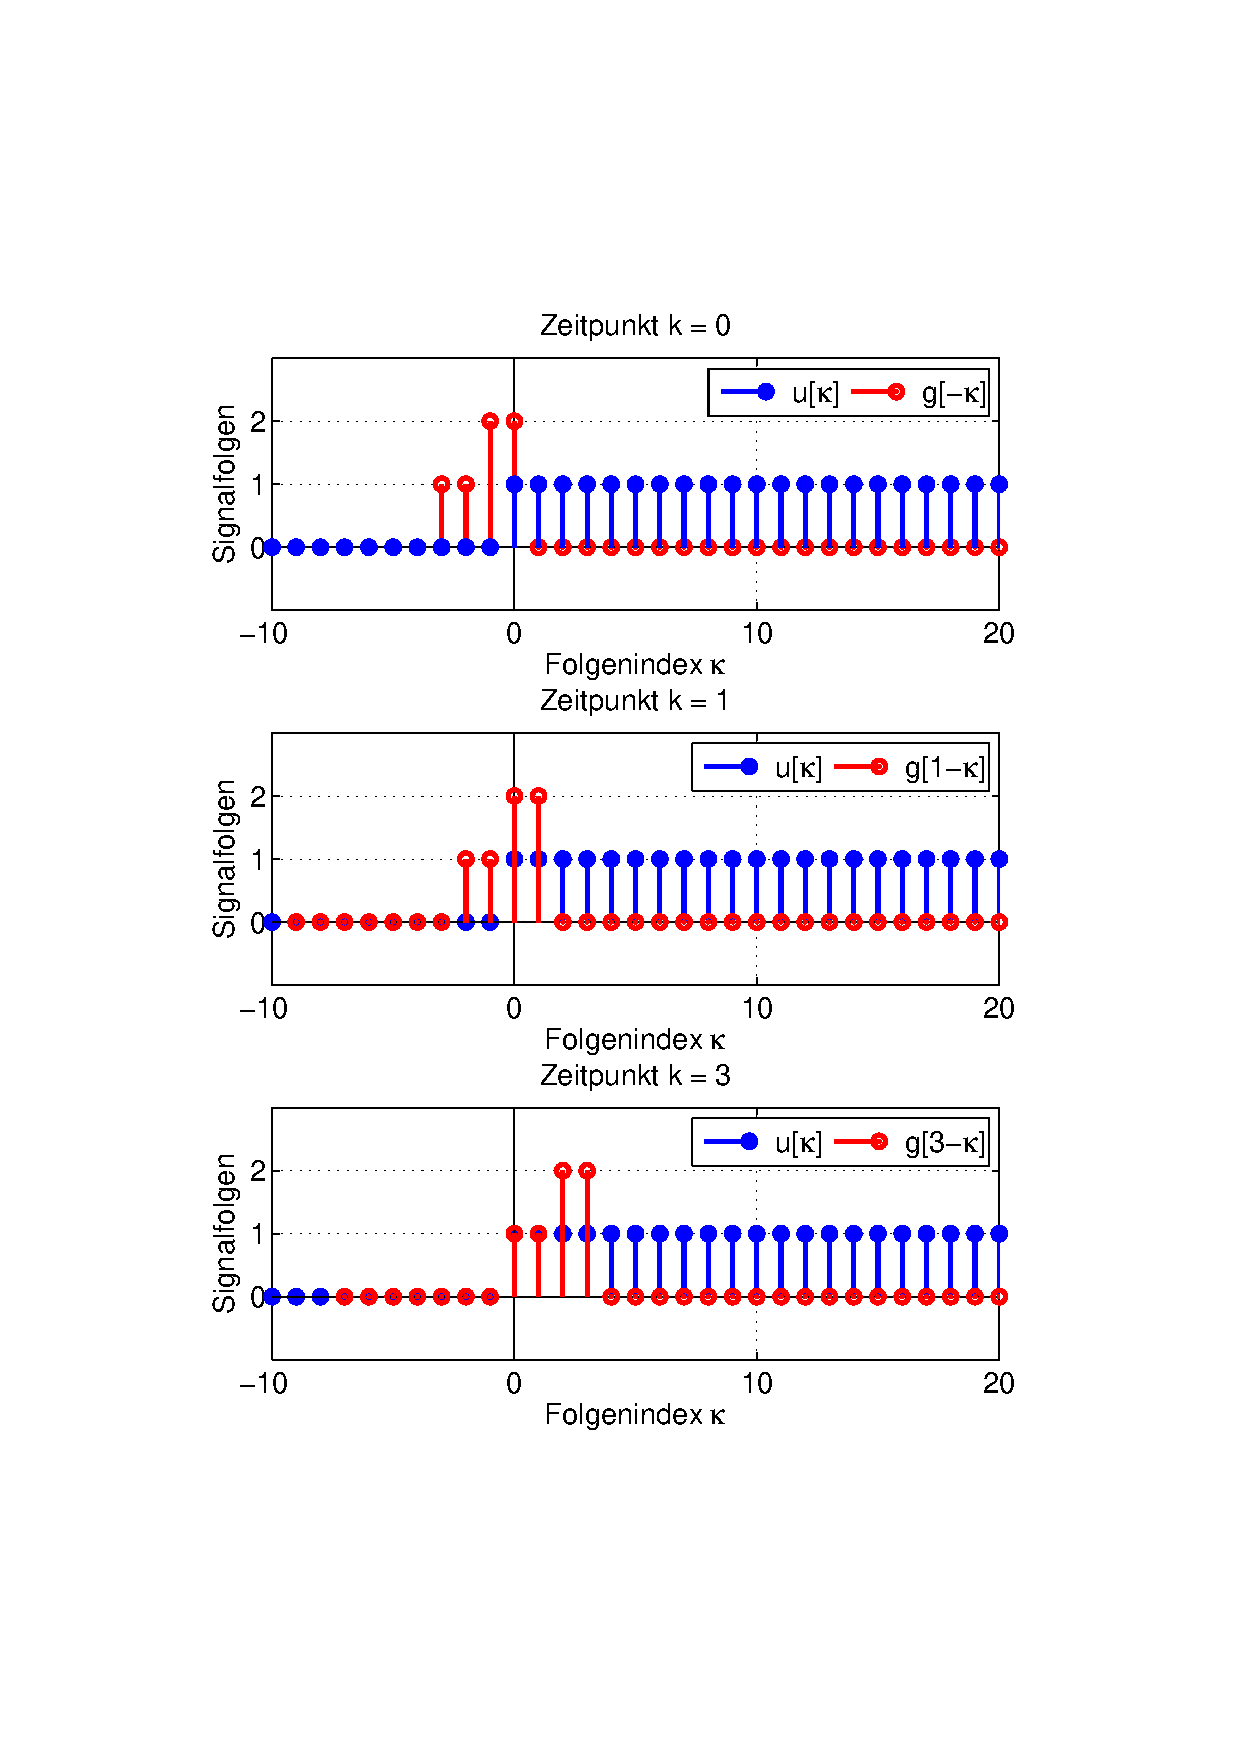
\includegraphics[width=0.1\textwidth]{Kapitel2/Table/image15.png}}} &
\parbox[c][0.9in][c]{1.6in}{\centering{\fontfamily{phv}\selectfont{Differentiation}}} &
\parbox[c][0.9in][c]{1.5in}{\centerline{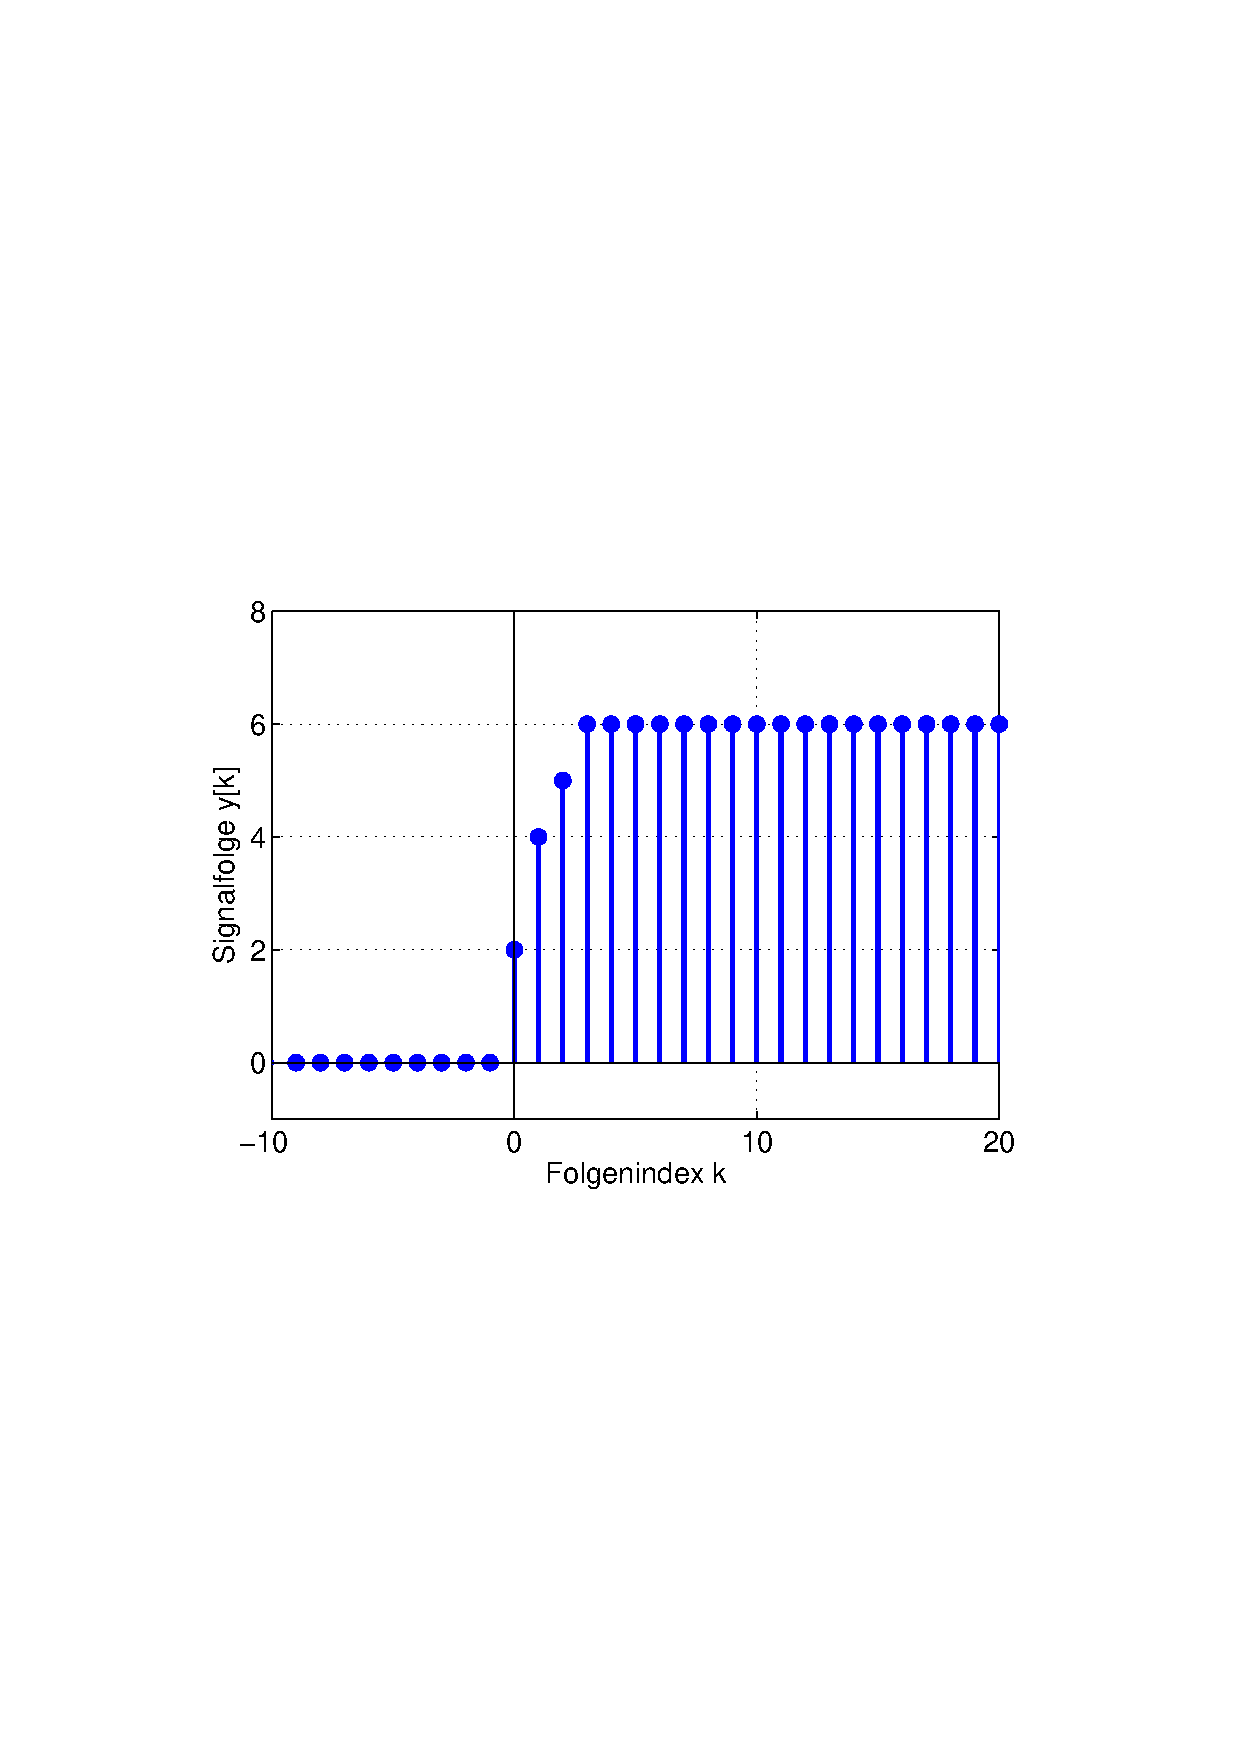
\includegraphics[width=0.1\textwidth]{Kapitel2/Table/image16.png}}} \\ \hline

\end{tabular}%
}\bigskip
\label{tab:threethirteen}
\end{table}

\noindent Integrierer besitzen das Symbol 1/s, im Laplace-Bereich ist das die Übertragungsfunktion eines Integrierers. Durch ein doppeltes Klicken auf die Symbole öffnet sich in Simulink ein Dialog, mit dem die Eigenschaften des Übertragungsglieds definiert werden können. Insbesondere kann bei Integrierern die Anfangsbedingung (\textit{Initial Condition}) festgelegt werden. Wird kein spezieller Anfangswert definiert, verwendet Simulink den Anfangswert y(0) = 0.
\clearpage
\begin{figure}[H]
  \centerline{\includegraphics[width=0.5\textwidth]{Kapitel2/Bilder/image34}}
  \caption{Dialog zur Definition der Eigenschaften eines Integrierers, insbesondere der Anfangsbedingung}
  \label{fig:DialogAnfangsbedingung}
\end{figure}

\noindent Differenzierer sind an dem Symbol du/dt zu erkennen, was auf die zeitliche Ableitung der Eingangsgröße hinweist. Zu Beginn des Abschnitts wird darauf hingewiesen, dass die numerische Realisierung kritisch ist, die Differentiation nicht kausal ist und zu einer Verstärkung von Rauschanteilen im Signal führt. Deshalb sollte auf den Einsatz von Differenzierern verzichtet werden.
Neben den elementaren Übertragungsgliedern Integrierer oder Differenzierer bietet Simulink die Möglichkeit, komplexere Übertragungsglieder im Laplace-Bereich zu definieren. Diese Darstellungsform wird nach der Beschreibung von Systemen im Laplace-Bereich aufgegriffen.

\medskip

{\fontfamily{phv}\selectfont
\noindent\textbf{Signalsenken}}

\noindent Die in Simulink berechneten Signalpfade enden in sogenannten Signalsenken (\textit{Sinks}). Signalsenken stellen das Signal grafisch dar oder speichern das Signal in Variablen oder mat-Files. Tabelle \ref{tab:threefourteen} stellt eine Auswahl von Signalsenken in Simulink dar.

\clearpage

\begin{table}[H]
\caption{Auswahl von Signalsenken in Simulink}
\setlength{\fboxsep}{0pt}%
\colorbox{lightgray}{%
\arrayrulecolor{white}%
\begin{tabular}{| c | c | c | c |}
\hline
\parbox[c][0.28in][c]{1.6in}{\smallskip\centering\textbf{\fontfamily{phv}\selectfont{Signalsenke}}} & \parbox[c][0.28in][c]{1.5in}{\smallskip\centering\textbf{\fontfamily{phv}\selectfont{Simulink Symbol}}} &
\parbox[c][0.28in][c]{1.6in}{\smallskip\centering\textbf{\fontfamily{phv}\selectfont{Signalsenke}}} &
\parbox[c][0.28in][c]{1.5in}{\smallskip\centering\textbf{\fontfamily{phv}\selectfont{Simulink Symbol}}}\\ \hline


\parbox[c][0.9in][c]{1.6in}{\centering{\fontfamily{phv}\selectfont{Numerische Anzeige}}} &
\parbox[c][0.9in][c]{1.5in}{\centerline{\includegraphics[width=0.14\textwidth]{Kapitel2/Table/image17.png}}}  &
\parbox[c][0.9in][c]{1.6in}{\centering{\fontfamily{phv}\selectfont{Grafische Darstellung}}} &
\parbox[c][0.9in][c]{1.5in}{\centerline{\includegraphics[width=0.08\textwidth]{Kapitel2/Table/image18.png}}}\\ \hline

\parbox[c][0.9in][c]{1.2in}{\centering{\fontfamily{phv}\selectfont{Speicherung in Variable im Workspace}}} &
\parbox[c][0.9in][c]{1.5in}{\centerline{\includegraphics[width=0.12\textwidth]{Kapitel2/Table/image19.png}}} &
\parbox[c][0.9in][c]{1.2in}{\centering{\fontfamily{phv}\selectfont{Speicherung in mat-File}}} &
\parbox[c][0.9in][c]{1.5in}{\centerline{\includegraphics[width=0.12\textwidth]{Kapitel2/Table/image20.png}}} \\ \hline

\end{tabular}%
}\bigskip
\label{tab:threefourteen}
\end{table}
\medskip

{\fontfamily{phv}\selectfont
\noindent\textbf{Simulationsvarianten zeitkontinuierlicher Systeme}}\smallskip

\noindent Zeitkontinuierliche Systeme werden in Simulink typischerweise als Variable-Step-Simulation ausgeführt. Dabei bestimmt Simulink auf Basis der Simulationsergebnisse eine variable Schrittweite, die bei vorgegebener Toleranz zu einer minimalen Rechenzeit führt. Die Simulation wird in einem Fenster vorgenommen, das über den Menüpunkt \textit{Simulation / Configuration}  Parameters aufgerufen wird. Es erscheint das Fenster, das in Bild \ref{fig:SimulinkParameters} dargestellt ist.

\begin{figure}[H]
  \centerline{\includegraphics[width=1\textwidth]{Kapitel2/Bilder/image35}}
  \caption{Fenster zur Konfiguration von Parametern in Simulink}
  \label{fig:SimulinkParameters}
\end{figure}

\noindent Für die Simulation sind neben Start- und Endzeitpunkt die Solver-Optionen von Bedeutung. Informationen zu den Eigenschaften der Solver und ihren Anwendungsgebieten sind in [Schw07] und [Stei07] zu finden. Im Rahmen der Vorlesung werden die Simulationen mit dem Solver \textit{ode45 (Dormand-Prince)} ausgeführt. Alle Default-Einstellungen von Simulink werden übernommen.\bigskip

\noindent
\colorbox{lightgray}{%
\arrayrulecolor{white}%
\renewcommand\arraystretch{0.6}%
\begin{tabular}{ wl{16.5cm} }
{\fontfamily{phv}\selectfont
\noindent
Beispiel: Simulation eines Feder-Masse-Dämpfer-Systems}
\end{tabular}%
}\bigskip

\noindent Zur Simulation eines Feder-Masse-Dämpfer-Systems wird das hergeleitete Blockschaltbild mithilfe der
mathematischen Funktionen sowie der Integrierer in MATLAB dargestellt. Es ergibt sich das in Bild \ref{fig:FMDinSimulink} dargestellte Simulink-Modell.

\begin{figure}[H]
  \centerline{\includegraphics[width=0.6\textwidth]{Kapitel2/Bilder/image36}}
  \caption{Blockschaltbild eines Feder-Masse-Dämpfer-Systems in Simulink }
  \label{fig:FMDinSimulink}
\end{figure}

\noindent Als Signalquelle wird eine Sprungfunktion eingesetzt. Ein- und Ausgangssignal werden in einem sogenannten \textit{Scope}  dargestellt. Für eine Federkonstante von c = 100 N/m, eine Dämpfung von D = 0.5 N$\cdot$s/m, eine Masse m = 10 g und eine Kraft F0 = 0.2 N ergibt sich das in Bild \ref{fig:SimulationFDM} \textit{Scope}-Bild.

\begin{figure}[H]
  \centerline{\includegraphics[width=0.5\textwidth]{Kapitel2/Bilder/image37}}
  \caption{Simulation des Einschwingverhaltens des Feder-Masse-Dämpfer-Systems bei einer sprungförmigen Anre-gung mit einer Kraft von 0.2 N dargestellt als Scope in Simulink}
  \label{fig:SimulationFDM}
\end{figure}

\noindent Das Eingangssignal ist in dem oberen Feld als Sprung zu erkennen. Das Ausgangssignal ist im unteren Feld dargestellt. Das Simulationsergebnis entspricht dem in Bild \ref{fig:SimulationFDM} dargestellten Signalverlauf.

\clearpage

\subsection{Literatur}


\subsubsection{Literaturstellen mit anschaulicher Darstellung}

\begin{tabular}{|p{0.6in}|p{5.7in}|} \hline 
[Alba04] & Albach, Manfred: Grundlagen der Elektrotechnik 1und 2.\\ 
& Pearson Studium, 2004 \\ \hline 
[Foel11] & Föllinger, Otto: Laplace-, Fourier- und z-Transformation. 10., überarbeitete Auflage \\ 
& VDE Verlag GmbH, Berlin, Offenbach 2011 \\ \hline 
[Führ06] & Führer, Arnold: Grundgebiete der Elektrotechnik 1 - 3 \\
& Hanser Verlag, München, 2006\\ \hline 
[Goeb11] & Goebbels, Steffen: Mathematik verstehen und anwenden \\
& Spektrum Akademischer Verlag, Heidelberg, 2011 \\ \hline 
[Papu01] & Papula, Lothar: Mathematik für Ingenieure und Naturwissenschaftler \\
& Vieweg Fachbücher der Technik, Braunschweig/Wiesbaden, 2001 \\ \hline 
\end{tabular}


\subsubsection{Literatur zu MATLAB}

\begin{tabular}{|p{0.6in}|p{5.7in}|} \hline 
[Beuc00] & Beucher, Ottmar: MATLAB und Simulink lernen,\\
& Addison Wesley Longman Verlag, München, 2000\\ \hline 
[Schw07] & Schweizer, Wolfgang: MATLAB kompakt, \\ 
& Oldenbourg Verlag München, 2007\\ \hline 
[Stei07] & Stein, Ulrich: Einstieg in das Programmieren mit MATLAB,\\
& Fachbuchverlag Leipzig, 2007\\ \hline 
\end{tabular}


\subsubsection{Literaturstellen mit praktischen Anwendungen mit MATLAB}

\begin{tabular}{|p{0.6in}|p{5.7in}|} \hline 
[Hoff98] & Hoffmann, Josef: Matlab und Simulink, \\
& Addison Wesley Longman Verlag, München, 1998\\ \hline 
[Hoff99] & Hoffmann, Josef: Matlab und Simulink in der Signalverarbeitung und \\
& Kommunikationstechnik, Addison Wesley Longman Verlag, München, 1999\\ \hline 
[Sche04] & Scherf, Helmut: Modellbildung und Simulation dynamischer Systeme,\\
& Oldenbourg Verlag, München, 2004\\ \hline 
\end{tabular}


\subsubsection{Weiterführende Literatur}

\begin{tabular}{|p{0.6in}|p{5.7in}|} \hline 
[Bart89] & Barton, G.: Elements of Green's Functions and Propagation: Potentials, Diffusion, and\\
&   Waves, Oxford University Press, 1989\\ \hline 
\end{tabular}